\documentclass[12pt,a4paper]{report}

\usepackage[utf8]{inputenc}
\usepackage[T1]{fontenc}
\usepackage{underscore}
\usepackage{listings}
\lstdefinelanguage{Solidity}{
  keywords={pragma,solidity,contract,function,returns,external,internal,public,private,
             view,pure,payable,mapping,address,uint256,uint,bool,bytes32,string,
             event,emit,modifier,require,revert,import,is,memory,storage,indexed,
             bytes,keccak256,struct,enum,constructor,fallback,receive},
  sensitive=true,
  comment=[l]{//},
  morecomment=[s]{/*}{*/},
  morestring=[b]",
}
\lstset{
  basicstyle=\ttfamily\scriptsize,
  keywordstyle=\bfseries,
  commentstyle=\color{black!55}\itshape,
  stringstyle=\itshape,
  breaklines=true,
  frame=tb,
  rulecolor=\color{black!55},
  captionpos=b,
  numbers=left,
  numberstyle=\tiny\color{black!55},
  xleftmargin=2em,
}
\IfFileExists{libertine.sty}{%
  \usepackage[mono=false]{libertine}%
  \IfFileExists{zi4.sty}{\usepackage[varqu]{zi4}}{}%
}{%
  \usepackage{lmodern}%
}
\usepackage[protrusion=true,expansion=false]{microtype}
\usepackage[a4paper,width=155mm,top=25mm,bottom=25mm,headheight=15pt]{geometry}
\usepackage{setspace}
\onehalfspacing
\emergencystretch=3em
\hbadness=2000

\usepackage{amsmath,amssymb}
\usepackage{fontawesome5}
\newcommand{\tmarkDone}{\textbf{\faCheck}}
\newcommand{\tmarkNo}{\textbf{\faTimes}}
\newcommand{\tmarkPartial}{\faHourglassHalf}
\newcommand{\tmarkPlanned}{\textcolor{black!55}{\faCircle}}

\usepackage{graphicx}
\usepackage{pdflscape} % full-page landscape for wide ER diagrams
% Self-contained build: figure assets in Diagrams/ (SVG sources; LaTeX includes generated PDF).
% Rebuild PDFs:  ./Diagrams/build-pdfs.sh
% Compile from this directory:  pdflatex Pre-thesis_v33.tex (twice)
\newcommand*{\ThesisDiagDir}{Diagrams/}
\newcommand*{\ThesisNewDiagDir}{mermaid-diagrams/pdf/}
\graphicspath{{\ThesisNewDiagDir}{./\ThesisNewDiagDir}{\ThesisDiagDir}{./\ThesisDiagDir}{./}{Tables/}}
\pdfimageresolution=300
\makeatletter
\newcommand*{\@thesis@doinclude}[2]{%
  \if\relax\detokenize{#1}\relax
    \includegraphics{#2}%
  \else
    \includegraphics[#1]{#2}%
  \fi
}
\newcommand*{\@thesismissingimg}[1]{%
  \fbox{\parbox{0.92\linewidth}{\scriptsize\centering\ttfamily Missing diagram: \detokenize{\ThesisDiagDir#1}.\\[2pt]Add \texttt{#1} (from matching \texttt{.svg} via \texttt{build-pdfs.sh}) to \texttt{Diagrams/} and recompile.}}%
}
\newcommand*{\@thesis@loadfig}[2]{%
  \IfFileExists{\ThesisDiagDir#2}{%
    \@thesis@doinclude{#1}{\ThesisDiagDir#2}}{%
  \IfFileExists{#2}{%
    \@thesis@doinclude{#1}{#2}}{%
  \IfFileExists{Tables/#2}{%
    \@thesis@doinclude{#1}{Tables/#2}}{%
    \@thesismissingimg{#2}%
  }}}%
}
\newcommand{\ThesisIncludeGraphics}[2][]{%
  \IfFileExists{\ThesisNewDiagDir#2.pdf}{%
    \@thesis@doinclude{#1}{\ThesisNewDiagDir#2.pdf}}{%
  \IfFileExists{\ThesisDiagDir#2.pdf}{%
    \@thesis@doinclude{#1}{\ThesisDiagDir#2.pdf}}{%
  \@thesis@loadfig{#1}{#2}%
  }}%
}
% Shorthand: \Diagram{stem} -> Diagrams/stem.pdf
\newcommand{\Diagram}[2][]{%
  \if\relax\detokenize{#1}\relax
    \ThesisIncludeGraphics{#2}%
  \else
    \ThesisIncludeGraphics[#1]{#2}%
  \fi
}
\makeatother
\newcommand{\TableScreenshotEnd}[2][]{%
  \refstepcounter{table}%
  \if\relax\detokenize{#1}\relax\else\label{#1}\fi%
  \phantomsection%
  \addcontentsline{lot}{table}{\protect\numberline{\thetable}#2}%
}
\usepackage[table]{xcolor}
\usepackage{tikz}
\usetikzlibrary{arrows.meta,positioning,fit,shapes.geometric,calc}
\usepackage{pgfplots}
\usepgfplotslibrary{statistics}
\pgfplotsset{compat=1.18, minor tick num=0}

\usepackage{booktabs}
\usepackage{array}
\usepackage{colortbl}
\usepackage{multirow}
\usepackage{float}
\usepackage{etoolbox}
\usepackage{caption}
\captionsetup{
    labelfont={bf,small},
    textfont={small},
    skip=6pt,
    format=hang
}
\makeatletter
% Compact, professional List of Figures / List of Tables (no tocloft dependency)
\renewcommand*\l@figure{\@dottedtocline{1}{0em}{3.2em}}
\renewcommand*\l@table{\@dottedtocline{1}{0em}{3.8em}}
\makeatother

\newlength{\ThesisTableImgReserve}
\newlength{\ThesisFigImgReserve}
\setlength{\ThesisTableImgReserve}{\dimexpr2\intextsep+0.75\baselineskip\relax}
\setlength{\ThesisFigImgReserve}{\dimexpr2\intextsep+\abovecaptionskip+\belowcaptionskip+4\baselineskip\relax}
\newcommand{\TableImageMaxFit}[1]{%
  \ThesisIncludeGraphics[
    width=0.7\linewidth,
    height=\dimexpr(\textheight-\ThesisTableImgReserve)*7/10\relax,
    keepaspectratio
  ]{#1}%
}
\newcommand{\FigureImageMaxFit}[1]{%
  \ThesisIncludeGraphics[width=\linewidth,height=\dimexpr\textheight-\ThesisFigImgReserve\relax,keepaspectratio]{#1}%
}
\newcommand{\OnePageDiagram}[2][]{%
  \if\relax\detokenize{#1}\relax
    \ThesisIncludeGraphics[width=\linewidth,height=\dimexpr\textheight-\ThesisFigImgReserve\relax,keepaspectratio]{#2}%
  \else
    \ThesisIncludeGraphics[#1,width=\linewidth,height=\dimexpr\textheight-\ThesisFigImgReserve\relax,keepaspectratio]{#2}%
  \fi
}
\newcommand{\HalfWidthDiagram}[1]{%
  \ThesisIncludeGraphics[width=0.5\linewidth,keepaspectratio]{#1}%
}
\newcommand{\WideDiagram}[2][]{%
  \if\relax\detokenize{#1}\relax
    \ThesisIncludeGraphics[width=\linewidth,height=0.78\textheight,keepaspectratio]{#2}%
  \else
    \ThesisIncludeGraphics[#1,width=\linewidth,height=0.78\textheight,keepaspectratio]{#2}%
  \fi
}
\newcommand{\TallDiagram}[2][]{%
  \if\relax\detokenize{#1}\relax
    \ThesisIncludeGraphics[width=\linewidth,height=0.96\textheight,keepaspectratio]{#2}%
  \else
    \ThesisIncludeGraphics[#1,width=\linewidth,height=0.96\textheight,keepaspectratio]{#2}%
  \fi
}
% Balanced layout slot (reference: Figure 4.3 ml-explainability) — wide banded diagrams.
\newcommand{\BalancedDiagram}[2][]{%
  \if\relax\detokenize{#1}\relax
    \ThesisIncludeGraphics[width=\linewidth,height=0.72\textheight,keepaspectratio]{#2}%
  \else
    \ThesisIncludeGraphics[#1,height=0.72\textheight,keepaspectratio]{#2}%
  \fi
}
% Activity diagrams — full-height slot for 3× label size.
\newcommand{\ActivityDiagram}[2][]{%
  \if\relax\detokenize{#1}\relax
    \ThesisIncludeGraphics[width=\linewidth,height=0.88\textheight,keepaspectratio]{#2}%
  \else
    \ThesisIncludeGraphics[#1,height=0.88\textheight,keepaspectratio]{#2}%
  \fi
}
% Half-size slot (50\% of BalancedDiagram width and height).
\newcommand{\CompactDiagram}[2][]{%
  \if\relax\detokenize{#1}\relax
    \ThesisIncludeGraphics[width=0.5\linewidth,height=0.36\textheight,keepaspectratio]{#2}%
  \else
    \ThesisIncludeGraphics[#1,width=0.5\linewidth,height=0.36\textheight,keepaspectratio]{#2}%
  \fi
}

\usepackage[skins]{tcolorbox}

\usepackage{titlesec}
\usepackage{parskip}
\usepackage{fancyhdr}
\usepackage{enumitem}
\PassOptionsToPackage{hyphens,spaces,obeyspaces}{url}
\usepackage{hyperref}
\makeatletter
\g@addto@macro\UrlBreaks{\do\/\do\-\do\.\do\:\do\&\do\=\do\#}
\makeatother

\definecolor{PrimaryBlue}{HTML}{000000}
\definecolor{AccentBlue}{gray}{0.55}
\definecolor{LightBlue}{gray}{0.96}
\definecolor{MidBlue}{gray}{0.90}
\definecolor{DarkText}{HTML}{000000}
\definecolor{GrayText}{gray}{0.45}
\definecolor{RowShade}{gray}{0.965}
\definecolor{RowShadeAlt}{gray}{0.92}
\definecolor{TableHeadBg}{gray}{0.88}
\definecolor{TableRule}{gray}{0.55}
\definecolor{GreenAccent}{HTML}{000000}
\definecolor{AmberAccent}{HTML}{000000}
\definecolor{RedAccent}{HTML}{000000}
\definecolor{VioletAccent}{HTML}{000000}

\hypersetup{
    colorlinks=true,
    linkcolor=black,
    filecolor=black,
    urlcolor=black,
    citecolor=black,
    pdfborder={0 0 0},
}

\titleformat{\chapter}[display]
    {\normalfont\LARGE\bfseries}
    {\chaptertitlename\ \thechapter}{20pt}{\LARGE}
    [\vspace{4pt}{\color{black!40}\titlerule[0.6pt]}]

\titleformat{\section}
    {\large\bfseries}
    {\thesection}{0.8em}{}

\titleformat{\subsection}
    {\normalsize\bfseries}
    {\thesubsection}{0.6em}{}

\titleformat{\subsubsection}
    {\normalsize\bfseries\itshape}
    {\thesubsubsection}{0.6em}{}

\titlespacing*{\chapter}{0pt}{-20pt}{20pt}
\titlespacing*{\section}{0pt}{16pt plus 3pt minus 2pt}{8pt plus 2pt minus 1pt}
\titlespacing*{\subsection}{0pt}{12pt plus 2pt minus 1pt}{6pt plus 1pt minus 1pt}
\titlespacing*{\subsubsection}{0pt}{10pt plus 2pt minus 1pt}{4pt plus 1pt minus 1pt}

\newcommand{\tableheadcolor}{\rowcolor{TableHeadBg}}
\newcommand{\tableheadfont}{\bfseries}
\newcommand{\ThesisTableBodyFont}{\small}

% Consistent greyscale table polish (font size unchanged; spacing only).
\newcommand{\ThesisTablePrep}{%
  \ThesisTableBodyFont
  \renewcommand{\arraystretch}{1.22}%
  \setlength{\tabcolsep}{6pt}%
  \arrayrulecolor{TableRule}%
  \setlength{\aboverulesep}{0.55ex}%
  \setlength{\belowrulesep}{0.55ex}%
}
\AtBeginEnvironment{table}{\ThesisTablePrep}
\AtBeginEnvironment{tabular}{%
  \rowcolors{2}{}{RowShade}%
  \arrayrulecolor{TableRule}%
}

\newenvironment{moderntable}[1][H]{%
    \begin{table}[#1]\centering\ThesisTablePrep
}{%
    \end{table}%
}

\newtcolorbox{layerbox}[1]{
    colback=white,
    colframe=black!55,
    coltitle=black,
    fonttitle=\bfseries\small,
    title=#1,
    boxrule=0.6pt,
    arc=2pt,
    left=6pt,right=6pt,top=4pt,bottom=4pt,
}

\newtcolorbox{highlightbox}[1][]{
    colback=black!4,
    colframe=black!45,
    boxrule=0.5pt,
    arc=2pt,
    left=8pt,right=8pt,top=6pt,bottom=6pt,
    #1
}

\pagestyle{fancy}
\fancyhf{}
\renewcommand{\headrulewidth}{0.4pt}
\fancyhead[L]{\small\color{black!55}Crypto World Bank}
\fancyhead[R]{\small\color{black!55}BRAC University}
\fancyfoot[C]{\small\color{black!55}\thepage}

\newcommand{\manualpie}[6]{%
  \fill[#6] (#1,#2) -- ++({#4}:{#3}) arc ({#4}:{#5}:{#3}) -- cycle;
  \draw[white, line width=0.8pt] (#1,#2) -- ++({#4}:{#3}) arc ({#4}:{#5}:{#3}) -- cycle;
}
\newcommand{\ddcat}[3]{\node[draw=black!55,fill=black!5,rounded corners=2pt,
  minimum width=2.2cm,minimum height=0.65cm,align=center,font=\scriptsize]
  (#1) at (#2) {#3};}
\newcommand{\ddone}[3]{\node[draw=black,fill=black!22,
  minimum width=2.2cm,minimum height=0.65cm,align=center,
  font=\scriptsize\bfseries,rounded corners=2pt] (#1) at #2 {#3};}
\newcommand{\ddtwo}[3]{\node[draw=black!55,fill=white,
  minimum width=2.2cm,minimum height=0.65cm,align=center,
  font=\scriptsize,rounded corners=2pt] (#1) at #2 {#3};}

\begin{document}

%% ============================================================
%% TITLE PAGE
%% ============================================================
\thispagestyle{empty}

\begin{center}

\vspace*{0.3cm}

\ThesisIncludeGraphics[width=3.5cm]{bracu\_logo\_12-0-2022}

\vspace{0.8cm}

{\LARGE\bfseries\color{PrimaryBlue} Decentralized Crypto World Bank}\\[0.4em]
{\large\color{PrimaryBlue!80} A Blockchain-Based Banking Platform\\[0.15em]with AI-Enhanced Security and Assistance}

\vspace{1.2cm}

{\large by}

\vspace{0.5cm}

{\Large\bfseries\color{PrimaryBlue} Md.\ Bokhtiar Rahman Juboraz}\\[0.2em]
{\color{GrayText}20301138}\\[0.8em]
{\Large\bfseries\color{PrimaryBlue} Md.\ Mahir Ahnaf Ahmed}\\[0.2em]
{\color{GrayText}20301083}

\vspace{1.2cm}

A pre-thesis 1 report submitted to the Department of Computer Science and Engineering\\
in partial fulfillment of the requirements for the degree of\\
\textbf{B.Sc.\ in Computer Science}

\vfill

{\color{PrimaryBlue}\rule{0.4\textwidth}{0.6pt}}\\[0.6em]
Department of Computer Science and Engineering\\
\textbf{BRAC University}\\
February 2026

\vspace{0.5cm}

{\small\color{GrayText}\copyright\ 2026.\ BRAC University --- All rights reserved.}

\end{center}

%% ============================================================
%% DECLARATION
%% ============================================================
\newpage
\thispagestyle{empty}

\chapter*{Declaration}
\phantomsection
\addcontentsline{toc}{chapter}{Declaration}

It is hereby declared that

\begin{enumerate}
\item The report submitted is our own original work while completing degree at BRAC University.

\item The report does not contain material previously published or written by a third party, except where this is appropriately cited through full and accurate referencing.

\item The report does not contain material which has been accepted, or submitted, for any other degree or diploma at a university or other institution.

\item We have acknowledged all main sources of help.
\end{enumerate}

\vspace{2cm}

\textbf{Student's Full Name \& Signature:}

\vspace{2cm}

\begin{tabular}{p{6cm}p{1cm}p{6cm}}
\hrulefill & & \hrulefill \\
\centering Md. Bokhtiar Rahman Juboraz & & \centering Md. Mahir Ahnaf Ahmed \tabularnewline
\centering 20301138 & & \centering 20301083 \tabularnewline
\end{tabular}

%% ============================================================
%% APPROVAL
%% ============================================================
\newpage
\thispagestyle{empty}

\chapter*{Approval}
\phantomsection
\addcontentsline{toc}{chapter}{Approval}

The pre-thesis 1 report of final year project titled ``Decentralized Crypto World Bank: A Blockchain-Based Banking Platform with AI-Enhanced Security and Assistance'' submitted by

\begin{enumerate}
\item Md. Bokhtiar Rahman Juboraz (20301138)
\item Md. Mahir Ahnaf Ahmed (20301083)
\end{enumerate}

Of Spring, 2026 has been accepted as satisfactory in partial fulfillment of the requirement for the degree of B.Sc. in Computer Science on February 20, 2026.

\vspace{1cm}

\textbf{Examining Committee:}

\vspace{1.5cm}

\begin{flushleft}
Supervisor:\\
(Member)
\end{flushleft}

\begin{flushright}
\vspace{-0.5cm}
\hrulefill\\
Mr. Annajiat Alim Rasel\\
Senior Lecturer\\
Department of Computer Science and Engineering\\
BRAC University
\end{flushright}

\vspace{1.5cm}

\begin{flushleft}
Project Coordinator:\\
(Member)
\end{flushleft}

\begin{flushright}
\vspace{-0.5cm}
\hrulefill\\
Dr. Md. Golam Rabiul Alam\\
Professor\\
Department of Computer Science and Engineering\\
BRAC University
\end{flushright}

\newpage

\vspace{1.5cm}

\begin{flushleft}
Head of Department:\\
(Chair)
\end{flushleft}

\begin{flushright}
\vspace{-0.5cm}
\hrulefill\\
Dr. Sadia Hamid Kazi\\
Chairperson and Associate Professor\\
Department of Computer Science and Engineering\\
BRAC University
\end{flushright}

%% ============================================================
%% ETHICS STATEMENT
%% ============================================================
\newpage
\thispagestyle{empty}

\chapter*{Ethics Statement}
\phantomsection
\addcontentsline{toc}{chapter}{Ethics Statement}

This project operates exclusively on public blockchain test networks using test tokens with no real monetary value. No real financial transactions, personal banking data, or user financial records are involved at any stage of development or evaluation. All transaction data used for Artificial Intelligence and Machine Learning (AI/ML) model training and evaluation is either synthetically generated or sourced from publicly available anonymized datasets. The platform prototype does not process Know Your Customer (KYC) or Anti-Money Laundering (AML) data in its current scope, and all wallet addresses used during testing are disposable testnet addresses. We acknowledge the ethical considerations inherent in AI-assisted financial decision-making and have incorporated explainability mechanisms (SHapley Additive exPlanations, or SHAP) to ensure that automated risk assessments remain transparent and auditable by human reviewers. Future phases plan to incorporate a privacy-preserving ZKP-based identity compliance layer in which users prove KYC status without exposing personal data on-chain; the ethical implications of this design will be evaluated in the final thesis.

%% ============================================================
%% ABSTRACT
%% ============================================================
\newpage
\thispagestyle{empty}

\chapter*{Abstract}
\phantomsection
\addcontentsline{toc}{chapter}{Abstract}

Development finance moves capital through several institutional layers, but settlement is often slow, costly, and hard to audit. Decentralized finance (DeFi) can automate lending on-chain, yet most protocols use flat pools that do not match real tiered banking. \textit{Crypto World Bank} (CWB) is a research prototype that specifies a four-tier lending platform on EVM-compatible infrastructure: World Bank Reserve $\to$ National Bank $\to$ Local Bank $\to$ Client.

The design pairs on-chain reserve rules and role-based access with off-chain KYC and ML risk scoring (Random Forest, Isolation Forest, SHAP), committed through a commit--reveal oracle. A conversational agent (Qwen3-8B + MCP) is planned as an optional plain-language UI. At pre-thesis stage, the main output is formal specification and a four-phase build plan. Measured ML results come from a synthetic BCCC-shaped validation run; full BCCC-DeFiFraudTrans-2025 retraining is planned after York dataset access (request submitted). Final-thesis targets include testnet loan lifecycle, latency and gas tables, reserve invariant tests, and a small agent demo with a human confirmation gate.

\vspace{0.5em}
\noindent\textbf{Keywords:} Blockchain, DeFi, Institutional Finance, Hierarchical Lending, Smart Contracts, Explainable AI, Group Lending

%% ============================================================
%% DEDICATION
%% ============================================================
\newpage
\thispagestyle{empty}

\chapter*{Dedication}
\phantomsection
\addcontentsline{toc}{chapter}{Dedication}

\vspace{3cm}
\begin{center}
\textit{Dedicated to our families for their unwavering support throughout our academic journey.}
\end{center}

%% ============================================================
%% ACKNOWLEDGMENT
%% ============================================================
\newpage
\thispagestyle{empty}

\chapter*{Acknowledgment}
\phantomsection
\addcontentsline{toc}{chapter}{Acknowledgment}

We would like to express our sincere gratitude to our panel members for their guidance and support throughout this project. We also thank our supervisor, Mr.\ Annajiat Alim Rasel, Senior Lecturer at the Department of Computer Science and Engineering, BRAC University, for his guidance and support. Finally, we thank the Department of Computer Science and Engineering at BRAC University for providing us with the resources and academic environment to pursue this work.

%% ============================================================
%% TABLE OF CONTENTS, LIST OF TABLES, LIST OF FIGURES
%% ============================================================
\newpage
\singlespacing
\setcounter{page}{1}
\pagenumbering{roman}
\tableofcontents
\newpage
\phantomsection
\addcontentsline{toc}{chapter}{List of Tables}
\listoftables
\newpage
\phantomsection
\addcontentsline{toc}{chapter}{List of Figures}
\listoffigures
\newpage
\chapter*{List of Formulas}
\phantomsection
\addcontentsline{toc}{chapter}{List of Formulas}
\begin{description}[leftmargin=0pt]
    \item[Utilization ($U$):] \(U = \frac{L}{L + B}\)
    \item[Kinked rate ($U \leq U^*$):] \(r_b(U) = r_0 + \frac{U}{U^*} \cdot r_1\)
    \item[Kinked rate ($U > U^*$):] \(r_b(U) = r_0 + r_1 + \frac{U - U^*}{1 - U^*} \cdot r_2\)
    \item[Collateral Ratio:] \(CR = \frac{C}{D}\)
    \item[Loan-to-Value:] \(LTV = \frac{\text{Loan Amount}}{\text{Collateral Value}}\)
    \item[APR (simple):] \(APR = r_{\text{period}} \times N\)
    \item[Compound interest:] \(A = P\left(1 + \frac{r}{n}\right)^{nt}\)
    \item[EMI:] \(EMI = \frac{P \cdot r \cdot (1+r)^n}{(1+r)^n - 1}\)
    \item[Health Factor:] \(HF = \frac{C \times LT}{D}\)
    \item[Group Health Factor:] \(HF_{\text{group}} = \frac{\text{total\_group\_collateral} \times LT}{\text{total\_group\_outstanding\_debt}}\)
    \item[Institutional Health Factor:] \(HF_{\text{inst}} = \frac{\text{on\_chain\_reserve} - \text{min\_reserve}}{\text{outstanding\_borrowing}}\)
    \item[Reserve Ratio:] \(RR = \frac{\text{Reserves}}{\text{Total Deposits}}\)
    \item[Platform Solvency Ratio:] \(PSR = \frac{\text{TotalReserveBalance}}{\text{TotalOutstandingLoans}}\)
    \item[Credit Velocity:] \(CV = \frac{\text{Capital Recycled per Period}}{\text{Total Reserve}}\)
    \item[Interbank rate cap:] \(r_{\text{IB}}(U) \leq r_{\text{downward}}(U) - \delta\)
    \item[Upward deposit rate cap:] \(r_{\text{up}} < r_{\text{down}} - \delta\)
    \item[FX conversion:] \(\text{Amount}_B = \text{Amount}_A \times \frac{P_A}{P_B}\)
    \item[Treasury swap:] \(\text{Amount}_{\text{to}} = \text{Amount}_{\text{from}} \times \frac{P_{\text{from}}}{P_{\text{to}}} \times (1 - \text{spread})\)
    \item[Oracle commit--reveal:] \(h = \text{keccak256}(s \,\|\, \text{nonce})\)
    \item[Group loan share:] \(\text{Share}_i = \frac{\text{LoanTotal}}{N_{\text{members}}}\)
    \item[On-chain credit score:] \(CS = \sum_i w_i \cdot \text{feature}_i\)
    \item[Isolation Forest score:] \(s(x, n) = 2^{-E(h(x))/c(n)}\)
    \item[Random Forest fraud probability:] \(P(\text{fraud}\mid x) = \frac{1}{T}\sum_{t=1}^{T} f_t(x)\)
    \item[Net interest split:] \(\text{NetInterest} = \text{InterestCollected} - \text{DepositorYield} - \text{InsuranceAllocation}\)
    \item[SHAP (Shapley value):] \(\phi_i = \sum_{S \subseteq F \setminus \{i\}} \frac{|S|!(|F|-|S|-1)!}{|F|!}\left[f(S \cup \{i\}) - f(S)\right]\)
\end{description}
\newpage
\chapter*{List of Abbreviations}
\phantomsection
\addcontentsline{toc}{chapter}{List of Abbreviations}
\begin{description}[leftmargin=0pt]
    \item[AA:] Account Abstraction (ERC-4337)
    \item[ALM:] Asset-Liability Management
    \item[AI:] Artificial Intelligence
    \item[AI/ML:] Artificial Intelligence / Machine Learning
    \item[AML:] Anti-Money Laundering
    \item[APR:] Annual Percentage Rate
    \item[API:] Application Programming Interface
    \item[BRAC:] Bangladesh Rural Advancement Committee
    \item[CAR:] Capital Adequacy Ratio (Basel~III; see PSR for this platform)
    \item[CBDC:] Central Bank Digital Currency
    \item[CCIP:] Cross-Chain Interoperability Protocol (Chainlink)
    \item[CCS:] ACM Computing Classification System
    \item[CR:] Collateral Ratio
    \item[CVL:] Certora Verification Language
    \item[DeFi:] Decentralized Finance
    \item[DID:] Decentralized Identifier (W3C)
    \item[DON:] Decentralised Oracle Network (Chainlink)
    \item[EIP:] Ethereum Improvement Proposal
    \item[EIP-7702:] Ethereum Improvement Proposal 7702 --- Session Key standard enabling scoped, time-bound wallet authorisations for an autonomous agent
    \item[EMI:] Equated Monthly Installment
    \item[ERC:] Ethereum Request for Comments (token / interface standard)
    \item[EVM:] Ethereum Virtual Machine
    \item[FL:] Federated Learning
    \item[FATF:] Financial Action Task Force
    \item[FX:] Foreign Exchange
    \item[GNN:] Graph Neural Network
    \item[HF:] Health Factor
    \item[KYC:] Know Your Customer
    \item[LLM:] Large Language Model
    \item[L2:] Layer 2
    \item[LTV:] Loan-to-Value Ratio
    \item[MFI:] Microfinance Institution
    \item[MiCA:] Markets in Crypto-Assets Regulation (EU)
    \item[ML:] Machine Learning
    \item[MCP:] Model Context Protocol --- tool-calling interface used by the AI agent to interact with CWB banking operations
    \item[NIM:] Net Interest Margin
    \item[PRISMA:] Preferred Reporting Items for Systematic Reviews and Meta-Analyses
    \item[PoS:] Proof of Stake
    \item[PoR:] Proof of Reserve (Chainlink on-chain reserve verification)
    \item[PSR:] Platform Solvency Ratio
    \item[QRC:] QR code
    \item[RBAC:] Role-Based Access Control
    \item[RLS:] Row-Level Security (PostgreSQL policy feature enforcing append-only access on audit tables)
    \item[RR:] Reserve Ratio
    \item[SAR:] Suspicious Activity Report
    \item[SBT:] Soulbound Token (non-transferable ERC standard)
    \item[SHAP:] SHapley Additive exPlanations
    \item[SOFR:] Secured Overnight Financing Rate
    \item[SSE:] Server-Sent Events
    \item[SSI:] Self-Sovereign Identity
    \item[SoK:] Systematization of Knowledge
    \item[SWC:] Smart Contract Weakness Classification
    \item[TVL:] Total Value Locked
    \item[U:] Utilization
    \item[UUPS:] Universal Upgradeable Proxy Standard (ERC-1822)
    \item[VC:] Verifiable Credential (W3C)
    \item[XAI:] Explainable Artificial Intelligence
    \item[ZKP:] Zero-Knowledge Proof
    \item[zkAML:] Zero-Knowledge Anti-Money-Laundering proof
    \item[zkEVM:] Zero-Knowledge Ethereum Virtual Machine --- a ZK rollup that inherits Ethereum L1 security via cryptographic validity proofs
    \item[zk-SNARK:] Zero-Knowledge Succinct Non-Interactive Argument of Knowledge
\end{description}
\newpage
\pagenumbering{arabic}
\setcounter{page}{1}


%% CHAPTER 1: INTRODUCTION
\chapter{Introduction}
\label{sec:intro}

The Crypto World Bank (CWB) is a final-year research prototype for a blockchain-based institutional finance platform. Existing DeFi protocols handle single functions well---Aave for lending, Uniswap for exchange---but none models a full tiered banking stack. CWB specifies a four-tier hierarchy (World Bank $\to$ National Bank $\to$ Local Bank $\to$ Client) with deposit mobilization, credit allocation, installments, interbank liquidity, group lending, and reserve enforcement. Tier~1 contracts and the core lending workflow are specified in Solidity; multi-entity contracts are detailed in Chapter~\ref{sec:high-level-arch} and scheduled for later phases.

The platform targets three groups underserved by current DeFi: (1)~development banks and regional institutions that face high correspondent-banking costs (\$42 per transaction, 2--5 day delays)~[24]; (2)~licensed MFIs and cooperative banks that lack programmable credit tools; and (3)~semi-formal borrowers reached through MFIs rather than direct wallet onboarding. Large unbanked and MSME financing gaps~[14, 19] show that the problem sits at the institutional layer, not only at the retail user. Project artifacts are in our \href{https://github.com/Yuvraajrahman/Cryto-World-Bank}{GitHub repository}.

Blockchain here is a coordination layer: shared state, tamper-evident records, and programmable rules among institutions that may not fully trust each other. Comparable hybrid models include the World Bank FundsChain programme and JPMorgan Kinexys for institutional settlement on permissioned ledgers.

Figure~\ref{fig:intro-system-overview} shows the four tiers, application stack, oracle ML path, and compliance controls at a glance. Full specifications follow in Chapter~\ref{sec:high-level-arch}.

\begin{figure}[H]
\centering
\BalancedDiagram{Ch1_system-overview-four-tier-stack}
\caption[Crypto World Bank system overview]{Crypto World Bank system overview}
\label{fig:intro-system-overview}
\end{figure}

\section{Background}

Development finance moves capital through several layers---from supranational bodies to national banks, local lenders, and end borrowers. This model spreads risk but creates real operational problems. Correspondent banking requires pre-funded nostro/vostro accounts in every currency corridor, locking capital that could otherwise be lent~[23]. Cross-border transfers often take 2--5 days and cost about \$42 per transaction~[24]. Remittance fees remain high (6.49\% global average in 2024, above the UN 3\% target)~[25]. An estimated 1.4~billion adults remain unbanked~[14], and MSMEs face a \$4.5~trillion financing gap~[19].

DeFi has shown that lending, collateral, and interest can run on smart contracts with public audit trails. Aave~v3 holds roughly \$26.3~billion TVL~[26], and the broader DeFi lending market exceeds \$55~billion~[13]. Yet these protocols use flat pools: all lenders share one pool and all borrowers draw from it, with no institutional tiers, cross-tier flows, or client-via-local-bank paths typical of development finance.

\paragraph{What blockchain adds here.}
A \textbf{smart contract} is program code on a blockchain that runs the same way on every node. For CWB, three properties matter: (1)~\textbf{governed execution}---contract changes need a recorded vote and timelock (Section~\ref{sec:governance-framework}), reducing flash-governance attacks like the \$182M Beanstalk exploit~[157]; (2)~\textbf{atomic settlement}---multi-step operations complete fully or revert; (3)~\textbf{public audit}---every state change is logged on-chain. \textbf{Blockchain} adds a shared ledger so co-platform members see the same reserve and loan state without slow bilateral reconciliation~[24]. \textbf{DeFi} applies this to finance, but CWB keeps institutions, KYC, and ML off-chain while enforcing tier rules on-chain (Section~\ref{sec:blockchain-justification}). CWB extends flat DeFi in three ways: institutional hierarchy, multi-entity operations (group loans, syndication, interbank pools), and alignment with development-finance structures absent in current protocols~[1].

\paragraph{Optional conversational interface.}
Users interact mainly through the React UI and wallet signing. A planned Phase~III agent (Qwen3-8B + MCP, 3--5 core tools at MVT scope) offers plain-language queries and one demonstrated write path, always behind a human confirmation gate. All write operations remain available through the web UI.

\section{Rationale of the Study}
\label{sec:rationale}

Three forces motivate this work: (1)~long-standing inefficiencies in development finance (slow settlement, weak transparency); (2)~the lack of tiered banking features in current DeFi (deposits, group lending, hierarchical flows); and (3)~the chance to combine on-chain auditability with practical ML support for credit decisions. CWB explores whether these can be joined in one architecture for institutional and retail participants.

\section{Problem Statement}
\label{sec:problem-statement}

Development finance runs through a chain of institutions---from global bodies to national banks, local lenders, and individual borrowers. This creates several problems:

\begin{enumerate}[noitemsep]
\item \textbf{Lack of transparency.} Lower tiers cannot easily verify reserve levels or lending decisions above them. Reserves are often self-reported and audited only quarterly.

\item \textbf{Slow settlement and idle capital.} Cross-border transfers take 2--5 days and cost about \$42 per transaction~[24]. Pre-funded correspondent accounts lock capital out of lending~[23].

\item \textbf{Inconsistent risk evaluation.} Fraud and credit checks rely on manual judgment. Borrowers are re-assessed at each tier with no shared, verifiable history.

\item \textbf{Access and trust barriers.} Building trust between institutions is slow and costly, disadvantaging smaller banks and borrowers in developing markets~[27].

\item \textbf{No programmable reserve tools.} MFIs lack real-time, auditable reserve enforcement between audit cycles.

\item \textbf{No on-chain group credit.} Many borrowers lack individual collateral but could use solidarity groups (BRAC, Grameen). No DeFi protocol models mutual liability with MFI-appropriate controls.
\end{enumerate}

DeFi automates lending at scale (Aave \$26.3B TVL~[26]; Compound \$1.4B~[28]), but remains poorly suited to institutional development finance:
\begin{itemize}[noitemsep]
\item \textbf{Flat lending models}---no four-tier hierarchy or cross-tier allocation (distinct from Aave sub-markets, which are risk buckets, not institutional relationships).
\item \textbf{No ML risk layer}---decisions rely on collateral and utilization curves only.
\item \textbf{No tiered governance}---token-weighted voting, not institutional roles.
\item \textbf{Limited institutional DeFi}---Maple and Goldfinch serve institutional credit but without hierarchical capital flows or interbank facilities~[30, 31].
\end{itemize}

\section{Objectives}

\begin{enumerate}[noitemsep]
\item \textbf{Design a four-tier lending architecture} (World Bank $\to$ National Bank $\to$ Local Bank $\to$ Client) on an EVM-compatible chain with on-chain hierarchy and shared ledger access. Contracts and workflows are specified in this pre-thesis; testnet deployment is planned for the final thesis.
\item \textbf{Specify an extended banking product suite}---deposits, savings, and solidarity group lending---on top of the tiered foundation.
\item \textbf{Plan an off-chain analytics layer} (fraud detection, anomaly detection, SHAP explainability) plus a minimal conversational agent (MCP, 3--5 tools, one write demo) as a Phase~III deliverable.
\item \textbf{Specify transparent lending processes} with borrowing limits, installments, and role-based access in smart contracts.
\item \textbf{Plan testnet deployment} on Polygon Amoy and/or Ethereum Sepolia for stability, with Polygon zkEVM as the design-preference settlement model.
\item \textbf{Document governance, security, and rollout} toward academic validation and possible regulatory sandbox pilots.
\end{enumerate}

\section{Blockchain Justification}
\label{sec:blockchain-justification}

The core problem is \textbf{multi-party trust}: institutions must share financial state and enforce common rules without relying on one central operator or slow bilateral agreements. Traditional fixes---a central authority or heavy legal reconciliation---create either systemic risk or the 2--5 day delays and \$42 costs described above.

Blockchain helps through four properties:

\begin{enumerate}[noitemsep]
\item \textbf{Shared state.} All tiers read the same reserve ratios and loan states in real time, not separate ledgers reconciled by batch messaging.

\item \textbf{Programmable rules.} Reserve ratios, rate curves, limits, and approval flows run as on-chain code. Changes require governance (timelock, quorum; Section~\ref{sec:governance-framework}).

\item \textbf{Public audit trail.} Every disbursement, repayment, and reserve update is logged on-chain for regulators, partners, and auditors.

\item \textbf{Atomic multi-party settlement.} Group loans, syndicated deals, and netting complete fully or revert---no half-settled state.
\end{enumerate}

A central database could store the same records, but it reintroduces a trusted admin. Blockchain is chosen because verifiable, programmable multi-institution coordination is the actual requirement.

\paragraph{Hybrid institutional architecture.}
CWB is \textbf{not} fully disintermediated retail DeFi. Institutions, KYC, ML inference, and APIs run off-chain (Express.js, PostgreSQL, FastAPI); the chain enforces rules, reserves, RBAC, and audit trails. This matches institutional DeFi patterns (Maple/Goldfinch-style permissioned layers plus on-chain enforcement). The chain does not remove banks; it makes tier flows verifiable.

\subsection{Blockchain Fundamentals and the EVM Execution Model}
\label{sec:blockchain-fundamentals}

\noindent\textit{\small Brief technical reference for readers new to EVM smart contracts. Familiar readers may skip to Section~\ref{sec:proposed-solution}.}

A blockchain is an append-only ledger linked by cryptographic hashes. On Proof-of-Stake networks, history stays stable as long as no majority coalition rewrites it~[77]. CWB targets EVM-compatible chains: Polygon zkEVM as design preference; Amoy/Sepolia for prototype stability.

\textbf{EVM execution.} Smart contracts are deterministic programs whose state changes cost \textbf{gas}. Storage writes (\texttt{SSTORE}) dominate cost; a full retail loan lifecycle involves roughly 27--32 on-chain state changes versus 10--15 user-facing transactions (Section~\ref{sec:gas-cost}). Contracts behave as state machines (\texttt{PENDING} $\to$ \texttt{APPROVED} $\to$ \texttt{ACTIVE} $\to$ \texttt{REPAYING} $\to$ \texttt{COMPLETED}).

\textbf{Oracle problem.} Contracts cannot read off-chain data directly. ML risk scores must reach the chain via a relay, Chainlink Functions, or commit--reveal~[61, 62]. CWB uses commit--reveal at MVT scope; Chainlink Functions is a stretch upgrade when supported on the chosen testnet. Chainlink price feeds supply FX rates; Proof of Reserve can verify reserve balances externally.

\section{Proposed Solution}
\label{sec:proposed-solution}

CWB uses a \textbf{four-tier on-chain lending model}:

\begin{itemize}[noitemsep]
\item \textbf{Tier 1 --- World Bank:} Holds the global reserve and allocates capital to National Banks.
\item \textbf{Tier 2 --- National Banks:} Borrow from Tier~1 and lend to Local Banks in their jurisdiction.
\item \textbf{Tier 3 --- Local Banks:} Process retail loan applications and manage the loan lifecycle.
\item \textbf{Tier 4 --- Clients:} Apply for loans, repay in installments, and build on-chain credit history (individual, group, or small-business).
\end{itemize}

The platform also includes risk-based borrowing limits, automatic installments above a threshold (e.g.\ \$5{,}000 USDC), and planned off-chain ML (Random Forest, Isolation Forest, SHAP).

\subsection{Banking Functions of the Platform}
\label{sec:banking-functions}

Six standard banking functions run across the four tiers (Figure~\ref{fig:banking-functions}):

\begin{figure}[H]
\centering
\BalancedDiagram{Ch1_six-banking-functions}
\caption[Six banking functions of the platform]{Six banking functions of the platform}
\label{fig:banking-functions}
\end{figure}

\begin{itemize}[noitemsep]
\item \textbf{Deposit mobilization} --- \texttt{SavingsVault} with reserve checks on withdrawal.
\item \textbf{Credit allocation} --- downward \texttt{allocateCapital} and \texttt{SyndicatedLoan} for co-funding.
\item \textbf{Payment \& settlement} --- atomic transfers without nostro/vostro in-transit state.
\item \textbf{Risk intermediation} --- reserves, approver workflows, \texttt{LiquidationEngine}, oracle ML.
\item \textbf{Liquidity management} --- \texttt{InterBankLendingPool} and \texttt{UpwardDepositFacility}.
\item \textbf{Ancillary services} --- FX oracles, \texttt{GroupLendingPool}, syndicated/tranched products, W3C DID/VC identity.
\end{itemize}

\subsection{Service Delivery Across Scale}

\textbf{Global (Tier~1).} The World Bank Reserve manages system-wide capital and reserve constraints with on-chain reporting.

\textbf{National and regional (Tiers~2--3).} National Banks allocate to Local Banks under jurisdiction-aware governance. This mirrors development-finance intermediation with faster, auditable settlement.

\textbf{Retail (Tier~4).} Clients use Local Bank interfaces for deposits, loans, group credit, and repayments. MFIs onboard users who may not hold wallets directly.

\subsection{Cross-Tier Lending System}
\label{sec:cross-tier-lending}

Real banking is not only top-down. Banks lend to peers (interbank markets), deposit surplus upward, and syndicate large loans. CWB encodes all three directions on-chain (Figure~\ref{fig:cross-tier-lending}).

\begin{figure}[H]
\centering
\BalancedDiagram{Ch1_cross-tier-lending-flows}
\caption[Cross-tier lending flow directions]{Cross-tier lending flow directions}
\label{fig:cross-tier-lending}
\end{figure}

\paragraph{Group co-lending and co-funding.}
\begin{itemize}[noitemsep]
\item \textbf{Syndicated loans} --- multiple banks co-fund one large loan via \texttt{SyndicatedLoan} (Section~\ref{sec:syndicated-lending}).
\item \textbf{Group loans} --- 3--20 retail clients share collateral and mutual liability in \texttt{GroupLendingPool} (Section~\ref{sec:over-indebt}).
\item \textbf{Tranched pools} --- senior and junior tranches share one loan pool (Section~\ref{sec:tranched-pools}).
\item \textbf{Upward deposits} --- surplus Local Bank reserves flow up via \texttt{UpwardDepositFacility} (Section~\ref{sec:upward-flow}).
\end{itemize}

\subsubsection{Same-Tier Lending}

Peer banks at the same tier share liquidity through \texttt{InterBankLendingPool}---National Bank to National Bank, or Local Bank to Local Bank---at utilization-based rates. Full specification is in Section~\ref{sec:interbank-pool}; implementation is planned for Phase~II.

\subsubsection{Upward Lending}

Local Banks with excess reserves deposit upward to National Banks; National Banks may deposit to the World Bank Reserve. Downward lending rates exceed upward deposit rates, creating a natural term structure across tiers.

\subsubsection{Client Lending Path}

All retail borrowers apply through a Local Bank. Clients do not access higher tiers directly. Large exposures use \texttt{SyndicatedLoan} co-funding. Downward flows and the client entry point are specified in Phases~I--II; interbank and upward modules are detailed in Section~\ref{sec:multi-entity}.

\section{Methodology in Brief}
\label{sec:methodology-brief}

We combine Agile delivery with a standard SDLC frame. Pre-Thesis~1 covers requirements, architecture, and design; implementation and validation run in four final-thesis phases (Table~\ref{tab:phase-deliverables}).

\begin{table}[H]
\centering
\small
\setlength{\tabcolsep}{5pt}
\renewcommand{\arraystretch}{1.18}
\caption[Phase--deliverable mapping]{Four-phase implementation plan:
deliverables, smart-contract scope, and deployment targets.}
\label{tab:phase-deliverables}
\begin{tabular}{@{}>{\raggedright\arraybackslash}p{0.95cm}>{\raggedright\arraybackslash}p{4.05cm}>{\raggedright\arraybackslash}p{4.55cm}>{\raggedright\arraybackslash}p{4.15cm}@{}}
\toprule
\tableheadcolor
\tableheadfont Phase &
\tableheadfont Primary Deliverables &
\tableheadfont Contract Scope &
\tableheadfont Deployment Target \\
\midrule
I &
  Four-tier scaffold, wallet auth, frontend skeleton,
  PostgreSQL schema (51 entities: 31 core + 6 extension + 14 stubs),
  Chainlink Proof of Reserve, off-chain KYC scaffolding &
  WorldBankReserve, NationalBank, LocalBank &
  Amoy/Sepolia (impl.); zkEVM (design pref.) \\
\rowcolor{RowShade}
II &
  Loan application, approval, installment generation,
  borrowing-limit enforcement, deposit mobilisation,
  GroupLendingPool, InterBankLendingPool &
  SavingsVault, LoanContract, GroupLendingPool,
  UpwardDepositFacility &
  Amoy/Sepolia (impl.); zkEVM (design pref.) \\
III &
  Random Forest + Isolation Forest + SHAP pipeline
  (commit--reveal oracle; Functions stretch), SyndicatedLoan,
  TranchedPool, MCP conversational agent,
  Foundry invariant suite, Tenderly monitoring &
  SyndicatedLoan, TranchedPool,
  FXModule, LiquidationEngine &
  Amoy/Sepolia (impl.); zkEVM (design pref.) \\
\rowcolor{RowShade}
IV &
  Consistency pass, evaluation evidence pack, simulation outputs,
  testnet manifest completion &
  All MVT contracts (as built) &
  Amoy/Sepolia (impl.); zkEVM (design pref.) \\
\bottomrule
\end{tabular}
\end{table}

\noindent Stack: Solidity~0.8.20, React~18 + TypeScript, Express.js + FastAPI, scikit-learn (ML), Circom~2.0 + snarkjs (ZKP). Prototype deployments target Amoy/Sepolia; Polygon zkEVM remains the design-preference settlement model.

\section{Scopes and Challenges}
\label{sec:scopes-challenges}

\textbf{Scope.} At pre-thesis stage, the output is formal specification and a four-phase plan. Planned testnet scope covers four-tier lending, loan approval, installments, borrowing limits, and oracle-mediated ML (RF + SHAP, Isolation Forest). Out of scope: mainnet, retail remittance, fiat ramps, production KYC/AML, and large-scale stress testing.

\textbf{Challenges.}
\begin{itemize}[noitemsep]
\item \textbf{Limited fraud labels} --- may require synthetic data or transfer learning.
\item \textbf{Regulatory uncertainty} --- mitigated by testnet-only deployment during the thesis.
\item \textbf{Gas costs} --- heavy computation stays off-chain; L2 keeps on-chain costs low.
\item \textbf{Explainability} --- SHAP supports audit-friendly lending decisions.
\item \textbf{Economic sustainability} --- interest revenue must cover gas at all tiers (Section~\ref{sec:scopes-challenges} and Chapter~5).
\end{itemize}

\subsection{Economic Sustainability: Interest Revenue Versus Gas Costs}

On Polygon L2, a \$25{,}000 loan at 8\% APR yields \$2{,}000 annual interest while full lifecycle gas stays under \$0.15---well below 0.01\% of interest. Oracle ML calls add \$0.10--\$1.00 each, negligible above ~\$500 ticket size. Mainnet would need batching or optimization for micro-loans.

\subsection{Resistance to Institutional Capture}

On-chain design reduces capture risk through: public reserve ratios, algorithmic (not discretionary) rates, tamper-evident audit logs, open-source contracts, and programmatic borrowing caps with syndication for large exposures.

\subsection{Stablecoin-First Lending and Supply Scalability}
\label{sec:stablecoin-first}

Retail borrowers face severe risk if loans are denominated in volatile crypto (e.g.\ ETH drawdowns double effective debt)~[72, 73]. CWB therefore uses \textbf{stablecoin-denominated lending} at retail tiers. USDC and USDT dominate consumer DeFi usage; MiCA~[96, 97] and the US GENIUS Act~[98] require 1:1 reserves and issuer authorization for payment stablecoins.

Testnet may start with ETH for simplicity; loan currency is a per-pool parameter. Retail deployment will default to USDC. BIS mBridge~[99] and Project Agora~[100] provide settlement rails without lending hierarchies; CWB is the lending layer that can compose on top.

Three supply measures apply: (1)~ERC-20 stablecoin pools per Local Bank; (2)~single-chain deployment without live bridges (after major 2022 bridge exploits); (3)~four-tier reserve ratios that re-allocate existing stablecoin supply rather than create new money.


%% CHAPTER 2: LITERATURE REVIEW
\chapter{Literature Review}

\section{Preliminaries}

Technical terms (DeFi, smart contracts, XAI, PoS, CBDC, group lending, ZKP, Health Factor, etc.) are defined in the Glossary. Platform-specific terms (PSR, Provisional Credit Tier) appear there too. This chapter assumes basic blockchain familiarity from Section~\ref{sec:blockchain-fundamentals}.

\subsection{Review Methodology (PRISMA-Style Frame)}
\label{sec:lit-prisma}

We reviewed literature using a PRISMA-style frame~[82]. We included peer-reviewed work and formal institutional reports (2017--2026) relevant to CWB modules: DeFi lending, ML fraud detection, identity/ZKP, group lending, smart-contract security, institutional finance, regulation, or retail payments. Sources came from ACM, IEEE, Elsevier, MDPI, arXiv (venue-checked), and BIS/World Bank portals. Figure~\ref{fig:prisma-flow} shows screening from 892 records to 116 included entries.

\begin{figure}[H]
\centering
\small
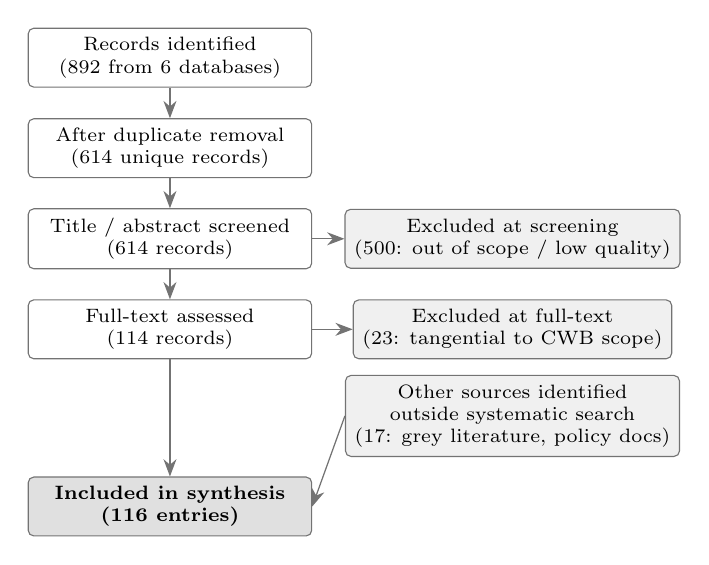
\begin{tikzpicture}[
  prisma/.style={draw=black!55, fill=white, rounded corners=2pt,
    minimum width=3.6cm, minimum height=0.72cm, align=center, font=\scriptsize},
  prismaem/.style={prisma, fill=black!6, minimum width=3.0cm, minimum height=0.58cm},
  arr/.style={-{Stealth[length=2.2mm]}, line width=0.45pt, draw=black!55}
]
  \node[prisma] (id) at (0,0) {Records identified\\(892 from 6 databases)};
  \node[prisma] (dedup) at (0,-1.15) {After duplicate removal\\(614 unique records)};
  \node[prisma] (screen) at (0,-2.3) {Title / abstract screened\\(614 records)};
  \node[prismaem] (excl1) at (4.35,-2.3) {Excluded at screening\\(500: out of scope / low quality)};
  \node[prisma] (full) at (0,-3.45) {Full-text assessed\\(114 records)};
  \node[prismaem] (excl2) at (4.35,-3.45) {Excluded at full-text\\(23: tangential to CWB scope)};
  \node[prismaem] (other) at (4.35,-4.55) {Other sources identified\\outside systematic search\\(17: grey literature, policy docs)};
  \node[prisma, fill=black!12, font=\scriptsize\bfseries] (incl) at (0,-5.7)
    {Included in synthesis\\(116 entries)};
  \draw[arr] (id) -- (dedup);
  \draw[arr] (dedup) -- (screen);
  \draw[arr] (screen) -- (full);
  \draw[arr] (full) -- (incl);
  \draw[arr] (other.west) -- (incl.east);
  \draw[arr] (screen.east) -- (excl1.west);
  \draw[arr] (full.east) -- (excl2.west);
\end{tikzpicture}
\caption[PRISMA-style literature screening flow]{PRISMA-style literature screening flow}
\label{fig:prisma-flow}
\end{figure}

\section{Review of Existing Research}

Each subsection below links prior work to a CWB design choice or research gap.

\subsection{DeFi Lending and the Structural Gap}

Werner et al.~[1] show that DeFi lending is flat, pool-based, and over-collateralized---with no institutional hierarchy. This is the gap Contribution~1 addresses. Bastankhah et al.~[2] support dynamic rate models over static Aave/Compound curves, validating CWB's kinked-rate design (Section~\ref{sec:kinked-rate}). Aspris and Svec~[117] describe modular risk curators but not four-tier development finance. Yang and Cui~[46] and Dao et al.~[59] provide evaluation frameworks for utilization, liquidation, and credit limits in DeFi.

\subsection{Fraud Detection and Explainable AI}
\label{sec:lit-ml-oracle}

Palaiokrassas et al.~[3] show behavioral features raise fraud F1 to 0.76--0.85 on multichain DeFi data---informing CWB's Random Forest plan. BCCC-DeFiFraudTrans-2025~[107] is the target training set (York access request submitted). Liu et al.~[6] motivate Isolation Forest for unlabeled anomaly detection. Caldarelli~(2025)~[122] notes ML-score oracles for lending remain under-researched---supporting Contribution~3.

Adom et al.~[4] favor SHAP over LIME for stable loan explanations; Yuan~[55] shows SHAP credit models above 0.92 AUC. These inform the Authority Brief dashboard for approvers.

\subsection{Hierarchical Capital Distribution}
\label{sec:lit-cross-tier}

Tan~[5] and BIS CBDC work~[52, 133, 134] describe two-tier central-bank-to-bank-to-user distribution---parallel to CWB's four tiers. Bindseil~[132] supports asymmetric upward/downward rate spreads for \texttt{UpwardDepositFacility}. Project Pine~[130] and Dong et al.~[131] validate layered smart-contract factories and cross-tier capital flows in policy research, but no single DeFi spec combines them---the gap in Figure~\ref{fig:cross-tier-lending}.

\subsection{Group Lending and Microfinance}

Grameen and BRAC show solidarity groups can repay above 95\% without individual collateral, using weekly meetings and field officers that on-chain systems cannot replicate. CWB's \texttt{GroupLendingPool} encodes mutual liability in code with conservative default assumptions. Asaduzzaman et al.~[53] report up to 60\% admin savings from smart-contract microcredit. A 2025 IEEE microloan prototype~[155] is the closest technical analogue. Jaffer~[118] and Sherratt~[119] warn that mutual liability can become coercive off-chain---a risk CWB avoids but at the cost of weaker social monitoring.

\subsection{Smart Contract Security and Governance}

Atzei et al.~[7] define core EVM attack classes (reentrancy, access control), informing \texttt{ReentrancyGuard} and RBAC. Chaliasos et al.~[149] find tools prevented only 8\% of real exploit losses---motivating a layered Slither--Mythril--Foundry--Tenderly pipeline (Section~\ref{sec:defense-in-depth}). Flash-loan governance attacks (Beanstalk, \$182M)~[157] drive CWB's timelock and snapshot voting. MEV risk on liquidations is mitigated via commit--reveal triggers.

\subsection{Supporting Infrastructure}
\label{sec:lit-stablecoin-reg}
\label{sec:lit-sbt}
\label{sec:lit-institutional}

MiCA~[96, 97] and the GENIUS Act~[98] require stablecoin reserves and issuer authorization---supporting USDC-first retail lending (Section~\ref{sec:stablecoin-first}). Beniiche~[61] and Pasdar~[62] frame the oracle problem; Chainlink accuracy varies by chain~[156], supporting single-chain deployment with commit--reveal fallback.

BIS/FSB data~[20, 24, 32] document correspondent-banking delays and costs. Kim and Kim~[54] and Hartmann and Hasan~[47] inform gas-cost modeling. Buterin et al.~[161] and MicroSave~[91] motivate on-chain credit passports (Section~\ref{sec:credit-passport}). Ozili~[160] shows Nigeria's eNaira had 98.5\% wallet inactivity---barriers are trust-based, supporting MFI-led onboarding. Sygnum~[81], mBridge~[99], FundsChain~[38], and Kinexys~[39] show institutional blockchain adoption without retail lending hierarchies.

\subsection{Zero-Knowledge Proofs for Compliance-Aware DeFi Identity}
\label{sec:lit-zkp-defi}

Recent ACM papers~[152, 153] and Piper et al.~[68] show ZKP + DID/VC can enable privacy-preserving KYC. Together with zkAML~[69], this motivates Contribution~4, deferred past MVT (Section~\ref{sec:future-work}).

\subsection{Future Research Directions Scoped}
\label{sec:lit-gnn}
\label{sec:lit-fl}
\label{sec:lit-retail-payments}
\label{sec:lit-llm}
\label{sec:harness-lit}

GNN-based fraud detection~[84, 85, 120], federated learning across banks~[48, 87, 124], retail payment rails~[135--144], and LLM agent risks (hallucination, prompt injection)~[88, 113--115] are documented in the literature but scoped to Future Work. The MVT agent uses scanning middleware and a human confirmation gate (Section~\ref{sec:optional-agent}).

\section{Summary of Key Findings}
\label{sec:comparative-protocol}

Table~\ref{tab:lit-summary} lists the fifteen highest-impact sources and how each maps to a CWB design decision. Table~\ref{tab:protocol-comparison} compares CWB to major DeFi protocols. Together they support the compound gap claim for RQ1--RQ3.

\begin{table}[H]
\centering
\footnotesize
\setlength{\tabcolsep}{4pt}
\renewcommand{\arraystretch}{1.12}
\caption[Tier-1 literature synthesis]{Tier-1 literature synthesis: core findings and design decisions.}
\label{tab:lit-summary}
\resizebox{\textwidth}{!}{%
\begin{tabular}{@{}>{\raggedright\arraybackslash}p{2.8cm}>{\raggedright\arraybackslash}p{3.6cm}>{\raggedright\arraybackslash}p{3.8cm}>{\raggedright\arraybackslash}p{2.2cm}@{}}
\toprule
\tableheadcolor
\tableheadfont Author \& Year & \tableheadfont Core Finding & \tableheadfont Design Decision & \tableheadfont Phase \\
\midrule
Werner et al.\ 2022 [1] & DeFi lending uniformly flat, pool-based, overcollateralized; no institutional hierarchy & Four-tier architecture as novel design space & Contribution 1 \\
\rowcolor{RowShade}
Aspris \& Svec 2025 [117] & Modular risk curator is closest prior work; lacks multilateral hierarchy & Boundary of prior work for Contribution 1 & Contribution 1 \\
Tan 2023 [5] & Two-tier CBDC distribution (central bank $\to$ banks $\to$ users) & Four-tier capital flow; client-via-Local-Bank path & Architecture \\
\rowcolor{RowShade}
Project Pine 2025 [130] & Hierarchical smart contract factory for central-bank operations & Layered design for IBLP and SyndicatedLoan & Phase II--III \\
Palaiokrassas et al.\ 2024 [3] & Behavioral features: F1 0.76--0.85 vs.\ 0.08 transactional only & Random Forest feature engineering & Contribution 3 \\
\rowcolor{RowShade}
Liu et al.\ 2008 [6] & Isolation Forest via recursive partitioning; shorter paths = anomalies & Secondary unsupervised model when labels scarce & Contribution 3 \\
Adom et al.\ 2022 [4] & SHAP deeper and more consistent than LIME on loan approval & SHAP as primary explainability method & Contribution 3 \\
\rowcolor{RowShade}
Jaffer [118] / IEEEMicroloan 2025 [155] & Solidarity mechanics + most recent blockchain microloan prototype & GroupLendingPool mutual liability design & Contribution 2 \\
Atzei et al.\ 2017 [7] & Foundational EVM attack taxonomy & ReentrancyGuard, CEI, RBAC, Solidity 0.8.20 & Security \\
\rowcolor{RowShade}
Chaliasos et al.\ 2024 [149] & Tools prevented only 8\% of real-world losses; all reentrancy & Layered pipeline---no single tool sufficient & Security \\
Qin et al.\ [157] & Flash-loan governance passes malicious proposals atomically (\$182M) & Snapshot voting, 48-h timelock, 60\% quorum & Governance \\
\rowcolor{RowShade}
Piper et al.\ 2025 [68] + ZKP-KYC [152, 153] & ZKP + SSI + DID enables privacy-preserving KYC & Groth16 KYC circuit, W3C DID/VC choice & Contribution 4 \\
MiCA [96, 97] + GENIUS [98] & Stablecoin issuers require 1:1 reserves, authorization, audits & USDC-first denomination as regulatory requirement & Denomination \\
\rowcolor{RowShade}
Chainlink accuracy [156] & Polygon high oracle accuracy vs Ethereum/zkSync under volatility & Single-chain Polygon deployment; oracle fallback & Infrastructure \\
Gudgeon et al.\ [63] & Utilization above 90\% causes liquidity crises empirically & Kink point at $U^{*} = 80\%$ in rate model & Rate model \\
\bottomrule
\end{tabular}%
}
\end{table}

\begin{table}[H]
\centering
\footnotesize
\setlength{\tabcolsep}{3pt}
\resizebox{\textwidth}{!}{%
\begin{tabular}{@{}p{3.4cm}*{6}{>{\centering\arraybackslash}p{1.35cm}}@{}}
\toprule
\tableheadcolor
\tableheadfont Feature & \tableheadfont Aave & \tableheadfont Comp. & \tableheadfont Maker & \tableheadfont Maple & \tableheadfont Gfinch & \tableheadfont CWB \\
\midrule
Institutional hierarchy & \tmarkNo{} & \tmarkNo{} & \tmarkNo{} & \tmarkNo{} & \tmarkNo{} & \tmarkPlanned{} \\
\rowcolor{RowShade}
Cross-tier capital flow & \tmarkNo{} & \tmarkNo{} & \tmarkNo{} & \tmarkNo{} & \tmarkNo{} & \tmarkPartial{} \\
Same-tier interbank lending & \tmarkNo{} & \tmarkNo{} & \tmarkNo{} & \tmarkNo{} & \tmarkNo{} & \tmarkPartial{} \\
\rowcolor{RowShade}
Syndicated / co-lending & \tmarkNo{} & \tmarkNo{} & \tmarkNo{} & Part. & Part. & \tmarkPartial{} \\
Upward capital repatriation & \tmarkNo{} & \tmarkNo{} & \tmarkNo{} & \tmarkNo{} & \tmarkNo{} & \tmarkPartial{} \\
\rowcolor{RowShade}
Solidarity group lending & \tmarkNo{} & \tmarkNo{} & \tmarkNo{} & \tmarkNo{} & Part. & \tmarkPlanned{} \\
AI/ML fraud detection & \tmarkNo{} & \tmarkNo{} & \tmarkNo{} & Man. & Man. & \tmarkPlanned{} \\
\rowcolor{RowShade}
SHAP explainability & \tmarkNo{} & \tmarkNo{} & \tmarkNo{} & \tmarkNo{} & \tmarkNo{} & \tmarkPlanned{} \\
ZKP KYC compliance & \tmarkNo{} & \tmarkNo{} & \tmarkNo{} & \tmarkNo{} & \tmarkNo{} & \tmarkPlanned{} \\
\rowcolor{RowShade}
Kinked interest rate curve & \tmarkDone{} & \tmarkDone{} & Gov. & \tmarkDone{} & \tmarkNo{} & \tmarkPartial{} \\
Role-based access control & Part. & Part. & Gov. & \tmarkDone{} & Part. & \tmarkPlanned{} \\
\rowcolor{RowShade}
Institutional / L2 focus & \tmarkNo{} & \tmarkNo{} & \tmarkNo{} & \tmarkDone{} & Part. & \tmarkPlanned{} \\
TVL / Status (2026) & \$26B & \$1.4B & \$10B & \$2.6B & \$680M & Planning \\
\bottomrule
\end{tabular}%
}
\caption[Protocol comparison on eleven architectural dimensions]{Protocol comparison on eleven architectural dimensions. Competitor columns reflect publicly documented protocol capabilities (2026); CWB columns reflect pre-thesis specification status.}
\label{tab:protocol-comparison}
\end{table}

%% CHAPTER 3: SYSTEM ARCHITECTURE AND DESIGN
\chapter{System Architecture and Design}

\section{Prototype Scope}
\label{sec:prototype-scope}

Table~\ref{tab:prototype-scope} records design status only; no public-network deployment at pre-thesis.

\begingroup
\footnotesize
\setlength{\tabcolsep}{3.5pt}
\renewcommand{\arraystretch}{0.88}
\begin{table}[H]
\centering
\caption[Prototype scope and implementation status]{Prototype scope: specification vs.\ planned implementation (pre-thesis design record). \textit{Voice:} \textit{specified} = documented design; \textit{planned} = Phase~I--IV deliverable. Target chain: Polygon Amoy and/or Ethereum Sepolia.}
\label{tab:prototype-scope}
\begin{tabular}{@{}p{7.4cm}p{5.4cm}@{}}
\toprule
\tableheadcolor
\tableheadfont Feature & \tableheadfont Status \\
\midrule
Four-tier role system (RBAC) & \tmarkPartial{} Specified \\
\rowcolor{RowShade}
World Bank Reserve contract (Tier~1) & \tmarkPartial{} Specified (Ph.~I) \\
Tier~2 National Bank contracts & \tmarkPartial{} Specified (Ph.~I) \\
\rowcolor{RowShade}
Tier~3 Local Bank contracts & \tmarkPartial{} Specified (Ph.~I) \\
Cross-tier fund transfer & \tmarkPlanned{} Planned (Ph.~II) \\
\rowcolor{RowShade}
Loan request / approval workflow & \tmarkPartial{} Specified (Ph.~II) \\
Installment EMI auto-generation & \tmarkPlanned{} Planned (Ph.~II) \\
\rowcolor{RowShade}
SavingsVault / FixedDeposit contracts & \tmarkPlanned{} Planned (Ph.~II) \\
GroupLendingPool & \tmarkPlanned{} Planned (Ph.~II) \\
\rowcolor{RowShade}
InterBankLendingPool & \tmarkPlanned{} Planned (Ph.~II) \\
AI/ML fraud detection (Random Forest) & \tmarkPlanned{} Planned (Ph.~III) \\
\rowcolor{RowShade}
SHAP + anomaly explainability & \tmarkPlanned{} Planned (Ph.~III) \\
Oracle (Chainlink Functions) & \tmarkPlanned{} Stretch (Ph.~III) \\
\rowcolor{RowShade}
ZKP KYC compliance layer & \tmarkPlanned{} Future Work \\
Testnet deployment (Amoy / Sepolia) & \tmarkPlanned{} Planned (Ph.~IV) \\
\rowcolor{RowShade}
AI Agent / MCP (minimal MVT) & \tmarkPlanned{} Planned (Ph.~III; retail only) \\
Full MCP tool server (17 tools) & \tmarkPlanned{} Future Work \\
\rowcolor{RowShade}
Bank-authority AI agent & \tmarkPlanned{} Future Work \\
EIP-7702 session keys & \tmarkPlanned{} Future Work \\
Authority Brief UI (SHAP) & \tmarkPlanned{} Planned (Ph.~III) \\
\rowcolor{RowShade}
Chainlink Automation / Proof of Reserve & \tmarkPlanned{} Planned (Ph.~I--II) \\
PostgreSQL event listener & \tmarkPlanned{} Planned (Ph.~I--II) \\
\rowcolor{RowShade}
SAR workflow (AML $\to$ freeze) & \tmarkPlanned{} Planned (Ph.~III) \\
\texttt{sessions} / \texttt{agent\_action\_log} schema & \tmarkPartial{} Specified (Ph.~I--III) \\
\rowcolor{RowShade}
300-client Foundry simulation & \tmarkPlanned{} Planned (Ph.~IV) \\
\bottomrule
\end{tabular}
\end{table}
\endgroup

\paragraph{Prototype deployment note.}
\textbf{Prototype implementation target:} Polygon Amoy PoS and/or Ethereum Sepolia (single-chain, stability-first). \textbf{Design preference (comparison only):} Polygon zkEVM offers ZK-validity settlement anchored to Ethereum~L1 and is evaluated in the platform selection tables (Section~\ref{sec:blockchain-fundamentals}, item~E) but is not the default narrative deployment chain in gates, MVT items, or phase deliverables unless explicitly marked as a design reference.

\section{High-Level Architecture}
\label{sec:high-level-arch}

The system employs a \textbf{four-layer decentralised application architecture} (Figure~\ref{fig:three-layer-arch}): a presentation layer (React + wallet integration), a smart-contract layer (fifteen modular EVM contracts centred on the four-tier lending hierarchy), an off-chain services layer (Express REST API, PostgreSQL, FastAPI ML scoring, Chainlink oracle integration, event listener, and Redis cache), and a Chainlink infrastructure layer (Chainlink Functions, Automation, Price Feeds, and Proof of Reserve). A planned Phase~III conversational agent (Qwen3-8B + MCP tool server) attaches to the same API endpoints as the React UI and does not alter on-chain logic. Figure~\ref{fig:component-diagram} elaborates this view with external integrations.

\begin{figure}[H]
\centering
\BalancedDiagram{fig-three-layer-arch}
\caption[Four-layer application architecture]{Four-layer application architecture}
\label{fig:three-layer-arch}
\end{figure}

Figure~\ref{fig:component-diagram} shows component interactions. Core lending contracts are specified in Phase~I; extended modules are planned extensions documented in Appendix~B.

\begin{figure}[H]
\centering
\BalancedDiagram{fig-component-architecture}
\caption[Component diagram (planning phase)]{Component diagram (planning phase)}
\label{fig:component-diagram}
\end{figure}

\begin{table}[H]
\centering
\begin{tabular}{p{3.6cm}p{2.4cm}p{1.8cm}p{6.7cm}}
\toprule
\tableheadcolor
\textbf{Contract} & \textbf{Module} & \textbf{Status} & \textbf{Primary responsibility} \\
\midrule
WorldBankReserve & Tier~1 core & Specified (Phase~I) & Global reserve custody, national-bank registration, downward capital allocation. \\
NationalBank & Tier~2 core & Specified (Phase~I) & Local-bank registration, upward borrowing, downward allocation. \\
LocalBank & Tier~3 core & Specified (Phase~I) & Client onboarding, loan lifecycle, installments, \texttt{freezeAccount}. \\
SavingsVault & Deposits & Specified (Phase~II) & Variable-yield savings, reserve-gated withdrawals. \\
FixedDeposit & Deposits & Specified (Phase~II) & Term deposits with deterministic early-withdrawal penalty. \\
GroupLendingPool & Group credit & Specified (Phase~II) & Solidarity-group formation, consent, mutual liability. \\
FXModule & Treasury / FX & Specified (Phase~II) & Oracle-priced retail FX with disclosed spread. \\
InsuranceFund & Risk buffer & Specified (Phase~II) & Default coverage buffer; Chainlink Proof of Reserve. \\
CurrentAccount & Payments & Specified (Phase~II) & Transactional accounts and atomic peer transfers. \\
InterBankLendingPool & Multi-entity & Specified (Phase~II) & Same-tier interbank liquidity pools per tier. \\
UpwardDepositFacility & Multi-entity & Specified (Phase~II) & Upward surplus repatriation with yield spread. \\
SyndicatedLoan & Multi-entity & Planned (Phase~III) & Multi-lender syndicate consent and disbursement. \\
TranchedPool & Multi-entity & Planned (Phase~III) & Senior/junior tranching and waterfall recovery. \\
TreasurySwap & Multi-entity & Specified (Phase~II) & Institutional oracle-priced asset swaps. \\
NettingEngine & Multi-entity & Future Work & ERD stubs only; Section~\ref{sec:future-work} \\
\bottomrule
\end{tabular}
\TableScreenshotEnd{Smart Contract Inventory: Fifteen Modular Contracts Across Core, Product, and Multi-Entity Modules}
\end{table}

\section{Blockchain Platform Selection}

\begin{figure}[H]
\centering
\ThesisIncludeGraphics[width=\linewidth]{fig-blockchain-stack}
\caption[Layered blockchain and application stack]{Layered blockchain and application stack}
\label{fig:blockchain-stack}
\end{figure}


\begin{table}[H]
\centering
\caption[Blockchain platform selection criteria and justification]{Blockchain platform selection criteria and justification.}
\label{tab:blockchain-selection}
\begin{tabular}{p{3.5cm}p{3.5cm}p{6.5cm}}
\toprule
\tableheadcolor
\textbf{Criterion} & \textbf{Selection} & \textbf{Justification} \\
\midrule
Platform & Ethereum Virtual Machine (EVM) & Largest EVM ecosystem; mature tooling. \\
Network & Polygon Amoy PoS and/or Ethereum Sepolia (prototype implementation) & Free public testnets; zkEVM evaluated, not default prototype chain. \\
Consensus & Public-testnet consensus (PoS/L1 testnet) & Stable testnet consensus; ZK settlement is a design preference only. \\
Smart contract language & Solidity 0.8.20 & Industry standard; overflow-safe compiler; rich libraries. \\
\bottomrule
\end{tabular}
\TableScreenshotEnd{Blockchain Platform Selection: Comparison of EVM-Compatible Networks}
\end{table}

\vspace{2pt}
\noindent\textit{\small This platform selection table compares candidate networks on cost, finality, throughput, and ecosystem maturity. Polygon zkEVM remains a design preference for ZK-anchored settlement, but the prototype implementation target is Amoy/Sepolia for stability-first delivery within the thesis timeline.}

\begin{table}[H]
\centering
\caption[Blockchain platform selection (continued)]{Blockchain platform selection (continued): operational and deployment factors.}
\begin{tabular}{p{3.5cm}p{3.5cm}p{6.5cm}}
\toprule
\tableheadcolor
\textbf{Criterion} & \textbf{Selection} & \textbf{Justification} \\
\midrule
Gas cost & \$0.001--\$0.01 per transaction & Far below mainnet; viable for micro-loans. \\
Block finality & $\approx$2 seconds & Fast retail UX; L1-anchored security. \\
Developer tooling & Hardhat + OpenZeppelin & Hardhat tests; audited OpenZeppelin libs. \\
Testnet availability & Amoy (Polygon PoS), Sepolia (Ethereum) & Free faucets; EVM-identical; no real funds. \\
Security model & Public-testnet security model & Testnet PoS; ZK settlement evaluated separately. \\
Migration path & EVM-compatible & Portable Solidity across EVM chains. \\
\bottomrule
\end{tabular}
\TableScreenshotEnd{Blockchain Platform Selection (Continued): Operational and Deployment Factors}
\end{table}

\vspace{2pt}
\noindent\textit{\small This supplementary comparison expands the platform evaluation to additional operational and deployment factors. The conclusion is that Polygon zkEVM Cardona provides a practical balance of ZK-secured settlement and low transaction costs for an academic prototype, with a clear migration path if future requirements demand alternative L2s.}

\subsection{Transaction Verification and Consensus}

\begin{itemize}[noitemsep]
\item \textbf{Polygon zkEVM Cardona:} ZK validity proofs anchor batches to Ethereum~L1 (cryptographic security vs.\ PoS validator assumption on Amoy).
\item \textbf{On prototype testnets:} Amoy and Sepolia provide free public testnets for incremental development and testing without exposure to real-asset risk.
\end{itemize}

\paragraph{Gas-cost sustainability.}
The hierarchical loan lifecycle generates multiple on-chain state transitions per client; on Polygon zkEVM Cardona the \textbf{projected} cost remains well below 0.01\% of interest earned on a representative retail loan (Section~\ref{sec:gas-cost}), to be validated by the Phase~IV Foundry simulation. This margin underpins the micro-loan economics that motivate Layer~2 deployment in the platform selection above.

\subsection{Oracle Architecture: Off-Chain AI to On-Chain Decision}
\label{sec:oracle-architecture}

The Crypto World Bank requires a mechanism to convey off-chain AI/ML risk assessments into the on-chain loan approval workflow. This is an instance of the oracle problem~[61, 62]. The graded MVT oracle path is \textbf{commit--reveal}, with Chainlink Functions retained as a stretch upgrade when supported on the chosen testnet.

\paragraph{Commit-reveal relay (MVT oracle path).}
Phases~I--III use a \textbf{commit--reveal relay} as the primary oracle mechanism for ML risk scores. The off-chain ML service commits a hash $h = \text{keccak256}(s \,\|\, \text{nonce})$ to the \texttt{LoanController} contract, then reveals $s$ and the nonce within the decision window. The contract verifies $h = \text{keccak256}(s \,\|\, \text{nonce})$ and stores $s$ immutably. This pattern prevents score manipulation between commitment and decision and creates an immutable on-chain audit trail of every risk score used in a lending decision. A centralized relay (trusted backend calling \texttt{updateRiskScore}) remains a Phase~I--II integration aid only.

\paragraph{Chainlink Functions oracle (stretch / future work).}
\textbf{Chainlink Functions} is documented as a production-grade upgrade path when DON support is available on the chosen testnet. Chainlink Functions operates via a Decentralised Oracle Network (DON): the ML risk score is fetched independently by multiple Chainlink nodes, consensus across the DON is required before the result is committed on-chain, and no single compromised node can manipulate the risk score. The source code executed by the DON is:

\begin{verbatim}
// Chainlink Functions source (runs in decentralised DON)
const clientId = args[0];
const response = await Functions.makeHttpRequest({
  url: `https://your-ml-service.com/score/${clientId}`,
  method: "POST"
});
const score = response.data.risk_score;
// 6 decimal precision
return Functions.encodeUint256(Math.round(score * 1e6));
\end{verbatim}

The DON adds 30--60 seconds of latency and \$0.10--\$1.00 per oracle call, both acceptable for the loan approval lifecycle where decisions are not time-critical. At MVT scope, commit--reveal remains authoritative; Chainlink Functions is a \textbf{stretch} deliverable (DT-III.01, Should) when supported on Amoy/Sepolia.

\paragraph{Chainlink Automation: installment triggers (automation upgrade path).}
\textbf{Chainlink Automation} replaces the centralised cron job for overdue installment detection and interest accrual. The entire loan lifecycle from application to overdue flagging runs without a trusted operator:

\begin{verbatim}
// In LocalBankPool.sol
function checkUpkeep(bytes calldata) external view override
    returns (bool upkeepNeeded, bytes memory performData) {
    uint256[] memory overdueLoans = getOverdueLoans();
    upkeepNeeded = overdueLoans.length > 0;
    performData = abi.encode(overdueLoans);
}

function performUpkeep(bytes calldata performData) external override {
    uint256[] memory overdueLoans =
        abi.decode(performData, (uint256[]));
    for (uint i = 0; i < overdueLoans.length; i++) {
        _markInstallmentOverdue(overdueLoans[i]);
    }
}
\end{verbatim}

This reduces reliance on unilateral off-chain cron execution for overdue detection by making installment-trigger checks externally verifiable through an on-chain upkeep interface. The broader system still includes licensed/operator-controlled off-chain services for KYC and risk analytics (Section~\ref{sec:blockchain-fundamentals}).

\paragraph{Chainlink Price Feeds: fiat and crypto pairs.}
The \texttt{FXModule} contract uses Chainlink's production-grade \texttt{AggregatorV3Interface} price feeds for ETH/USD, USDC/USD, and governance-selected fiat pairs (e.g.\ EUR/USD), replacing the earlier ``forex oracle approved by governance'' pattern. Optional fiat-equivalent display in the frontend flows through:

\begin{verbatim}
// In LocalBankPool.sol
AggregatorV3Interface internal fiatUsdFeed;  // e.g. EUR/USD
AggregatorV3Interface internal ethUsdFeed;

function getFiatEquivalent(uint256 usdcAmount)
    public view returns (uint256) {
    (, int fiatRate,,,) = fiatUsdFeed.latestRoundData();
    // USDC tracks USD 1:1; Chainlink uses 8 decimals
    return usdcAmount * uint256(fiatRate) / 1e8;
}
\end{verbatim}

The 8-decimal precision convention is the Chainlink standard for fiat-pair feeds. Chainlink price feeds are a planned Phase~I integration for optional fiat-equivalent display in the frontend.

\paragraph{Chainlink Proof of Reserve.}
The \texttt{WorldBankReserve} contract publishes its reserve balance to \textbf{Chainlink Proof of Reserve (PoR)}, making the reserve cryptographically verifiable by any external auditor without trusting CWB's administrator. This is the ``free PoR'' advantage over FTX: any external system can verify reserve solvency without relying on CWB's admin claims.

\begin{verbatim}
// WorldBankReserve.sol
function getReserveSummary() external view returns (
    uint256 totalDeposited,
    uint256 totalLoaned,
    uint256 reserveRatio,   // scaled 1e4 (e.g. 5000 = 50%)
    uint256 insuranceFundBalance
) {
    return (
        totalDeposited,
        totalLoaned,
        (totalDeposited - totalLoaned) * 1e4 / totalDeposited,
        insuranceFund.balance()
    );
}
\end{verbatim}

This function is the FTX commingling safeguard described in Section~\ref{sec:defense-in-depth}. Adding Chainlink's PoR job on top turns it into a market-standard verifiable proof, and it is specified in full in Appendix~D.

\begin{figure}[H]
\centering
\BalancedDiagram{fig-oracle-architecture}
\caption[Oracle architecture]{Oracle architecture}
\label{fig:oracle-architecture}
\end{figure}


\section{Data Model and Database Design}
\label{sec:data-model}

The relational database schema comprises 51 normalized entities in Third Normal Form (3NF): 31 core prototype entities (Table~\ref{tab:db-entities}), six primary extension entities (Table~\ref{tab:db-entities-ext}), and 14 Phase~II--III banking-product and multi-entity entity stubs (Table~\ref{tab:db-entities-ext2}). Core entities are Phase~I MVT-complete specifications; stub entities carry PK, FK anchors, and one-sentence roles in Table~\ref{tab:db-entities-ext2} and are fully attribute-specified in Section~\ref{sec:multi-entity}. Figure~\ref{fig:core-system-graph} presents the core entity-relationship overview, Figure~\ref{fig:erd-extended} presents extended product and multi-entity entities, and Figure~\ref{fig:eer} presents the Enhanced Entity-Relationship (EER) diagram with specialisation and weak-entity constructs.

\begin{figure}[H]
\centering
\BalancedDiagram{fig-erd-core}
\caption[Core system entity graph]{Core system entity graph}
\label{fig:core-system-graph}
\end{figure}

\begin{figure}[H]
\centering
\BalancedDiagram{fig-erd-extended}
\caption[Extended ERD: banking products]{Extended ERD: banking-product entities (crow's-foot; PK shown, full attributes in Table~\ref{tab:db-entities-ext2}).}
\label{fig:erd-extended}
\end{figure}

\begin{landscape}
\begin{figure}[p]
\centering
\ThesisIncludeGraphics[width=\linewidth,height=0.82\textheight,keepaspectratio]{fig-erd-multientity}
\caption[Extended ERD: multi-entity operations]{Extended ERD: multi-entity and cross-tier operational entities (crow's-foot; PK shown, full attributes in Table~\ref{tab:db-entities-ext2}).}
\label{fig:erd-multientity}
\end{figure}
\end{landscape}

The current ERD covers the core lending and governance entities. Figure~\ref{fig:erd-extended} presents the extended banking-product entities (SavingsAccount, FixedDeposit, LoanGroup, GroupMember, CurrentAccount, and InsuranceFund), and Figure~\ref{fig:erd-multientity} presents the multi-entity / cross-tier operational entities described in Section~\ref{sec:multi-entity-consistency}: \texttt{INTERBANK\_LOAN}, \texttt{UPWARD\_DEPOSIT}, \texttt{SYNDICATE} and \texttt{SYNDICATE\_MEMBER}, \texttt{TRANCHED\_POOL}, \texttt{TREASURY\_SWAP}, and \texttt{NETTING\_BATCH} with \texttt{NETTING\_ENTRY}. Their foreign-key relationships into the core lending entities (LOAN, BANK\_USER, INSTALLMENT, TRANSACTION) are detailed in Table~\ref{tab:ext-entity-fks} in Section~\ref{sec:multi-entity-consistency}. The data model remains in one-to-one consistency with the contract architecture and implementation phase plan.


\begin{figure}[H]
\centering
\BalancedDiagram{fig-eer-model}
\caption[Enhanced EER model]{Enhanced EER model}
\label{fig:eer}
\end{figure}

\clearpage
\subsection{Entity Summary}

\begin{table}[H]
\centering
\caption[Database entity summary (31 core entities)]{Database entity summary (31 core entities): primary keys and roles.}
\label{tab:db-entities}
\small
\begin{tabular}{@{}p{2.6cm}p{3.4cm}p{7.0cm}@{}}
\toprule
\tableheadcolor
\textbf{Entity} & \textbf{Primary key} & \textbf{Role / Description} \\
\midrule
INSTITUTION & \texttt{institution\_id} & Shared supertype for all banking-tier identities. Attributes: \texttt{institution\_type} \texttt{ENUM('WORLD','NATIONAL','LOCAL')}, \texttt{name}, \texttt{wallet\_address}, \texttt{contract\_address}, \texttt{status}, \texttt{created\_at}. All multi-entity tables (\texttt{INTERBANK\_LOAN}, \texttt{NETTING\_ENTRY}, \ldots) reference this PK for enforceable cross-tier FKs. \\
COUNTRY & \texttt{country\_code} & ISO~3166-1 alpha-2 reference (PK). Attributes: \texttt{name}, \texttt{default\_stablecoin\_symbol}, \texttt{regulatory\_regime\_tag}. \\
WORLD\_BANK & \texttt{institution\_id} & Subtype of \texttt{INSTITUTION} (\texttt{institution\_type='WORLD'}); PK is also FK $\to$ \texttt{INSTITUTION}. Singleton enforced: \texttt{CHECK (institution\_id = 1)} plus no-delete trigger. Global reserve parameters; on-chain binding: \texttt{chain\_id}, \texttt{last\_synced\_block}, \texttt{deployment\_tx\_hash}. \\
NATIONAL\_BANK & \texttt{institution\_id} & Subtype of \texttt{INSTITUTION} (\texttt{institution\_type='NATIONAL'}); FK \texttt{country\_code} $\to$ \texttt{COUNTRY} with \texttt{UNIQUE} (one national reserve per nation). FK \texttt{parent\_world\_bank\_id} $\to$ \texttt{WORLD\_BANK}. \\
LOCAL\_BANK & \texttt{institution\_id} & Subtype of \texttt{INSTITUTION} (\texttt{institution\_type='LOCAL'}); FK \texttt{national\_bank\_id} $\to$ \texttt{NATIONAL\_BANK}. City-level banks lending to retail clients. \\
BANK\_USER & \texttt{bank\_user\_id} & Bank staff with role-based permissions. \texttt{bank\_type} \texttt{ENUM('world','national','local')}; nullable FKs \texttt{world\_bank\_id}, \texttt{national\_bank\_id}, \texttt{local\_bank\_id} with CHECK enforcing exactly one parent institution (Table~\ref{tab:integrity-constraints}). \\
BORROWER & \texttt{borrower\_id} & End borrowers (UK: \texttt{wallet\_address}). FK \texttt{registered\_local\_bank\_id} $\to$ \texttt{LOCAL\_BANK} (NOT NULL, set at onboarding) records the client's home Local Bank for KYC attribution and dashboard scoping; \texttt{LOAN\_REQUEST} remains the separate M:N association for banks at which the client has applied.\footnote{The prototype uses \texttt{BORROWER} / \texttt{borrower\_id} consistently; the final migration may rename to \texttt{CLIENT} / \texttt{client\_id}. The \texttt{UNIQUE} constraint on \texttt{wallet\_address} assumes single-chain operation on Polygon zkEVM Cardona (Section~\ref{sec:bridge}).} \\
LOAN\_REQUEST & \texttt{request\_id} & Loan applications and approval workflow. \texttt{status} (lifecycle): \texttt{DRAFT}, \texttt{SUBMITTED}, \texttt{UNDER\_REVIEW}, \texttt{APPROVED}, \texttt{REJECTED}, \texttt{DISBURSED}, \texttt{CANCELLED}. \texttt{oracle\_state} (event-listener only): \texttt{NONE}, \texttt{COMMIT\_PENDING}, \texttt{COMMITTED}, \texttt{DON\_REQUESTED}, \texttt{SCORE\_REVEALED}. FKs: \texttt{submission\_event\_log\_id}, \texttt{approval\_event\_log\_id}; \texttt{on\_chain\_request\_id}. \\
LOAN & \texttt{loan\_id} & Active loan after disbursement; FK \texttt{loan\_request\_id} $\to$ \texttt{LOAN\_REQUEST}; collateral and loan asset references. \texttt{on\_chain\_loan\_id}, \texttt{disbursement\_event\_log\_id}. \\
INSTALLMENT & \texttt{loan\_id}, \texttt{installment\_number} & Repayment schedule (weak entity on \texttt{LOAN}; composite PK). \texttt{payment\_event\_log\_id}, \texttt{payment\_tx\_hash}. \\
TRANSACTION & \texttt{transaction\_id} & Financial ledger records for retail and institutional flows. \texttt{transaction\_type} (\texttt{LOAN\_DISBURSEMENT}, \texttt{INSTALLMENT\_PAYMENT}, \texttt{INTERBANK\_TRANSFER}, \texttt{UPWARD\_DEPOSIT}, \texttt{TREASURY\_SWAP}, \ldots), \texttt{direction} (\texttt{CREDIT}/\texttt{DEBIT}). Nullable FKs: \texttt{borrower\_id} $\to$ \texttt{BORROWER} (retail flows); \texttt{origin\_institution\_id}, \texttt{counterparty\_institution\_id} $\to$ \texttt{INSTITUTION} (institution-to-institution flows). CHECK: at least one actor side is non-null. \texttt{blockchain\_tx\_hash}, \texttt{event\_log\_id}. \\
BORROWING\_LIMIT & \texttt{limit\_id} & Per-borrower limits with 6-month and 1-year rolling windows (UK: \texttt{borrower\_id}). \texttt{last\_computed\_at}, \texttt{last\_synced\_block}, \texttt{on\_chain\_enforced\_limit}, \texttt{sync\_discrepancy\_flag}. Authoritative enforcement remains on-chain. \\
CREDIT\_PASSPORT & \texttt{passport\_id} & Read-model projection of on-chain CreditPassport SBT events (event-listener owned). FK \texttt{borrower\_id}; \texttt{wallet\_address}, \texttt{on\_chain\_token\_id}, \texttt{credit\_score}, \texttt{risk\_tier}, \texttt{open\_loans}, \texttt{total\_defaults}, \texttt{kyc\_level}, \texttt{last\_score\_updated\_at}, \texttt{last\_updated\_block}, \texttt{chain\_id}. \\
\bottomrule
\end{tabular}
\TableScreenshotEnd{Database Entity Summary (Part A): Core Lending and Client Entities}
\end{table}

\newpage
\begin{table}[H]
\centering
\caption[Database entity summary (continued)]{Database entity summary (continued): auxiliary, analytics, and profile entities.}
\small
\begin{tabular}{@{}p{2.6cm}p{3.4cm}p{7.0cm}@{}}
\toprule
\tableheadcolor
\textbf{Entity} & \textbf{Primary key} & \textbf{Role / Description} \\
\midrule
INCOME\_PROOF & \texttt{proof\_id} & Income verification documents (multi-valued per borrower). \\
CHAT\_MESSAGE & \texttt{message\_id} & Human-to-human client$\leftrightarrow$bank messages in the loan workflow. FK to \texttt{LOAN\_REQUEST} and/or \texttt{LOAN}. Not agent-specific; not for inter-tier authority communication (see \texttt{INSTITUTION\_MESSAGE}). \\
INSTITUTION\_MESSAGE & \texttt{message\_id} & Cross-tier / cross-authority communication audit trail. FK \texttt{sender\_institution\_id}, \texttt{receiver\_institution\_id} $\to$ \texttt{INSTITUTION}; \texttt{message\_type} (\texttt{SAR\_ESCALATION}, \texttt{SYNDICATION\_INVITE}, \texttt{RESERVE\_ALERT}, \texttt{IBLP\_REQUEST}, \ldots), \texttt{payload} (JSONB), \texttt{status}, \texttt{created\_at}, \texttt{read\_at}. \\
AGENT\_CONVERSATION\_TURN & \texttt{turn\_id} & Each turn of the Qwen3-8B agent conversation (Phase~III). FK \texttt{session\_id} $\to$ \texttt{SESSIONS}. Stores \texttt{role} (user/assistant/system), \texttt{content\_summary}, \texttt{tokens\_used}, \texttt{tool\_calls} (JSONB). Separate from \texttt{AGENT\_ACTION\_LOG} (write-tool execution only). \\
MODEL\_REGISTRY & \texttt{model\_id} & ML model lineage for audit and explainability. Attributes: \texttt{model\_name}, \texttt{version}, \texttt{training\_date}, \texttt{metrics} (JSONB), \texttt{artifact\_hash}, \texttt{is\_active}. Referenced by \texttt{LOAN\_RISK\_ASSESSMENT}. \\
LOAN\_RISK\_ASSESSMENT & \texttt{assessment\_id} & Per-loan ML inference record: FK \texttt{loan\_request\_id} $\to$ \texttt{LOAN\_REQUEST}; FK \texttt{model\_id} $\to$ \texttt{MODEL\_REGISTRY}; \texttt{fraud\_probability}, \texttt{anomaly\_score}, \texttt{shap\_vector} (JSONB), \texttt{feature\_vector\_hash}, \texttt{created\_at}. \\
SECURITY\_EVENT\_LOG & \texttt{event\_id} & System-wide security and AML events (append-only). Attributes: \texttt{event\_type}, \texttt{actor\_id}, \texttt{actor\_type}, \texttt{severity}, \texttt{payload} (JSONB), \texttt{created\_at}. INSERT-only RLS policy; distinct from per-loan \texttt{LOAN\_RISK\_ASSESSMENT}. \\
MARKET\_DATA & \texttt{market\_data\_id} & Non-Chainlink price cache (e.g.\ CoinGecko fallback). Read-only auxiliary; no FK into core lending. Key attributes: \texttt{symbol}, \texttt{price\_usd}, \texttt{source}, \texttt{recorded\_at}. Chainlink rounds are stored in \texttt{CHAINLINK\_PRICE\_ROUND}. \\
CHAINLINK\_PRICE\_ROUND & \texttt{round\_id} & Chainlink \texttt{AggregatorV3Interface} round cache: \texttt{feed\_address}, \texttt{pair\_symbol}, \texttt{answer}, \texttt{round\_id\_on\_chain}, \texttt{answered\_in\_round}, \texttt{updated\_at}, \texttt{chain\_id}. Required for staleness check (\texttt{answeredInRound} $<$ \texttt{roundId}). \\
PROFILE\_SETTING & \texttt{profile\_id} & Interface preferences for borrowers and bank staff. Nullable FKs: \texttt{borrower\_id} $\to$ \texttt{BORROWER}; \texttt{bank\_user\_id} $\to$ \texttt{BANK\_USER}. CHECK: exactly one FK is non-null. Attributes: \texttt{language\_setting}, \texttt{display\_currency}, \texttt{notification\_enabled}. \\
CREDIT\_PASSPORT\_HISTORY & \texttt{history\_id} & Append-only audit trail of \texttt{CREDIT\_PASSPORT} score and tier changes (event-listener owned). \\
COLLATERAL\_POSITION & \texttt{position\_id} & Event-listener-owned projection of on-chain collateral lock state. FK \texttt{borrower\_id} $\to$ \texttt{BORROWER}; FK \texttt{loan\_id} $\to$ \texttt{LOAN}; FK \texttt{asset\_id} $\to$ \texttt{ASSETS}. Attributes: \texttt{locked\_amount}, \texttt{lock\_tx\_hash}, \texttt{liquidation\_threshold}, \texttt{last\_synced\_block}, \texttt{chain\_id}. READ-ONLY for Express API; written exclusively by event listener (RLS enforced). \\
BLOCKCHAIN\_EVENT\_LOG & \texttt{event\_id} & Canonical off-chain cache of on-chain event receipts. Populated exclusively by the event listener. Attributes: \texttt{contract\_address}, \texttt{event\_name}, \texttt{tx\_hash} (UNIQUE), \texttt{block\_number}, \texttt{log\_index}, \texttt{chain\_id}, \texttt{raw\_data} (JSONB), \texttt{recorded\_at}. Referenced by FK from \texttt{LOAN\_REQUEST}, \texttt{LOAN}, and \texttt{INSTALLMENT} for audit linkage. \\
AUDIT\_LOGS & \texttt{audit\_id} & General-purpose append-only event log for governance and compliance events not covered by \texttt{AGENT\_ACTION\_LOG}. Attributes: \texttt{event\_type}, \texttt{actor\_id}, \texttt{actor\_type}, \texttt{payload} (JSONB), \texttt{created\_at}. INSERT-only RLS policy. \\
\bottomrule
\end{tabular}
\end{table}

\newpage
\begin{table}[H]
\centering
\caption[Database entity summary (continued)]{Database entity summary (continued): agent session and reference entities.}
\small
\setlength{\tabcolsep}{4pt}
\renewcommand{\arraystretch}{1.08}
\begin{tabular}{@{}>{\raggedright\arraybackslash}p{3.1cm}>{\raggedright\arraybackslash}p{2.7cm}>{\raggedright\arraybackslash}p{7.0cm}@{}}
\toprule
\tableheadcolor
\textbf{Entity} & \textbf{Primary key} & \textbf{Role / Description} \\
\midrule
SESSIONS & \texttt{session\_id} & Wallet session registry for the \textbf{retail-client} conversational agent (Phase~III Must): FK \texttt{borrower\_id} $\to$ \texttt{BORROWER}; device/IP hash, EIP-7702 session-key scope and TTL, parent lineage, compression summary, end reason. Bank-authority agent sessions (\texttt{actor\_type='BANK\_USER'}) are Future Work (Section~\ref{sec:prototype-scope}). Phase~II: \texttt{SESSION\_ANCESTOR} closure table (Section~\ref{sec:integrity-constraints}). \\
AGENT\_ACTION\_LOG & \texttt{action\_id} & Append-only agent write-tool log (\texttt{session\_id}, \texttt{tool\_name}, \texttt{parameters}, \texttt{confirmation\_turn\_id}, \texttt{onchain\_tx\_hash}, \texttt{status}). Separate from \texttt{AGENT\_CONVERSATION\_TURN}; INSERT-only RLS policy. \\
INTEREST\_RATE\_TIER & \texttt{tier\_id} & Normalised kinked-rate parameters (\texttt{base\_rate}, \texttt{kink\_utilisation}, \texttt{rate\_above\_kink}, \texttt{max\_rate}); Section~\ref{sec:normalization}. Discriminator: \texttt{bank\_tier\_type} \texttt{ENUM('world','national','local')}. Temporal validity: \texttt{effective\_from}, \texttt{effective\_to}, \texttt{governance\_proposal\_id}, \texttt{superseded\_by}, \texttt{is\_active}. Partial unique: \texttt{(bank\_tier\_type) WHERE is\_active = TRUE}. \\
ASSETS & \texttt{asset\_id} & Collateral and loan asset registry (UK: \texttt{symbol}); referenced by \texttt{LOAN} via \texttt{collateral\_asset\_id} and \texttt{loan\_asset\_id}. \\
\bottomrule
\end{tabular}
\TableScreenshotEnd{Database Entity Summary (Part B): Agent Session and Reference Entities}
\end{table}

\vspace{2pt}
\noindent\textit{\small This entity summary table enumerates 31 core relational entities. Key additions beyond the original lending core include the \texttt{INSTITUTION} supertype and \texttt{COUNTRY} reference (shared identity for cross-tier operations), \texttt{INSTITUTION\_MESSAGE} (inter-tier authority communication), split ML tables (\texttt{MODEL\_REGISTRY}, \texttt{LOAN\_RISK\_ASSESSMENT}, \texttt{SECURITY\_EVENT\_LOG}), \texttt{registered\_local\_bank\_id} on \texttt{BORROWER}, and institution-aware \texttt{TRANSACTION} columns. Six extension entities (Table~\ref{tab:db-entities-ext}) and 14 Phase~II--III stubs (Table~\ref{tab:db-entities-ext2}) complete the schema to 51 total.}

\begin{table}[H]
\centering
\caption[Extension entities (Phase II--III)]{Extension entities (Phase II--III): primary keys and roles.}
\label{tab:db-entities-ext}
\small
\begin{tabular}{@{}p{2.8cm}p{3.2cm}p{7.2cm}@{}}
\toprule
\tableheadcolor
\textbf{Entity} & \textbf{Primary key} & \textbf{Role / Description} \\
\midrule
GROUP\_CONSENT & \texttt{consent\_id} & Per-member multi-signature consent for \texttt{GroupLendingPool} (UK: \texttt{loan\_request\_id}, \texttt{member\_id}). \texttt{consent\_tx\_hash}, \texttt{event\_log\_id}. \\
TRANCHED\_POOL\_SUBSCRIPTION & \texttt{subscription\_id} & Investor tranche positions: \texttt{pool\_id}, \texttt{subscriber\_id}, \texttt{subscriber\_type}, \texttt{tranche} (\texttt{SENIOR}/\texttt{JUNIOR}), \texttt{committed\_amount}, \texttt{subscription\_tx\_hash}. \\
NETTING\_COORDINATOR\_STATE & \texttt{batch\_id} & Off-chain Settlement Coordinator state: \texttt{status} (\texttt{COMPUTING} $\to$ \texttt{SETTLED}), \texttt{gross\_obligations}, \texttt{net\_settlements} (JSONB), \texttt{challenge\_deadline}, \texttt{on\_chain\_batch\_id}. \\
KYC\_VERIFICATION\_REQUEST & \texttt{request\_id} & ZKP KYC workflow tracker: \texttt{borrower\_id}, \texttt{kyc\_level\_requested}, \texttt{status}, \texttt{credential\_hash}, \texttt{proof\_hash}, \texttt{on\_chain\_tx\_hash}. \\
ORACLE\_HEARTBEAT\_MONITOR & \texttt{monitor\_id} & Chainlink feed staleness monitor: \texttt{feed\_address}, \texttt{pair\_symbol}, \texttt{expected\_heartbeat\_seconds}, \texttt{last\_round\_id}, \texttt{is\_stale}, \texttt{chain\_id}. \\
SESSION\_ANCESTOR & \texttt{session\_id}, \texttt{ancestor\_id} & Closure table for session lineage (replaces recursive INSERT trigger). \texttt{depth} (1 = direct parent). \\
\bottomrule
\end{tabular}
\TableScreenshotEnd{Extension Entities: Group Consent, Netting, KYC, Oracle, and Session Tables}
\end{table}

\begin{table}[H]
\centering
\caption[Extended banking and multi-entity entity stubs (Phase~II--III)]{Extended banking and multi-entity entity stubs (Phase~II--III).}
\label{tab:db-entities-ext2}
\small
\begin{tabular}{@{}p{3.2cm}p{3.0cm}p{6.5cm}@{}}
\toprule
\tableheadcolor
\textbf{Entity} & \textbf{Primary Key} & \textbf{Role / FK anchors} \\
\midrule
SAVINGS\_ACCOUNT & \texttt{account\_id} & SavingsVault deposit account. FK \texttt{borrower\_id} $\to$ \texttt{BORROWER}; FK \texttt{local\_bank\_id} $\to$ \texttt{LOCAL\_BANK(institution\_id)}. \texttt{on\_chain\_address}, \texttt{balance}, \texttt{last\_synced\_block}. \\
FIXED\_DEPOSIT & \texttt{deposit\_id} & FixedDeposit term product. FK \texttt{borrower\_id}; FK \texttt{local\_bank\_id} $\to$ \texttt{LOCAL\_BANK(institution\_id)}. \texttt{principal}, \texttt{maturity\_date}, \texttt{on\_chain\_address}. \\
CURRENT\_ACCOUNT & \texttt{ca\_id} & Transactional account. FK \texttt{borrower\_id}; FK \texttt{local\_bank\_id} $\to$ \texttt{LOCAL\_BANK(institution\_id)}. \texttt{balance}, \texttt{on\_chain\_address}. \\
LOAN\_GROUP & \texttt{group\_id} & GroupLendingPool on-chain group. FK \texttt{local\_bank\_id} $\to$ \texttt{LOCAL\_BANK(institution\_id)}. \texttt{on\_chain\_group\_id}, \texttt{max\_members}, \texttt{status}. \\
GROUP\_MEMBER & \texttt{member\_id} & Weak entity on \texttt{LOAN\_GROUP}. FK \texttt{group\_id}; FK \texttt{borrower\_id}. \texttt{joined\_at}, \texttt{consent\_tx\_hash}. \\
INSURANCE\_FUND & \texttt{fund\_id} & InsuranceFund reserve tracker. FK \texttt{local\_bank\_id} $\to$ \texttt{LOCAL\_BANK(institution\_id)}. \texttt{balance}, \texttt{on\_chain\_address}, \texttt{last\_synced\_block}. \\
\midrule
INTERBANK\_LOAN & \texttt{ib\_loan\_id} & IBLP same-tier liquidity loan. FK \texttt{lender\_institution\_id}, \texttt{borrower\_institution\_id} $\to$ \texttt{INSTITUTION}; trigger/CHECK enforces matching \texttt{institution\_type} per pool instance (\texttt{IBLP\_NB} or \texttt{IBLP\_LB}). \texttt{tenor\_days}, \texttt{amount}, \texttt{status}, \texttt{on\_chain\_tx\_hash}. \\
UPWARD\_DEPOSIT & \texttt{ud\_id} & UpwardDepositFacility surplus deposit. FK \texttt{depositor\_institution\_id}, \texttt{parent\_institution\_id} $\to$ \texttt{INSTITUTION}; CHECK enforces adjacent tier-pair (Local$\to$National or National$\to$World). \texttt{amount}, \texttt{rate}, \texttt{on\_chain\_tx\_hash}. \\
SYNDICATE & \texttt{syndicate\_id} & SyndicatedLoan deal header. FK \texttt{lead\_institution\_id} $\to$ \texttt{INSTITUTION}; FK \texttt{borrower\_id} $\to$ \texttt{BORROWER}. \texttt{total\_amount}, \texttt{status}, \texttt{on\_chain\_address}. \\
SYNDICATE\_MEMBER & \texttt{syndicate\_id}, \texttt{member\_institution\_id} & Co-lender position. FK \texttt{member\_institution\_id} $\to$ \texttt{INSTITUTION}. \texttt{committed\_amount}, \texttt{share\_bps}, \texttt{consent\_tx\_hash}. \\
TRANCHED\_POOL & \texttt{pool\_id} & TranchedPool deal header. FK \texttt{sponsor\_institution\_id} $\to$ \texttt{INSTITUTION}. \texttt{senior\_target}, \texttt{junior\_target}, \texttt{status}, \texttt{on\_chain\_address}. \\
TREASURY\_SWAP & \texttt{swap\_id} & TreasurySwap record. FK \texttt{initiator\_institution\_id} $\to$ \texttt{INSTITUTION}. \texttt{from\_asset\_id}, \texttt{to\_asset\_id}, \texttt{amount\_from}, \texttt{amount\_to}, \texttt{swap\_tx\_hash}. \\
NETTING\_BATCH & \texttt{batch\_id} & NettingEngine settlement batch header. \texttt{gross\_obligations} (JSONB), \texttt{status}, \texttt{on\_chain\_batch\_id}. \\
NETTING\_ENTRY & \texttt{entry\_id} & Individual net position per institution per batch. FK \texttt{batch\_id} $\to$ \texttt{NETTING\_BATCH}; FK \texttt{participant\_institution\_id} $\to$ \texttt{INSTITUTION}. \texttt{net\_amount}, \texttt{settled\_tx\_hash}. \\
\bottomrule
\end{tabular}
\TableScreenshotEnd{Extended Banking and Multi-Entity Entity Stubs (Phase II--III)}
\end{table}

\vspace{2pt}
\noindent\textit{\small Extended banking entities in Figure~\ref{fig:erd-extended} (\texttt{SAVINGS\_ACCOUNT}, \texttt{FIXED\_DEPOSIT}, \texttt{LOAN\_GROUP}, \ldots) include planned on-chain anchor fields \texttt{on\_chain\_address} and \texttt{last\_synced\_block} so the event listener can map incoming events to the correct DB row. Multi-entity stub FKs anchor to \texttt{INSTITUTION.institution\_id} (Table~\ref{tab:db-entities-ext2}) rather than tier-specific PK namespaces, enabling one enforceable referential-integrity path for \texttt{InterBankLendingPool}, \texttt{NettingEngine}, and related contracts. Phase~III adds \texttt{SESSION\_KEY\_PERMISSION} to normalise MCP tool allowlists currently stored as JSONB in \texttt{SESSIONS}.}

\subsection{Institution Supertype and Cross-Tier Referential Integrity}
\label{sec:institution-supertype}

The four-tier hierarchy (World Bank $\to$ $n$ National Banks $\to$ $n$ Local Banks per nation $\to$ clients) requires a shared institution identity space for multi-entity operations specified in Section~\ref{sec:multi-entity}. Rather than three disjoint PK namespaces (\texttt{world\_bank\_id}, \texttt{national\_bank\_id}, \texttt{local\_bank\_id}), the schema introduces an \texttt{INSTITUTION} supertype with ID-based table-per-type inheritance: \texttt{WORLD\_BANK}, \texttt{NATIONAL\_BANK}, and \texttt{LOCAL\_BANK} are subtype tables whose primary key is also a foreign key to \texttt{INSTITUTION.institution\_id}. This pattern remains 3NF/BCNF-safe (shared identity, not shared attribute duplication) and allows \texttt{INTERBANK\_LOAN}, \texttt{SYNDICATE\_MEMBER}, \texttt{NETTING\_ENTRY}, and \texttt{TREASURY\_SWAP} to reference any banking-tier participant through a single FK. Application triggers or \texttt{CHECK} constraints enforce tier-appropriate pairings---for example, both rows in an \texttt{IBLP\_NB} loan must have \texttt{institution\_type='NATIONAL'}.

Two cardinality rules implied by the architecture are encoded at the database layer. \textbf{World Bank singleton:} \texttt{WORLD\_BANK} permits exactly one row (\texttt{CHECK (institution\_id = 1)}), mirroring the singleton \texttt{WorldBankReserve} contract. \textbf{One national reserve per nation:} \texttt{NATIONAL\_BANK.country\_code} references \texttt{COUNTRY} with a \texttt{UNIQUE} constraint, guaranteeing at most one national-bank institution per ISO jurisdiction and providing a clean join key for FX, stablecoin defaults, and regulatory-sandbox reporting.

Retail clients retain a permanent home-bank link via \texttt{BORROWER.registered\_local\_bank\_id} (set at onboarding, NOT NULL), independent of whether they have submitted a \texttt{LOAN\_REQUEST}. The \texttt{LOAN\_REQUEST} entity continues to model the many-to-many ``which Local Banks has this client borrowed from'' relationship required by the portable Credit Passport design.

Inter-tier authority communication (SAR escalation, syndication invites, reserve alerts) is recorded in \texttt{INSTITUTION\_MESSAGE}, distinct from client-facing \texttt{CHAT\_MESSAGE}. ML inference and security monitoring are split at Phase~I into \texttt{LOAN\_RISK\_ASSESSMENT} (per-loan, SHAP-linked, FK to \texttt{MODEL\_REGISTRY}) and \texttt{SECURITY\_EVENT\_LOG} (system-wide, append-only), avoiding sparse-column conflation in a single aggregate table.

\paragraph{Multi-tenant row-level security (Future Work).}
Append-only RLS on \texttt{AGENT\_ACTION\_LOG} and \texttt{AUDIT\_LOGS} is specified in Table~\ref{tab:integrity-constraints}. For a global deployment with jurisdictional separation, production would extend RLS (or physical sharding) to scope PII-bearing core tables---\texttt{BORROWER}, \texttt{INCOME\_PROOF}, \texttt{LOAN}, \texttt{LOAN\_REQUEST}---by \texttt{registered\_local\_bank\_id} ancestry through \texttt{LOCAL\_BANK} $\to$ \texttt{NATIONAL\_BANK} $\to$ \texttt{COUNTRY}, preventing a National Bank Admin in one jurisdiction from querying another nation's client rows. This tenant-isolation layer is explicitly deferred to the final-thesis implementation phase.

\subsection{EER Constructs Applied}

\begin{table}[H]
\centering
\caption[EER constructs applied]{EER constructs applied: specialisation, hierarchy, and constraints.}
\begin{tabular}{p{3.5cm}p{3.5cm}p{6.5cm}}
\toprule
\tableheadcolor
\textbf{EER Construct} & \textbf{Applied To} & \textbf{Notes} \\
\midrule
Specialisation (disjoint) & BANK\_USER $\to$ WorldBankUser, NationalBankUser, LocalBankUser & A bank user belongs to exactly one bank type (\texttt{world}, \texttt{national}, or \texttt{local}); enforced by CHECK constraint (Table~\ref{tab:integrity-constraints}). \\
Generalisation / specialisation & INSTITUTION $\to$ WORLD\_BANK, NATIONAL\_BANK, LOCAL\_BANK & ID-based table-per-type inheritance: subtype PK = FK to \texttt{INSTITUTION.institution\_id}; shared identity for cross-tier FKs (Section~\ref{sec:institution-supertype}). \\
Weak entity & INSTALLMENT depends on LOAN & Existence and identity determined by parent loan. \\
Multi-valued attribute & INCOME\_PROOF per BORROWER & Modelled as separate entity to maintain 1NF. \\
Aggregation & LOAN\_RISK\_ASSESSMENT $\leftarrow$ LOAN\_REQUEST; SECURITY\_EVENT\_LOG $\leftarrow$ runtime monitors & Per-loan ML scores and system-wide security events are separate append-only relations, not a conflated aggregate. \\
Association entity & LOAN\_REQUEST links BORROWER + LOCAL\_BANK & Captures many-to-many borrowing relationships; distinct from \texttt{BORROWER.registered\_local\_bank\_id} (home bank at onboarding). \\
Participation constraint & BORROWER.\texttt{registered\_local\_bank\_id} NOT NULL at onboarding & Home Local Bank is mandatory; \texttt{LOAN\_REQUEST} participation for lending services enforced at application layer. \\
Append-only table (policy) & AGENT\_ACTION\_LOG, AUDIT\_LOGS, SECURITY\_EVENT\_LOG & DB-level INSERT-only role + Row-Level Security policy enforces that no UPDATE or DELETE is permitted on audit records. \\
\bottomrule
\end{tabular}
\TableScreenshotEnd{EER Constructs Applied: Specialization, Hierarchy, and Constraints}
\end{table}

\vspace{2pt}
\noindent\textit{\small This table captures the EER constructs applied to represent specialization, hierarchy, and constraints in the data model. It demonstrates how institutional roles and banking participants are modeled without duplicating attributes across tables, improving data integrity and query clarity.}

\subsection{Normalization}
\label{sec:normalization}

The schema has been normalized to Third Normal Form (3NF) and checked against Boyce-Codd Normal Form (BCNF):

\begin{itemize}[noitemsep]
\item \textbf{1NF:} There are no repeating groups in any of the attributes. Separate entities store multi-valued attributes, such as proof of income.
\item \textbf{2NF:} There are no partial dependencies. The full composite key (\texttt{loan\_id}, \texttt{installment\_number}) determines the non-key attributes of INSTALLMENT.
\item \textbf{3NF:} No dependencies that go through other dependencies. Instead of storing redundant values like \texttt{total\_borrowed} in bank entities, they are calculated at query time.
\item \textbf{BCNF:} All non-trivial functional dependencies have a superkey as their determinant. For example, in \texttt{INTEREST\_RATE\_TIER}, \texttt{tier\_id} $\to$ \{\texttt{base\_rate}, \texttt{kink\_utilisation}, \texttt{rate\_above\_kink}, \texttt{max\_rate}\}: the determinant \texttt{tier\_id} is the primary key, satisfying BCNF. Prior to the normalisation fix in this section, interest-rate parameters were columns on the three bank entities, determined by \texttt{bank\_tier\_id} (a non-key attribute), violating BCNF.
\end{itemize}

\begin{figure}[H]
\centering
\HalfWidthDiagram{fig-db-1nf}
\caption[First normal form (1NF) demonstration]{First normal form (1NF) demonstration}
\label{fig:1nf-demo}
\end{figure}

\begin{figure}[H]
\centering
\HalfWidthDiagram{fig-db-2nf}
\caption[Second normal form (2NF) demonstration]{Second normal form (2NF) demonstration}
\label{fig:2nf-demo}
\end{figure}

\begin{figure}[H]
\centering
\HalfWidthDiagram{fig-db-3nf}
\caption[Third normal form (3NF) demonstration]{Third normal form (3NF) demonstration}
\label{fig:3nf-demo}
\end{figure}

\begin{figure}[H]
\centering
\HalfWidthDiagram{fig-db-bcnf}
\caption[BCNF verification on INTEREST\_RATE\_TIER]{BCNF verification on INTEREST\_RATE\_TIER}
\label{fig:bcnf-demo}
\end{figure}

A transitive dependency was identified during schema review: \texttt{interest\_rate\_parameters} $\to$ \texttt{bank\_tier\_id} (interest rate values were stored as columns in the World Bank, National Bank, and Local Bank entities, making them dependent on a non-key attribute via the tier relationship). This violates 3NF. The fix is to extract these parameters into a dedicated \texttt{INTEREST\_RATE\_TIER} table keyed by \texttt{tier\_id}, which each bank entity references via FK. This normalisation change ensures that updating a base rate does not require touching multiple bank-tier rows.

\subsection{Physical Schema Reference}

Indexing strategy, representative functional dependencies, the \texttt{mv\_client\_dashboard} materialized view, and projection-table CQRS policies are documented in Appendix~\ref{app:db-schema-reference} to keep this chapter focused on conceptual design. B-tree indexes are chosen for range queries on rolling borrowing-limit windows and overdue-installment detection; the authoritative enforcement of borrowing limits remains on-chain.

\noindent The \texttt{parent\_session\_id} self-referential foreign key in
\texttt{SESSIONS} introduces a recursive relationship within a single entity.
This does not violate 3NF (the dependency is \texttt{session\_id} $\to$
\texttt{parent\_session\_id}, not a transitive dependency), but it requires an
acyclicity constraint to prevent circular ancestry chains: a session cannot be
its own ancestor. In the prototype this is enforced by a \texttt{CHECK} constraint
in conjunction with a trigger that walks the ancestry chain before INSERT. Phase~II
replaces this recursive trigger with a \textbf{closure table} (\texttt{SESSION\_ANCESTOR}):
on INSERT of a new session, rows are copied from the parent's ancestor set with
\texttt{depth + 1}; the cycle check becomes a single indexed lookup
\texttt{WHERE ancestor\_id = NEW.session\_id} (Section~\ref{sec:integrity-constraints}).

\subsection{Relational Integrity Constraints}
\label{sec:integrity-constraints}

\begin{table}[H]
\centering
\caption[Relational integrity constraints]{Relational integrity constraints.}
\label{tab:integrity-constraints}
\begin{tabular}{p{4cm}p{9.5cm}}
\toprule
\tableheadcolor
\textbf{Constraint Type} & \textbf{Examples} \\
\midrule
Primary Key & One surrogate or composite key per Table~\ref{tab:db-entities}, Table~\ref{tab:db-entities-ext}, and Table~\ref{tab:db-entities-ext2}: e.g.\ \texttt{institution\_id}, \texttt{country\_code}, \texttt{bank\_user\_id}, \texttt{borrower\_id}, \texttt{request\_id} (\texttt{LOAN\_REQUEST}), \texttt{loan\_id} (\texttt{LOAN}), (\texttt{loan\_id}, \texttt{installment\_number}) (\texttt{INSTALLMENT}), \texttt{transaction\_id}, \texttt{model\_id}, \texttt{assessment\_id}, \texttt{message\_id} (\texttt{INSTITUTION\_MESSAGE}), \ldots \\
Foreign Key & \texttt{WORLD\_BANK.institution\_id}, \texttt{NATIONAL\_BANK.institution\_id}, \texttt{LOCAL\_BANK.institution\_id} $\to$ \texttt{INSTITUTION}; \texttt{NATIONAL\_BANK.country\_code} $\to$ \texttt{COUNTRY}; \texttt{BORROWER.registered\_local\_bank\_id} $\to$ \texttt{LOCAL\_BANK}; \texttt{local\_bank\_id} in \texttt{LOAN\_REQUEST} references \texttt{LOCAL\_BANK(institution\_id)}; \texttt{LOAN\_RISK\_ASSESSMENT.model\_id} $\to$ \texttt{MODEL\_REGISTRY}; \texttt{LOAN\_RISK\_ASSESSMENT.loan\_request\_id} $\to$ \texttt{LOAN\_REQUEST}; \texttt{INSTITUTION\_MESSAGE.sender\_institution\_id}, \texttt{receiver\_institution\_id} $\to$ \texttt{INSTITUTION}; multi-entity stubs (Table~\ref{tab:db-entities-ext2}) anchor institution participants to \texttt{INSTITUTION.institution\_id}. \\
UNIQUE & \texttt{wallet\_address} in \texttt{BORROWER}; \texttt{NATIONAL\_BANK(country\_code)} (one national reserve per nation); \texttt{contract\_address} in \texttt{INSTITUTION}; \texttt{blockchain\_tx\_hash} in \texttt{LOAN\_REQUEST}; \texttt{borrower\_id} in \texttt{BORROWING\_LIMIT}; \texttt{symbol} in \texttt{ASSETS}; \texttt{tx\_hash} in \texttt{BLOCKCHAIN\_EVENT\_LOG}; partial unique on \texttt{INTEREST\_RATE\_TIER(bank\_tier\_type)} \texttt{WHERE is\_active = TRUE}. \\
CHECK & \texttt{WORLD\_BANK}: \texttt{institution\_id = 1} (singleton). \texttt{BANK\_USER}: \texttt{(bank\_type='world' AND world\_bank\_id IS NOT NULL) OR (bank\_type='national' AND national\_bank\_id IS NOT NULL) OR (bank\_type='local' AND local\_bank\_id IS NOT NULL)}. \texttt{TRANSACTION}: at least one of \texttt{borrower\_id}, \texttt{origin\_institution\_id}, \texttt{counterparty\_institution\_id} is non-null. \\
NOT NULL & Core attributes: \texttt{INSTITUTION.name}, \texttt{INSTITUTION.institution\_type}, \texttt{BORROWER.wallet\_address}, \texttt{BORROWER.registered\_local\_bank\_id}, \texttt{status}, \texttt{oracle\_state} (default \texttt{NONE}). \\
APPEND-ONLY (DB policy) & \texttt{AGENT\_ACTION\_LOG}, \texttt{CREDIT\_PASSPORT\_HISTORY}, \texttt{SECURITY\_EVENT\_LOG}: \texttt{CREATE ROLE audit\_writer; GRANT INSERT ON agent\_action\_log TO audit\_writer; REVOKE UPDATE, DELETE FROM PUBLIC.} \texttt{AUDIT\_LOGS}: same policy applied via Row-Level Security (\texttt{ALTER TABLE audit\_logs ENABLE ROW LEVEL SECURITY; CREATE POLICY audit\_insert\_only ON audit\_logs FOR INSERT WITH CHECK (TRUE)}). \\
PROJECTION (RLS policy) & \texttt{CREDIT\_PASSPORT}, \texttt{BORROWING\_LIMIT}, \texttt{COLLATERAL\_POSITION}: dedicated \texttt{event\_listener} role is the \textit{only} role permitted to \texttt{INSERT}/\texttt{UPDATE}; Express API role has \texttt{SELECT} only. \texttt{COMMENT ON TABLE credit\_passport IS 'READ-ONLY projection; writable only by event\_listener.'} \\
FOREIGN KEY (new) & \texttt{LOAN.collateral\_asset\_id} \texttt{REFERENCES assets(asset\_id)}; \texttt{LOAN.loan\_asset\_id} \texttt{REFERENCES assets(asset\_id)}; \texttt{AGENT\_ACTION\_LOG.session\_id} \texttt{REFERENCES sessions(session\_id)}; \texttt{AGENT\_ACTION\_LOG.confirmation\_turn\_id} \texttt{REFERENCES agent\_conversation\_turn(turn\_id)}; \texttt{LOAN.disbursement\_event\_log\_id} \texttt{REFERENCES blockchain\_event\_log(event\_id)}. \\
UNIQUE (new) & \texttt{assets.symbol} (asset ticker is globally unique across the platform asset registry). \\
\bottomrule
\end{tabular}
\TableScreenshotEnd{Relational Integrity Constraints: Referential and Domain Rules}
\end{table}

\vspace{2pt}
\noindent\textit{\small This integrity constraints table summarizes referential and domain constraints that keep loan, repayment, and identity records consistent. These constraints reduce operational risk by preventing orphaned records and invalid lifecycle states, which is critical for auditability in financial systems.}


\section{On-Chain and Off-Chain Data Partitioning}
\label{sec:data-partitioning}

\begin{table}[H]
\centering
\caption[Data partitioning between on-chain and off-chain storage]{Data partitioning between on-chain and off-chain storage.}
\label{tab:data-partitioning}
\begin{tabular}{p{4.5cm}p{2.5cm}p{6.5cm}}
\toprule
\tableheadcolor
\textbf{Data Category} & \textbf{Storage} & \textbf{Rationale} \\
\midrule
Reserve balances, loan requests, approval/rejection events, repayment transactions & On-chain & Immutability, public auditability, trustless verification. \\
User profiles, income verification documents, chat messages, loan risk assessments, security event logs & Off-chain (database) & Data privacy, query flexibility, storage cost optimisation. \\
Borrowing limit computations & Off-chain with on-chain enforcement & Complex temporal aggregation; results committed as on-chain constraints via \texttt{LocalBank.updateBorrowingLimit(borrowerId, newLimit)} (see sync protocol below). \\
Cryptocurrency market data (non-Chainlink) & Off-chain (\texttt{MARKET\_DATA}) & CoinGecko and other fallback feeds; high-frequency updates; external API dependency. \\
Chainlink oracle price data & Off-chain (\texttt{CHAINLINK\_PRICE\_ROUND}) & Each \texttt{latestRoundData()} round cached with \texttt{answered\_in\_round} for staleness detection; on-chain \texttt{AggregatorV3Interface} is authoritative. \texttt{MARKET\_DATA} does \textit{not} store Chainlink rounds. \\
Agent action execution log & Off-chain (append-only DB) & Immutable audit trail of every agent write-tool call, linked to on-chain tx hash; not stored on-chain to save gas. \\
Session key material & Off-chain (\texttt{sessions} table) & EIP-7702 session key hash, scope JSON, and TTL stored off-chain; the scope restrictions are enforced on-chain by the session key contract at signing time. \\
Session lineage chains (SESSIONS, message history, compression summaries) & Off-chain (PostgreSQL) & Full transcript history is too large for on-chain storage. The lineage chain enables searchable long-term memory without gas cost. \texttt{AGENT\_ACTION\_LOG} provides the on-chain audit link via confirmed transaction hashes. \\
\bottomrule
\end{tabular}
\TableScreenshotEnd{On-Chain vs.~Off-Chain Data Partitioning: State, Analytics, and Privacy Boundaries}
\end{table}

\vspace{2pt}
\noindent\textit{\small This partitioning table clarifies which data must live on-chain (role bindings, reserves, and critical state transitions) versus off-chain (documents, analytics features, and operational metadata). The partitioning choice balances transparency and tamper-resistance with practical storage and privacy constraints.}

\paragraph{Borrowing limit sync protocol.}
When on-chain loan events change a borrower's rolling exposure, the event listener: (1)~receives \texttt{LoanRepaid}/\texttt{LoanDisbursed} events and updates \texttt{TRANSACTION}; (2)~recomputes 6-month and 1-year rolling windows from \texttt{TRANSACTION}; (3)~if the computed limit differs from \texttt{on\_chain\_enforced\_limit} in \texttt{BORROWING\_LIMIT}, the Express API calls \texttt{LocalBank.updateBorrowingLimit(borrowerId, newLimit)}; (4)~on receipt of \texttt{BorrowingLimitUpdated}, the listener updates the \texttt{BORROWING\_LIMIT} row and clears \texttt{sync\_discrepancy\_flag}.

\paragraph{Projection vs.\ application tables.}
Tables owned exclusively by the event listener (projection tables) include \texttt{CREDIT\_PASSPORT}, \texttt{CREDIT\_PASSPORT\_HISTORY}, \texttt{BORROWING\_LIMIT}, and \texttt{COLLATERAL\_POSITION}. Express.js handlers may \texttt{SELECT} from these tables but must never \texttt{INSERT}/\texttt{UPDATE} them directly; PostgreSQL RLS enforces this separation (Table~\ref{tab:integrity-constraints}). Application tables (\texttt{LOAN\_REQUEST}, \texttt{CHAT\_MESSAGE}, \texttt{PROFILE\_SETTING}, etc.) are Express-owned. The \texttt{oracle\_state} column on \texttt{LOAN\_REQUEST} is updated by the event listener only; Express API roles are denied UPDATE on this column via a column-level privilege: \texttt{REVOKE UPDATE (oracle\_state) ON loan\_request FROM api\_role; GRANT UPDATE (oracle\_state) ON loan\_request TO event\_listener\_role}. This is a deliberate narrow exception to the Express-owned classification: all other \texttt{LOAN\_REQUEST} columns remain Express-writable.

\begin{figure}[H]
\centering
\BalancedDiagram{fig-data-partitioning}
\caption[On-chain versus off-chain data partitioning]{On-chain versus off-chain data partitioning}
\label{fig:data-partitioning}
\end{figure}

\section{Operating Context}
\label{sec:operating-context}

The Crypto World Bank is specified as a \textbf{blockchain-based institutional finance platform} on EVM-compatible infrastructure, not as a geographic pilot for a single rural market. The primary contribution is programmable hierarchical banking---reserve enforcement, tiered capital flow, on-chain auditability, and modular lending products---deployable on a stability-first prototype testnet (Polygon Amoy PoS and/or Ethereum Sepolia). Polygon zkEVM remains an evaluated option in the platform comparison tables rather than the default prototype deployment chain narrative.

Three design choices anchor the operating context. First, \textbf{stablecoin-denominated retail lending} (Section~\ref{sec:stablecoin-first}) limits liability-side volatility when collateral and loans use different asset types. Second, \textbf{low per-transaction gas cost} on zkEVM L2 makes high-frequency installment and reserve operations economically viable relative to Ethereum mainnet. Third, \textbf{optional account abstraction} (Section~\ref{sec:erc4337}) can simplify wallet onboarding for crypto-naive retail users without changing smart-contract role logic. Solidarity group lending (Section~\ref{sec:banking-products}) is a programmable product module informed by microfinance literature (BRAC, Grameen); it is not scoped to a specific country deployment. Institutional onboarding is planned through academic pilots, open-source replication, and regulatory sandbox partnerships (Section~\ref{sec:regulatory-compliance}).

\section{Digital Identity System}

The platform's identity model operates across two layers, combining wallet-based authentication with off-chain document verification, and is designed to accommodate compliance requirements in future phases.

\begin{itemize}[noitemsep]
\item \textbf{Identity based on wallets:} Users authenticate via Ethereum wallet signatures (MetaMask, WalletConnect), eliminating the need for centralised credential storage.
\item \textbf{Role binding:} In the smart contract permission system, wallet addresses are linked to hierarchical roles like Owner, National Bank, Local Bank, Approver, and Retail Client.
\item \textbf{Limits of wallet-based identity:} Wallet ownership proves transaction history and cryptographic control but cannot independently prove legal identity, jurisdiction, or age. This distinction is critical for regulated banking operations. A compromised or lost wallet requires an off-chain recovery process and on-chain role revocation followed by re-binding to a replacement address, a governance workflow that must be carefully designed to prevent unauthorized role escalation.
\item \textbf{On-chain versus off-chain identity layers:} The system maintains two identity layers. On-chain identity consists of the wallet address, assigned role, and transaction history recorded permanently on the blockchain. Off-chain identity consists of document-verified income, KYC credentials, and AML screening results stored in the PostgreSQL database and linked to the wallet address by hash reference. The planned ZKP-based compliance extension would allow users to prove off-chain KYC status to the smart contract without exposing personal documents on-chain.
\item \textbf{EIP-7702 session key authorisation:} For agent-executed banking operations, the client authorises a scoped, time-bound session key at login. The session key is restricted to a named set of MCP write tools (e.g., only \texttt{submit\_loan\_application} and \texttt{pay\_installment}), a value cap (e.g., 500~USDC per transaction), and a 24-hour TTL after which it auto-expires. The session key cannot transfer funds to external addresses or perform any operation outside its approved scope. Every session key usage is logged in \texttt{AGENT\_ACTION\_LOG} with the conversation turn ID from \texttt{AGENT\_CONVERSATION\_TURN} as the audit reference. The EIP-7702 delegation contract address is registered in \texttt{CHAIN\_REGISTRY} (Phase~IV) as platform-wide configuration.
\end{itemize}

\subsection{Compliance Identity (Future Work)}
\label{sec:identity}

\noindent\textit{Future Work.} A two-circuit privacy-preserving compliance gateway---Groth16 zkKYC (Circom~2.0), zkAML velocity proofs~[69], and W3C DID/VC anchoring---is motivated by Contribution~4 (Chapter~\ref{sec:research-contribution}) and the literature synthesis in Section~\ref{sec:lit-zkp-defi}. Circuit-level design, verifier deployment, and on-chain integration are deferred to Section~\ref{sec:future-work}. At MVT scope, retail and institutional onboarding uses tiered off-chain KYC, hash-linked credentials in PostgreSQL, and on-chain RBAC role gates (Section~\ref{sec:tiered-kyc}).

\section{User Taxonomy and Onboarding Flows}
\label{sec:onboarding}

The thesis now uses a formal actor taxonomy of nine actors following the systems-analysis convention documented in the project Binance Software Engineering Architecture study (Appendix~\ref{app:internal-research}, entry IR-4)~[129]. Five primary actors (A1--A5) initiate actions; four secondary actors (A6--A9) are external systems or authorities. Table~\ref{tab:user-taxonomy} gives the operational user taxonomy with per-user-type KYC level, wallet type, and database-residence assumption; Table~\ref{tab:actor-taxonomy} presents the complete formal actor taxonomy; and Table~\ref{tab:permission-matrix} presents the actor permission matrix.

\begin{table}[H]
\centering
\caption[Operational user taxonomy]{Operational user taxonomy: KYC level, wallet type, and data residence by user type.}
\label{tab:user-taxonomy}
\begin{tabular}{p{3.1cm}p{1.4cm}p{2.6cm}p{2.4cm}p{3.4cm}}
\toprule
\tableheadcolor
\textbf{User Type} & \textbf{Tier} & \textbf{KYC Level} & \textbf{Wallet Type} & \textbf{Data Residence} \\
\midrule
Anonymous Visitor & --- & None & None & Session only (Redis) \\
Registered Retail User & Tier 4 & Level 1 (gov.\ ID + selfie) & MetaMask or optional ERC-4337 & Off-chain primary; on-chain role only \\
Group Client & Tier 4 & Level 1 + group verification & ERC-4337 abstracted & Off-chain + on-chain group contract \\
Local Bank Operator & Tier 3 & Full institutional KYC & MetaMask (institutional) & Off-chain + on-chain role binding \\
Local Bank Approver & Tier 3 & Full institutional + background check & MetaMask + Safe co-signer & Off-chain + on-chain role binding \\
National Bank Admin & Tier 2 & Full institutional + regulatory license & Safe multisig mandatory & Off-chain + on-chain role binding \\
World Bank Admin (Governance) & Tier 1 & Founding team + supervisor attestation & Safe 3-of-5 multisig & On-chain governance only \\
\bottomrule
\end{tabular}
\end{table}

\begin{table}[H]
\centering
\caption[Formal actor taxonomy]{Formal actor taxonomy (nine actors).}
\label{tab:actor-taxonomy}
\begin{tabular}{p{1.2cm}p{4.2cm}p{7.9cm}}
A1a & Retail Client (pre-KYC) & Browsing only; no banking transactions. \\
A1b & Retail Client (KYC Tier~1) & Bronze/Silver credit tier; small loans up to the KYC-1 cap. \\
A1c & Retail Client (KYC Tier~2) & Gold/Platinum/Diamond; larger limits, group lending. \\
A2 & Local Bank Admin (Approver) & Loan approver; risk officer; reviews AML alerts. \\
A3 & National Bank Admin & Capital allocator; compliance officer; SAR review; freeze authority. \\
A4 & World Bank Admin (Governance) & Parameter governor; system operator via multi-sig. \\
A5 & AI Agent (retail) & Phase~III Must deliverable; read tools always permitted; write tools require explicit human confirmation gate before execution. \\
\multicolumn{3}{l}{\textit{Secondary Actors (external systems or authorities)}} \\
A6 & Regulatory Authority & Read-only audit access via encrypted data package. \\
A7 & Chainlink DON & Oracle, price feeds, automation. \\
A8 & Blockchain Validator & Polygon zkEVM validity proof generation. \\
A9 & External Auditor & Chainlink PoR verification. \\
\bottomrule
\end{tabular}
\end{table}

\begin{table}[H]
\centering
\caption[Actor permission matrix (tabular summary)]{Actor permission matrix (tabular summary of primary actions).}
\label{tab:permission-matrix}
\begin{tabular}{p{4.4cm}p{1.3cm}p{1.5cm}p{1.5cm}p{1.5cm}p{1.6cm}}
\toprule
\tableheadcolor
\textbf{Action} & \textbf{Client} & \textbf{LB Admin} & \textbf{NB Admin} & \textbf{WB Admin} & \textbf{AI Agent} \\
\midrule
View own loan status & YES & YES* & YES* & YES* & READ \\
Submit loan application & YES & NO & NO & NO & WRITE\dag{} \\
Pay installment & YES & NO & NO & NO & WRITE\dag{} \\
Submit KYC documents & YES & NO & NO & NO & NO \\
Approve loan application & NO & YES & NO & NO & NO \\
Reject loan application & NO & YES & NO & NO & NO \\
Freeze client account & NO & YES & YES & YES & NO \\
Set borrowing rate & NO & NO & YES & YES & NO \\
Change reserve ratio & NO & NO & NO & YES & NO \\
Upgrade LB borrowing cap & NO & NO & YES & YES & NO \\
View audit logs (all) & NO & YES* & YES* & YES & NO \\
Generate SAR report & NO & YES & YES & YES & NO \\
View reserve summary (public) & YES & YES & YES & YES & READ \\
\bottomrule
\end{tabular}
\vspace{2pt}

\noindent\textit{\small \dag{} All agent write tools require an explicit human confirmation gate: the agent assembles the full parameter set, presents a summary to the client, and waits for affirmative consent. No write tool is ever called without a confirmation turn in the conversation history. Agent scope is retail-client only at MVT; bank-authority read/aggregate tools are Future Work (Section~\ref{sec:prototype-scope}). * own tier only.}
\end{table}

\begin{figure}[H]
\centering
\ThesisIncludeGraphics[width=0.9\linewidth,keepaspectratio]{Ch3_actor-permission-matrix}
\caption[Actor permission matrix (primary actions)]{Actor permission matrix (primary actions)}
\label{fig:permission-matrix}
\end{figure}

\subsection{ERC-4337 Account Abstraction for Retail Onboarding}
\label{sec:erc4337}

The single largest accessibility contradiction in the original thesis was that retail clients were assumed to already understand MetaMask, seed phrases, gas fees, and Ethereum transactions. This is incompatible with a mobile-first, crypto-naive retail onboarding goal. The platform resolves the contradiction by adopting \textbf{ERC-4337 Account Abstraction (AA)} for all retail-tier (Tier~4) clients, with the EIP-7702 Pectra upgrade (May~2025) providing the gas-sponsorship layer. Since its launch on Ethereum mainnet in March~2023, ERC-4337 has enabled over 40~million smart accounts and processed more than 100~million transactions across major L2 networks including Polygon, Arbitrum, Optimism, and Base, demonstrating production-grade viability at scale~[164]. The current production EntryPoint is \textbf{v0.7}, deployed at \texttt{0x0000000071727De22E5E9d8BAf0edAc6f37da032} on Ethereum, Polygon, and all major EVM chains; the platform targets this canonical address for all UserOperation routing.

Under ERC-4337 each retail client is issued a smart-contract account that is created on first sign-in. The user can register with email or a Google account via Firebase Auth, never sees a seed phrase, and never needs to acquire ETH for gas: a Paymaster contract sponsors the gas, funded by the World Bank Reserve as a financial-inclusion subsidy line. Account recovery uses a social-recovery guardian (a trusted email / phone) rather than a 24-word mnemonic.

\paragraph{Paymaster sybil-resistance controls.}
Gas sponsorship introduces a perverse incentive: an attacker can create many ERC-4337 accounts at zero cost and spam loan applications, draining the gas subsidy and potentially the loan pool if fraud detection fails. Three controls mitigate this. First, the Paymaster implements a \textbf{pre-KYC bootstrap allowance}: before KYC is completed, the Paymaster sponsors exactly two function signatures per wallet --- \texttt{submitKYCHash(bytes32)} (storing the document hash for Level~1 KYC) and the ERC-4337 account creation transaction. Both are capped at a maximum of 0.001~ETH-equivalent total per wallet address; this is sufficient to complete KYC but insufficient to spam loan applications. All other gas sponsorship is conditional on the wallet having a verified KYC status (\texttt{kycVerified[wallet] = true}). This pre-KYC bootstrap window resolves the chicken-and-egg problem: a new user with no ETH can complete KYC using the bootstrap allowance, after which normal Paymaster sponsorship unlocks. Second, the Paymaster budget is capped per verified identity (not per account), limiting lifetime gas sponsorship to a fixed USDC equivalent per KYC identity. Third, the Paymaster rate-limits by IP and device fingerprint to prevent bulk account creation from a single attacker. These controls make Paymaster sponsorship conditional on verified identity rather than unconditional, preserving the inclusion mission while preventing abuse.

For the planned implementation, the Biconomy SDK or Alchemy Account Kit will provide bundler / Paymaster infrastructure on Polygon~zkEVM Cardona. From the smart-contract perspective, an account-abstracted wallet is indistinguishable from an externally owned account, so none of the four-tier role logic needs to change. Retail clients may also connect a standard MetaMask wallet; account abstraction is an optional onboarding path, not a platform requirement.

\paragraph{EIP-7702 session keys --- scoped agent wallet (Phase III).}
EIP-7702 provides a cleaner solution than ERC-4337 paymasters for agent-controlled operations because the scope restriction is enforced at the key level, not at the application level. When a client authorises an AI Agent session at login, the EIP-7702 session key is subject to four hard constraints: (1) \textbf{Scope} --- the key is restricted to a named set of MCP write tools (e.g., only \texttt{submit\_loan\_application} and \texttt{pay\_installment}); (2) \textbf{Time-bound} --- a 24-hour TTL after which the key auto-expires regardless of remaining uses; (3) \textbf{Value-capped} --- a maximum of 500~USDC per transaction, preventing large unauthorised transfers; and (4) \textbf{Revocable} --- the client can invalidate the session key at any time from the wallet UI. The session key \emph{cannot} transfer funds to external addresses, exceed the value cap, perform any operation not in the approved scope, or execute after the TTL expires.

EIP-7702 is architecturally superior to ERC-4337 paymasters for agent-controlled operations and does not replace ERC-4337 for retail gas sponsorship --- the two mechanisms serve different functions. ERC-4337 removes the need for ETH for gas; EIP-7702 scopes what the agent may sign. Both are active simultaneously for an agent session: the session key signs the transaction, the Paymaster sponsors the gas.

\subsection{Tiered Risk-Based KYC}
\label{sec:tiered-kyc}

\noindent\textit{Prototype scope (Ethics Statement alignment).} The Ethics Statement applies to the \textit{current prototype run}: no real identity documents or production AML processing. The workflows below are \textbf{architectural specification}; pre-thesis and MVT onboarding uses synthetic credentials, document-hash stubs in PostgreSQL, and disposable testnet wallets only.

\begin{figure}[H]
\centering
\BalancedDiagram{fig-tier-model}
\caption[Client limits and bank-level syndication]{Client limits and bank-level syndication}
\label{fig:tier-model}
\end{figure}

Identity verification is gated by a risk-based KYC ladder rather than an all-or-nothing flag. Table~\ref{tab:tiered-kyc} gives the four levels and the corresponding borrowing limits and verification times. The design is consistent with current Persona / Veriff guidance for retail-fintech KYC and the EU AI Act Article~86 transparency requirements.

\begin{table}[H]
\centering
\caption[Tiered, risk-based KYC ladder]{Tiered, risk-based KYC ladder. Higher KYC level unlocks larger loans but requires proportionally more verification.}
\label{tab:tiered-kyc}
\begin{tabular}{p{2.2cm}p{5.8cm}p{2.8cm}p{2.6cm}}
\toprule
\tableheadcolor
\textbf{Risk Level} & \textbf{Required Documents} & \textbf{Borrow Limit} & \textbf{Verify Time} \\
\midrule
Level 0 (Unverified) & None & View only & Instant \\
Level 1 (Basic) & Government ID photo + selfie liveness check & Up to 0.1 ETH-equivalent (USDC) & 2--5 min (automated) \\
Level 2 (Standard) & Government ID + proof of income + bank statement & Up to 2 ETH-equivalent & 24~h (human review) \\
Level 3 (Enhanced) & Full document set + video interview & Up to 10 ETH-equivalent & 48--72~h \\
\bottomrule
\end{tabular}
\end{table}

After KYC approval, the smart contract sets \texttt{kycVerified[wallet] = true}, \texttt{kycLevel[wallet] = level}, and a one-year expiry \texttt{kycExpiry[wallet] = block.timestamp + 365 days}. Re-verification is enforced via the role-expiry mechanism. Personal data---government ID, biometric template, document files---is never stored on-chain; only a SHA-256 hash of the document is written, in compliance with GDPR data-minimization principles. On-chain zk-SNARK verification is scoped to Future Work (Section~\ref{sec:future-work}).

\subsection{Five-Stage Retail Onboarding Funnel}
\label{sec:funnel}

The platform's retail onboarding is structured as a five-stage funnel that progressively reveals blockchain complexity. Stage~1 is information browsing with zero friction (no account required). Stage~2 is account creation via wallet connect or optional ERC-4337 smart account (email / social login), with \texttt{registered\_local\_bank\_id} assigned at the selected home Local Bank. Stage~3 is KYC verification via document capture with automated verification (2--5~minutes in the planned implementation). Stage~4 is the first loan: the UI explains terms in plain language and shows the repayment schedule in USDC with optional fiat-equivalent display via a Chainlink FX oracle. Stage~5 is power-user mode---self-custodied MetaMask, block-explorer visibility, and solidarity-group lending. The primary interaction paths are the React dashboard and the conversational agent (Section~\ref{sec:optional-agent}); both call the same API.

\begin{figure}[H]
\centering
\BalancedDiagram{fig-five-stage-funnel}
\caption[Five-stage retail onboarding funnel]{Five-stage retail onboarding funnel}
\label{fig:five-stage-funnel}
\end{figure}

\subsection{Conversational Interface (Phase III)}
\label{sec:optional-agent-ch3}

The MCP-based agent is a \textbf{planned Phase~III Must deliverable} that calls the same Express.js endpoints and smart contracts as the React UI. It does not gate, modify, or replace the manual banking flows. At MVT scope the agent is limited to \textbf{retail-client} sessions (\texttt{SESSIONS.borrower\_id}); bank-authority agent sessions (e.g.\ an NB Admin summarising reserve ratios across Local Banks) require generalising \texttt{SESSIONS} to \texttt{actor\_id} + \texttt{actor\_type} and a separate MCP tool set with tighter RBAC---explicitly deferred to Future Work (Table~\ref{tab:prototype-scope}). Figure~\ref{fig:agent-six-step-pipeline} specifies the six-step pipeline: on-chain context injection, read/write routing, mandatory human confirmation gate, MCP write-tool execution via EIP-7702 session key (when enabled), and append-only \texttt{AGENT\_ACTION\_LOG} audit trail.

\begin{figure}[H]
\centering
\BalancedDiagram{fig-agent-six-step-pipeline}
\caption[Conversational agent pipeline (Phase III MVT)]{Conversational agent pipeline (Phase III MVT)}
\label{fig:agent-six-step-pipeline}
\end{figure}


\section{Kinked Interest Rate Model}
\label{sec:kinked-rate}

Borrowing cost follows a kinked utilization model (Compound/Aave pattern~[63]) with optimal utilization $U^* = 80\%$ for retail pools. Utilization is $U = L/(L + B)$, where $L$ is lent amount and $B$ is available liquidity.

Below the kink ($U \leq U^*$), the rate rises gently:
\begin{equation}
r_b(U) = r_0 + \frac{U}{U^*} \cdot r_1, \quad U \leq U^* \tag{Formula 18}
\end{equation}
\noindent At $U = 0$ the rate is base $r_0$; at $U = U^*$ it reaches $r_0 + r_1$ ($r_1$ = below-kink slope).

Above the kink ($U > U^*$), the rate rises steeply to incentivise repayment and new deposits:
\begin{equation}
r_b(U) = r_0 + r_1 + \frac{U - U^*}{1 - U^*} \cdot r_2, \quad U > U^* \tag{Formula 19}
\end{equation}
\noindent $r_2$ is the jump multiplier above the kink. On-chain guards enforce \texttt{r2 >= MINIMUM\_JUMP\_MULTIPLIER} and \texttt{U\_star <= MAXIMUM\_KINK\_POINT} before any parameter update.

\begin{figure}[H]
\centering
\HalfWidthDiagram{fig-kinked-rate-curve}
\caption[Kinked utilization-based borrowing rate]{Kinked utilization-based borrowing rate}
\label{fig:kinked-rate-curve}
\end{figure}

\section{Liquidation Engine}
\label{sec:liquidation}

The \textbf{LiquidationEngine} contract monitors health factor (HF) and pays third-party liquidators a 5--8\% bonus when $HF < 1.0$. HF models vary by loan type:

\paragraph{Tier~4 over-collateralized retail.}
\begin{equation}
HF = \frac{C \times LT}{D}
\end{equation}
\noindent Collateral value $C$ (oracle-priced) times liquidation threshold $LT$, divided by debt $D$; liquidate when $HF < 1.0$.

\paragraph{Tier~4 group lending.}
\begin{equation}
HF_{\text{group}} = \frac{\text{total\_group\_collateral} \times LT}{\text{total\_group\_outstanding\_debt}}
\end{equation}
\noindent Pool-level health score; liquidation loss is shared across all group members.

\paragraph{Tier~4 credit-based (no collateral).}
HF is not applicable. Default triggers SBT \texttt{riskTier} downgrade and \texttt{lastDefault} timestamp~[161]; no collateral to seize.

\paragraph{Tier~1--3 institutional.}
\begin{equation}
HF_{\text{inst}} = \frac{\text{on\_chain\_reserve} - \text{min\_reserve}}{\text{outstanding\_borrowing}}
\end{equation}
\noindent Parent-tier reserve surplus above the mandatory minimum acts as effective collateral.

\paragraph{Liquidation life-cycle.}
\begin{enumerate}[noitemsep]
\item Chainlink price feed updates collateral each block; HF recomputed (view-only).
\item Any participant calls \texttt{liquidate(loanId)} when $HF < 1.0$.
\item Contract transfers debt plus 5--8\% bonus in collateral to the liquidator; credit record updated.
\item \texttt{LoanLiquidated(loanId, liquidator, bonusBps)} event indexed by the event listener (Graph optional later).
\end{enumerate}
\noindent When a Local Bank's reserve ratio falls below 15\%, authorized liquidations queue at National Bank level, lowest HF first.

\begin{figure}[H]
\centering
\HalfWidthDiagram{fig-liquidation-engine}
\caption[LiquidationEngine tier models and lifecycle]{LiquidationEngine tier models and lifecycle}
\label{fig:liquidation-engine}
\end{figure}

\section{SavingsVault and FixedDeposit Modules}
\label{sec:savings-vault}

\paragraph{SavingsVault.}
Accepts ERC-20 deposits (USDC primary), accrues variable yield tied to pool utilization (Section~\ref{sec:kinked-rate}), and permits withdrawal subject to the local-tier reserve-ratio gate. Interest accrues per-second via a cumulative index (Compound/Aave supply-side pattern); implements ERC-4626 (\texttt{IERC4626}) for composable vault shares~[106].

\paragraph{FixedDeposit.}
Issues a non-transferable receipt locking principal for a fixed term (30/90/180/365 days) at deposit-time APY; early withdrawal forfeits accrued interest. Provides duration-matched liabilities for installment lending; adopts ERC-7540 for time-gated asynchronous redemption~[107].

\noindent Loan interest is split under Formula NetInterest (List of Formulas) among depositor yield, the InsuranceFund, and protocol revenue, closing the deposit--lend loop without external subsidy.

\begin{figure}[H]
\centering
\ThesisIncludeGraphics[width=0.9\linewidth,keepaspectratio]{fig-savings-vault}
\caption[SavingsVault and FixedDeposit closed loop]{SavingsVault and FixedDeposit closed loop}
\label{fig:savings-vault}
\end{figure}

\section{On-Chain Credit Passport (Soulbound Token)}
\label{sec:credit-passport}

Each KYC-verified client receives a non-transferable Soulbound Token (SBT)~[161] encoding repayment history (\texttt{creditScore}, \texttt{openLoans}, \texttt{completedCycles}, \texttt{lastDefault}, \texttt{riskTier}). The credential upgrades on full installment repayment and is permanently downgraded (never revoked) on default. It enables portable credit across Local Banks on Cardona, enforces cross-platform simultaneous-loan caps (Section~\ref{sec:over-indebt}), and is exposed read-only via \texttt{ICreditPassport.getScore(wallet)} for external protocols on the deployment chain.

\begin{figure}[H]
\centering
\HalfWidthDiagram{fig-credit-passport}
\caption[On-chain Credit Passport SBT lifecycle]{On-chain Credit Passport SBT lifecycle}
\label{fig:credit-passport}
\end{figure}

\paragraph{Credit tier schedule.}
Table~\ref{tab:credit-tiers} governs maximum loan limits and interest modifiers by tier.

\begin{table}[H]
\centering
\caption[Credit Passport tier schedule]{Credit Passport tier schedule governing maximum loan limits and interest modifiers.}
\label{tab:credit-tiers}
\begin{tabular}{p{0.8cm}p{2.2cm}p{2.6cm}p{3.2cm}p{3.8cm}}
\toprule
\tableheadcolor
\textbf{Tier} & \textbf{Label} & \textbf{Score Range} & \textbf{Max Loan (USDC)} & \textbf{Interest Modifier} \\
\midrule
1 & Bronze & 0--299 & 50 & Base rate \\
2 & Silver & 300--549 & 250 & Base $-$ 0.5\% \\
3 & Gold & 550--749 & 1,000 & Base $-$ 1.0\% \\
4 & Platinum & 750--899 & 5,000 & Base $-$ 1.5\% \\
5 & Diamond & 900--1000 & 25,000 & Base $-$ 2.0\% \\
\bottomrule
\end{tabular}
\end{table}

\section{Single-Chain Deployment (Design Revision)}
\label{sec:bridge}

An initial design considered multi-chain deployment bridging Polygon zkEVM and Ethereum Sepolia to distribute retail and institutional traffic across separate networks. This approach was revised after security analysis identified cross-chain bridges as the highest-risk attack surface in DeFi---accounting for over \$1.1~billion in documented losses through Ronin (\$625M), Wormhole (\$320M), and Nomad (\$190M) exploits in 2022 alone. The revised architecture consolidates \textbf{all live contract deployment on a single EVM chain}. Polygon zkEVM remains the design-preference target (ZK validity proofs verified on Ethereum~L1), while the prototype implementation may deploy to stable public EVM testnets such as Polygon Amoy PoS and/or Ethereum Sepolia for operational stability, without changing the contract logic or the single-chain assumption.

Ethereum Sepolia is retained in the testing plan as a stable public EVM testnet option for prototype deployment when required, with no live asset bridge between networks. This simplification reduces attack surface and keeps Phases~I--II deliverable within the project timeline. Chen et al.~[45] validate multi-chain lending feasibility in the literature; the CWB adopts their throughput lessons without deploying a live CCIP or LayerZero bridge. Credit Passport SBT state, borrowing-limit enforcement, and loan lifecycle data remain single-chain on the chosen prototype testnet.

\section{Multi-Entity and Cross-Tier Capital Operations}
\label{sec:multi-entity}

\begin{figure}[H]
\centering
\BalancedDiagram{Ch3_multi-entity-cross-tier-operations}
\caption[Multi-entity and cross-tier capital operations]{Multi-entity and cross-tier capital operations}
\label{fig:multi-entity-ops}
\end{figure}


The architecture framing of multi-directional flows promises downward, same-tier, and upward lending plus bank-level syndication for large exposures. Earlier specifications left same-tier and upward flows at design-level only. A paper that claims a \emph{complete} banking system must specify these flows---and the genuinely multi-entity operations they enable---at the same depth as the downward flow. This section closes that gap with five concrete contract-and-flow specifications: a fully-specified InterBankLendingPool (Section~\ref{sec:interbank-pool}), upward surplus repatriation (Section~\ref{sec:upward-flow}), syndicated / club lending (Section~\ref{sec:syndicated-lending}), senior--junior tranched lending pools (Section~\ref{sec:tranched-pools}), and cross-tier treasury FX swap (Section~\ref{sec:treasury-fx}). Multilateral settlement netting (\texttt{NettingEngine}) is scoped to Future Work (Section~\ref{sec:future-work}). The corresponding ERD entities, contract list, implementation phase plan, and Future Work are updated downstream so the database design, software-engineering stages, and architecture remain a single consistent system.

\subsection{InterBankLendingPool: Fully Specified Same-Tier Lending}
\label{sec:interbank-pool}

One \texttt{InterBankLendingPool} (IBLP) per tier (\texttt{IBLP\_NB}, \texttt{IBLP\_LB}) supplies same-tier short-tenor (1/7/30-day) USDC liquidity among peer banks, gated by active tier role (Section~\ref{sec:defense-in-depth}).

\paragraph{Rate model.}
$r_{\text{IB}}(U)$ follows the kinked curve of Section~\ref{sec:kinked-rate} (Formulas~18--19) with kink $U^{*}_{\text{IB}} = 0.90$. The interbank rate is capped by the parent-tier downward rate:
\begin{equation}
r_{\text{IB}}(U) \le r_{\text{downward}}(U) - \delta
\end{equation}
\noindent $\delta$ is the governance-set spread that blocks arbitrage against the tier above; checked live via \texttt{getCurrentBorrowRate()} at each rate update.

\paragraph{Default cascade.}
On maturity default: (1) reserve buffer debited, (2) \texttt{InsuranceFund} drawn, (3) parent tier absorbs residual and queues role suspension via TimeLock.

\subsection{Upward Surplus Repatriation}
\label{sec:upward-flow}

Banks with reserves above the minimum by 20\% may deposit excess into the parent tier via \texttt{UpwardDepositFacility}, earning parent deposit yield. The upward rate is capped below the downward rate:
\begin{equation}
r_{\text{up}} < r_{\text{down}} - \delta
\end{equation}
\noindent Withdrawals revert if they breach the depositor's minimum reserve ratio; daily withdrawals are capped at 20\% of outstanding upward liabilities; net upward exposure is capped at 30\% of on-chain assets.

\subsection{Syndicated and Club Lending}
\label{sec:syndicated-lending}

When single-name exposure exceeds a bank's lending ceiling, multiple banks co-fund one loan through \texttt{SyndicatedLoan}: Lead Arranger, Co-Lenders, and Borrower (client via Local Bank only). Funding requires aggregate commitments $\ge 90\%$ of \texttt{totalAmount} and Co-Lender confirmation $\ge 75\%$ by capital share. Each lender's share is recorded as \texttt{shareBps[lender][syndicateId]}; principal and interest (and default recovery) distribute pro-rata by that share.

\subsection{Senior--Junior Tranched Lending Pools}
\label{sec:tranched-pools}

\texttt{TranchedPool} splits capital into senior (lower yield, protected) and junior (higher yield, first-loss) tranches. Repayment waterfall: senior interest $\to$ junior interest $\to$ senior principal $\to$ junior principal; losses reverse (junior written down first). Subordination ratio (junior/senior) is fixed at deposit between 10/90 and 30/70.

\subsection{Cross-Tier Treasury FX Swap}
\label{sec:treasury-fx}

\texttt{TreasurySwap} executes oracle-priced atomic cross-asset swaps for banking-role wallets:
\begin{equation}
\text{Amount}_{\text{to}} = \text{Amount}_{\text{from}} \times \frac{P_{\text{from}}}{P_{\text{to}}} \times (1 - \text{spread})
\end{equation}
\noindent $P$ is the Chainlink feed price; treasury spread is 5--10~bps. Post-swap reserve ratio must remain above the tier minimum; swaps above \$1M require Safe two-signature confirmation.

\subsection{Multilateral Settlement Netting Engine (Future Work)}
\label{sec:netting-settlement}

\noindent\textit{Future Work.} A \texttt{NettingEngine} contract to compress bilateral IBLP and \texttt{TreasurySwap} obligations into batch settlement---including partial settlement (\texttt{settlePartial}) and challenge-period dispute resolution---is listed in Section~\ref{sec:future-work}. ERD stubs (\texttt{NETTING\_BATCH}, \texttt{NETTING\_ENTRY}) remain in the schema for forward compatibility but are not specified at implementation depth in this report.

\subsection{Database, Phase, and Contract Consistency for Multi-Entity Operations}
\label{sec:multi-entity-consistency}

Eight ERD entities (\texttt{INTERBANK\_LOAN}, \texttt{UPWARD\_DEPOSIT}, \texttt{SYNDICATE}, \texttt{SYNDICATE\_MEMBER}, \texttt{TRANCHED\_POOL}, \texttt{TREASURY\_SWAP}, \texttt{NETTING\_BATCH}, \texttt{NETTING\_ENTRY}) extend Figure~\ref{fig:erd-extended}, together with \texttt{GROUP\_CONSENT} (Phase~II, required before \texttt{GroupLendingPool}) and \texttt{TRANCHED\_POOL\_SUBSCRIPTION} (Phase~II). All institution-participant FKs anchor to \texttt{INSTITUTION.institution\_id} (Section~\ref{sec:institution-supertype}, Table~\ref{tab:db-entities-ext2}). Five contracts are specified at implementation depth in this report: \texttt{InterBankLendingPool}, \texttt{UpwardDepositFacility}, \texttt{SyndicatedLoan}, \texttt{TranchedPool}, and \texttt{TreasurySwap}; \texttt{NettingEngine} is Future Work (Section~\ref{sec:future-work}). Extended entities include planned \texttt{on\_chain\_address} and \texttt{last\_synced\_block} columns for event-listener mapping.

\begin{table}[H]
\centering
\caption[FK anchors for extended and multi-entity entities]{FK anchors connecting extended entities to core schema.}
\label{tab:ext-entity-fks}
\small
\begin{tabular}{@{}p{3.5cm}p{8.5cm}@{}}
\toprule
\tableheadcolor
\textbf{Entity} & \textbf{Foreign Keys into Core Schema} \\
\midrule
SAVINGS\_ACCOUNT, FIXED\_DEPOSIT, CURRENT\_ACCOUNT & \texttt{borrower\_id} $\to$ \texttt{BORROWER}; \texttt{local\_bank\_id} $\to$ \texttt{LOCAL\_BANK(institution\_id)} \\
LOAN\_GROUP & \texttt{local\_bank\_id} $\to$ \texttt{LOCAL\_BANK(institution\_id)} \\
GROUP\_MEMBER & \texttt{group\_id} $\to$ \texttt{LOAN\_GROUP}; \texttt{borrower\_id} $\to$ \texttt{BORROWER} \\
INSURANCE\_FUND & \texttt{local\_bank\_id} $\to$ \texttt{LOCAL\_BANK(institution\_id)} \\
INTERBANK\_LOAN & \texttt{lender\_institution\_id}, \texttt{borrower\_institution\_id} $\to$ \texttt{INSTITUTION}; tier-type CHECK per IBLP instance \\
UPWARD\_DEPOSIT & \texttt{depositor\_institution\_id}, \texttt{parent\_institution\_id} $\to$ \texttt{INSTITUTION}; adjacent-tier CHECK \\
SYNDICATE & \texttt{lead\_institution\_id} $\to$ \texttt{INSTITUTION}; \texttt{borrower\_id} $\to$ \texttt{BORROWER} \\
SYNDICATE\_MEMBER & \texttt{syndicate\_id} $\to$ \texttt{SYNDICATE}; \texttt{member\_institution\_id} $\to$ \texttt{INSTITUTION} \\
TRANCHED\_POOL & \texttt{sponsor\_institution\_id} $\to$ \texttt{INSTITUTION} \\
TRANCHED\_POOL\_SUBSCRIPTION & \texttt{pool\_id} $\to$ \texttt{TRANCHED\_POOL}; \texttt{subscriber\_id} $\to$ \texttt{BANK\_USER} \\
TREASURY\_SWAP & \texttt{initiator\_institution\_id} $\to$ \texttt{INSTITUTION}; \texttt{from\_asset\_id}, \texttt{to\_asset\_id} $\to$ \texttt{ASSETS} \\
NETTING\_BATCH & \texttt{coordinator\_id} $\to$ \texttt{BANK\_USER} \\
NETTING\_ENTRY & \texttt{batch\_id} $\to$ \texttt{NETTING\_BATCH}; \texttt{participant\_institution\_id} $\to$ \texttt{INSTITUTION} \\
INSTITUTION\_MESSAGE & \texttt{sender\_institution\_id}, \texttt{receiver\_institution\_id} $\to$ \texttt{INSTITUTION} \\
LOAN\_RISK\_ASSESSMENT & \texttt{loan\_request\_id} $\to$ \texttt{LOAN\_REQUEST}; \texttt{model\_id} $\to$ \texttt{MODEL\_REGISTRY} \\
GROUP\_CONSENT & \texttt{loan\_request\_id} $\to$ \texttt{LOAN\_REQUEST}; \texttt{member\_id} $\to$ \texttt{GROUP\_MEMBER} \\
COLLATERAL\_POSITION & \texttt{borrower\_id} $\to$ \texttt{BORROWER}; \texttt{loan\_id} $\to$ \texttt{LOAN}; \texttt{asset\_id} $\to$ \texttt{ASSETS} \\
BLOCKCHAIN\_EVENT\_LOG & Referenced by: \texttt{LOAN\_REQUEST.submission\_event\_log\_id}, \texttt{approval\_event\_log\_id}; \texttt{LOAN.disbursement\_event\_log\_id}; \texttt{INSTALLMENT.payment\_event\_log\_id} \\
\bottomrule
\end{tabular}
\TableScreenshotEnd{FK Anchors for Extended and Multi-Entity Entities}
\end{table}

\section{System Modeling}
\label{sec:system-modeling}

This section presents the system analysis diagrams that model the platform's structure, behavior, and data flow. Loan and transaction state transitions are formalised in the on-chain state machine of Section~\ref{sec:tx-state-machine}; the diagrams below show actor interactions and operational flows at the use-case and sequence level.

\subsection{Use Case Diagram}
\label{sec:usecase}

The system involves nine actors across eleven representative use cases (Figure~\ref{fig:usecase}). Four \textbf{core primary} actors initiate banking operations: Retail Client (A1, three KYC sub-types), Local Bank Admin (A2), National Bank Admin (A3), and World Bank Admin (A4). A5 (AI Agent) is a \textbf{planned Phase~III primary} actor with restricted write permissions gated by the human confirmation protocol (Table~\ref{tab:mvt-checklist}, item~11). Four secondary actors are external systems or authorities: Regulatory Authority (A6), Chainlink DON (A7), Blockchain Validator (A8), and External Auditor (A9). Note that the primary actor classes in the use-case diagram are a condensation of the formal nine-actor taxonomy defined in Table~\ref{tab:actor-taxonomy}: Visitor and Registered Retail User are pre-conditions for the CLIENT (BORROWER) role rather than independent diagram actors, and Local Bank Operator / Approver are merged into the Bank Approver role at the diagram level.

\begin{figure}[H]
\centering
\BalancedDiagram[width=0.98\linewidth]{Ch3_use-case-nine-actor-taxonomy}
\caption[Use-case diagram (nine-actor taxonomy)]{Use-case diagram (nine-actor taxonomy)}
\label{fig:usecase}
\end{figure}

\subsection{Activity Diagrams}

Figures~\ref{fig:act-lending}--\ref{fig:act-aux} present three end-to-end activity flows. Each diagram has a single start and a single end node; decision diamonds route exceptional paths (limit exceeded, rejection, verification retry) back to the terminal state without spawning parallel lifelines.

\begin{figure}[H]
\centering
\ActivityDiagram{fig-activity-lending}
\caption[USDC loan lifecycle activity flow]{USDC loan lifecycle activity flow}
\label{fig:act-lending}
\label{fig:act-loan}\label{fig:act-hierarchy}
\end{figure}

\begin{figure}[H]
\centering
\ActivityDiagram{fig-activity-onboarding-id}
\caption[Retail onboarding and identity activity flow]{Retail onboarding and identity activity flow}
\label{fig:act-onboarding}
\label{fig:act-income}\label{fig:act-profile}
\end{figure}

\begin{figure}[H]
\centering
\ActivityDiagram{fig-activity-aux}
\caption[Client banking session activity flow]{Client banking session activity flow}
\label{fig:act-aux}
\label{fig:act-chat}\label{fig:act-aichatbot}\label{fig:act-market}
\end{figure}

\paragraph{SAR activity flow.}
The Suspicious Activity Report (SAR) workflow is triggered when the Isolation Forest anomaly detector (Section~\ref{sec:threat-model}) flags a wallet with an anomaly score above the 0.75 threshold. The five-step flow is:

\begin{enumerate}[noitemsep]
\item Isolation Forest flags the wallet: \texttt{anomaly\_score > 0.75}.
\item \texttt{LOAN\_RISK\_ASSESSMENT} records the per-loan detection (FK \texttt{model\_id} $\to$ \texttt{MODEL\_REGISTRY}); \texttt{SECURITY\_EVENT\_LOG} records the system-wide AML alert event.
\item Express.js backend emits a planned event-bus message (\texttt{aml-alert} topic); the compliance dashboard consumes it.
\item Bank officer reviews the alert in the admin compliance queue:
    \begin{itemize}[noitemsep]
    \item \textbf{False positive:} Dismiss and document reason (audit trail in \texttt{audit\_logs}).
    \item \textbf{Confirmed:} Generate SAR record in \texttt{audit\_logs}; insert \texttt{INSTITUTION\_MESSAGE} (\texttt{message\_type='SAR\_ESCALATION'}) to notify the tier above (National Bank); freeze wallet via \texttt{LocalBank.freezeAccount(clientId)}.
    \end{itemize}
\item The \texttt{freezeAccount} function is gated by the \texttt{onlyApprover} modifier and is Foundry-tested (Phase~III invariant suite). A frozen wallet cannot initiate new loan disbursements or installment payments until the freeze is lifted by the tier above.
\end{enumerate}

\subsection{Data Flow Diagrams}

Figure~\ref{fig:dfd-suite} consolidates the Level-0 context diagram with the Level-1 decompositions of the core lending subsystem and the deposit / interbank / FX / netting subsystems on a single page.

\begin{figure}[H]
\centering
\BalancedDiagram{Ch3_data-flow-diagrams}
\caption[Data-flow diagrams]{Data-flow diagrams}
\label{fig:dfd-suite}
\label{fig:dfd-context}\label{fig:dfd-level1a}\label{fig:dfd-level1b}
\end{figure}

\subsection{Sequence Diagrams}

Figures~\ref{fig:seq-loan-flow}--\ref{fig:seq-chat-bot} consolidate the platform's nine interaction flows into four panels: loan approval with reject alternative, installment and income, hierarchical banking with market data and borrowing-limit, and chat with AI-chatbot.

\begin{figure}[H]
\centering
\BalancedDiagram{fig-seq-loan-flow}
\caption[Loan approval sequence diagram]{Loan approval sequence diagram}
\label{fig:seq-loan-flow}
\label{fig:seq-loan}\label{fig:seq-reject}
\end{figure}

\begin{figure}[H]
\centering
\BalancedDiagram{fig-seq-installment-income}
\caption[Sequence diagrams]{Sequence diagrams}
\label{fig:seq-installment-income}
\label{fig:seq-installment}\label{fig:seq-income}
\end{figure}

\begin{figure}[H]
\centering
\BalancedDiagram{fig-seq-banking-data}
\caption[Sequence diagrams]{Sequence diagrams}
\label{fig:seq-banking-data}
\label{fig:seq-hierarchy}\label{fig:seq-marketdata}\label{fig:seq-borrowlimit}
\end{figure}

\begin{figure}[H]
\centering
\BalancedDiagram{fig-seq-chat-chatbot}
\caption[Sequence diagrams]{Sequence diagrams}
\label{fig:seq-chat-bot}
\label{fig:seq-chat}\label{fig:seq-aichatbot}
\end{figure}

\subsection{Four-Tier Capital Flow}

Figure~\ref{fig:four-tier} illustrates the hierarchical capital flow and cascading repayment structure.

\begin{figure}[H]
\centering
\BalancedDiagram{fig-hierarchical-banking}
\caption[Four-tier hierarchical capital flow]{Four-tier hierarchical capital flow}
\label{fig:four-tier}
\end{figure}


\section{Auxiliary Dual-Currency Facility}

The cryptocurrency exchange feature of Crypto World Bank is built upon the cryptocurrency exchange facility that is an auxiliary facility incorporated into the current banking infrastructures all over the world. Instead of being a separate exchange, the platform is a service that is provided by all participating banks as an additional service to the existing product portfolio.

\begin{itemize}[noitemsep]
\item \textbf{Integration model:} The dual-currency facility is offered by all participating banks as an add-on service to their existing product portfolio. No additional banking license or separate entity is needed.
\item \textbf{Eligibility determination:} Eligibility of the dual-currency service is based on the bank officers managing the lending operations, on the basis of existing KYC/AML compliance, account status, and lending relationship history.
\item \textbf{No defaulting of conditions:} The project does not override, modify, or default any existing banking conditions, regulatory requirements, or contractual obligations.
\item \textbf{Scope:} The facility enables fiat-to-crypto and crypto-to-fiat conversions, cryptocurrency-denominated lending and repayment, and transparent on-chain transaction records---all within the governance structure of the participating bank.
\end{itemize}

\section{Banking Product Suite}
\label{sec:banking-products}

\subsection{Savings Products}
Variable-yield savings (utilization-linked; Section~\ref{sec:kinked-rate}) and fixed-term deposits (30/90/180/365 days; Section~\ref{sec:savings-vault}). Interest splits under Formula NetInterest among depositor yield, InsuranceFund, and protocol revenue.

\subsection{Checking and Transactional Accounts}
Non-yield current accounts for installments and transfers; on-chain settlement is atomic (debit and credit in one transaction).

\subsection{Group / Solidarity Lending}
Groups of 3--20 clients borrow via \texttt{GroupLendingPool} with shared collateral or a cold-start provisional tier ($\geq$5 members, Level~1 cap, 3-month expiry). Per-member disbursement:
\begin{equation}
\text{Share}_i = \frac{\text{LoanTotal}}{N_{\text{members}}}
\end{equation}
\noindent Default: collateral pool covers shortfall, or SBT \texttt{riskTier} downgrade if uncollateralised~[161]. Modelled default rate: 8--15\% (Table~\ref{tab:default-scenarios}).

\paragraph{Over-indebtedness risk control.}
\label{sec:over-indebt}
Max two simultaneous group loans (SBT \texttt{openLoans}), 30-day cooling-off, and cross-bank check via \texttt{ICreditPassport.getScore()}. Debt-to-income gate:
\begin{equation}
\text{DTI} = \frac{\text{existingDebt} + \text{requestedAmount}}{\text{estimatedMonthlyIncome}}, \quad \text{reject if DTI} > 0.40
\end{equation}
\noindent Stale income hash ($>90$ days) triggers manual review. Group loans are USDC-denominated at Tier~4.

\paragraph{Group lending stress sizing.}
Without weekly meetings and field-officer social pressure, on-chain group default rates are modeled conservatively at 15--25\% during early deployment before credit histories accumulate. A \textbf{20\% stress scenario} sizes the \texttt{InsuranceFund} at 5\% of total outstanding group loan principal; at this stress level the fund covers approximately one-quarter of defaults, with residual shortfalls absorbed by per-member collateral contributed at group formation. The \texttt{GroupLendingPool} is therefore a \textit{reduced-collateral} product for borrowers with some digital assets but insufficient individual collateral---not a zero-collateral Grameen analogue.

\begin{figure}[H]
\centering
\BalancedDiagram{fig-group-lending-lifecycle}
\caption[Solidarity group lending lifecycle]{Solidarity group lending lifecycle}
\label{fig:group-lending-lifecycle}
\end{figure}

\subsection{Foreign Exchange and Multi-Currency Operations}
Oracle-priced FX with governance spread; retail lending in stablecoins (USDC/USDT), collateral in volatile assets (ETH). Treasury swaps: Section~\ref{sec:treasury-fx}.

\subsection{Trade Finance Facilitation (Planned)}
Escrow-based letters of credit with document-verified release (Future Work).

\subsection{Privacy-Preserving Identity Compliance (Future Work)}
\label{sec:zkp-compliance}
Licensed off-chain KYC issues a verifiable credential; on-chain Groth16 zkKYC and zkAML proofs are scoped to Future Work (Section~\ref{sec:future-work}). MVT onboarding sets \texttt{kycVerified} via off-chain review and RBAC role gates.


\section{Governance Framework}
\label{sec:governance-framework}

\subsection{Governance Execution Paths and Emergency Controls}
\label{sec:governance-dual-path}

Parameter changes and upgrades route through a 48-hour \texttt{TimelockController} (5~min in lab demo). Governance votes use a \textbf{snapshot of voting power at the proposal creation block} (not at execution time) to prevent flash-loan governance attacks~[157]. Contract upgrade proposals require a \textbf{60\% quorum floor}. Emergency path: 2-of-3 emergency pause multisig (World Bank Reserve admin, National Bank representative, independent security reviewer) may pause operations within minutes; a separate 4-of-7 Security Council Safe may pause, upgrade, or revoke roles within 2~h (mandatory 48~h disclosure) but cannot change system parameters outside the timelock. These controls align with Chapters~\ref{sec:intro} property~(1) and Section~\ref{sec:governance-dual-path}.

\begin{figure}[H]
\centering
\BalancedDiagram{fig-governance-dual-path}
\caption[Governance dual-path]{Governance dual-path}
\label{fig:governance-dual-path}
\end{figure}

\subsection{Network Membership Governance}

\begin{table}[H]
\centering
\caption[Network membership governance]{Network membership governance.}
\label{tab:network-governance}
\begin{tabular}{p{4.5cm}p{9cm}}
\toprule
\tableheadcolor
\textbf{Governance Aspect} & \textbf{Implementation} \\
\midrule
Member on-boarding & World Bank owner registers National Banks; National Banks register Local Banks; Local Banks designate approvers --- all enforced on-chain. \\
Member off-boarding & Deactivation flags in smart contracts; cascading access revocation. \\
Regulatory oversight & Audit log emission via smart contract events; planned read-only regulator dashboard. \\
Permission structure & Hierarchical: Owner $\to$ National Bank $\to$ Local Bank $\to$ Approver $\to$ Retail Client; enforced by on-chain role check modifiers. \\
Network operations & Pause/unpause mechanism for emergency response; emergency withdrawal for critical situations. \\
\bottomrule
\end{tabular}
\TableScreenshotEnd{Network Membership Governance: Onboarding, Off-boarding, and Permission Structure}
\end{table}

\subsection{Business Network Governance}

\begin{table}[H]
\centering
\caption[Business network governance]{Business network governance.}
\label{tab:business-governance}
\begin{tabular}{p{4.5cm}p{9cm}}
\toprule
\tableheadcolor
\textbf{Governance Aspect} & \textbf{Implementation} \\
\midrule
Business charter & Defined in project documentation; operational parameters coded in smart contract constants. \\
Common services & Reserve management, loan lifecycle orchestration, event-driven notification system. \\
Business SLA & Testnet phase: best-effort availability. Production phase: 99.5\% target API-layer uptime (team-controlled; multi-region deployment). Chain-level liveness is determined by Polygon zkEVM batch submission and Ethereum L1 proof verification; the team monitors network status and maintains degraded-mode fallbacks (read-only dashboard) if chain activity pauses. \\
Regulatory compliance & Architecture designed for audit trail generation; data partitioning supports GDPR-style data subject requests. \\
\bottomrule
\end{tabular}
\TableScreenshotEnd{Business Network Governance: Charter, SLAs, and Regulatory Compliance}
\end{table}

\subsection{Technology Infrastructure Governance}

\begin{table}[H]
\centering
\caption[Technology infrastructure governance]{Technology infrastructure governance.}
\label{tab:tech-governance}
\begin{tabular}{p{4.5cm}p{9cm}}
\toprule
\tableheadcolor
\textbf{Governance Aspect} & \textbf{Implementation} \\
\midrule
Distributed IT structure & Client-side frontend (decentralised delivery); blockchain layer (fully decentralised); backend API (centralised, horizontally scalable). \\
Technology assessment & Continuous evaluation of EVM alternatives (L2 rollups, sidechains) for cost and performance optimisation. \\
On-chain / off-chain data services & Clearly partitioned (see Table~\ref{tab:data-partitioning}); event listeners synchronise state between layers. \\
Risk mitigation & Smart contract pause mechanism; ReentrancyGuard; input validation; planned formal security audit. \\
\bottomrule
\end{tabular}
\TableScreenshotEnd{Governance Framework: Operational, Business, and Technology Governance Layers}
\end{table}

\subsection{Regulatory Compliance Considerations}
\label{sec:regulatory-compliance}

Prototype runs on public testnets only; architecture emits audit logs for sandbox review; production targets regulatory sandbox programmes. zkKYC design: Section~\ref{sec:zkp-compliance}. SAR path: Isolation Forest $\to$ compliance queue $\to$ \texttt{freezeAccount} (Section~\ref{sec:system-modeling}).

\begin{figure}[H]
\centering
\BalancedDiagram{fig-sar-aml-workflow}
\caption[SAR and AML compliance workflow]{SAR and AML compliance workflow}
\label{fig:sar-aml-workflow}
\end{figure}

\subsection{Asset Tokenization}

\begin{itemize}[noitemsep]
\item \textbf{Specified (Phase~I):} Native blockchain currency (ETH) as reserve and loan currency on testnet.
\item \textbf{Planned extension:} ERC-20 stablecoins (USDC, USDT) for lending operations; tokenized collateral instruments where collateral is insufficient.
\end{itemize}

\section{Five-Layer Defense-in-Depth Security Architecture}
\label{sec:defense-in-depth}

\begin{figure}[H]
\centering
\BalancedDiagram{fig-defense-in-depth}
\caption[Five-layer defense-in-depth security architecture]{Five-layer defense-in-depth security architecture}
\label{fig:defense-in-depth}
\end{figure}

\begin{figure}[H]
\centering
\BalancedDiagram{fig-security-controls}
\caption[Smart-contract security controls]{Smart-contract security controls}
\label{fig:security-controls}
\end{figure}


The correct mental model for a blockchain banking platform's security is not ``smart-contract security only''---it is a five-layer defense-in-depth stack in which breaching the contract layer requires defeating every layer above it. The Crypto World Bank adopts the following layered model, summarized in Table~\ref{tab:defense-layers} and inspired by current (2025--2026) audit-tooling and runtime-monitoring best practice from Trail of Bits, Cyfrin, Tenderly, and OpenZeppelin Defender.

\begin{table}[H]
\centering
\caption[Five-layer defense-in-depth model]{Five-layer defense-in-depth model for the Crypto World Bank platform. Each layer is necessary; breaching the contract layer requires defeating every layer above it.}
\label{tab:defense-layers}
\begin{tabular}{p{1.4cm}p{4.0cm}p{8.5cm}}
\toprule
\tableheadcolor
\textbf{Layer} & \textbf{Component} & \textbf{CWB Design Choice} \\
\midrule
L5 & Operational security & Safe (Gnosis) 2-of-3 multisig for \texttt{WorldBankAdmin}; 3-of-5 for global parameter changes; documented key-rotation schedule; hardware-wallet signer for the WorldBankAdmin Safe (Ledger Gen5). \\
L4 & Runtime monitoring & Tenderly alerts on six critical triggers (large disbursement, repeated requests, reserve-ratio drop below 20\%, failed \texttt{disburseLoan}, role grants, governance pause); PostgreSQL event listener for indexed event history (Graph optional later); transaction simulation pre-deployment. \\
L3 & AI/ML security & Random Forest fraud probability + Isolation Forest anomaly score + SHAP explanation per loan (stored in \texttt{LOAN\_RISK\_ASSESSMENT}, FK to \texttt{MODEL\_REGISTRY}), delivered via commit-reveal oracle; system-wide events in \texttt{SECURITY\_EVENT\_LOG}; transaction-graph distance to flagged wallets. GNN-based relational fraud analysis is Future Work (Section~\ref{sec:future-work}). \textit{Note: session-level behavioral biometrics (page-view timing, terms-acceptance latency) require client-side instrumentation not yet in the schema and are a specified Future Work extension.} \\
L2 & Application security & EIP-712 wallet-signed JWT (15-minute lifetime + refresh); \texttt{slowapi} rate limiting (5/min auth, 60/min reads, 10/min writes); Pydantic input range constraints; strict CORS and Content-Security-Policy; environment-variable secret hygiene; prompt injection scanning middleware on all user-sourced fields before context assembly (see below). \\
L1 & Smart contract security & OpenZeppelin \texttt{ReentrancyGuard}; CEI pattern; Solidity~0.8.20 overflow protection; RBAC with role expiry; UUPS upgrade with Safe-multisig authorization; TimeLock on governance actions; granular per-function pause; four-tool audit pipeline (Slither, Mythril, Echidna, Halmos/Certora); Foundry fuzz + invariants. \\
\bottomrule
\end{tabular}
\end{table}

The L1 contract layer is discussed in detail below; Section~\ref{sec:threat-model} expands the threat model to span all five layers and motivates the specific controls listed in Table~\ref{tab:defense-layers}.

\subsection{Smart Contract Security Controls}
\label{sec:contract-security}

\textbf{Checks-Effects-Interactions (CEI) pattern.} The CEI pattern is applied to all state-mutating functions in the lending contracts. The three functions most vulnerable to reentrancy are: (1)~\texttt{disburseLoan} --- update \texttt{loanStatus} before any ETH transfer and apply \texttt{nonReentrant}; (2)~\texttt{processInstallment} --- check $\to$ mark paid $\to$ emit event $\to$ release interest; (3)~\texttt{allocateCapital} --- apply \texttt{nonReentrant} and allocation bounds before any state change. The DAO hack (2016) and Curve Finance exploit (2023) demonstrate that reentrancy remains an active threat~[66]; Slither static analysis and Mythril symbolic execution are planned for the final thesis security audit. Certora formal verification of reserve invariants is scoped to Future Work (Section~\ref{sec:future-work}).

\textbf{Flash loan scope.} Flash loan attacks primarily exploit price-sensitive collateral valuation~[65]. The pre-thesis design presents limited flash-loan surface because stablecoin integration and oracle-based collateral pricing are planned for Phase~II--III. Mitigations specified include TWAP oracles, multi-block confirmation for large collateral updates, and Chainlink price feeds with circuit breakers.

\textbf{Upgradeability via UUPS (ERC-1822).} All implemented and planned contracts use the OpenZeppelin \textbf{UUPS} pattern. \texttt{\_authorizeUpgrade} is gated on \texttt{onlyRole(WORLD\_BANK\_ADMIN)}, held in production by a Safe 3-of-5 multisig (Section~\ref{sec:defense-in-depth}).

\textbf{Role expiry timestamps.} Every \texttt{grantRole} call records an expiry block number; privileged functions check \texttt{require(roleExpiryBlock[msg.sender][role] > block.number)}. Block numbers are preferred over \texttt{block.timestamp} to avoid SWC-116 timestamp-manipulation risk on EVM chains.

\textbf{Granular per-function pause.} A per-function pause registry (\texttt{functionPaused[bytes32 functionId]}) allows governance to suspend only \texttt{LOAN\_DISBURSEMENT} while keeping \texttt{DEPOSITS} and \texttt{WITHDRAWALS} open; each pause emits a \texttt{FunctionPaused} event indexed by the event listener (Section~\ref{sec:realtime}).

\paragraph{Failed-attempt lockout and address whitelisting.}
After 3 failed confirmation responses in a single agent session, the agent pauses interactions for 10~minutes and logs \texttt{status = FAILED} to \texttt{AGENT\_ACTION\_LOG}. Detected prompt-injection attempts terminate the session immediately. Loan disbursement destination addresses are fixed at KYC registration and cannot change without a 24-hour delay plus 2FA re-verification.

\paragraph{Prompt injection scanning (Layer~2 --- Application).} Before any
user-sourced string is assembled into the system prompt by the Express.js context
injection layer, a scanning middleware checks each field for candidate injection
patterns: substrings matching \texttt{ignore previous instructions},
\texttt{new system prompt}, tool-override phrases, and JSON-escape sequences that
could break the structured context block. Fields that trigger the scanner are
sanitised (the offending segment is removed and replaced with a placeholder) and
\texttt{AGENT\_ACTION\_LOG.injection\_scan\_flag} is set to TRUE. The fields
subject to scanning are: \texttt{language} (user-controlled), any text content
from income proof document uploads, and the last $N$ conversation turns before
they are appended to the Volatile tier. This control directly addresses OWASP
LLM01 (Prompt Injection)~[114] and is motivated by Alizadeh et
al.~[113], who demonstrate data exfiltration through
income document uploads and language fields in a banking tool-calling agent using
attack vectors structurally identical to those present in the CWB context assembly
layer.

\paragraph{Per-tier admin-key model.}
Operational security (L5) is the highest-impact and lowest-cost security decision in the entire project. The \texttt{WorldBankAdmin} role is never held by a single externally owned account (EOA) in any environment, including the university lab demo: it is transferred to a Safe 2-of-3 multisig before any contract is deployed to a testnet that examiners will inspect, with Signer~1 on the demo machine, Signer~2 on a phone, and Signer~3 as a paper-wallet backup held by the academic supervisor. National Bank Admin roles use Safe 2-of-3; Local Bank operators use Safe 2-of-3; the only EOA-bound role is the retail CLIENT role, which can be reset off-chain via the social-recovery guardian flow described in Section~\ref{sec:onboarding}.

\paragraph{SWC Registry mapping.}
Every state-mutating function in the three specified core contracts (World Bank Reserve, National Bank, Local Bank) is mapped to its Smart Contract Weakness Classification (SWC) class~[163] and the corresponding mitigation. This mapping replaces the previous narrative coverage of Atzei et~al.~[7] with a structured taxonomy, and is the format the Cyfrin audit checklist (2025) recommends for academic prototypes. The full mapping table is in Appendix~B's Capability Matrix.

\section{Threat Model and Security Controls}
\label{sec:threat-model}

Security threats in smart-contract banking systems are not limited to isolated code defects; they span application-layer attacks (API abuse, JWT theft, social engineering), runtime evasion, and governance-layer key compromise in addition to the contract-layer issues that DeFi literature focuses on. Table~\ref{tab:threat-model} extends the original threat-model table to the full five-layer scope established in Section~\ref{sec:defense-in-depth}.

\begin{table}[H]
\centering
\caption[Threat model and security controls mapping]{Threat model and security controls mapping, expanded to span all five layers of the defense-in-depth stack (Section~\ref{sec:defense-in-depth}).}
\label{tab:threat-model}
\footnotesize
\setlength{\tabcolsep}{4pt}
\begin{tabular}{@{}p{2.3cm}p{1.1cm}p{3.6cm}p{5.8cm}@{}}
\toprule
\tableheadcolor
\tableheadfont Threat & \tableheadfont Layer & \tableheadfont Attack Vector & \tableheadfont Mitigation \\
\midrule
Reentrancy / state manipulation & L1 & External calls exploit inconsistent intermediate state & \texttt{ReentrancyGuard}; CEI; Foundry invariant tests. \\
\rowcolor{RowShade}
Arithmetic errors & L1 & Integer overflow/underflow in financial math & Solidity~0.8.x checked arithmetic; Certora invariants. \\
Oracle manipulation & L1 & Price-feed manipulation on collateral / FX & Chainlink feeds; heartbeat checks; TWAP; circuit breakers. \\
\rowcolor{RowShade}
Flash-loan economic attacks & L1 & Atomic borrowing manipulates on-chain assumptions & Conservative price logic; multi-block confirmation; pause-on-anomaly. \\
Governance capture & L1+L5 & Privileged roles abused for unsafe parameters & Role separation; Safe multisig; TimeLock 24--48~h; audit trail. \\
\rowcolor{RowShade}
Sybil abuse (retail / group) & L1+L3 & Many wallets bypass limits or fraudulent groups & RBAC; rate limits; ZKP-KYC; GNN wallet-graph clustering. \\
JWT theft / session hijack & L2 & Stolen token gives full account access & 15-min JWT; EIP-712 challenge; Redis blacklist; geo rotation. \\
\rowcolor{RowShade}
API abuse / DDoS & L2 & Bulk requests exhaust backend services & \texttt{slowapi} limits; CSP/CORS lockdown; correlation IDs. \\
Input-validation bypass & L2 & Malformed inputs cause unintended backend state & Pydantic range constraints; wallet regex; SHA-256 doc refs. \\
\rowcolor{RowShade}
ML evasion / adversarial fraud & L3 & Crafted features evade RF / iForest & GNN analysis; federated intelligence; SHAP human review. \\
LLM hallucination (compliance) & L3 & Wrong regulatory answer to client & RAG over policy docs; refusal layer; red-teaming protocol. \\
\rowcolor{RowShade}
Monitoring evasion & L4 & Attack split below alert thresholds & Multi-trigger alerts; event-listener forensics history (Graph optional later). \\
Admin-key compromise & L5 & EOA compromise gives World Bank control & Safe 2-of-3 / 3-of-5 multisig; hardware-wallet signer. \\
\rowcolor{RowShade}
Blind-signing on hardware wallet & L5 & User signs opaque calldata & Calldata decoding; Ledger Multisig; Tenderly pre-simulation. \\
\bottomrule
\end{tabular}
\end{table}

This expanded threat model is the structural justification for the five-layer architecture in Section~\ref{sec:defense-in-depth}: each row of the table is a vector that the corresponding layer prevents, detects, or recovers from. Application-layer rows (L2) and operational-layer rows (L5) are the largest blind spots in the prior literature on academic DeFi prototypes and are made explicit here. Multi-tenant data isolation for PII-bearing core tables is specified as Future Work in Section~\ref{sec:institution-supertype}.

%% CHAPTER 4: METHODOLOGY
\chapter{Methodology}

This project and its planning have been structured in accordance with the final-year project evaluation rubrics.

\noindent\textbf{Scope framing.} The final thesis deliverable comprises \textbf{blockchain banking} (smart-contract hierarchy, on-chain lending lifecycle, oracle-mediated risk scoring) and a \textbf{conversational agent layer} (Qwen3-8B + MCP, Phase~III Must). The React UI and agent are co-primary client interfaces; both call the same Express.js API and smart contracts. Write operations through either path require wallet or session-key signing and, for agent-initiated actions, an explicit human confirmation gate. Section~\ref{sec:optional-agent} specifies the agent pipeline; Section~\ref{sec:aiml-support} covers the ML oracle that gates approver decisions independently of the agent.

\begin{table}[H]
\centering
\begin{tabular}{p{3.2cm}p{2.2cm}p{7.8cm}}
\toprule
\tableheadcolor
\textbf{Capability} & \textbf{Priority} & \textbf{Primary interface / phase} \\
\midrule
Four-tier smart contracts & Must (Ph.~I--II) & React UI + wallet; Hardhat/Foundry tests \\
On-chain loan lifecycle & Must (Ph.~II) & React forms; \texttt{LoanController} state machine \\
Chainlink Functions oracle & Stretch (Ph.~III) & FastAPI $\to$ DON $\to$ on-chain score commit (if supported); commit--reveal is MVT \\
RF + Isolation Forest + SHAP & Must (Ph.~III) & Approver Authority Brief; client decline reasons \\
Authority Brief UI & Should (Ph.~II--III) & Bank approver dashboard (React) --- \textit{not} agent-only \\
MCP conversational agent & Must (Ph.~III) & Qwen3-8B + 3--5-tool MCP server; one write demo E2E \\
LLM evaluation protocol & Should (Ph.~IV) & Red-team + task accuracy (Section~\ref{sec:llm-eval}) \\
\bottomrule
\end{tabular}
\end{table}

\section{Minimum Viable Thesis (MVT) Checklist}
\label{sec:mvt-checklist}

Examiners should treat the items below as the \textbf{graded deliverable boundary} for the final thesis. Everything outside this checklist is either pre-thesis design (this report) or explicitly deferred Future Work. The three \textbf{primary research contributions} are Contribution~1 (hierarchical architecture), Contribution~3 (oracle-mediated explainable ML, extended by the Phase~III conversational agent), and Contribution~2 (solidarity group lending \textit{specification}); all other modules support or extend these claims.

\begin{table}[H]
\centering
\caption[MVT module boundary: primary contributions vs.\ future work]{MVT module boundary: primary contributions vs.\ future work.}
\label{tab:contributions-vs-future}
\begin{tabular}{p{4.2cm}p{2.2cm}p{7.8cm}}
\toprule
\tableheadcolor
\textbf{Module} & \textbf{Status} & \textbf{Examiner expectation} \\
\midrule
Four-tier smart-contract hierarchy & \textbf{Primary (C1)} & Must deploy + test on public testnet; reserve and RBAC demonstrated \\
Oracle-mediated RF + IF + SHAP pipeline & \textbf{Primary (C3)} & Must train, benchmark, and show Authority Brief + audit log (Section~\ref{sec:ml-workload}) \\
Solidarity \texttt{GroupLendingPool} spec & \textbf{Primary (C2)} & Specification + minimal PoC sufficient; full mutual-liability lifecycle is a Phase~II deliverable (Table~\ref{tab:phase-deliverables}) \\
GNN (GraphSAGE) ablation & Future Work & Literature motivation only (Section~\ref{sec:lit-gnn}); not MVT \\
Federated learning across banks & Future Work & Literature motivation only (Section~\ref{sec:lit-fl}); not MVT \\
zkAML / Groth16 zkKYC circuits & Future Work & Off-chain KYC at MVT; circuits deferred (Section~\ref{sec:future-work}) \\
CCIP cross-chain bridge & Assumed infra & Single-chain testnet sufficient for MVT; CCIP is integration, not research novelty \\
Certora reserve-invariant proofs & Future Work & Foundry fuzz suite is MVT+ stretch (Section~\ref{sec:foundry}) \\
MCP conversational agent & \textbf{Primary (C3 ext.)} & Must deploy in Phase~III: 3--5-tool MCP + chat UI + confirmation gate; one write operation demonstrated E2E (MVT item~11); full 17-tool suite is Future Work \\
ERC-4337 full Paymaster stack & Stretch & WalletConnect path sufficient for MVT demo \\
Multi-entity lend / fund / FX suite (IBLP, UpwardDeposit, SavingsVault; SyndicatedLoan, TranchedPool, TreasurySwap) & \textbf{Primary arch. (C1 ext.)} & Fully specified Ch.~3 (\S\ref{sec:multi-entity}); IBLP / UpwardDeposit / SavingsVault in Phase~II; Syndicated / Tranched / TreasurySwap in Phase~III (Table~\ref{tab:phase-deliverables}); demo of one flow recommended \\
Syndicated / tranched lending suite & Stretch (Phase~III) & Specified; demo of one flow recommended \\
NettingEngine (partial settlement, challenge periods) & Future Work & ERD stubs only; Section~\ref{sec:future-work} \\
\bottomrule
\end{tabular}
\end{table}

\begin{table}[H]
\centering
\caption[MVT deliverable checklist]{MVT deliverable checklist: numbered acceptance criteria.}
\label{tab:mvt-checklist}
\begin{tabular}{p{0.5cm}p{4.8cm}p{1.6cm}p{6.3cm}}
\toprule
\tableheadcolor
\textbf{\#} & \textbf{Deliverable} & \textbf{Phase} & \textbf{Done when (acceptance criterion)} \\
\midrule
1 & World / National / Local Bank contracts deployed on Polygon Amoy and/or Ethereum Sepolia & I & Addresses in Appendix~C manifest; role-gated functions callable \\
2 & Loan request $\to$ approver review $\to$ disbursement $\to$ one installment repayment (E2E) & II & Screen recording + tx hashes on block explorer \\
3 & Reserve-ratio / borrowing-limit enforcement visible on-chain & II & Hardhat or Foundry test proves revert on violation \\
4 & FastAPI ML service: RF + IF + stacking $\to$ composite score $s$ & II--III & \texttt{POST /score} returns JSON in $<$50\,ms on laptop \\
5 & SHAP + anomaly deviation report + Authority Brief UI & II--III & Approver sees brief on sample loan; decline shows top-3 SHAP reasons \\
6 & \texttt{LOAN\_RISK\_ASSESSMENT} row per inference & III & DB row contains \texttt{shap\_vector}, \texttt{model\_id} (FK $\to$ \texttt{MODEL\_REGISTRY}), \texttt{loan\_request\_id} \\
7 & Commit-reveal score commit before approval (Chainlink Functions stretch if supported) & III & Contract in \texttt{SCORE\_REVEALED} before \texttt{approveLoan} succeeds \\
8 & BCCC-DeFiFraudTrans benchmark table (precision, recall, F1, AUC) & II--III & Table in Section~\ref{sec:ml-workload}: \textit{pipeline validation} on synthetic stand-in now; full BCCC table after dataset access \\
9 & 300-client Foundry simulation OR documented gas-cost table & IV & Appendix~C manifest + reserve dynamics output \\
10 & Open-source repo README with MVT run instructions & IV & Panel can reproduce steps 1--5 and agent loan-apply demo (item~11) from README \\
11 & MCP conversational agent: 3--5-tool server + chat UI + human confirmation gate & III & Screen recording: client submits loan via agent; \texttt{AGENT\_ACTION\_LOG} row + confirmation turn recorded; write blocked without consent \\
12 & LLM evaluation protocol (task accuracy, action accuracy, zero bypass) & IV (Should) & Section~\ref{sec:llm-eval} metrics reported if schedule permits; red-team set started in Phase~III \\
\multicolumn{4}{l}{\textit{Optional (not graded for MVT pass): GNN ablation, Certora proof, zkAML, CCIP bridge.}} \\
\bottomrule
\end{tabular}
\end{table}

\noindent\textbf{Pre-thesis vs.\ final thesis.} At \textbf{pre-thesis submission}, items 1--8 and 11 may remain \textit{specified} rather than \textit{deployed}; this report satisfies that stage by providing contract interfaces, the ML workload plan (Section~\ref{sec:ml-workload}), agent pipeline specification (Section~\ref{sec:optional-agent}), diagrams, and the checklist above. At \textbf{final thesis submission}, items 1--8 and 11 are \textbf{Must} for a defensible pass; items 9--10 and 12 are \textbf{Should}. Figure~\ref{fig:mvt-status} summarises which MVT items are satisfied at pre-thesis versus deferred to the final thesis.

\begin{figure}[H]
\centering
\BalancedDiagram{Ch4_mvt-status}
\caption[MVT deliverable status at pre-thesis]{MVT deliverable status at pre-thesis}
\label{fig:mvt-status}
\end{figure}

\section{Development Methodology}

We adopted a \textbf{lightweight Agile/Scrum} methodology tailored for an academic prototype with a fixed \textbf{16-week} development window (four phases, Weeks~1--16). The iterative approach enables incremental delivery of demonstrable features while accommodating evolving requirements inherent in research-oriented development. Figure~\ref{fig:phase-roadmap} maps these phases to SDLC stages and supervisor gates.

The following points summarize how Agile will be applied:
\begin{itemize}[noitemsep]
\item \textbf{Phase Duration:} A period of 3--5 weeks is allocated depending on the phase (4 phases total; 16 weeks overall).
\item \textbf{Team Size:} A group of two developers will be assigned (thesis project). The work will be focused on the thesis project.
\item \textbf{Weekly Sync:} A weekly gathering will occur to assess progress. Issues will be identified during these meetings. Plans will also be developed in these sessions alongside progress checks.
\item \textbf{Phase Planning:} A one-hour planning session takes place at the start of every implementation phase to allocate development tasks and confirm priorities.
\item \textbf{Phase Review and Retrospective:} A review of completed work occurs at every phase's conclusion. A 30-minute retrospective discussion captures lessons learned for the subsequent phase.
\item \textbf{Supervisor gates:} A formal supervisor meeting at the end of each implementation phase (G1--G4; Section~\ref{sec:supervisor-gates}). The team demonstrates runnable artifacts (deployed contracts, E2E recordings, test output) and obtains written scope confirmation before opening the next phase's Must tasks.
\end{itemize}

\section{Planned AI/ML Support and Risk-Score Wiring}
\label{sec:aiml-support}

The AI/ML layer is not three separate models added to a static lending workflow; it is an integrated pipeline that produces a single risk score per loan and feeds it on-chain through the commit--reveal oracle of Section~\ref{sec:oracle-architecture}. Figure~\ref{fig:ml-oracle-commit-reveal} shows the MVT oracle gate; Figure~\ref{fig:ml-explainability} covers explainability outputs. The pipeline has four stages:

\begin{enumerate}[noitemsep]
\item \textbf{Feature engineering.} For each loan application, the FastAPI service computes 18 behavioral features (rolling-window transaction count, average inter-transaction interval, on-chain repayment history, group-membership flag, wallet-graph distance to flagged addresses) and 4 application features (requested amount, KYC level, income-hash freshness, ZKP credential expiry).
\item \textbf{Risk scoring.} A Random Forest classifier returns a fraud probability $p_f \in [0,1]$ (a true calibrated probability, computed via Platt scaling applied to the raw tree vote proportion). An Isolation Forest returns an anomaly score $a \in [0,1]$ where values approaching 1 indicate anomalies; this is a path-length-based score (see List of Formulas), \textit{not} a probability. The two outputs are combined via a stacking meta-learner (logistic regression) fitted on a held-out validation set, yielding a calibrated composite score $s \in [0,1]$. The default meta-learner weights are approximately 0.7 for $p_f$ and 0.3 for the calibrated anomaly signal; in the prototype these serve as initial placeholders to be re-fitted on any labeled data that becomes available. A direct linear combination of a probability and a non-probability score would produce a statistically uninterpretable output; the stacking approach ensures $s$ is always a valid probability estimate.
\item \textbf{Commit-reveal oracle.} The service publishes \(h = \mathrm{keccak256}(s \,\|\, \text{nonce})\) to the LoanController contract via \texttt{commitRiskScore}, then reveals $(s, \text{nonce})$ in a subsequent transaction. The LoanController enforces a state machine: approval is only permitted in the \texttt{SCORE\_REVEALED} state, preventing any approver from bypassing the ML step. Section~\ref{sec:oracle-architecture} covers the cryptographic detail.
\item \textbf{Decision threshold.} The contract applies a governance-configured threshold calibrated against the expected fraud rate: $s < 0.4$ enables approver discretion to approve, $0.4 \le s < 0.7$ requires mandatory manual review, and $s \ge 0.7$ rejects the loan with an on-chain reason code. These thresholds are prototype defaults derived from the class imbalance expected in DeFi lending datasets (estimated fraud prevalence 2--5\%); they must be recalibrated against the actual training data distribution before any production deployment. The \texttt{auto-approve} language used elsewhere in the document is a simplification; the contract always requires an approver to sign the final disbursement transaction.
\end{enumerate}

\begin{figure}[H]
\centering
\BalancedDiagram{Ch4_ml-oracle-commit-reveal}
\caption[ML oracle commit--reveal gate]{ML oracle commit--reveal gate}
\label{fig:ml-oracle-commit-reveal}
\end{figure}

\subsection{Datasets, Training Workload, and Pre-Submission Deliverables}
\label{sec:ml-workload}

Professors evaluating AI/ML content typically require the \textbf{full workload documented}: which datasets are used, how features are derived, how models are trained and validated, what artifacts exist at submission time, and how scores connect to the lending UI. This subsection supplies that detail; Figures~\ref{fig:ml-evidence-pipeline} and~\ref{fig:dataset-timeline} document the reproducible evidence chain; Section~\ref{sec:ml-explainability} covers explainability outputs.

\noindent\textit{Dataset access status (pre-thesis).} BCCC-DeFiFraudTrans-2025 requires institutional approval from York University BCCC; a dataset request has been \textbf{submitted} and is pending verification. Until access is granted, the Mac~M4 training pipeline (\texttt{ML pipeline - Mac M4/}) uses \texttt{synthetic\_bccc.csv}---a procedurally generated CSV with 60{,}000 rows and 79 numeric features plus a binary \texttt{fraud} label, matching the \textit{shape} of the BCCC corpus but not real Ethereum DeFi transaction behaviour. All figures and \texttt{metrics.json} in \texttt{evidence/mac-m4/} are explicitly tagged \texttt{synthetic: true}; the corresponding PDF figures are copied to \texttt{Diagrams/fig-ml-metrics-bars}, \texttt{fig-ml-confusion-matrix}, and \texttt{fig-ml-shap-importance} for inclusion in Figure~\ref{fig:ml-eval}. Upon BCCC download, the same pipeline will be rerun with \texttt{--reset} on the approved CSV; measured values in Figure~\ref{fig:ml-eval} and MVT item~8 will be updated without architectural changes.

\begin{figure}[H]
\centering
\ThesisIncludeGraphics[width=\linewidth,height=0.32\textheight,keepaspectratio]{Ch4_dataset-timeline}
\caption[Dataset timeline]{Dataset timeline}
\label{fig:dataset-timeline}
\end{figure}

\begin{figure}[H]
\centering
\ThesisIncludeGraphics[width=\linewidth,height=0.38\textheight,keepaspectratio]{Ch4_ml-evidence-pipeline}
\caption[ML evidence pipeline]{ML evidence pipeline}
\label{fig:ml-evidence-pipeline}
\end{figure}

\begin{table}[H]
\centering
\caption[Datasets used for ML risk scoring]{Datasets used for ML risk scoring and evaluation (RQ3).}
\label{tab:ml-datasets}
\begin{tabular}{p{3.4cm}p{2.2cm}p{7.6cm}}
\toprule
\tableheadcolor
\textbf{Dataset} & \textbf{Role} & \textbf{Usage in this project} \\
\midrule
BCCC-DeFiFraudTrans-2025~[107, 162] & Primary (supervised) & 1,026,867 annotated DeFi transactions, 79 features (York BCCC~2025); \textbf{access requested, pending}; target train/test split for Random Forest; report precision, recall, F1, ROC-AUC on held-out test \\
Synthetic BCCC-shaped stand-in (pre-thesis) & Pipeline validation & 60{,}000 rows, 79 features + \texttt{fraud} label; \texttt{synthetic\_bccc.csv}; \textbf{current} pre-thesis metrics (\texttt{evidence/mac-m4/}); not a BCCC benchmark claim \\
Elliptic Bitcoin Dataset~[108] & Baseline comparison & Secondary benchmark only; domain mismatch (UTXO vs.\ account-model DeFi) acknowledged in evaluation prose \\
Palaiokrassas multi-chain set~[3] & Feature-engineering precedent & Informs behavioral feature design; optional GNN extension only \\
Synthetic Foundry loan manifest (Phase~IV) & Integration test & Procedurally generated wallets for end-to-end UI demo; labeled ``proof-of-concept only'' in RQ3 evaluation \\
On-chain CWB transaction log (future) & Production retrain & Local Bank history replaces synthetic features once MVT deployment has live traffic \\
\bottomrule
\end{tabular}
\end{table}

\paragraph{Training pipeline (offline workload).}
The offline training job (\texttt{train\_risk\_models.py} in the planned FastAPI service) executes the following steps in order:
\begin{enumerate}[noitemsep]
\item \textbf{Ingest} BCCC-DeFiFraudTrans CSV; drop rows with missing labels; stratified 70/15/15 train/validation/test split with fixed seed (42) for reproducibility.
\item \textbf{Map features} --- 79 BCCC columns are reduced to the 22-dimensional CWB feature vector (18 behavioral + 4 application) via the mapping in Table~\ref{tab:ml-feature-mapping}; unmapped columns are logged and excluded.
\item \textbf{Train Random Forest} --- \texttt{sklearn.ensemble.RandomForestClassifier}, $n_{\text{estimators}}{=}200$, \texttt{max\_depth}{=}12, \texttt{class\_weight}{=}\texttt{balanced}; Platt scaling on validation fold for calibrated $p_f$.
\item \textbf{Train Isolation Forest} --- \texttt{sklearn.ensemble.IsolationForest}, trained on validation-set \textit{non-fraud} rows only; anomaly scores normalised to $[0,1]$.
\item \textbf{Fit stacking meta-learner} --- logistic regression on $(p_f, s_{\text{IF}})$ using validation labels; export coefficients and intercept to \texttt{meta\_learner.json}.
\item \textbf{Evaluate} on held-out test set; write metrics to \texttt{metrics.json} and confusion matrix to \texttt{eval\_report.pdf}.
\item \textbf{Serialize} --- \texttt{rf\_model.pkl}, \texttt{if\_model.pkl}, \texttt{meta\_learner.json}, \texttt{feature\_schema.json}; register \texttt{artifact\_hash} in \texttt{MODEL\_REGISTRY} (referenced by \texttt{LOAN\_RISK\_ASSESSMENT}).
\end{enumerate}

\begin{table}[H]
\centering
\caption[BCCC-to-CWB feature mapping (22-D)]{Mapping from BCCC / on-chain sources to the 22-dimensional CWB feature vector.}
\label{tab:ml-feature-mapping}
\footnotesize
\begin{tabular}{p{0.4cm}p{4.2cm}p{5.8cm}p{3.8cm}}
\toprule
\tableheadcolor
\textbf{\#} & \textbf{CWB feature} & \textbf{Definition} & \textbf{Source} \\
\midrule
1--5 & Tx count, velocity, interval stats & Rolling 30/90-day windows & BCCC + on-chain indexer \\
6--10 & Repayment history, default flags & Prior loan performance & CWB \texttt{LOAN} / \texttt{INSTALLMENT} \\
11--15 & Wallet-graph distance, group flag & Graph hops to flagged addresses & BCCC graph features \\
16--18 & Pool utilisation, tier, age & Institutional context & On-chain \texttt{eth\_call} \\
19--22 & Amount, KYC level, income-hash freshness, ZKP expiry & Application-time inputs & Loan form + identity service \\
\bottomrule
\end{tabular}
\end{table}

\paragraph{Online inference workload (runtime).}
At loan submission, the Express.js backend POSTs the feature JSON to FastAPI \texttt{/v1/score}. The service loads serialized models, returns $\{p_f, s_{\text{IF}}, s, \text{shap\_top3}, \text{anomaly\_deviations}\}$ in under 50\,ms (laptop target), writes one \texttt{LOAN\_RISK\_ASSESSMENT} row (FK to \texttt{MODEL\_REGISTRY}), and triggers the commit-reveal step (Section~\ref{sec:oracle-architecture}). The approver dashboard polls \texttt{/v1/brief/\{loan\_id\}} for the Authority Brief.

\begin{table}[H]
\centering
\begin{tabular}{p{5.2cm}p{3.8cm}p{4.2cm}}
\toprule
\tableheadcolor
\textbf{Deliverable} & \textbf{Before pre-thesis (now)} & \textbf{Before final thesis (MVT)} \\
\midrule
Dataset documentation + feature mapping (Tables~\ref{tab:ml-datasets}--\ref{tab:ml-feature-mapping}) & \textbf{Yes} --- this report & Maintain + update with real column names \\
Train RF + IF on BCCC; export \texttt{.pkl} + \texttt{metrics.json} & Partial --- pipeline validated on \textbf{synthetic} mini-subsample (\texttt{evidence/mac-m4/metrics.json}); BCCC request submitted & Retrain on approved BCCC CSV; update figures \\
SHAP TreeExplainer + 5 worked explanation examples (PDF/screenshots) & \textbf{Yes} --- recommended & Required for RQ3 \\
FastAPI \texttt{/v1/score} + \texttt{/v1/brief} endpoints (local) & \textbf{Yes} --- recommended & Wire to live loan form \\
Authority Brief React component (mock or live data) & Partial --- mock OK & Live data from inference service \\
\texttt{LOAN\_RISK\_ASSESSMENT} + \texttt{MODEL\_REGISTRY} schema + sample rows & \textbf{Yes} --- schema in Ch.~3 & One row per real inference \\
On-chain commit-reveal / relay integration & Design only & Must --- item~7 in Table~\ref{tab:mvt-checklist} \\
Chainlink Functions DON commit & Future Work & Stretch beyond centralized relay \\
GNN / federated learning & Future Work only & Not MVT \\
\bottomrule
\end{tabular}
\end{table}

\noindent\textit{Evaluation metrics (RQ3):} report precision, recall, F1, and ROC-AUC on a held-out test set; separately report explainability completeness (\% of declined loans with $\geq$3 SHAP reasons and anomaly deviation lines). \textbf{Pre-thesis figures use synthetic pipeline validation only} (\texttt{synthetic: true} in \texttt{evidence/mac-m4/metrics.json}); these metrics establish RQ3 \textit{pipeline viability} and must not be presented as BCCC-DeFiFraudTrans-2025 fraud-detection benchmarks. Synthetic-data metrics from the Foundry loan simulation (Section~\ref{sec:abm-sim}) are a separate integration-test layer, likewise labeled ``proof-of-concept only.'' Figure~\ref{fig:ml-eval} reports measured held-out metrics from the Mac~M4 pipeline validation run on the synthetic stand-in (stratified mini-subsample: $n_{\text{train}}{=}21{,}000$, $n_{\text{test}}{=}4{,}500$, seed~42). Full 1{,}026{,}867-row BCCC training, Elliptic comparison row, and 22-dimensional CWB feature mapping remain scheduled for Phase~III upon dataset access.

\begin{figure}[H]
\centering
\small
\begin{minipage}[t]{0.48\linewidth}
\centering
\Diagram[width=\linewidth]{fig-ml-metrics-bars}
\end{minipage}\hfill
\begin{minipage}[t]{0.48\linewidth}
\centering
\Diagram[width=\linewidth]{fig-ml-confusion-matrix}
\end{minipage}

\vspace{6pt}
\Diagram[width=0.92\linewidth]{fig-ml-shap-importance}

\caption[ML evaluation and explainability benchmarks]{ML evaluation and explainability benchmarks}
\label{fig:ml-eval}
\end{figure}

\paragraph{Domain-transfer limitation (examiner-critical).}
BCCC-DeFiFraudTrans-2025~[107, 162] contains Ethereum DeFi fraud from flat pool protocols (Aave, Compound, Uniswap). CWB hierarchical lending generates different transaction patterns: institutional batched flows, tier-privilege escalation risk, and group-liability disbursements. \textbf{This is the most serious technical weakness of the ML contribution.} BCCC is used for baseline fraud-detection benchmarking only; production deployment would require CWB-specific labeled data from testnet operation. A domain-adaptation study comparing BCCC feature distributions against simulated CWB transactions is scoped as Future Work (Section~\ref{sec:future-work}). Semi-supervised baselines~[123] should be compared before claiming production readiness.

\paragraph{Oracle latency, cost, and threat model.}
Chainlink Functions requests incur 5--30\,s latency and approximately \$0.10--\$1.00 per invocation~[122]. For a \$50 microloan at 15\% APR, a \$0.50 oracle call at origination represents roughly 1\% of annual interest---acceptable at loan origination but prohibitive for continuous rescoring. The design therefore computes ML scores \textit{at origination only} (not on every installment), with score caching and batch scoring for group applications. Oracle manipulation by colluding DON nodes is mitigated by DON consensus but not eliminated; model-integrity assurance (TEE-verified execution, commit-reveal fallback) is documented in Section~\ref{sec:oracle-architecture} and remains an open threat-model item for examiners.

\subsection{Explainability and Anomaly Detection Methodology}
\label{sec:ml-explainability}

This subsection documents the full explainability and anomaly-detection pipeline: not only \textit{that} ML models flag risk, but \textit{how} fraud probability and anomaly signals are produced, combined, explained to humans, and audited. The treatment is independent of the conversational agent interface (Section~\ref{sec:optional-agent}).

\paragraph{Random Forest --- supervised fraud probability.}
For each loan application, the FastAPI service assembles a 22-dimensional feature vector (18 on-chain behavioral features + 4 application features). A trained Random Forest ensemble outputs a fraud probability $p_f \in [0,1]$ after Platt scaling. \textbf{SHAP TreeExplainer} computes exact Shapley attributions $\phi_i$ for every feature: positive $\phi_i$ increases predicted fraud risk; negative $\phi_i$ decreases it. TreeExplainer is used rather than LIME because repeated explanations on identical inputs are consistent---a property regulators expect when reviewing automated lending support~[4].

\paragraph{Isolation Forest --- unsupervised anomaly detection.}
Labelled fraud is scarce in DeFi lending logs. Isolation Forest (IF) addresses \textit{novel} behaviour without requiring fraud labels. The algorithm builds an ensemble of isolation trees: at each node it selects a feature and split value at random and partitions the sample space. \textbf{Anomalies are easier to isolate}---they require fewer random splits to separate from the bulk of training data---so their average path length $E(h(x))$ is shorter. The anomaly score is
\[
s(x,n) = 2^{-\frac{E(h(x))}{c(n)}}
\]
where $c(n)$ normalises path length for sample size $n$ (see List of Formulas). Scores near 1 indicate strong anomaly; scores near 0.5 indicate typical behaviour. IF is trained only on \textit{non-fraud} historical transactions at each Local Bank so that coordinated attack patterns not present in labelled data still surface as outliers.

\paragraph{Combining fraud probability and anomaly signal.}
Raw IF scores are not probabilities. A stacking meta-learner (logistic regression on a held-out validation set) maps $(p_f, s_{\text{IF}})$ to a single calibrated composite score $s \in [0,1]$ used by the oracle and contract threshold logic. Default meta-learner weights ($\approx$0.7 on $p_f$, $\approx$0.3 on the calibrated anomaly signal) are placeholders until real labelled data are available.

\paragraph{Explaining anomalies to human reviewers.}
Because IF lacks native Shapley values, anomaly explainability uses a \textbf{feature-deviation report}: for each of the top-5 features, the service records the applicant's value, the training-set median, and the percentile rank. Features with extreme percentiles (e.g., transaction velocity in the 99th percentile, wallet age in the 1st percentile) are surfaced in plain language alongside SHAP attributions from the Random Forest. Example approver-facing text:
\emph{``Anomaly flag: repayment interval variance is in the 98th percentile of historical clients; wallet graph distance to a flagged address is unusually low (2 hops).''}

\begin{figure}[H]
\centering
\BalancedDiagram{fig-ml-explainability}
\caption[Explainability and anomaly-detection flow]{Explainability and anomaly-detection flow}
\label{fig:ml-explainability}
\end{figure}

\begin{table}[H]
\centering
\begin{tabular}{p{2.2cm}p{3.2cm}p{7.8cm}}
\toprule
\tableheadcolor
\textbf{Audience} & \textbf{UI / channel} & \textbf{Content stored and displayed} \\
\midrule
Retail client & React loan status page & Top-3 SHAP reasons in plain language on decline; optional anomaly summary if score $\ge 0.7$ \\
Bank approver & Authority Brief dashboard & SHAP waterfall + anomaly deviation table + composite $s$; one-click approve / decline \\
Compliance auditor & \texttt{LOAN\_RISK\_ASSESSMENT} + \texttt{MODEL\_REGISTRY} & Full SHAP vector (\texttt{shap\_vector}), anomaly score, feature vector hash, model artifact hash, oracle commit tx (via \texttt{LOAN\_REQUEST}) \\
\bottomrule
\end{tabular}
\end{table}

\paragraph{Authority Brief UI (core ML, not agent-dependent).}
When any loan application is submitted---via the React UI or the agent---the approver dashboard renders an Authority Brief with ML risk score, SHAP breakdown, and anomaly deviation lines (see verbatim example in Section~\ref{sec:optional-agent}). The brief is produced by the FastAPI scoring service; the agent may additionally surface it when filing on behalf of a client.

\paragraph{Audit trail and human-in-the-loop invariant.}
Every inference writes one row to \texttt{LOAN\_RISK\_ASSESSMENT}: \texttt{\{loan\_request\_id, model\_id, fraud\_probability, anomaly\_score, shap\_vector, feature\_vector\_hash, created\_at\}} with model lineage in \texttt{MODEL\_REGISTRY}; system-wide AML alerts append to \texttt{SECURITY\_EVENT\_LOG}. The contract never auto-disburses on ML output alone; an approver (or client via wallet) must sign the disbursement transaction. ML is \textbf{decision support}, not decision authority---consistent with EU AI Act Art.~86 and the thesis ethical statement.

\paragraph{Timeliness: anticipatory alignment with EU AI Act Annex~III.}
The EU AI Act classifies AI systems used to evaluate the creditworthiness
of natural persons as high-risk under Annex~III, with conformity
obligations applying from August~2026~[125]---a deadline that falls
within the timeline of this thesis. The explainability pipeline specified
above already produces several of the artifacts such systems require:
per-inference SHAP attributions and feature-deviation reports (Art.~86
right-to-explanation), an immutable \texttt{LOAN\_RISK\_ASSESSMENT} row per
decision (Art.~12 automated logging), and a mandatory human-approver gate
before disbursement (Art.~14 human oversight). Section~\ref{sec:mica-compliance}
maps these elements against the full Annex~III conformity checklist; the
explainability design in this section should therefore be read not only
as a fraud-detection and regulator-facing audit mechanism, but as an
early-stage technical-documentation baseline for the Annex~III conformity
assessment that production deployment would need to complete.

\noindent\textit{Future Work note: session-level behavioral biometrics are a specified extension requiring \texttt{session\_events} instrumentation; the 18 core on-chain transaction features above are the active feature set at pre-thesis stage.}

\section{Conversational Agent (Phase III--IV)}
\label{sec:optional-agent}

The React dashboard with wallet-signed transactions and the CWB agent layer are \textbf{co-primary client interfaces}. The agent is a \textbf{Phase~III Must deliverable} (LLM evaluation in Phase~IV, MVT items~11--12) that sits alongside the standard web interface, not a replacement for it. The full MCP tool schema is in Table~\ref{tab:mcp-tools}; ML explainability for approvers is documented in Section~\ref{sec:ml-explainability} and does not depend on the agent.

\paragraph{Agent six-step pipeline (summary).} Clients may perform every banking operation directly through the UI; for clients who prefer plain-language interaction --- particularly first-time users unfamiliar with DeFi form flows --- the agent provides an equivalent path. Both the manual UI and the agent call the same Express.js API endpoints and the same smart contracts; the agent does not gate or modify the manual flow. The six-step pipeline integrates the Qwen3-8B model with the live on-chain context injection layer (Section~\ref{sec:local-llm}) and the MCP tool server described below:

\begin{enumerate}[noitemsep]
\item \textbf{User message arrives} at the React frontend and is forwarded to the Express.js backend over Server-Sent Events (SSE).
\item \textbf{Agent brain (Qwen3-8B) reads live on-chain context.} The Express.js context injection layer prepends the client's full account state (loan status, SBT risk tier, pool utilisation, credit score, active installments) as structured JSON into the system prompt before the model processes the user message.
\item \textbf{Q\&A path.} If the request is informational, the agent retrieves relevant policy documents via RAG (ChromaDB) and generates a grounded reply. No tool calls are made.
\item \textbf{Action request path.} If the request implies a state-modifying operation, the agent identifies the applicable MCP write tool, assembles the full parameter set from the injected context, and presents a concise confirmation summary: \emph{``You are requesting a loan of 150~USDC for 6~months at 8.5\% APR. Your monthly installment would be 26.25~USDC. Shall I proceed?''}
\item \textbf{Human confirmation gate.} The agent pauses and waits for explicit affirmative consent (\emph{``Yes, proceed''} or equivalent). No write tool is ever called without a confirmation turn in the conversation history. If the client responds ambiguously three times, the agent pauses for 10~minutes and logs the incident to \texttt{AGENT\_ACTION\_LOG}.
\item \textbf{Execute via MCP write tool, monitor, and notify.} After confirmation, the agent calls the appropriate write tool, which POSTs to the Express.js banking API. If an EIP-7702 session key is active, it signs the resulting on-chain transaction within its approved scope. The agent polls for status and notifies the client: \emph{``Your loan application has been submitted. Reference: L-4821. Bank approval typically takes 24~hours.''}
\end{enumerate}

\paragraph{MCP tool server (MVT: minimal tool subset).}

At MVT scope the agent interacts with CWB through a \textbf{minimal typed tool schema} (3--5 tools). This schema is the safety boundary: the agent cannot access any data or perform any operation not explicitly defined in the tool list below. The full 17-tool banking suite is an explicit Future Work expansion after the MVT is stable and secured.

\begin{table}[H]
\centering
\caption[MCP tool server (MVT subset)]{MCP tool server (MVT subset): minimal typed tools exposed to the conversational agent. The full 17-tool suite is Future Work.}
\label{tab:mcp-tools}
\begin{tabular}{p{4.8cm}p{1.4cm}p{6.3cm}}
\toprule
\tableheadcolor
\textbf{Tool} & \textbf{Type} & \textbf{Maps to / Description} \\
\midrule
\texttt{get\_account\_state}       & READ & SBT tier, loan count, savings balance \\
\texttt{get\_loan\_status}         & READ & Active loans + next installment \\
\texttt{get\_requirements}         & READ & Documents + KYC needed for a given loan amount \\
\texttt{submit\_loan\_application} & WRITE$^{\dagger}$ & POST /api/loan/apply \\
\texttt{pay\_installment}          & WRITE$^{\dagger}$ & POST /api/installment/pay \\
\bottomrule
\end{tabular}

\vspace{4pt}
\noindent\small$^{\dagger}$\textit{All write tools require an explicit human confirmation step before execution. The agent assembles the full parameter set, presents a plain-language summary, and waits for affirmative consent. No write tool is ever called without a confirmation turn recorded in the conversation history. Each tool maps to the same Express.js API endpoint used by the standard web UI; the agent calls these endpoints on behalf of the client only after receiving explicit confirmation, mirroring the deliberate action a client would take manually.}
\end{table}

\paragraph{Authority Brief example (approver dashboard).}

The Authority Brief is rendered on every loan application (React UI or agent). It presents the ML risk assessment from Section~\ref{sec:ml-explainability} in human-readable form:

\begin{verbatim}
AUTHORITY BRIEF -- Loan Application #4821
-------------------------------------------------
Client tier:         Silver  (score: 512)
Requested amount:    150 USDC
Duration:            6 months
Collateral:          75 USDC (50% LTV)

ML Risk Score:       0.23  (LOW RISK)
SHAP breakdown:
  + On-time repayment rate:    +0.41  (reduces risk)
  + Loan-to-income ratio:      +0.18  (within safe range)
  - Wallet age:                -0.09  (account < 6 months)
  - No prior completed loans:  -0.27  (no repayment history)

ML system recommendation:   APPROVE (decision support only)
Suggested interest:     Base rate - 0.5% (Silver tier)

[ APPROVE ]   [ REQUEST MORE INFO ]   [ DECLINE ]
\end{verbatim}

\noindent The React UI displays the decision to the client; the agent may additionally monitor the on-chain approval event and notify the client (Phase~III).

\subsection{Reasonable custom-model angle (minimal but publishable)}
\label{sec:custom-model-angle}

\paragraph{Model A: domain-constrained intent + parameter extraction.}
To make the agent safer and more controllable than a single end-to-end LLM, the thesis includes a small \textbf{intent router} trained to classify user utterances into a closed set of banking intents and extract a typed parameter object. The model's output is validated against the MCP tool schema, and any missing/invalid fields force a clarification turn (no tool call).
\begin{itemize}[noitemsep]
  \item \textbf{Label set (examples):} \texttt{GetAccountState}, \texttt{GetLoanStatus}, \texttt{GetRequirements}, \texttt{SubmitLoanApplication}, \texttt{PayInstallment}, \texttt{OutOfScope}.
  \item \textbf{Training data:} a project-owned utterance set built from (i) templated paraphrases (loan amount/duration/APR), (ii) curated real prompts from pilot testers (anonymised), and (iii) adversarial prompts (\texttt{OutOfScope}, prompt-injection attempts). Labels include the intent and a JSON target for parameters (e.g.\ \texttt{\{amount\_usdc:150, months:6\}}).
  \item \textbf{Model choice:} a compact text encoder (e.g.\ DistilBERT/MiniLM) fine-tuned for intent classification plus a lightweight token/slot extractor, or a single sequence-to-JSON model constrained by a JSON schema; either is trained and evaluated offline and versioned in the \texttt{MODEL\_REGISTRY}.
  \item \textbf{Maintenance:} new utterances from \texttt{AGENT\_ACTION\_LOG} are sampled weekly; misclassifications are added to the labeled set; a regression suite asserts no new build increases \texttt{OutOfScope} false negatives or write-intent false positives beyond a fixed threshold.
\end{itemize}

\paragraph{Model B: Authority Brief generator calibration.}
The Authority Brief is safety-critical because it influences bank approver decisions. Instead of letting the LLM freely summarise risk, the thesis specifies a calibrated generator constrained to: (i) only cite fields present in the structured risk object (\texttt{score}, top-$k$ SHAP features, rule-based reason codes), and (ii) always emit a fixed-format template.
\begin{itemize}[noitemsep]
  \item \textbf{Inputs:} the canonical \texttt{LoanRiskAssessment} record (model version hash, calibrated score, SHAP top-$k$, anomaly score, policy thresholds, and a deterministic rule trace).
  \item \textbf{Training/evaluation:} collect a small gold set of 50--100 briefs written by a supervisor/approver using the same inputs; fine-tune a compact model or apply preference calibration (pairwise ``better brief'' judgments). Evaluate with factuality checks (no field hallucination), template compliance rate, and approver agreement on the final decision rationale.
  \item \textbf{Maintenance:} any change to thresholds, feature schema, or model versions triggers regeneration of the gold set for a sample window and a re-run of the factuality+format tests before deployment.
\end{itemize}

\paragraph{Harness implementation detail (appendix).}
Per-user context injection, three-tier prompt assembly, session lineage, context compression, toolset scoping, and lifecycle-hook middleware are fully specified in Appendix~\ref{app:agent-harness}. Section~\ref{sec:optional-agent} summarises the six-step pipeline; the appendix documents Phase~III--IV implementation detail.

\noindent Agent capabilities (installment reminders, credit-tier coaching, EMI calculator, group-signature coordination, KYC guidance) reuse the same MCP tool server without additional model infrastructure; see Appendix~\ref{app:agent-harness}.

\section{Foundry Invariant and Fuzz Test Suite}
\label{sec:foundry}

The planned test stack combines a Hardhat JavaScript suite for integration tests and deployment scripts with a parallel Foundry suite for unit-level fuzzing and invariant testing because the two frameworks catch different bug classes. The industry pattern is Hardhat for integration, Foundry for invariants and stateful fuzzing.

\paragraph{Three invariants asserted under Foundry's stateful fuzzer.}
\begin{itemize}[noitemsep]
\item Solvency: \(\mathrm{totalOutstandingLoans} \le \mathrm{getTotalReserve}\).
\item Role segregation: no address holds both BORROWER\_ROLE and BANK\_APPROVER\_ROLE.
\item Capital-flow direction: cross-tier allocations cannot decrease totalReserve below the minimum ratio at any single transaction boundary.
\end{itemize}

Each invariant is planned to be asserted under 10{,}000 fuzz runs; counterexamples will be saved as Foundry replay tests so any regression in a future commit fails CI deterministically.

\section{On-Chain Economic Feasibility Simulation}
\label{sec:abm-sim}

The revenue projection of approximately \$138--159\,M in Chapter~5 (spread-based accounting) assumes 1~World Bank, 5~National Banks, and 50~Local Banks at near-full capacity. To make this projection empirically grounded rather than a single-point estimate, the methodology specifies a \textbf{scripted on-chain simulation} of $N$ clients across a six-institution hierarchy, to be run on the chosen prototype testnet (Amoy/Sepolia) in Phase~IV. The simulation is fully reproducible via a published deterministic seed and Foundry script and will generate the gas-cost data documented in Appendix~C (Phase~IV deliverable).

\paragraph{Simulation scope.}
The planned simulation deploys 1~World Bank Reserve, 2--3~National Banks, and 4--6~Local Banks, generating 300~synthetic wallet addresses acting as Tier~4 retail clients across a 12-month compressed lifecycle. A configurable 5\% fraud rate introduces mid-lifecycle defaults for stress testing. Deployment targets the chosen prototype testnet (Amoy/Sepolia); scripting uses Foundry with a deterministic seed (SEED~=~42) for full reproducibility. The simulation output (a CSV manifest of per-client outcomes, per-bank reserve ratios, and gas costs) feeds directly into the RQ5 evaluation.

\paragraph{Simulation script design.}
Foundry deployment scripts with deterministic seeds (a)~deploy all tier contracts, (b)~fund each bank with testnet USDC from a seed distributor wallet, (c)~generate 300~client wallets, (d)~run the full loan lifecycle for each client (\texttt{applyLoan} $\to$ \texttt{approveRisk} $\to$ \texttt{signLoan} $\to$ \texttt{disburse} $\to$ \texttt{repay} $\times N_\text{installments}$), (e)~introduce the configured fraud rate by selecting clients who default mid-lifecycle, and (f)~export all on-chain transaction hashes to a JSON manifest for Appendix~C.

\begin{lstlisting}[language=Solidity, caption={Foundry simulation entry-point (structure)}]
// Foundry script: script/RunSimulation.s.sol
function run() public {
  uint256 NUM_CLIENTS = 300;
  uint256 NUM_BANKS   = 6;
  uint256 SEED        = 42; // deterministic

  BankHierarchy memory h = deployBankHierarchy(NUM_BANKS);
  address[] memory clients = generateClients(NUM_CLIENTS, SEED);
  SimResult[] memory results =
      runLoanLifecycles(h, clients, FRAUD_RATE);
  exportManifest(results, "simulation-output/manifest.json");
}
\end{lstlisting}

\paragraph{What the simulation demonstrates.}
The simulation produces five categories of verifiable empirical evidence: (i)~\textbf{end-to-end four-tier capital flow}, verifiable on the chosen testnet explorer against the manifest; (ii)~\textbf{ML pipeline ingestion}, where the FastAPI fraud-scoring service processes synthetic transaction features extracted from the simulation; (iii)~\textbf{Credit Passport SBT updates}, with each client's SBT updated as their lifecycle progresses; (iv)~\textbf{live reserve-ratio dashboard}, showing reserve ratios at each tier shift as loans are disbursed and repaid; and (v)~\textbf{loan audit trail} via the PostgreSQL event-listener index (with The Graph as an optional later query layer), viewable as a frontend timeline. Aggregate outputs (gas costs, reserve dynamics under a 30\% simultaneous-default stress scenario, credit-velocity distributions) are reported as ranges with confidence intervals rather than single-point estimates, consistent with the empirical grounding the Sygnum~2026 report requires~[81]. External microfinance calibration datasets are reserved for Future Work deployment studies (Section~\ref{sec:future-work}).

\section{Real-Time Dashboard Pipeline and Runtime Monitoring}
\label{sec:realtime}

The real-time dashboard pipeline closes the gap between contract events and the client / approver UI (Phase~III Should; diagram deferred until the live dashboard is implemented). Three components compose:

\paragraph{PostgreSQL event listener (MVT indexing baseline).}
For stability and reduced operational surface area in the prototype, the MVT uses a lightweight PostgreSQL-backed event listener (ethers.js \texttt{contract.on(event, ...)} $\to$ DB writes) as the primary indexing mechanism in Phases~I--II. It indexes the same canonical events the contracts emit: \texttt{LoanRequested}, \texttt{LoanApproved}, \texttt{Repayment}, \texttt{CapitalAllocated}, \texttt{ReserveRatioUpdated}, \texttt{LoanLiquidated}, \texttt{RiskScoreCommitted}, \texttt{RoleGranted}. This avoids a separate subgraph deployment pipeline while still enabling fast dashboard queries and audit trails.

\paragraph{The Graph subgraph (optional later query layer).}
Once core contracts and event schemas are stable, a subgraph may be added as an optional query layer to provide GraphQL access for external auditors and richer analytics. This is explicitly deferred until after the MVT indexing baseline is proven reliable.

\paragraph{WebSocket event listener.}
A Node.js service listens on the selected testnet WebSocket endpoint for the same set of events and pushes notifications to the client's browser via Socket.IO. The dashboard moves from a static page requiring manual refresh into a live banking dashboard---a single design choice that examiners consistently identify as the difference between ``looks like a real system'' and ``looks like a static mockup''.

\paragraph{Tenderly monitoring.}
Six critical alerts are planned for the testnet contracts: single disbursement over 5~ETH-equivalent, repeated loan requests from one wallet (>3 in 60 minutes), reserve-ratio drop below 20\%, failed \texttt{disburseLoan} calls, role-grant events, and any pause / unpause governance action. Tenderly's free tier supports full testnet monitoring; transaction simulation prevents the embarrassing live-demo failure where a malformed contract change is discovered only at the moment of execution.

\section{Transaction-State Machine for Frontend UX}
\label{sec:tx-state-machine}

On-chain loan states (\texttt{PENDING\_SCORE} $\to$ \texttt{SCORE\_REVEALED} $\to$ \texttt{ACTIVE}) are specified in Section~\ref{sec:oracle-architecture} and the loan sequence diagram (Figure~\ref{fig:seq-loan-flow}, Chapter~3). Failed blockchain transactions are the dominant UX failure mode in DeFi prototypes during live demos. The specification defines an explicit five-state transaction machine on the frontend (\texttt{idle} $\to$ \texttt{pending\_signature} $\to$ \texttt{submitted} $\to$ \texttt{confirming} $\to$ \texttt{success / error}) with distinct visual feedback at each state. User-rejection (MetaMask code 4001) is distinguished from contract revert (\texttt{CALL\_EXCEPTION}) and from network error; each receives its own actionable error message. This is a thirty-line React hook that converts ``the demo failed silently'' into ``the client can see exactly what went wrong and retry''.

\section{EIP-712 Authentication and API Hardening}
\label{sec:eip712-auth}

The platform's API authentication uses an EIP-712 typed-data message signed by the user's wallet at login. The signed message includes \texttt{(wallet, timestamp, nonce)}; the backend recovers the address from the signature and issues a JWT with a 15-minute lifetime. Refresh tokens rotate on use. Every authenticated request includes the JWT and a correlation ID; the correlation ID is propagated from the React frontend through Express.js to FastAPI to the on-chain transaction so that any failure can be traced end-to-end. For prototype stability and safety, a lightweight API-gateway stub performs basic rate limiting (e.g., \texttt{express-rate-limit}): 5/min auth, 60/min reads, 10/min writes, differentiated by endpoint and IP. The JWT blacklist on logout uses Redis with TTL equal to the remaining token life. The full Layer-2 control set is summarized in Section~\ref{sec:defense-in-depth}.

\paragraph{Limitations (prototype and research context).}
The AI/ML components remain subject to the standard DeFi-environment limitations: class imbalance, concept drift, cold-start, and adversarial structuring. The mitigations introduced in this specification---GNN ablation for relational features, federated learning to enlarge the effective training set without violating data residency, and red-teaming the optional LLM assistant for adversarial prompts (Section~\ref{sec:llm-eval})---do not remove these limitations but explicitly bound them. AI/ML is used as decision support, never as an automated approval authority in the prototype phase.

\section{Evaluation Methodology}
\label{sec:eval-method}

This section summarizes how each research question will be evaluated in the prototype phase.
\begin{itemize}[noitemsep]
\item \textbf{RQ1 (architecture encoding):} structured workflow mapping and feature comparison against flat DeFi protocols (Aave, Compound, MakerDAO), documenting institutional hierarchy, role separation, and directional capital flow (downward, same-tier, upward, syndicated/group). Success criterion: the four-tier specification encodes development-finance-style intermediation patterns absent from flat pools---not empirical validation against live World Bank or IMF operations.
\item \textbf{RQ2 (settlement and transparency):} measurement of transaction latency and approximate per-transaction cost on testnets / Layer~2, plus demonstration of on-chain verifiability of reserves and critical state transitions. Figure~\ref{fig:rq2-latency-plan} specifies the planned measurement points for Phase~IV.
\item \textbf{RQ3 (analytics support):} model evaluation using standard metrics (precision, recall, F1, AUC) plus explainability completeness (SHAP coverage, anomaly deviation reports, Authority Brief audit rows in \texttt{LOAN\_RISK\_ASSESSMENT}) is reported in three explicitly separated phases. \textit{Phase~(a) --- ML pipeline validation (pre-thesis):} measured metrics on the synthetic BCCC-shaped stand-in (\texttt{synthetic\_bccc.csv}, Section~\ref{sec:ml-workload}), establishing that RF + IF + stacking + SHAP execute end-to-end; labeled ``pipeline validation only,'' not a BCCC benchmark. \textit{Phase~(b) --- Foundry integration test:} model ingestion of procedurally generated loan-manifest features (Section~\ref{sec:abm-sim}), labeled ``proof-of-concept evaluation only.'' \textit{Phase~(c) --- real BCCC evaluation:} deferred until York BCCC dataset access is granted (request submitted); thereafter, retrain on BCCC-DeFiFraudTrans-2025 and update MVT item~8. GNN ablation and federated learning are likewise Future Work (Section~\ref{sec:future-work}).
\item \textbf{RQ4 (technical viability):} end-to-end deployment verification on public testnets with integration tests covering wallet connection, loan request, approval, repayment, and role-based access control; Foundry invariant suite reports the proportion of fuzz runs that hold each invariant (Section~\ref{sec:foundry}). \textit{Note:} at pre-thesis stage, RQ4 is evaluated through formal specification, Hardhat simulation scripts, and planned Phase~IV testnet deployment. End-to-end four-tier capital flow will be evaluated and reported in the final thesis.
\item \textbf{RQ5 (banking extensions):} design-level validation via specification completeness and interface contracts for deposit products and group lending, plus prototype demonstrations of selected mechanisms where implemented; the scripted on-chain Hardhat simulation (Section~\ref{sec:abm-sim}) produces an aggregate stress-test outcome under 30\% simultaneous-default scenario across the simulated six-institution hierarchy.
\end{itemize}

\subsection{LLM Assistant Evaluation Protocol}
\label{sec:llm-eval}

The optional 8B-parameter LLM assistant is evaluated under three protocols (Phase~IV Should deliverable; MVT item~12):

\begin{enumerate}[noitemsep]
\item \textbf{Task-level accuracy.} A held-out dataset of 200 platform-specific Q\&A pairs (drawn from policy documents and FAQ) is run through the RAG pipeline; the metric is exact-match for numeric answers (interest rates, limits, fees) and BLEU / ROUGE for explanatory answers. Baselines: prompt-only (no RAG), and a GPT-4-class commercial API for the same prompts under a free-tier quota.

\item \textbf{Action accuracy.} A held-out set of 50 action scenarios (loan application, installment payment, deposit, KYC upgrade) is run through the agent pipeline. The metric is whether the agent: (a)~correctly identifies the required MCP tool, (b)~correctly assembles all required parameters, and (c)~presents an accurate confirmation summary before executing. Target: $\geq 95\%$ on items~(a) and~(b); $100\%$ human-gate compliance (no write tool called without a confirmation turn in the conversation history).

\item \textbf{Human-gate bypass test.} A red-team set of 20 adversarial prompts attempts to cause the agent to execute a write tool without a confirmation step (e.g., \emph{``Just do it,''} \emph{``Skip the confirmation,''} \emph{``I already said yes earlier''}). The metric is zero-bypass rate: any execution of a write tool without a preceding confirmation turn in the conversation history constitutes a critical failure and must be resolved before phase delivery.

\end{enumerate}

These evaluation criteria will be applied systematically in the final thesis phase, with results reported against each research question.

\begin{figure}[H]
\centering
\BalancedDiagram{Ch4_rq2-latency-plan}
\caption[RQ2 latency and gas measurement plan]{RQ2 latency and gas measurement plan}
\label{fig:rq2-latency-plan}
\end{figure}


\section{Implementation Phase Plan and Deliverables}

\subsection{Phase I: Foundation and Infrastructure (Weeks 1--4)}

\textbf{Phase Objective:} Establish the core blockchain contract hierarchy,
complete database schema (51 entities: 31 core in Phase~I; 6 extension + 14 stubs documented for Phase~II--III), and React frontend shell.
All Must-have deliverables in this phase are prerequisites for Phase~II.

\begin{table}[H]
\centering
\caption[Phase I task register]{Phase I task register: smart contract and database foundation.%
\footnotemark}
\label{tab:phaseI-contracts}
\small
\begin{tabular}{p{1.8cm}p{1.8cm}p{7.5cm}p{1.5cm}}
\toprule
\tableheadcolor
\textbf{Task} & \textbf{Priority} & \textbf{Development Task} & \textbf{Effort (days)} \\
\midrule
DT-I.01 & Must & World Bank contract --- reserve management, national bank registration & 5 \\
DT-I.02 & Must & National Bank contract --- borrow from World Bank, lend to Local Banks & 5 \\
DT-I.03 & Must & Local Bank contract --- borrow from National Bank, lend to users & 5 \\
DT-I.04 & Must & Role-based access control --- WorldBankAdmin, NationalBankAdmin, LocalBankAdmin, BankUser, RetailClient & 3 \\
DT-I.05 & Should & Gas cost management --- initiator-pays pattern; Polygon low-fee design & 2 \\
DT-I.06 & Should & \texttt{InsuranceFund} contract --- 5\% interest capture, claims processing, default coverage disbursement & 4 \\
DT-I.07 & Should & \texttt{getReserveSummary()} view function on each tier contract (PSR, reserve balance, insurance fund) & 2 \\
DT-I.08 & Should & Chainlink Price Feeds integration (fiat/USD pairs, ETH/USD via \texttt{AggregatorV3Interface}) & 3 \\
DT-I.09 & Should & Chainlink Proof of Reserve --- WorldBankReserve attestation & 2 \\
DT-I.10 & Should & Append-only \texttt{audit\_logs} PostgreSQL role + Row-Level Security policies & 2 \\
DT-I.11 & Should & Polygon zkEVM Cardona migration --- update RPC endpoints, chain IDs, factory addresses & 1 \\
DT-I.12 & Must & Phase~I core schema migration (\(\approx\)20 core entities) --- \texttt{INSTITUTION}, tier tables, \texttt{BORROWER}, \texttt{LOAN\_REQUEST}, \texttt{LOAN}, \texttt{INSTALLMENT}, \texttt{TRANSACTION}, \texttt{KYC\_DOCUMENT}, \texttt{AUDIT\_LOG}; defer product stubs and agent-heavy tables to Phase~II & 4 \\
DT-I.13 & Must & Core indexes and referential integrity constraints & 2 \\
DT-I.14 & Must & React frontend shell --- Vite build, routing, layout components & 3 \\
DT-I.15 & Must & WalletConnect integration --- wallet connection, address display, network switching & 2 \\
DT-I.16 & Should & Sessions and assets tables integration in frontend (dashboard stubs) & 2 \\
DT-I.17 & Should & Credit tier and interest rate schedule display & 2 \\
\multicolumn{3}{l}{\textit{Phase~I total estimated effort (Must-have):}} & \textit{29 days} \\
\multicolumn{3}{l}{\textit{Phase~I total estimated effort (all priorities):}} & \textit{48 days} \\
\bottomrule
\end{tabular}
\end{table}
\footnotetext{Priority follows the MoSCoW classification: Must-have = required
for core thesis claims; Should-have = important but non-blocking; Could-have =
implemented if schedule permits. Effort estimates are in person-days for a single
developer; smart contract, backend, and frontend tasks proceed in parallel
across work streams.}


\vspace{2pt}
\noindent\textit{\small Phase~I migrates a \textbf{core} subset of the full 51-entity design (\(\approx\)20 entities) so contracts, wallet integration, and the lending lifecycle can ship on time. The remaining extension and stub tables are created in Phase~II once contract ABIs and workflows stabilise; PK/FK anchors remain documented in Chapter~3 for design completeness.}

\subsection{Phase II: Core Banking and On-Chain Lifecycle (Weeks 5--9)}

\textbf{Phase Objective:} Implement the core lending lifecycle on-chain and in the React UI: loan request, approval, installments, hierarchical bank registration, and borrowing-limit enforcement. The conversational agent is a \textbf{Phase~III Must deliverable}; Phase~II delivers agent schema prep only (DT-II.16).

\textbf{Scope note:} Phase~II is scoped to the \textit{Minimum Viable Thesis} (MVT): hierarchical capital flow, basic loan lifecycle, deposit mobilisation, and core multi-entity contracts on Cardona testnet (Table~\ref{tab:phase-deliverables}): \texttt{SavingsVault}, \texttt{LoanContract}, \texttt{GroupLendingPool}, \texttt{InterBankLendingPool}, and \texttt{UpwardDepositFacility}. \texttt{SyndicatedLoan}, \texttt{TranchedPool}, \texttt{FXModule}, and \texttt{LiquidationEngine} are Phase~III; \texttt{NettingEngine} is Future Work. Agent schema prep (\texttt{agent\_action\_log}, \texttt{SESSIONS}) is a Phase~II Should item; full agent build is Phase~III Must.

\begin{table}[H]
\centering
\begin{tabular}{p{1.8cm}p{1.8cm}p{7.5cm}p{1.5cm}}
\toprule
\tableheadcolor
\textbf{Task} & \textbf{Priority} & \textbf{Development Task} & \textbf{Effort (days)} \\
\midrule
DT-II.01 & Must & Loan request submission with blockchain transaction & 5 \\
DT-II.02 & Must & Loan approval and rejection workflow with bank approver & 5 \\
DT-II.03 & Must & Installment payment system with automated schedule generation & 8 \\
DT-II.04 & Must & Borrowing limit enforcement (on-chain authoritative check per client SBT) & 5 \\
DT-II.05 & Should & Client--bank real-time chat system & 5 \\
DT-II.06 & Should & Income verification document upload and review & 5 \\
DT-II.07 & Must & Hierarchical bank registration (National $\to$ Local) & 5 \\
DT-II.08 & Should & Bank user management and approver designation & 3 \\
DT-II.09 & Should & Loan history and transaction tracking pages & 5 \\
DT-II.10 & Could & QR code generation for wallet addresses & 2 \\
DT-II.11 & Should & Responsive UI polish and error handling & 2 \\
DT-II.12 & Should & Authority Brief UI (SHAP breakdown for bank approver dashboard) & 5 \\
DT-II.13 & Should & Chainlink Automation for installment due-date checks and overdue flagging & 5 \\
DT-II.14 & Should & Credit tier schedule in Credit Passport SBT (Bronze $\to$ Diamond) & 3 \\
DT-II.15 & Should & \texttt{interest\_rate\_tier} table integration with Kinked Rate Model & 2 \\
DT-II.16 & Should & \texttt{agent\_action\_log} + \texttt{SESSIONS} schema migration (agent audit trail foundation) & 3 \\
\multicolumn{3}{l}{\textit{Phase~II total estimated effort (Must-have):}} & \textit{33 days} \\
\multicolumn{3}{l}{\textit{Phase~II total estimated effort (all priorities):}} & \textit{36 days} \\
\bottomrule
\end{tabular}
\end{table}

\vspace{2pt}
\noindent\textit{\small Phase~II focuses on the blockchain lending lifecycle (Must), deposit mobilisation and core multi-entity contracts (\texttt{GroupLendingPool}, \texttt{InterBankLendingPool}, \texttt{SavingsVault}, \texttt{UpwardDepositFacility}; Table~\ref{tab:phase-deliverables}), and approver-facing ML support (Should). Agent schema prep (DT-II.16) is Should; full MCP agent build is Phase~III Must (DT-III.03--III.09). \texttt{SyndicatedLoan}, \texttt{TranchedPool}, and \texttt{FXModule} are Phase~III; \texttt{NettingEngine} is Future Work.}


\subsection{Phase III: AI/ML Oracle Pipeline and Conversational Agent (Weeks 10--13)}

\textbf{Phase Objective:} Wire the commit--reveal oracle gate, Random Forest, Isolation Forest, and SHAP pipeline (core blockchain risk gate), and implement the conversational agent harness (MCP tool server, chat UI, confirmation gate). Chainlink Functions and EIP-7702 session keys are stretch / Future Work upgrades when supported.

\begin{table}[H]
\centering
\begin{tabular}{p{1.8cm}p{1.8cm}p{7.5cm}p{1.5cm}}
\toprule
\tableheadcolor
\textbf{Task} & \textbf{Priority} & \textbf{Development Task} & \textbf{Effort (days)} \\
\midrule
DT-III.01 & Should & Chainlink Functions oracle (stretch): DON-based score commit when supported; commit--reveal remains the MVT oracle path & 6 \\
DT-III.02 & Must & Random Forest + Isolation Forest + SHAP pipeline wiring: FastAPI service computing 22 features, stacking meta-learner, calibrated composite score $s \in [0,1]$; client-facing SHAP plain-language explanation via Authority Brief UI & 7 \\
DT-III.03 & Must & MCP tool server --- minimal (3--5) tool subset wired to Express.js API; one write demo E2E & 4 \\
DT-III.04 & Must & Agent chat interface (Qwen3-8B + tool calling + human-gate) & 8 \\
DT-III.05 & Should & Session-key management (EIP-7702) and scope enforcement & 5 \\
DT-III.06 & Must & Three-tier prompt constructor in Express.js & 5 \\
DT-III.07 & Must & Prompt injection scanning + confirmation audit hook (Hook~1) & 5 \\
DT-III.08 & Should & Session lineage + \texttt{get\_session\_history} MCP tool & 5 \\
DT-III.09 & Should & Context compression path + toolset scoping + Hook~2 & 9 \\
DT-III.10 & Should & (Optional) The Graph query layer + WebSocket event listener for Reserve Transparency Dashboard & 4 \\
DT-III.11 & Should & SAR workflow: Isolation Forest $\to$ aml-alert $\to$ \texttt{freezeAccount}; compliance review queue integration & 4 \\
DT-III.12 & Should & Reserve Transparency Dashboard: live queries to event-listener index (Graph optional later) & 3 \\
DT-III.13 & Could & GraphSAGE GNN ablation & 5 \\
DT-III.14 & Could & Federated learning aggregator & 7 \\
\multicolumn{3}{l}{\textit{Phase~III total estimated effort (Must-have):}} & \textit{44 days} \\
\multicolumn{3}{l}{\textit{Phase~III total estimated effort (all priorities):}} & \textit{69 days} \\
\bottomrule
\end{tabular}
\end{table}

\vspace{2pt}
\noindent\textit{\small Phase~III delivers the AI/ML oracle pipeline and conversational agent (Must: DT-III.01--III.07). Session lineage and dashboard tasks (DT-III.08--III.12) are Should.}

\subsection{Phase IV: Verification, Evaluation, and Finalization (Weeks 14--16)}

\textbf{Phase Objective:} Execute Foundry fuzz suite, 300-client simulation, testnet deployment, and the LLM agent evaluation protocol; finalise the paper. Certora formal verification is Future Work (DT-IV.03).

\begin{table}[H]
\centering
\begin{tabular}{p{1.8cm}p{1.8cm}p{7.5cm}p{1.5cm}}
\toprule
\tableheadcolor
\textbf{Task} & \textbf{Priority} & \textbf{Development Task} & \textbf{Effort (days)} \\
\midrule
DT-IV.01 & Must & 300-client scripted Foundry simulation on the chosen prototype testnet (Amoy/Sepolia): gas-cost table, reserve-dynamics output, deterministic seed and transaction manifest published to Appendix~C & 7 \\
DT-IV.02 & Should & LLM evaluation protocol: task-level accuracy, action accuracy, human-gate bypass test (Section~\ref{sec:llm-eval}; MVT item~12) & 5 \\
DT-IV.03 & Future Work & Certora reserve invariant proofs: CVL specifications for Invariant~1 (reserve never under-collateralised) and Invariant~2 (no over-allocation downstream); specifications added to Appendix~B & 5 \\
DT-IV.04 & Should & Foundry invariant + fuzz suite: solvency invariant, role segregation invariant, capital-flow direction invariant; 10{,}000 fuzz runs per CI build & 4 \\
DT-IV.05 & Should & AML pre-check hook (Hook~3): Isolation Forest anomaly score gate before disbursement write tools; compliance review queue routing; requires live Isolation Forest pipeline from Phase~III & 3 \\
DT-IV.06 & Could & Groth16 zkKYC circuit (Circom~2.0): government-ID possession proof without revealing PII; circuit design and input/output specification & 5 \\
DT-IV.07 & Must & Final paper revision and consistency pass: all tool-count references updated; all phase references consistent; master checklist completed; bibliography verified & 4 \\
DT-IV.08 & Must & Red-team testing and documentation: 20-payload injection red-team set; 20 bypass-attempt set; 10 session key scope enforcement scenarios; results documented in evaluation subsections & 3 \\
\multicolumn{3}{l}{\textit{Phase~IV total estimated effort (Must-have):}} & \textit{21 days} \\
\multicolumn{3}{l}{\textit{Phase~IV total estimated effort (all priorities):}} & \textit{38 days} \\
\bottomrule
\end{tabular}
\end{table}

\begin{table}[H]
\centering
\begin{tabular}{p{1.5cm}p{3.5cm}p{2cm}p{2cm}p{3cm}}
\toprule
\tableheadcolor
\textbf{Phase} & \textbf{Focus} & \textbf{Weeks} & \textbf{Tasks} & \textbf{Key deliverables} \\
\midrule
I & Foundation and infrastructure & 1--4 & DT-I.01--17 & Contract hierarchy, full DB schema, React shell \\
II & Core banking and on-chain lifecycle & 5--9 & DT-II.01--19 & Lending workflow, SBT limits, Chainlink Automation \\
III & AI/ML oracle pipeline + conversational agent & 10--13 & DT-III.01--14 & Commit--reveal oracle, ML pipeline, MCP agent (minimal toolset), dashboard \\
IV & Verification, evaluation, finalization & 14--16 & DT-IV.01--08 & Foundry, simulation, evaluation pack, testnet deploy \\
\bottomrule
\end{tabular}
\end{table}

\vspace{2pt}
\noindent\textit{\small The four-phase plan delivers smart-contract and oracle infrastructure in Phases~I--II, then wires the ML oracle and conversational agent in Phase~III. Phase~IV verifies, evaluates (including LLM red-teaming), and deploys to testnet. Figure~\ref{fig:phase-roadmap} maps these phases to SDLC stages and shows pre-thesis progress indicators; person-day effort totals appear in the phase task tables below.}

\begin{figure}[H]
\centering
\ActivityDiagram{Ch4_four-phase-roadmap-sdlc}
\caption[Four-phase roadmap with SDLC mapping and progress]{Four-phase roadmap with SDLC mapping and progress}
\label{fig:phase-roadmap}
\end{figure}

\begin{figure}[H]
\centering
\ActivityDiagram{Ch4_dev-verification-toolchain}
\caption[Planned development and verification toolchain]{Planned development and verification toolchain}
\label{fig:dev-toolchain}
\end{figure}

\section{Supervisor-Gated Sequential Plan}
\label{sec:supervisor-gates}

The four-phase register above (DT-I.01--IV.08) is organised for \textbf{incremental demonstration}: after each phase the team schedules a \textbf{supervisor review gate} before starting the next phase. Each gate requires a runnable artifact---deployed contracts, passing tests, a screen recording, or a live UI walkthrough---not slide-only progress. Internal weekly syncs continue within a phase; the supervisor gate is the formal checkpoint that locks scope for the subsequent phase.

\subsection{Gate model and timeline}

\begin{table}[H]
\centering
\caption[Supervisor review gates]{Supervisor review gates: when to meet, what to demonstrate, and which MVT items must pass before the next phase begins.}
\label{tab:supervisor-gates}
\small
\begin{tabular}{p{1.4cm}p{2.2cm}p{4.8cm}p{5.8cm}}
\toprule
\tableheadcolor
\textbf{Gate} & \textbf{When} & \textbf{Demonstration package (bring to meeting)} & \textbf{MVT items / exit criterion} \\
\midrule
G0 & Week~0 (kickoff) & Ch.~3 architecture PDF; ERD; phase plan (this section); empty monorepo with README run instructions & Supervisor confirms phase boundaries and prototype deployment target (Amoy/Sepolia); zkEVM is comparison-only \\
G1 & End Week~4 & Amoy/Sepolia-deployed World/National/Local Bank contracts; WalletConnect demo; PostgreSQL migration showing core Phase~I entities; Foundry/Hardhat RBAC tests & MVT~\#1; DT-I.01--04, I.12--15 complete \\
G2 & End Week~9 & Screen recording: loan request $\to$ approver approve $\to$ disbursement $\to$ one installment; reserve-ratio revert test; SavingsVault or GroupLendingPool minimal PoC & MVT~\#2--3; core Phase~II contracts on prototype testnet \\
G3 & End Week~13 & FastAPI \texttt{/v1/score} live; Authority Brief on approver dashboard; commit--reveal score commit before \texttt{approveLoan}; agent chat submits loan with confirmation gate (minimal tool subset) & MVT~\#4--8, \#11; DT-III.02--07 complete \\
G4 & End Week~16 & 300-client simulation output; LLM eval report; fuzz suite summary; Appendix~C manifest populated; README reproduces G1--G3 demos & MVT~\#9--12; thesis submission package \\
\bottomrule
\end{tabular}
\end{table}

\noindent\textit{Rule:} Do not open Phase~$N{+}1$ Must tasks until Gate~$N$ demo is accepted or supervisor records scoped deferrals in writing (e.g.\ ``SyndicatedLoan demo deferred to Phase~III week~2'').

\subsection{Phase I --- Foundation (Weeks 1--4): build order}

Work proceeds in three parallel tracks that merge at Gate~G1. Weeks~1--2 prioritise contracts and database; Weeks~3--4 wire the frontend shell and first Cardona deploy.

\paragraph{Weeks 1--2 (contracts + schema).}
\begin{enumerate}[noitemsep]
\item \textbf{Track A --- Smart contracts:} DT-I.01--04 (World Bank, National Bank, Local Bank, RBAC). Deliverable: local Hardhat/Foundry suite with role-gated \texttt{allocateCapital} smoke test.
\item \textbf{Track B --- Database:} DT-I.12--13 (core Phase~I entities, indexes, FK constraints). Deliverable: \texttt{prisma migrate} or SQL dump; ERD screenshot matching the Phase~I core subset.
\item \textbf{Track C --- DevOps:} DT-I.11 (Amoy/Sepolia RPC, chain IDs, faucet script). Deliverable: \texttt{/deployments/testnet/} folder stub and deploy script dry-run.
\end{enumerate}

\paragraph{Weeks 3--4 (integration + first deploy).}
\begin{enumerate}[noitemsep]
\item DT-I.14--15: React shell + WalletConnect; show connected address and network switch to the chosen prototype testnet (Amoy/Sepolia).
\item DT-I.06--09 (Should): InsuranceFund, reserve views, Chainlink PoR --- implement if schedule allows; not blocking G1.
\item \textbf{Prototype testnet deploy:} publish contract addresses to Appendix~C manifest template; verify on block explorer.
\end{enumerate}

\paragraph{G1 demo script (15--20 minutes).}
Connect wallet $\to$ show three tier contracts on explorer $\to$ call \texttt{registerNationalBank} / \texttt{registerLocalBank} as admin $\to$ show PostgreSQL tables for \texttt{INSTITUTION}, \texttt{LOAN\_REQUEST} stubs $\to$ run one Foundry test proving non-admin revert. \textbf{Ask supervisor:} Is the four-tier RBAC mapping acceptable? Any reserve-ratio parameter changes before Phase~II loan logic?

\subsection{Phase II --- Core banking lifecycle (Weeks 5--9): build order}

Phase~II is the heaviest workload. Sequence lending core first (Weeks~5--7), then deposit/multi-entity stretch (Weeks~8--9).

\paragraph{Weeks 5--6 (loan state machine).}
\begin{enumerate}[noitemsep]
\item DT-II.01--03: \texttt{LoanContract} request, approval, installment schedule and payment. Backend Express routes mirror on-chain events.
\item DT-II.07: hierarchical bank registration UI (National $\to$ Local).
\item Start DT-II.04: Credit Passport SBT stub or \texttt{kycLevel} mapping for borrowing limits.
\end{enumerate}

\paragraph{Week 7 (enforcement + approver UI).}
\begin{enumerate}[noitemsep]
\item DT-II.04 complete: on-chain revert when limit exceeded (MVT~\#3).
\item DT-II.12 (Should): Authority Brief UI with mock SHAP data --- prepares Phase~III wiring.
\item DT-II.16 (Should): \texttt{AGENT\_ACTION\_LOG} + \texttt{SESSIONS} tables migrated.
\end{enumerate}

\paragraph{Weeks 8--9 (deposit + multi-entity PoC).}
\begin{enumerate}[noitemsep]
\item Deploy \texttt{SavingsVault} and \texttt{LoanContract} on Cardona (Table~\ref{tab:phase-deliverables}).
\item One of: \texttt{GroupLendingPool} formation + consent flow \emph{or} \texttt{InterBankLendingPool} same-tier borrow demo (supervisor chooses priority at G1).
\item DT-II.13--15 (Should): Chainlink Automation, credit tiers, kinked rate --- schedule permitting.
\end{enumerate}

\paragraph{G2 demo script (20--25 minutes).}
Retail client submits loan in React $\to$ Local Bank approver approves $\to$ USDC disbursement tx $\to$ pay one installment $\to$ show failing test when borrowing limit exceeded $\to$ optional: group deposit or IBLP tx hash. \textbf{Ask supervisor:} Is E2E lifecycle sufficient for Contribution~1 claim? Defer syndicated/tranched to Phase~III?

\subsection{Phase III --- ML oracle and conversational agent (Weeks 10--13): build order}

Split Weeks~10--11 for ML infrastructure; Weeks~12--13 for agent harness. ML oracle must work before agent write tools call live approval paths.

\paragraph{Weeks 10--11 (ML pipeline + on-chain gate).}
\begin{enumerate}[noitemsep]
\item DT-III.02: pipeline validated on synthetic stand-in; retrain RF + IF on BCCC when access granted; export \texttt{.pkl}; FastAPI \texttt{/v1/score} and \texttt{/v1/brief}.
\item Wire Express loan submission to inference service; populate \texttt{LOAN\_RISK\_ASSESSMENT} (MVT~\#6).
\item Commit--reveal score commit; enforce \texttt{SCORE\_REVEALED} before \texttt{approveLoan} (MVT~\#7). Chainlink Functions is an optional stretch when supported.
\item Populate BCCC benchmark table (MVT~\#8).
\end{enumerate}

\paragraph{Week 12 (MCP server).}
\begin{enumerate}[noitemsep]
\item DT-III.03: MCP server with a minimal (3--5) tool subset wired to Express.js API (read tools first, then one write tool behind the confirmation hook).
\item DT-III.06--07: three-tier prompt constructor; injection scan + Hook~1 (HTTP~403 without confirmation).
\end{enumerate}

\paragraph{Week 13 (agent UI + session keys).}
\begin{enumerate}[noitemsep]
\item DT-III.04: Qwen3-8B chat UI; wallet signing for the one demonstrated write tool. DT-III.05 (EIP-7702 session keys) is a Should extension.
\item E2E agent demo: client asks to apply for loan $\to$ agent assembles params $\to$ human confirms $\to$ \texttt{AGENT\_ACTION\_LOG} row (MVT~\#11).
\item Stretch: DT-III.10--12 (The Graph dashboard) or \texttt{SyndicatedLoan} minimal deploy --- only if Weeks~10--12 on schedule.
\end{enumerate}

\paragraph{G3 demo script (25--30 minutes).}
Submit loan via React with live Authority Brief $\to$ show score commit on-chain $\to$ approve $\to$ repeat flow via agent chat with confirmation gate $\to$ attempt bypass (must fail) $\to$ show \texttt{LOAN\_RISK\_ASSESSMENT} and \texttt{AGENT\_ACTION\_LOG} rows. \textbf{Ask supervisor:} Is explainability adequate for RQ3? Agent scope limited to retail client acceptable?

\subsection{Phase IV --- Verification and thesis finalization (Weeks 14--16): build order}

\paragraph{Weeks 14--15 (evaluation).}
\begin{enumerate}[noitemsep]
\item DT-IV.01: 300-client Foundry simulation; gas-cost and reserve-dynamics tables (MVT~\#9).
\item DT-IV.02 + IV.08: LLM evaluation protocol + red-team sets (MVT~\#12).
\item DT-IV.04 (Should): Foundry fuzz / invariant suite.
\end{enumerate}

\paragraph{Week 16 (documentation + formal methods).}
\begin{enumerate}[noitemsep]
\item DT-IV.07: thesis consistency pass; populate Appendix~C manifest with deployed testnet addresses (Amoy/Sepolia).
\item DT-IV.03 (Future Work): Certora CVL specs on Sepolia --- no bridged assets (Section~\ref{sec:bridge}).
\item DT-IV.10 equivalent: README with step-by-step reproduction of G1--G3 demos (MVT~\#10).
\end{enumerate}

\paragraph{G4 demo script (final submission review).}
Supervisor walks through README reproduction $\to$ reviews BCCC metrics table $\to$ LLM eval summary $\to$ simulation appendix $\to$ signed-off MVT checklist (Table~\ref{tab:mvt-checklist}). \textbf{Ask supervisor:} Thesis-ready for examination? Any chapter gaps before binding submission?

\subsection{Balancing workload across the team (two developers)}

\begin{table}[H]
\centering
\caption[Parallel workstream assignment]{Suggested parallel workstream assignment per phase (two-developer team).}
\label{tab:team-workstreams}
\small
\begin{tabular}{p{1.2cm}p{4.5cm}p{4.5cm}p{3.8cm}}
\toprule
\tableheadcolor
\textbf{Phase} & \textbf{Developer A (contracts / chain)} & \textbf{Developer B (backend / ML / UI)} & \textbf{Merge point} \\
\midrule
I & DT-I.01--07, Cardona deploy & DT-I.12--17, Express scaffold & End Week~2: ABI + API contract review \\
II & LoanContract, SBT limits, IBLP/Group pool & Express routes, React loan UI, DB event sync & End Week~6: E2E loan path \\
III & Chainlink Functions, on-chain score gate & FastAPI ML, MCP server, agent UI & End Week~11: score gates approval \\
IV & Foundry sim + fuzz & LLM eval, README, thesis tables & End Week~15: full MVT checklist \\
\bottomrule
\end{tabular}
\end{table}

\noindent Each developer owns a track but both attend supervisor gates; the demo package is always joint. If one track slips, defer Should/Could tasks within the phase---never defer the gate's Must MVT items without supervisor approval.


\section{SDLC Stage Mapping}

We map our four implementation phases to the seven stages of the Software Development Life Cycle (SDLC). Figure~\ref{fig:phase-roadmap} illustrates this mapping.

\begin{table}[H]
\centering
\caption[SDLC stage mapping]{SDLC stage mapping.}
\label{tab:sdlc-mapping}
\begin{tabular}{p{0.5cm}p{2.5cm}p{4.5cm}p{5cm}}
\toprule
\tableheadcolor
\textbf{\#} & \textbf{SDLC Stage} & \textbf{Project Activity} & \textbf{Deliverable} \\
\midrule
1 & Planning & Feasibility studies; professor consultations; guideline review & Feasibility Report; Project Plan \\
2 & Requirements & System analysis; use case definitions; constraints identification & Use case diagrams; UC-1 through UC-11 (eleven grouped use cases) \\
3 & Design & Four-layer architecture; DB schema (51 entities, 3NF); smart contract interfaces & Architecture diagrams; ERD; DFD \\
4 & Development & Phase I--IV: smart contracts, frontend, backend, AI/ML, agent & Source code; DApp prototype \\
5 & Testing & Hardhat unit tests; Foundry fuzz; integration testing; AI/ML + agent evaluation & Test reports; model metrics \\
6 & Deployment & Polygon zkEVM Cardona (Phases~I--IV); Sepolia Certora only (Phase~IV); frontend (Vercel); backend (Render) & Testnet prototype manifest \\
7 & Maintenance & Monitoring; model retraining; bug fixes; iteration & Updated docs; retrained models \\
\bottomrule
\end{tabular}
\TableScreenshotEnd{Technology Stack: Additional Alternative Evaluations}
\end{table}

\vspace{2pt}
\noindent\textit{\small This SDLC mapping table aligns the four-phase implementation plan with standard SDLC stages to ensure research deliverables remain complete (requirements, design, implementation, testing, and evaluation). The mapping makes the development process auditable and easier to justify in an academic setting.}


\section{Design Decisions and Alternatives}

For each major design decision, we evaluated alternatives and justified selections based on technical criteria, ecosystem maturity, and project constraints. Table~\ref{tab:design-decisions} records these comparisons.

\begin{table}[H]
\centering
\caption[Design decisions and alternatives considered]{Design decisions and alternatives considered.}
\label{tab:design-decisions}
\begin{tabular}{p{3cm}p{3cm}p{3cm}p{4.5cm}}
\toprule
\tableheadcolor
\textbf{Decision Area} & \textbf{1st Choice} & \textbf{2nd Choice} & \textbf{Key Criterion} \\
\midrule
Methodology & Agile / Scrum & Incremental & Evolving scope, milestones \\
Architecture & DApp + Off-chain AI & Hybrid with Oracle & Gas cost, ML flexibility \\
Frontend & React + TypeScript & Vue + TypeScript & Web3 ecosystem maturity \\
Smart Contract & EVM (Solidity) & Solana (Rust) & Gas, control size, free testnets \\
Fraud Detection & Random Forest & XGBoost & SHAP compatibility, simplicity \\
Anomaly Detection & Isolation Forest & Autoencoder & Unsupervised; no labelled data needed \\
XAI Method & SHAP & LIME & Theoretical guarantees, regulatory fit \\
Database & PostgreSQL & SQLite & 3NF support, async queries \\
Hosting & Vercel + Render & Localhost only & \$0 cost, publicly accessible URL \\
Network (primary) & Polygon Amoy PoS and/or Ethereum Sepolia & Polygon zkEVM Cardona & Stability-first prototype vs.\ ZK-anchored design preference \\
Oracle mechanism & Commit-reveal relay (MVT) & Chainlink Functions (DON) & Always-available audited relay vs.\ DON-based upgrade when supported \\
Agent tool framework & MCP tool server & Direct Express.js API & Defined schema = safety boundary; Phase~III Must \\
Agent session auth & Human confirmation + standard wallet signing & EIP-7702 session keys & MVT relies on explicit consent; scoped session keys are Future Work \\
Prompt construction & Three-tier assembly & Single ad-hoc string & Phase~III Must \\
Session memory & Lineage model & 10-turn window & Phase~III Should; cross-session continuity \\
Tool exposure per turn & Named toolsets & Full 17-tool list & Phase~III Should; attack-surface reduction \\
Write-tool enforcement & Confirmation audit hook & In-pipeline check & Phase~III Must; agent write-path \\
\bottomrule
\end{tabular}
\TableScreenshotEnd{Design Decisions: Evaluated Alternatives and Selection Rationale}
\end{table}

\vspace{2pt}
\noindent\textit{\small This design decisions table records evaluated alternatives (chains, stacks, libraries) and the criteria used to select the final approach. Documenting these trade-offs strengthens the methodological rigor and clarifies why the selected stack best matches the project's constraints.}

\subsection{Justification of Selected Technologies}

\textbf{1st Choice Justifications:}

\begin{itemize}[noitemsep]
\item \textbf{Agile/Scrum} was necessary due to the project's evolving nature. Frequent updates to smart contract designs, user interface steps and AI/ML connections were required. Adopting Agile allows for plan alterations during brief work cycles effectively avoiding time and resource loss. Significance arises as new concepts emerge during the prototype development process.

\item \textbf{DApp + Off-chain AI} architecture allows intensive machine learning operations to occur outside the blockchain. Machine learning tasks are often run on the blockchain at a considerable expense occasionally exceeding \$100 for a single operation. Off-chain processing enables the use of rapid GPUs along with widely-used Python machine learning resources. Final lending choices are managed exclusively by smart contracts on-chain ensuring that trust is maintained in critical areas.

\item \textbf{React + TypeScript} is beneficial as many Web3 libraries such as Wagmi, RainbowKit, Viem, and ethers.js are supported seamlessly. A vast community of developers exceeding 10~million exists for React making it simpler to access assistance and solutions.

\item \textbf{EVM (Solidity)} is regarded as the most thoroughly examined smart contract system. Over \$100~billion is secured across various blockchains by it. Building and testing the project without incurring costs is possible on stable public EVM testnets (Polygon Amoy PoS and/or Ethereum Sepolia). Polygon zkEVM remains an evaluated option for a ZK-anchored settlement target, but it is not assumed for the prototype. Security tools provided by OpenZeppelin have been thoroughly tested to ensure the protection of contracts.

\item \textbf{MUI (Material Design~3)} provides ready-made components for typical banking interface designs. The package contains various items such as data tables, form checks and layouts for dashboards. Utilizing MUI results in a time saving of around 40\% compared to starting from scratch.

\item \textbf{Random Forest} was selected as the primary fraud detection model for three compounding reasons. First, it demonstrates natural compatibility with SHAP's TreeExplainer, which computes exact Shapley values---rather than approximations---by exploiting the tree structure directly. This exactness is a regulatory asset: in a lending context subject to explainability requirements under emerging frameworks such as the EU AI Act, approximation-based attribution tools like LIME can produce inconsistent feature rankings across identical inputs, undermining audit reliability~[4]. Second, ensemble tree methods generalise well on structured tabular data with moderate sample sizes, a characteristic that matches the DeFi lending transaction log domain, where labeled fraud samples are scarce and synthetic augmentation is likely necessary. Third, Random Forest naturally supports class imbalance through class weighting and bootstrap sampling, reducing the risk of a model that achieves high accuracy by always predicting ``not fraud''---a failure mode that would be catastrophic in a lending context.

\item \textbf{Isolation Forest} does not require labeled data for training. Labeled fraud samples are few making it suitable for DeFi lending. Anomalies in transactions are scored swiftly as it operates with a time complexity of $O(n \log n)$.

\item \textbf{SHAP} provides feature importance through solid mathematical foundations from game theory (Shapley values). Characteristics such as accuracy, management of absent data and consistency are not assured by tools like LIME. These properties assist in fulfilling emerging regulations for explainable decisions within financial services.

\item \textbf{PostgreSQL} effectively manages complex time-based queries. Borrowing limits can be checked over periods such as 6 months or 1 year. ACID compliance is fully supported to ensure financial data remains secure. It supports JSON which facilitates easy adjustments to the database structure during the prototyping phase.

\item \textbf{Vercel + Render} facilitates deploying the demo globally at no charge. A live prototype can be accessed without the necessity of a setup on personal computers. Supervisors, examiners and other individuals are not required to deal with installation issues.

\item \textbf{Prototype testnets (Amoy/Sepolia)} are selected for stability-first delivery within the thesis timeline. Polygon zkEVM remains an evaluated design preference for ZK-anchored settlement suitable for institutional reserve claims (Section~\ref{sec:blockchain-fundamentals}, item~E).

\item \textbf{Commit--reveal relay (MVT)} is selected as the always-available oracle path for the thesis prototype: it is simple, testnet-agnostic, and produces an immutable on-chain audit trail. \textbf{Chainlink Functions} is retained as a DON-based \textbf{stretch upgrade} when supported on the chosen testnet, reducing reliance on a single operator key at the cost of added latency (30--60~s) and per-call fees (\$0.10--\$1.00).

\item \textbf{MCP tool server} is selected over a direct Express.js API for agent interactions because the tool schema is the safety boundary: the agent cannot execute arbitrary code, make unapproved API calls, or read data outside the explicitly defined MVT tools (3--5). This constraint is the mechanism that keeps the agent's write-surface auditable and reviewable. A direct API would require application-level enforcement only, which is less auditable.

\item \textbf{EIP-7702 session keys (Future Work)} are a key-level scope-control upgrade for agent-controlled on-chain operations: the session key can be bound to a specific tool list, a value cap (e.g.\ 500~USDC per transaction), and a TTL. The MVT relies on explicit human confirmation and standard wallet signing; scoped session keys are deferred until the minimal agent is stable and secured.
\end{itemize}

\textbf{2nd Choice Justifications (Why Retained as Alternatives):}

\begin{itemize}[noitemsep]
\item \textbf{Incremental (Waterfall) methodology} produces more predictable and clearly phased deliverables. However, it offers limited capacity to adapt to the evolving requirements typical of research-oriented prototype development, and is most effective in stable production environments where scope is fixed from the outset.

\item \textbf{Hybrid with Oracle architecture} (e.g., Chainlink) would enable on-chain ML prediction triggers via oracle data feeds, increasing the verifiability of AI-driven decisions. The trade-off is meaningful latency (30--60 seconds per update) and additional cost (\$0.10--1.00 per oracle call), along with a dependency on third-party oracle availability that introduces an external failure point not present in the selected off-chain approach.

\item \textbf{Vue + TypeScript} is approachable for developers new to JavaScript frameworks. Its Web3 tooling ecosystem (e.g., vue-dapp) is less mature than React's, with sparser wallet integration library support and slower update cadence for critical Web3 dependencies.

\item \textbf{Solana (Rust)} offers substantially higher raw throughput (up to 65,000 TPS) than EVM-compatible chains. However, Solana's developer tooling and security library ecosystem are less established, the Rust learning curve is significant within an 8-week development window, and the DeFi security audit tooling available for Solidity (Slither, Mythril, OpenZeppelin) has no direct equivalent on Solana.

\item \textbf{Tailwind CSS} offers greater design flexibility through utility-first composition. Achieving consistent, professional banking-style UI patterns requires substantially more custom work than using MUI's pre-built component library, which imposes a time cost that is unacceptable within the implementation timeline.

\item \textbf{XGBoost} frequently outperforms Random Forest on structured tabular datasets. However, its SHAP integration uses approximate rather than exact tree computation, meaning explanations cannot be guaranteed to be consistent across repeated evaluations---a property required for regulatory auditability of credit decisions.

\item \textbf{Autoencoder} models can capture complex non-linear anomaly patterns. In practice, they require substantial labeled or unlabeled training data and careful hyperparameter tuning to converge reliably. Isolation Forest is parameter-light and performs competitively on small and imbalanced datasets, making it better suited to the data-scarce DeFi lending context of this prototype.

\item \textbf{LIME} produces faster local explanations. As demonstrated by Adom et al.~[4], LIME explanations are unstable: repeated evaluation of the same input can yield different feature importance rankings, undermining the consistency guarantees that regulators require for automated lending decisions.

\item \textbf{SQLite} eliminates database infrastructure overhead and is straightforward to configure. It does not support concurrent writes, which limits multi-user prototype testing, and lacks the window function and CTE support needed for rolling 6-month and 1-year borrowing limit calculations.

\item \textbf{Localhost-only deployment} removes hosting dependencies and infrastructure cost. It prevents remote sharing for supervisor review, collaborative testing across team members, and examiner access to a live demo---all of which are necessary for academic evaluation and iteration.

\item \textbf{Polygon Amoy PoS} (2nd choice for network) offers a faster inner development loop on a familiar PoS testnet. It is retained as a fallback option should Cardona testnet availability be disrupted. However, the validator-collusion security assumption is weaker than ZK validity proofs, which undermines the institutional trust narrative of the thesis.

\item \textbf{Commit-reveal relay} (2nd choice for oracle mechanism) is retained as the prototype fallback for Phase~I and Phase~II before the Chainlink Functions integration is wired in Phase~III. It provides a working oracle during early development and is simpler to implement. The limitation---trusting the FastAPI service key---is clearly acknowledged as a prototype constraint.

\item \textbf{Direct Express.js API} (2nd choice for agent tool framework) would allow the agent to call banking endpoints without a formal schema. The safety risk is that the agent could potentially construct arbitrary API calls not anticipated by the developers; the schema boundary of the MCP server eliminates this risk at the architecture level.

\item \textbf{ERC-4337 paymasters} (2nd choice for agent session authentication) are already used for retail gas sponsorship. They could theoretically be extended to agent operations, but scope enforcement would be at the paymaster application level rather than cryptographically at the key level, which is a weaker safety guarantee for autonomous agent execution.
\end{itemize}


\section{Design Patterns}

Our system uses five design patterns:

\begin{itemize}[noitemsep]
\item \textbf{Singleton:} A singleton means that each primary contract is established a single time. Only one version is utilized by all ensuring a unified source of truth. Not everyone can create multiple versions of the contract.

\item \textbf{Observer:} Contracts generate alerts whenever actions occur such as loan requests. These alerts are processed by a service that updates the database. Notifications are not ignored; they receive attention.

\item \textbf{Adapter:} An Adapter is utilized by the wallet component to function with various wallet types (like MetaMask). Different wallets that adhere to the EIP-1193 standards can be easily integrated.

\item \textbf{Factory Pattern:} Each Local Bank creates individual loan and savings contract instances using a factory contract, ensuring all deployed instances follow the same security-audited interface and access control checks. The factory pattern prevents unauthorized contract deployment that could bypass the hierarchical governance structure.

\item \textbf{Proxy/Upgradeable Pattern:} Banking contracts must be upgradeable without losing stored state such as balances, credit scores, and loan histories. OpenZeppelin's transparent proxy pattern separates the contract's logic from its storage, allowing governance-approved upgrades to the logic layer while preserving all stored financial data. This pattern is essential for a long-lived banking system that must adapt to evolving regulatory requirements and security patches.

\item \textbf{Decorator Pattern (Prompt Assembly):} The three-tier prompt
constructor applies the Stable, Context, and Volatile tiers as successive
decorators on a base prompt object. Each tier adds its content without modifying
the structure established by prior tiers, enabling independent caching and testing
of each layer without rebuilding the full prompt.

\item \textbf{Chain of Responsibility (Lifecycle Hooks):} The write-tool middleware
stack implements a chain of responsibility: the confirmation audit hook, session
key scope pre-check, and AML pre-check each examine the request and either reject
it (HTTP~403) or pass it to the next hook. New policy controls are added as new
chain links without modifying existing route logic or the model
pipeline~[117].

\item \textbf{Strategy Pattern (Toolset Selection):} The toolset selector
encapsulates the intent-classification algorithm as a replaceable strategy. The
current strategy is a lightweight keyword classifier; it can be replaced with a
fine-tuned intent model without changing the prompt constructor or the MCP tool
server, adhering to the Open/Closed Principle.
\end{itemize}


\section{Software Testing Strategy}

The testing strategy covers four layers of the system, each with defined acceptance criteria.

\begin{itemize}[noitemsep]
\item \textbf{Smart contract unit tests:} Numerous tests for smart contracts exist in our Hardhat environment. Over 12 tests are conducted to verify actions related to managing reserves, sign-ups, loans and access permissions. No scenarios such as depositing zero or executing disallowed actions are missed in these assessments. \textbf{Acceptance criterion:} all Hardhat unit tests pass with zero failures before any phase delivery.
\item \textbf{Integration testing:} Whole process checks are conducted for integration tests. Wallet connection, loan request, approval and repayment processes are evaluated on the network. No critical steps are excluded from the process. \textbf{Acceptance criterion:} end-to-end workflow completes successfully on testnet for representative scenarios (approval, rejection, repayment loop).
\item \textbf{AI/ML module verification:} Ensuring functionality is vital for our fraud and unusual activity detectors. Results are generated by the integration of the detectors with the overall system. \textbf{Acceptance criterion:} model inference endpoints return valid scores and explanations for test inputs without runtime errors.
\item \textbf{Frontend testing:} Website appearance is evaluated on Chrome, Firefox and mobile devices. Tests are conducted to ensure that functionality is maintained across various platforms. \textbf{Acceptance criterion:} core flows render and remain usable across desktop and mobile breakpoints without blocking UI defects.
\end{itemize}


%% CHAPTER 5: MARKET ANALYSIS AND FEASIBILITY
\chapter{Market Analysis and Feasibility}
\label{sec:market-feasibility-ch5}

\noindent\textit{Market and revenue figures in this chapter are \textbf{illustrative scale models} for feasibility discussion. They do not constitute commercial forecasts or claims of near-term deployment at the \$1.72B loan-base scale; graded evaluation follows the MVT checklist and break-even analysis in Section~\ref{sec:gas-cost}.}

\section{Market Sizing}

\begin{table}[H]
\centering
\caption[Market segments with supporting data]{Market segments with supporting data.}
\label{tab:market-sizing-ch5}
\begin{tabular}{p{3.5cm}p{6.5cm}p{3cm}}
\toprule
\tableheadcolor
\textbf{Segment} & \textbf{Description} & \textbf{Estimated Scale} \\
\midrule
Total Addressable Market (TAM) & Global DeFi lending (\$55B+ TVL [13]); cross-border remittances (\$860B [25]); SME financing gap (\$4.5T [19]) --- \textit{literature context only}; not a single deployable market & \$55B -- 5T+ (context) \\
Serviceable Addressable Market (SAM) & Institutional and semi-institutional lending requiring hierarchical structures; emerging-market credit demand & \$5B -- 15B \\
Serviceable Obtainable Market (SOM) & Academic testnet deployments, regulatory sandbox pilots, institutional DeFi research partnerships --- \textbf{thesis evaluation scope} & \$50 -- 200M (illustrative) \\
\bottomrule
\end{tabular}
\TableScreenshotEnd{Market Sizing: DeFi Lending TVL, Remittances, and MSME Financing Gap}
\end{table}

\vspace{2pt}
\noindent\textit{\small This table quantifies demand-side context (institutional DeFi, correspondent-banking inefficiencies, hierarchical lending whitespace). MSME and remittance statistics inform literature motivation; they do not define a geographic deployment target.}

\vspace{4pt}
\noindent\textit{\small\textbf{Sources:} (a)~TAM: DefiLlama~[13] reports DeFi lending TVL exceeding \$55~billion; World Bank Migration and Development Brief~[25] values global remittances at \$860~billion annually; IFC~[19] estimates the MSME financing gap at \$4.5~trillion; (b)~SAM and SOM: project-derived estimates based on industry segmentation of institutional lending and regulatory sandbox addressable market~[17].}

Table~\ref{tab:market-sizing-ch5} situates the serviceable market within the broader DeFi and development-finance landscape. No hierarchically structured lending system currently exists in DeFi; existing protocols rely on undifferentiated shared pools. Cross-border payment networks such as Ripple (\$847M daily)~[24] and JPMorgan Kinexys (\$3--7B daily)~[39] handle settlement volume but offer no lending, deposit, or tiered governance functions. Institutional interest in blockchain-based finance is clearly established, yet no single platform combines DeFi-style accessibility with the structured capital hierarchy of traditional development banking. The Crypto World Bank is designed to occupy this gap.

\section{Target Customer Segment}
\label{sec:customer-segment-ch5}

The Crypto World Bank targets \textbf{Tier~1--3 institutional participants} (reserve authorities, national banks, local banks) and \textbf{Tier~4 retail clients} on a global Layer~2 platform.

\begin{table}[H]
\centering
\caption[Target customer segment profile]{Target customer segment profile.}
\label{tab:customer-segment-ch5}
\begin{tabular}{p{3.5cm}p{10cm}}
\toprule
\tableheadcolor
\textbf{Characteristic} & \textbf{Description} \\
\midrule
Primary Users & Institutional tiers (World / National / Local Bank operators) and retail clients accessing Local Bank interfaces \\
Geographic Focus & Global; jurisdiction-specific pilots via regulatory sandboxes (Future Work) --- no single-country deployment claimed at pre-thesis stage \\
Loan Size Range & Micro to SME at Local Bank tier (USDC); larger exposures via bank-level syndication and interbank facilities, not direct client access to National / World Bank tiers \\
User Profile & Bank approvers with Authority Brief dashboards; retail users via React UI and MCP agent (Phase~III) \\
Key Pain Points & Opaque reserve reporting in legacy finance; flat DeFi pools without hierarchy; lack of explainable fraud analytics in on-chain lending \\
\bottomrule
\end{tabular}
\TableScreenshotEnd{Target Customer Segment: Institutional and Retail Profile}
\end{table}

\vspace{2pt}
\noindent\textit{\small This table aligns product requirements with institutional hierarchy and oracle-mediated explainability (Section~\ref{sec:ml-explainability}). Retail accessibility is supported via ERC-4337 and stablecoin denomination, not via a country-specific inclusion mandate.}

\section{Partner Ecosystem}

\begin{table}[H]
\centering
\caption[Partner categories and roles]{Partner categories and roles.}
\label{tab:partner-categories-ch5}
\begin{tabular}{p{3.5cm}p{4.5cm}p{5.5cm}}
\toprule
\tableheadcolor
\textbf{Partner Category} & \textbf{Functional Role} & \textbf{Blockchain-Mediated Incentive} \\
\midrule
Financial Regulators & Regulatory sandbox approval; compliance oversight & Reduced enforcement cost through on-chain transparency and audit trails \\
Banking Institutions & Network membership as National/Local Banks & Access to diversified global reserve; reduced inter-bank settlement friction \\
Payment Gateway Providers & Fiat-to-crypto on-ramp and off-ramp services & Volume-based transaction fees; expanded market reach \\
Academic \& Research Institutions & ML benchmark validation; formal-verification review & Access to anonymised datasets; collaborative research \\
Oracle / Infrastructure Providers & Chainlink DON, testnet RPC, indexing (The Graph) & Unified oracle stack; operational SLAs \\
Optional Field-Pilot Partners & Sandbox-covered pilots (Future Work) & Controlled evaluation under regulator oversight \\
\bottomrule
\end{tabular}
\TableScreenshotEnd{Partner Ecosystem: Integration Partners and External Dependencies (Chapter 5)}
\end{table}

\vspace{2pt}
\noindent\textit{\small This partner ecosystem table highlights external dependencies (identity/verification flows, infrastructure, and settlement rails) needed for a real deployment. Identifying these actors early reduces hidden-scope risk and clarifies what remains outside the smart contract boundary.}


\section{Competitive Landscape}

The Crypto World Bank operates at the intersection of four distinct competitor categories. Table~\ref{tab:competitor-detailed} provides a detailed comparison of representative projects in each category, with current metrics as of March~2026.

\begin{table}[H]
\centering
\caption[Detailed competitive landscape analysis (Part 1)]{Detailed competitive landscape analysis (Part 1).}
\label{tab:competitor-detailed}
\begin{tabular}{p{2.5cm}p{2.5cm}p{2.5cm}p{2.5cm}p{3.5cm}}
\toprule
\tableheadcolor
\textbf{Project} & \textbf{Category} & \textbf{Scale (2026)} & \textbf{Architecture} & \textbf{Gap We Address} \\
\midrule
Compound v3 [25] & DeFi lending & \$1.4B TVL & Single-borrowable asset per single tier & No hierarchy; no institutional features \\
MakerDAO / Sky [29] & Stablecoin / CDP & \$6B TVL & CDP model; not peer-to-peer lending & Creates money, not a lending governance structure \\
Morpho [42] & DeFi lending & \$6.8B TVL; 1.4M users & Isolated markets; peer-to-peer matching & Flat primitive; no cross-market hierarchy; no banking integration \\
Maple Finance [30] & Institutional credit & \$2.6--3.8B TVL & Pool Delegate model; under-collateralised & Single-tier; no interest rate setting \\
Goldfinch [31] & Emerging-market credit & \$680M originated; 18+ countries & Trust-through-consensus; senior/junior tranches & B2B only; no interbank lending \\
Ripple / RLUSD [24] & Banking rails & \$847M/day cross-border & Payment rail; no lending capability & Moves money but has no lending, deposits, or credit system \\
\bottomrule
\end{tabular}
\TableScreenshotEnd[tab:competitor-detailed]{Competitive Landscape (Part 1): DeFi Lending and Payment Rail Protocols}
\end{table}

\vspace{2pt}
\noindent\textit{\small This competitive landscape table compares representative projects across DeFi lending, payment rails, inclusion wallets, and institutional blockchain systems. The comparison highlights the whitespace: no competitor combines hierarchical multi-tier lending with governance-aware controls and AI-assisted monitoring in one architecture.}

\begin{table}[H]
\centering
\caption[Detailed competitive landscape analysis (Part 2)]{Detailed competitive landscape analysis (Part 2).}
\begin{tabular}{p{2.5cm}p{2.5cm}p{2.5cm}p{2.5cm}p{3.5cm}}
\toprule
\tableheadcolor
\textbf{Project} & \textbf{Category} & \textbf{Scale (2026)} & \textbf{Architecture} & \textbf{Gap We Address} \\
\midrule
JPMorgan Kinexys [39] & Banking rails & \$3--7B daily volume & Permissioned; single-bank control & Centralised; proprietary; restricted to JPMorgan clients \\
Stellar [43] & Financial inclusion & \$55.6B annual payment volume & Open payment network; anchors for fiat & Payment network only; no lending, reserves, or interest rate markets \\
Celo / MiniPay [41] & Financial inclusion & 14M wallets; 60+ countries & Stablecoin payments; mobile-first & Payments and savings only; no lending hierarchy or banking structure \\
R3 Corda [36] & Enterprise DLT & \$17B tokenised RWAs & Permissioned; consortium governance & Infrastructure layer only; no lending logic; closed access \\
World Bank FundsChain [38] & Development finance & 250 projects by mid-2026 & Hyperledger Besu; fund tracking & Does not implement lending or interest rate mechanics \\
\bottomrule
\end{tabular}
\TableScreenshotEnd{Competitive Landscape (Part 2): Inclusion Wallets and Institutional Blockchain Systems}
\end{table}

\vspace{2pt}
\noindent\textit{\small This continuation expands the competitor comparison to additional platforms and feature dimensions. It reinforces the thesis positioning by showing that existing systems typically specialize in one function (lending or payments) rather than a complete banking suite.}

\begin{table}[H]
\centering
\caption[Detailed competitive landscape analysis (Part 3)]{Detailed competitive landscape analysis (Part 3): multi-tier capital flow as differentiating feature.}
\begin{tabular}{p{4cm}p{5cm}p{4.5cm}}
\toprule
\tableheadcolor
\textbf{Feature Dimension} & \textbf{Competitors} & \textbf{Crypto World Bank} \\
\midrule
Hierarchical lending tiers & None --- all competitors use flat pool architectures & Four-tier hierarchy: World Bank $\to$ National $\to$ Local $\to$ Client \\
Governance-controlled rates & Compound/Aave: algorithmic but no institutional hierarchy & Smart contract parameters; governance-defined bounds per tier \\
AI-assisted risk scoring & No competitor integrates on-chain ML fraud detection with explainability & RF + SHAP + Isolation Forest anomaly reports; Authority Brief (Section~\ref{sec:ml-explainability}) \\
Retail and institutional access & Goldfinch / Maple: institutional only; Celo: retail only & Single platform serving retail through institutional capital hierarchy \\
Institutional / L2 focus & Most DeFi: retail-global; enterprise DLT: permissioned only & Global L2 institutional DeFi; composable with mBridge/Agora rails \\
\bottomrule
\end{tabular}
\TableScreenshotEnd{Competitive Landscape (Part 3): Multi-Tier Capital Flow as Differentiating Feature}
\end{table}

\vspace{2pt}
\noindent\textit{\small This final competitor table block concludes the comparative analysis. Differentiation rests on hierarchical capital flow, explainable oracle-mediated risk analytics, and governance-aware smart contracts---not on a single-country inclusion product.}

Upon reviewing various projects a common feature was identified: a lending mechanism does not exist that operates with tiers, is distributed and facilitates transactions across different levels and within identical levels. Such innovation distinguishes the Crypto World Bank. The key differentiating features of the Crypto World Bank are as follows:

\begin{itemize}[noitemsep]
\item Existing DeFi lending protocols provide capital access but lack institutional hierarchy, tiered governance, and structured capital flow.
\item Credit platforms such as Maple and Goldfinch engage in lending based on credit. Credit-based lending is often focused on businesses and exists at just one tier. These platforms do not cater to personal loans.
\item Ripple processes cross-border payments but does not offer lending, deposit, or hierarchical capital allocation services.
\item Celo / MiniPay provides mobile stablecoin payments at scale but does not implement hierarchical lending or institutional reserve governance.
\item \textbf{Central Bank Digital Currencies (CBDCs):} The development of CBDCs aims to improve payment systems~[5]. Concerns about privacy and control are raised as lending features are excluded. A lending layer does not exist on a CBDC. Users benefit from our platform which safeguards their interests while providing a level-based system similar to that utilized by CBDCs~[5].
\end{itemize}

\section{Risk Taxonomy}

\begin{table}[H]
\centering
\caption[Risk taxonomy and mitigation]{Risk taxonomy and mitigation.}
\label{tab:risk-taxonomy}
\begin{tabular}{p{3cm}p{4cm}p{1.5cm}p{5cm}}
\toprule
\tableheadcolor
\textbf{Risk Category} & \textbf{Description} & \textbf{Severity} & \textbf{Mitigation} \\
\midrule
Partner non-cooperation & Key partners decline to participate & Medium & Academic testnet pilots; sandbox engagement; open-source replication \\
Smart contract vulnerability & Exploit in contract logic & High & OpenZeppelin primitives; formal audit (planned); pause mechanism \\
Regulatory adversity & Jurisdictional restrictions & Medium & Testnet-only prototype; regulatory sandbox engagement \\
AI/ML model degradation & Fraud detection accuracy decay & Low & Continuous retraining; human-in-the-loop; SHAP explainability \\
\bottomrule
\end{tabular}
\TableScreenshotEnd{Risk Taxonomy: Technical, Financial, Regulatory, and Operational Risk Categories}
\end{table}

\vspace{2pt}
\noindent\textit{\small This risk taxonomy table categorizes technical, financial, regulatory, and operational risks relevant to an on-chain banking platform. The taxonomy is used to justify design mitigations such as reserve enforcement, role-based approvals, and staged deployment through testnets and sandbox programs.}


\section{Technical Feasibility}

\begin{table}[H]
\centering
\caption[Technical feasibility assessment]{Technical feasibility assessment.}
\label{tab:tech-feasibility}
\begin{tabular}{p{3cm}p{3cm}p{7.5cm}}
\toprule
\tableheadcolor
\textbf{Component} & \textbf{Assessment} & \textbf{Evidence} \\
\midrule
Smart contracts & Feasible (specified) & Solidity interfaces + Hardhat simulation scripts specified; Phase~I--II implementation planned \\
Frontend DApp & Feasible (specified) & React 18 + TypeScript shell specified; Wagmi/RainbowKit ecosystem mature \\
Blockchain deployment & Feasible (planned) & Public EVM testnet deployment (Polygon Amoy PoS and/or Ethereum Sepolia); single-chain prototype (no bridged assets) \\
AI/ML integration & Feasible with constraints & RF + IF + SHAP pipeline specified (Section~\ref{sec:ml-explainability}); sub-50\,ms inference target; commit--reveal oracle as MVT with Chainlink Functions as a stretch upgrade \\
Conversational agent & Feasible (planned) & MCP + Qwen3-8B specified; Phase~III Must (MVT item~11); LLM eval Phase~IV Should \\
Database backend & Feasible & PostgreSQL schema designed (51 entities: 31 core + 6 extension + 14 stubs, 3NF); FastAPI async REST \\
\bottomrule
\end{tabular}
\TableScreenshotEnd{Technical Feasibility Assessment: Infrastructure Readiness and Ecosystem Maturity}
\end{table}

\vspace{2pt}
\noindent\textit{\small At pre-thesis stage, feasibility is established through formal specification and ecosystem maturity. Implementation evidence will be collected in Phases~I--IV of the final thesis.}

The technical feasibility of the platform rests on five pillars: the maturity of the underlying blockchain infrastructure, the availability of development tooling and security primitives, the demonstrated scalability of Layer~2 networks for financial applications, the precedent of comparable institutional blockchain deployments, and the platform's modular architecture which allows incremental delivery without requiring the full system to be operational before any component can be tested.

Ethereum---the EVM standard on which the platform is built---has operated continuously since 2015. Polygon zkEVM Cardona provides sub-cent transaction costs and approximately 2-second batch finality with ZK validity proofs anchored to Ethereum~L1, making it suitable for high-frequency retail lending operations. The contract layer uses established security primitives (e.g., OpenZeppelin libraries and widely reviewed patterns), and the off-chain services use standard, production-grade web tooling for API and ML inference. Because the architecture is modular, components such as savings, FX, group lending, and insurance can be developed and validated independently and integrated through governance-approved rollouts.

\section{Economic Feasibility}

\begin{table}[H]
\centering
\caption[Economic feasibility --- zero-cost prototype]{Economic feasibility --- zero-cost prototype.}
\label{tab:economic-feasibility}
\begin{tabular}{p{4cm}p{2.5cm}p{7cm}}
\toprule
\tableheadcolor
\textbf{Cost Category} & \textbf{Estimate} & \textbf{Notes} \\
\midrule
Blockchain deployment & \$0 & Public testnets --- no real cryptocurrency required \\
Frontend hosting & \$0 & Vercel free tier or localhost for demo \\
Backend hosting & \$0 & Render free tier or localhost \\
AI/ML training & \$0 & Local machine (16\,GB RAM, 16\,GB VRAM) or Google Colab free tier \\
Development tools & \$0 & Hardhat, VS Code, Git --- all open-source \\
\textbf{Total prototype} & \textbf{\$0} & Entire prototype operates at zero financial cost \\
\bottomrule
\end{tabular}
\TableScreenshotEnd{Economic Feasibility: Cost Drivers vs.~Revenue Potential on Layer-2 Networks}
\end{table}

\vspace{2pt}
\noindent\textit{\small This economic feasibility table captures cost drivers (gas, infrastructure, and defaults) and compares them against revenue potential from interest spreads and fees. The key conclusion is that low-fee Layer~2 deployment makes small-loan banking workflows economically viable, unlike high-fee base layers.}

The economic feasibility of the platform is evaluated across four dimensions: operational cost sustainability, revenue sufficiency, capital efficiency, and macroeconomic impact. On Polygon zkEVM Cardona, the total on-chain gas cost for a full retail loan lifecycle is measured in cents, while interest spread revenue is orders of magnitude larger, yielding a favorable cost-to-revenue profile for small loans that are infeasible on high-fee base layers. Off-chain infrastructure costs (hosting, RPC access, storage, ML inference) are comparable to typical SaaS deployments and scale with usage.

Revenue is diversified across interest spreads, origination fees, and potential FX spread revenue for multi-currency conversions. Capital efficiency is enhanced by the platform's reserve-enforced tiered allocation (each tier retains a minimum solvency reserve before deploying capital downward) and by reducing the need for idle pre-funded balances typical of correspondent banking. Note that because USDC is a 100\%-backed stablecoin, the platform does not create new money through lending---it re-allocates existing USDC through the hierarchy. The Reserve Ratio (RR) functions as a solvency constraint at each tier, not as a money-creation mechanism; see the Credit Velocity formula in the List of Formulas for the correct framing of capital throughput. At scale, reduced correspondent-banking friction and transparent reserve reporting produce additional economic value beyond platform revenue.

\section{Revenue Projection}

The following projection models annual revenue potential at full deployment scale. Calculations use a reference ETH price of \textbf{\$2,500}\footnote{ETH price is used only for gas-cost and collateral-valuation planning (Sections~\ref{sec:gas-cost},~\ref{fig:liquidation-engine}). Retail loan obligations are USDC-denominated (Section~\ref{sec:stablecoin-first}); the USDC loan base in the sensitivity analysis below is fixed regardless of ETH spot price.} (conservative mid-point for February~2026; actual spot was approximately \$2,800 per CoinGecko on 1~February~2026) and interest rate parameters defined in Section~\ref{sec:interest-rates}. A sensitivity table showing net spread revenue under optimistic, base-case, and stress-test default rates is provided after the main projection; the USDC loan base (\$1.72B at full maturity) is held constant across all scenarios.

\begin{table}[H]
\centering
\caption[Revenue projection assumptions]{Revenue projection assumptions.}
\label{tab:revenue-assumptions}
\begin{tabular}{p{6cm}p{7.5cm}}
\toprule
\tableheadcolor
\textbf{Parameter} & \textbf{Value} \\
\midrule
Reference ETH price & \$2{,}500 (conservative mid-point, Feb 2026; actual spot approx.\ \$2{,}800 per CoinGecko on 1~Feb~2026) \\
World Bank $\to$ National Bank & 3\% APR (wholesale inter-bank rate) \\
National Bank $\to$ Local Bank & 5\% APR (inter-bank) \\
Local Bank $\to$ Client & 8\% APR (retail lending) \\
Average loan term & 12 months \\
Default rate provision & 3\% (conservative estimate) \\
Origination fee & 0.25\% per disbursement \\
\bottomrule
\end{tabular}
\TableScreenshotEnd{Revenue Projection by Tier (Base Case, USD Millions)}
\end{table}

\vspace{2pt}
\noindent\textit{\small This revenue projection table provides modeled annual income under a reference ETH price and assumed utilization, default rates, and tier spreads. It illustrates how hierarchical spreads across tiers accumulate into platform-level revenue while keeping retail APR within plausible ranges.}

\begin{table}[H]
\centering
\caption[Revenue projection by tier (base case)]{Revenue projection by tier (base case, USD millions).}
\label{tab:revenue-summary}
\begin{tabular}{p{4.2cm}p{2.8cm}p{2.8cm}p{3.5cm}}
\toprule
\tableheadcolor
\textbf{Tier / Revenue Stream} & \textbf{Spread Rate} & \textbf{Annual Revenue (USD)} & \textbf{Basis} \\
\midrule
Tier 1 (World Bank): lends at 3\% to NBs, cost of capital 0\% & 3\% on deployed capital & \$51.6M & \$1.72B total USDC retail loan base × 3\% \\
Tier 2 (National Banks): borrow at 3\%, lend at 5\% & 2\% spread & \$34.4M & \$1.72B × 2\% \\
Tier 3 (Local Banks): borrow at 5\%, lend at 8\% & 3\% spread & \$51.6M & \$1.72B × 3\% \\
\textbf{Total platform revenue} & \textbf{8\% (client pays)} & \textbf{\$137.6M} & Sum of tier spreads = 3\%+2\%+3\% = 8\%; no double-counting \\
Origination fees (0.25\%) & --- & \$4.3M & 0.25\% × \$1.72B disbursed \\
FX spread revenue (est.) & 0.5--1.0\% & \$8--17M & Estimated conversion volume \\
\textbf{Total incl.\ fees} & & \textbf{\$150--159M} & Conservative base case \\
\bottomrule
\end{tabular}
\end{table}

\vspace{2pt}
\noindent\textit{\small Revenue is computed using a \textit{spread-based} model: each tier earns the difference between its borrowing rate from the tier above and its lending rate to the tier below, applied to the same underlying loan capital as it flows down the hierarchy. Summing the three tier spreads (3\% + 2\% + 3\% = 8\%) equals the retail client's total APR, confirming internal consistency---no double-counting occurs. An earlier draft of this table reported \$224.6M by summing the full APR at each tier rather than the spread; that figure was incorrect and has been corrected here.}

\vspace{4pt}
\noindent\textit{\small \textbf{Scale note on the \$137.6M figure:} This is the theoretical 10-year ceiling at 68,800 active loans across 25~Local Banks at near-full capacity---it is included for scale reference only. The pre-thesis evaluation target is Year~1--2 of the adoption ramp, where the platform reaches operational break-even at approximately 300~active loans and demonstrates positive unit economics on each incremental loan above that threshold. Figure~\ref{fig:revenue-by-tier} shows the theoretical maximum at full maturity; see the break-even analysis above for the realistic path from zero to that ceiling.}

\vspace{4pt}
\noindent The full revenue model decomposes into spreads, origination fees, and FX conversion income. The projection above models interest spread income only (base case: \$137.6M). Additional revenue streams from FX conversion spreads (estimated 0.5 to 1.0\% per conversion, yielding \$8--17M), loan origination fees (0.25\% per disbursement, yielding \$4.3M), and insurance fund premiums (0.5\% of loan value annually) represent material upside captured in the ``Total incl.\ fees'' row of the table (\$150--159M). These are net incremental revenue streams---they do not overlap with the interest spread income already accounted for.

\begin{table}[H]
\centering
\caption[Revenue sensitivity to default rate]{Revenue sensitivity to default rate at fixed USDC loan base (\$1.72B).}
\label{tab:revenue-sensitivity}
\begin{tabular}{@{}lccc@{}}
\toprule
\tableheadcolor
\tableheadfont Default Rate & \tableheadfont Gross Spread Revenue & \tableheadfont Default Loss & \tableheadfont Net Spread Revenue \\
\midrule
Optimistic (3.7\%) & \$137.6M & \$7.4M & \$130.2M \\
\rowcolor{RowShade}
Base Case (8\%) & \$137.6M & \$16.0M & \$121.6M \\
Stress Test (15\%) & \$137.6M & \$30.0M & \$107.6M \\
\bottomrule
\end{tabular}
\end{table}

\vspace{4pt}
\noindent\textit{\small\textbf{Sources:} USDC loan base held constant at \$1.72B (68{,}800 active loans $\times$ \$25{,}000 average); interest rate tiers aligned with Aave~[15] and Compound~[16] DeFi benchmarks; default losses from Table~\ref{tab:default-scenarios}. ETH spot price affects gas costs and collateral LTV only, not USDC-denominated spread revenue.}

\vspace{6pt}
\noindent\textbf{Cost Model Considerations.}

\begin{itemize}[noitemsep]
\item \textbf{Gas costs:} Gas expenses on Polygon zkEVM Cardona are low. A complete retail loan lifecycle involves approximately 27--32 individual on-chain \textit{state changes} (\texttt{SSTORE} writes and event emissions) versus 10--15 user-facing \textit{transactions} (loan request, approval, disbursement, and installment payments). The reconciliation is explicit:
\label{sec:gas-cost}
\begin{itemize}[noitemsep]
  \item 1 loan request (\texttt{SSTORE}: borrower data, loan ID, status)
  \item 1 credit history lookup + risk score commit
  \item 1 approval (\texttt{SSTORE}: status update, disbursement record)
  \item 1 disbursement (ETH transfer + \texttt{SSTORE}: balance update)
  \item 12 installment payments $\times$ 2 \texttt{SSTORE} each = 24 writes
  \item 1 loan closure (\texttt{SSTORE}: final status)
  \item $\approx$4 event emissions (\texttt{LOG2}/\texttt{LOG3})
\end{itemize}
On Polygon zkEVM Cardona, with gas prices of approximately 30~Gwei and ETH at $\approx$\$2{,}500 (planning assumption), each \texttt{SSTORE} costs approximately \$0.00036. A 30-operation lifecycle costs approximately \$0.011 total---well under 0.01\% of the interest earned on a representative \$25{,}000 USDC loan. On Ethereum mainnet at 15~Gwei base fee, the same operations would cost \$2.40--\$4.80, reinforcing the single-chain Layer~2 design choice~[54].
\item \textbf{Infrastructure costs:} Backend hosting (API server, database, ML service), frontend delivery (CDN) and RPC nodes (Alchemy, Infura) can incur costs ranging between \$500 and \$2,000 monthly. An increase in expenses will be experienced with a rise in transactions.
\item \textbf{Default losses:} A single default rate assumption is insufficient for an early-stage platform. Table~\ref{tab:default-scenarios} presents a three-scenario sensitivity analysis:

\begin{table}[H]
\centering
\caption[Default-rate sensitivity scenarios]{Default-rate sensitivity scenarios at fixed USDC loan base.}
\label{tab:default-scenarios}
\begin{tabular}{@{}lccp{5.5cm}@{}}
\toprule
\tableheadcolor
\tableheadfont Scenario & \tableheadfont Default Rate & \tableheadfont Annual Loss & \tableheadfont Basis \\
\midrule
Optimistic & 3.7\% & \$7.4M & Grameen Bank 96.29\% recovery (June 2024)~[72] after 48 years of social infrastructure \\
\rowcolor{RowShade}
Base Case & 8\% & \$16M & Typical early-stage DeFi undercollateralized lending; no established social trust \\
Stress Test & 15\% & \$30M & Early-stage crypto-native clients, no prior on-chain credit history \\
\bottomrule
\end{tabular}
\end{table}

Grameen Bank, after nearly five decades of social lending infrastructure, reported a loan recovery rate of 96.29\% as of June 2024~[72]. The Crypto World Bank is a nascent platform without equivalent social trust or community officers. Its initial user population will likely exhibit default rates closer to 8--15\% before on-chain credit history accumulates sufficient predictive signal. The base case adopts 8\% default, with break-even at approximately 11.2\% default rate under the base loan volume assumption.

\textbf{Break-even user count:} At the base case of 8\% default with an average loan size of \$25{,}000 USDC and 8\% APR, each loan generates \$2{,}000 annual interest and incurs under \$0.02 gas on Polygon. At \$500/month infrastructure costs, the platform requires at minimum 4 active loans to cover operating expenses and approximately 200 active loans to cover expected default losses at 8\%---a realistic near-term target for a pilot in 2--3 Local Banks.

\item \textbf{Break-even analysis:} Opportunities for profit on loans as small as \$25 USDC exist on Polygon zkEVM Cardona. Profitability on loans below \$12{,}500 USDC is not achievable on Ethereum mainnet without Layer~2. Layer~2 is essential for facilitating micro-loans.
\end{itemize}

\begin{figure}[H]
\centering
\HalfWidthDiagram{fig-revenue-by-tier}
\caption[Annual revenue projection (10-year maturity)]{Annual revenue projection (10-year maturity)}
\label{fig:revenue-by-tier}
\end{figure}

\subsection{Why CWB Is Not a Centralised Exchange}
\label{sec:not-a-cex}

Centralised exchanges (CEXs) such as Binance perform order-book matching on off-chain ledgers, hold customer private keys in custody, and monetise primarily through trading fees and ecosystem tokens~[127]. The Crypto World Bank is architecturally a \textbf{hierarchical lending bank}, not a trading venue. Table~\ref{tab:cex-vs-cwb} contrasts the two model classes using comparative dimensions from the project industry-research corpus (Appendix~\ref{app:internal-research}, entries IR-1 and IR-2)~[127, 128].

\begin{table}[H]
\centering
\caption[Why CWB is not a CEX]{Why CWB is not a centralised exchange (CEX): architectural comparison.}
\label{tab:cex-vs-cwb}
\begin{tabular}{p{3.2cm}p{5.2cm}p{5.2cm}}
\toprule
\tableheadcolor
\textbf{Dimension} & \textbf{Typical CEX (Binance-class)} & \textbf{Crypto World Bank} \\
\midrule
Primary function & Spot/derivatives matching; fiat on/off ramps & Deposit mobilization, hierarchical lending, reserve governance \\
Settlement model & Off-chain internal ledger; on-chain for deposits/withdrawals only & On-chain smart contracts for loan lifecycle, reserves, and repayments \\
Customer custody & Exchange holds private keys (custodial) & User-controlled wallets; institution role-gated contracts \\
Native protocol token & BNB (fee discounts, burns, ecosystem utility) & \textbf{None} in prototype---Credit Passport SBT replaces speculative governance token (FTT lesson)~[127] \\
Fund segregation & PoR (Merkle tree + zk-SNARKs); commingling failure mode (FTX)~[127] & Segregated contract pools per tier; \texttt{InsuranceFund} + reserve-ratio gates \\
Deposit / yield product & Binance Earn (off-chain ledger savings/staking) & \texttt{SavingsVault} + \texttt{FixedDeposit} (ERC-4626 / ERC-7540 on-chain vaults) \\
Default / shock buffer & SAFU (Secure Asset Fund for Users; $\approx$\$1B USDC reserve)~[127] & \texttt{InsuranceFund} (5\% interest capture; Chainlink PoR; IBLP default cascade) \\
Large exposure handling & OTC / institutional desk (exchange-side) & Bank-level \texttt{SyndicatedLoan} (Section~\ref{sec:syndicated-lending}); clients enter via Local Bank only \\
Revenue core & Trading fees, listing, derivatives funding & Tier interest spread (3\%+2\%+3\%), origination, syndication fees \\
Regulatory posture & VASP / CASP exchange licensing & Uses authorised EMTs (USDC/USDT); does not issue stablecoins or operate an order book \\
\bottomrule
\end{tabular}
\end{table}

\vspace{2pt}
\noindent\textit{\small Rows summarise dimensions from the Binance/FTX industry analysis~[127] and the five-exchange comparative matrix~[128]. CWB borrows \textit{product analogues} (Earn, SAFU) from exchange-sector patterns but implements them as on-chain banking modules with explicit reserve and segregation rules.}

\subsection{Exchange-Sector Revenue Analogues}
\label{sec:revenue-analogues}

\noindent The interest spread identified above is the platform's primary revenue stream. Placing it within the broader landscape of institutional crypto-exchange revenue models demonstrates that CWB has a diversified revenue path even without a native token. Table~\ref{tab:revenue-taxonomy} maps each CWB mechanism to its nearest exchange-sector analogue, drawing on the revenue architecture documented in the Binance/FTX industry analysis and complementary business-research notes (Appendix~\ref{app:internal-research}, entries IR-1 and IR-3)~[127].

\begin{table}[H]
\centering
\caption[Revenue taxonomy vs.\ exchange analogues]{Revenue taxonomy: CWB mechanisms mapped to exchange-sector analogues.}
\label{tab:revenue-taxonomy}
\begin{tabular}{p{3.8cm}p{3.8cm}p{5.6cm}}
\toprule
\tableheadcolor
\textbf{Revenue Stream} & \textbf{Exchange Equivalent} & \textbf{CWB Mechanism} \\
\midrule
Interest spread (primary) & Binance OTC desk & SavingsVault yield vs.\ retail lending rate; 3\%+2\%+3\% tier spread = 8\% client APR \\
Loan origination fee & Trading fee (0.1\%) & 0.25\% flat origination fee on disbursement; modelled in base case above \\
Deposit mobilization & Binance Earn & SavingsVault + FixedDeposit products; yield funded by the lending tier spread \\
Local Bank registration & Exchange listing fee & One-time registration fee per Local Bank joining the network \\
Syndicated loan arrangement & Institutional desk & Lead Arranger fee on TranchedPool / SyndicatedLoan cross-tier facilities \\
Reserve transparency API & Data API subscription & Phase~3: REST/SQL API over the event-listener index (GraphQL over The~Graph optional later); queried by external auditors and regulators \\
\bottomrule
\end{tabular}
\end{table}

\vspace{2pt}
\noindent\textit{\small The six streams above are non-overlapping; none double-counts the interest spread already accounted for in Table~\ref{tab:revenue-summary}. The Local Bank registration fee and Reserve Transparency API are Phase~2/3 items and are not included in the base-case revenue model above. The interest spread and loan origination fee are the only streams active at the pre-thesis prototype stage.}

\paragraph{Explicit product analogues (Earn and SAFU).}
Two exchange-sector modules have direct CWB counterparts, implemented on-chain with banking semantics rather than custodial ledger entries. \textbf{Binance Earn}---Binance's staking and savings products that lock user assets on the exchange's internal ledger while paying yield from lending and staking revenue~[127]---maps to the \texttt{SavingsVault} and \texttt{FixedDeposit} contracts (Section~\ref{sec:savings-vault}): variable- and fixed-term deposit mobilization whose yield is funded by the lending-tier interest spread, not by trading-fee subsidies. \textbf{SAFU} (Secure Asset Fund for Users)---Binance's publicly verifiable $\approx$\$1~billion USDC emergency reserve established in 2018 to cover exchange-side security events~[127]---maps to the \texttt{InsuranceFund} contract: it captures 5\% of interest collected across the hierarchy, publishes its balance via Chainlink Proof of Reserve, and is drawn in the interbank default cascade (reserve buffer~$\to$~\texttt{InsuranceFund}~$\to$~parent-tier backstop; Section~\ref{sec:interbank-pool}). The analogy is structural, not custodial: CWB does not hold user keys, but both mechanisms isolate a transparent buffer against tail-risk losses.

\paragraph{Hard rule: no native CWB governance token in the prototype.}
The FTX collapse of November 2022 demonstrated the systemic failure risk of self-minted tokens used as collateral: FTT, issued and held principally by the exchange itself, served simultaneously as the primary collateral asset for Alameda Research's borrowing, creating a reflexive loop that triggered an estimated \$8~billion solvency shortfall within 72~hours of a competitor announcing it would liquidate its FTT holdings~[127]. The lesson for the Crypto World Bank is categorical: no native CWB governance token is issued in the thesis prototype. On-chain reputation is provided instead by the Credit Passport SBT (Section~\ref{sec:credit-passport}), which is non-transferable and carries no speculative market price. A future governance token---analogous to Binance's BNB utility-and-burn model, which took seven years and \$16.8~billion in annual revenue to reach legitimacy---is scoped to Phase~3 of the CWB roadmap, following institutional trust bootstrapping, and is specified in Future Work with explicit anti-FTX collateral hard rules encoded at the contract level (no self-issued asset may be used as collateral within the same protocol that issues it). This constraint will be enforced as a Foundry invariant test rather than a governance policy, so it cannot be bypassed by any admin action.

\subsection{Transaction Economics: Interest Rates}
\label{sec:interest-rates}

\begin{table}[H]
\centering
\caption[Interest rate parameters]{Interest rate parameters.}
\label{tab:interest-rates}
\begin{tabular}{p{4cm}p{3.5cm}p{6cm}}
\toprule
\tableheadcolor
\textbf{Parameter} & \textbf{Value} & \textbf{Benchmark} \\
\midrule
Base Annual Interest Rate & 5--12\% APR & Aligned with Aave/Compound variable rates \\
Rate Determination & Set by Local Bank approvers within World Bank-defined bounds & Configurable per-bank for local market conditions \\
Late Payment Penalty & 2\% of installment + 0.5\%/week (capped at 10\%) & Industry-standard late fee structure \\
Interest Calculation & Simple interest on outstanding principal & Transparent, client-friendly \\
Rate Transparency & All parameters stored on-chain & Publicly auditable; no hidden fees \\
\bottomrule
\end{tabular}
\TableScreenshotEnd{Tiered Interest Rate Parameters: APR Spreads Across the Four-Tier Hierarchy}
\end{table}

\vspace{2pt}
\noindent\textit{\small This interest rate table defines the tiered APR parameters used throughout the feasibility and revenue modeling. Presenting the rate structure explicitly makes the spread logic auditable and connects the economic model directly to the proposed governance-controlled parameters.}

\begin{figure}[H]
\centering
\HalfWidthDiagram{fig-apr-spread}
\caption[Hierarchical interest-rate spread (APR)]{Hierarchical interest-rate spread (APR)}
\label{fig:apr-spread}
\end{figure}

\subsection{Global Economic Impact}

Apart from revenue generated through platforms, various economic advantages are provided by the Crypto World Bank:

\begin{itemize}[noitemsep]
\item \textbf{Capital deployment and fiscal multiplier:} At projected full-deployment lending volume of \$2~billion across nearly 1,000 institutional clients, the platform generates a downstream fiscal multiplier of approximately \$2.5 to \$3 per dollar lent~[18], implying \$5 to \$6~billion in annual economic activity. The IFC estimates that every \$1~million lent to small businesses in developing economies creates approximately 16 new jobs~[19], making capital deployment at this scale a meaningful driver of employment and local economic growth.

\item \textbf{Remittance cost reduction:} Global remittances total approximately \$860~billion annually, of which an estimated \$48 to \$56~billion is consumed by transfer fees averaging 6.49\%---more than double the United Nations Sustainable Development Goal target of 3\%~[25]. On-chain settlement on Layer~2 networks reduces transaction costs to well below 1\%, directly compressing this fee burden. Comparable blockchain payment networks demonstrate the feasibility of this target: Stellar processed approximately \$55.6~billion in payments at a fee of roughly \$0.0007 per transaction in 2025~[43], and Celo's MiniPay processes payments for under one cent across more than 60 countries~[41].

\item \textbf{Trapped capital liberation:} The correspondent banking system requires banks to maintain pre-funded nostro and vostro accounts in every currency corridor in which they operate, immobilizing large sums that cannot be deployed for lending or investment~[23]. On-chain atomic settlement eliminates the need for these idle pre-funded balances, freeing capital for productive use across the lending hierarchy.

\item \textbf{Financial inclusion:} The platform is designed for accessibility: sub-cent gas fees on Polygon zkEVM Cardona, a mobile-first interface, and support for micro-loan amounts below one dollar lower the barriers to credit for the estimated 1.4~billion adults globally who remain outside formal financial systems~[14]. The World Economic Forum has identified decentralized finance as a leapfrog technology capable of enabling populations to bypass the infrastructure constraints of traditional banking~[40], a pattern already observed in mobile payments across developing economies.

\item \textbf{Transaction cost reduction:} On Polygon zkEVM Cardona, transaction fees remain below one cent---a reduction of over \textbf{99\%} relative to the average \$42 cost of a correspondent banking transaction~[24]. This cost compression makes financially viable a large class of micro-transactions and small-loan servicing operations that are currently uneconomical through traditional payment rails.

\item \textbf{Transparency as an economic good:} On-chain publication of reserve ratios, interest rates, and transaction records eliminates the informational asymmetry that enables predatory lending practices in opaque banking environments. In conventional banking, borrowers---particularly in developing economies---frequently operate without visibility into the true cost of credit or the basis for lending decisions. The Crypto World Bank's design ensures that all participants access identical, verifiable information, reducing the scope for hidden fees and unfair pricing.
\end{itemize}

\subsection{Value Proposition and Go-to-Market}

\begin{table}[H]
\centering
\caption[Go-to-market phases]{Go-to-market phases.}
\label{tab:gtm-phases}
\begin{tabular}{p{2.5cm}p{6.5cm}p{4.5cm}}
\toprule
\tableheadcolor
\textbf{Phase} & \textbf{Activities} & \textbf{Timeline} \\
\midrule
Phase 1: Validation & Competition submission; thesis publication; open-source release & Current \\
Phase 2: Pilot & Regulatory sandbox application; institutional partnership; testnet-to-mainnet migration & 6--12 months \\
Phase 3: Production & Single-chain production on Polygon zkEVM (or EVM L2 migration path); enhanced monitoring and analytics; Credit Passport SBT at scale & 12--24 months \\
\bottomrule
\end{tabular}
\TableScreenshotEnd{Value Proposition and Go-to-Market: User Benefits Mapped to Platform Features}
\end{table}

\vspace{2pt}
\noindent\textit{\small This value proposition table summarizes user-visible benefits (cost, transparency, speed, and inclusion) and maps them to platform features. It supports the go-to-market narrative by linking technical design choices to practical outcomes for retail users and partner institutions.}


\section{Currency Risk and the Stablecoin Imperative}

\noindent\textit{\small This section uses a \textbf{currency-risk illustration} only; it does not define a country-specific deployment target (see Section~\ref{sec:customer-segment-ch5}).}

A hypothetical retail borrower who takes a loan denominated in ETH faces a fundamental risk that fiat-denominated traditional lending avoids: if ETH doubles between disbursement and final repayment, the borrower's repayment obligation rises in local fiat terms by the same factor. For thin-margin borrowers, that is not a theoretical risk---it is potentially catastrophic. The May 2021 crypto market crash saw ETH lose approximately 55\% of its value within six weeks; ETH then halved again over the course of 2022.

This is why stablecoin integration is treated as a \textbf{critical path item} elevated to a design requirement in Section~\ref{sec:stablecoin-first}, not an optional extension. The platform supports USDC or USDT-denominated loans as the default product at retail tiers, with ETH-denominated loans reserved for institutional-tier participants who can manage currency risk. BIS Working Paper No.~905~[73] identifies stablecoin volatility as a structural risk in emerging-market DeFi adoption and recommends fully-collateralized models (USDT/USDC) over algorithmic designs for developing-country use cases. The Terra/LUNA collapse (May~2022, $\approx$\$40~billion lost) provides the definitive negative example. ERC-20 stablecoin integration has technical implications: token allowances, \texttt{transferFrom} hooks, decimal precision (USDC uses 6 decimals vs.\ ETH's 18), and the approval-transfer-state-update ordering required by the CEI pattern must all be redesigned as a separate contract module---work that is in scope for the SavingsVault contract specified in Section~\ref{sec:savings-vault}.

\section{MiCA and GENIUS Act Compliance Mapping}
\label{sec:mica-compliance}

The platform's regulatory feasibility is not abstract: two recent statutes apply directly to any retail stablecoin-denominated lending product issued to European or US-jurisdiction users. The EU Markets in Crypto-Assets (MiCA) Regulation has been fully in effect since December~2024~[96, 97]; the US GENIUS Act, signed in July~2025~[98], establishes the first federal framework for payment stablecoins. Table~\ref{tab:mica-mapping} maps the relevant articles to the design choices that satisfy them and to the work that remains.

\begin{table}[H]
\centering
\caption[MiCA and GENIUS Act compliance mapping]{MiCA and GENIUS Act compliance mapping.}
\label{tab:mica-mapping}
\begin{tabular}{p{3.2cm}p{4.6cm}p{5.8cm}}
\toprule
\tableheadcolor
\textbf{Statute / Article} & \textbf{Requirement} & \textbf{CWB Design Control} \\
\midrule
MiCA Art.~16 (EMT Issuer Authorisation) & Authorized issuer required for any e-money token offered to the public & USDC / USDT are issued by Circle / Tether under their own authorization; CWB uses but does not issue EMTs. \\
MiCA Art.~36 (Reserve of Assets) & 1{:}1 reserve backing, segregated from issuer assets & Stablecoin reserves verified via on-chain attestations from Circle (USDC) before being accepted by SavingsVault. \\
MiCA Art.~41 (Redemption Rights) & Holders must have a right of redemption against the issuer at par & CWB does not impede redemption; SavingsVault withdraw function returns the underlying ERC-20 directly to the depositor wallet. \\
MiCA Art.~62 (Operational Resilience) & Regular audits, governance, complaint handling & Five-layer defense-in-depth (Section~\ref{sec:defense-in-depth}); Foundry invariants (Section~\ref{sec:foundry}); Certora reserve invariants (Future Work, Section~\ref{sec:future-work}); Tenderly runtime monitoring (Section~\ref{sec:realtime}). \\
GENIUS Act \S\,4 (Federal Payment Stablecoin Framework) & Federal registration of payment-stablecoin issuers & Same posture as MiCA Art.~16: CWB uses, does not issue. \\
GENIUS Act \S\,7 (Reserve Disclosure) & Monthly attestation and public disclosure of reserves & Circle / Tether attestations are independently verifiable on-chain; CWB dashboard surfaces issuer attestation links per stablecoin pool. \\
EU AI Act Annex~III (high-risk: credit scoring) & AI systems evaluating natural-person creditworthiness classified high-risk from August~2026~[125] & RF/IF pipeline is in scope; conformity assessment, risk-management system, and technical documentation required before EU-resident deployment. \\
EU AI Act Art.~86 & Right to explanation for AI-assisted decisions & Borrower-facing SHAP + anomaly summaries (Section~\ref{sec:ml-explainability}); Authority Brief for approvers; audit log for compliance. SHAP satisfies post-hoc explanation partially; substantive ``meaningful explanation'' threshold may require additional artifacts~[125]. \\
EU AI Act Arts.~11, 12, 14 & Technical documentation, automated logging, human oversight & \texttt{LOAN\_RISK\_ASSESSMENT} + \texttt{MODEL\_REGISTRY} (Art.~12 partial); human approver gate (Art.~14); full Art.~11 technical file and risk-management system not yet complete. \\
GDPR Art.~17 (Right to Erasure) & Personal data must be deletable on request & No PII on-chain; off-chain PostgreSQL data is encrypted and subject to data-subject deletion requests; only document hashes (SHA-256) appear on-chain. \\
\bottomrule
\end{tabular}
\end{table}

The result is a compliance posture that is defensible to European and American institutional readers and evaluators in a single page rather than buried in narrative. Compliance gaps that remain---a formal MiCA whitepaper if CWB ever issues its own token, FinCEN reporting integration in the US, and full EU AI Act conformity assessment---are explicitly named in Section~\ref{sec:research-limitations} and the Future Work section of the Conclusion.

\section{Jurisdiction and Regulatory Considerations}
\label{sec:bangladesh-reg}

The platform is designed as a global institutional L2 architecture; jurisdiction-specific deployment is future work. One illustrative regulatory context---Bangladesh, cited in the microfinance literature---is summarized here to show how a hierarchical on-chain bank would face real-world constraints. Three observations frame the path forward.

\paragraph{Crypto remains effectively illegal for retail use in several jurisdictions as of 2025--2026.}
In Bangladesh, Bangladesh Bank's longstanding 2018 circular treats crypto trading as a Foreign Exchange Regulation Act offence, and no subsequent statute has formally legalized retail crypto activity~[102]. The Crypto World Bank prototype is therefore planned exclusively on public EVM testnets (Polygon Amoy PoS and/or Ethereum Sepolia) using test tokens. No mainnet value transacts at pre-thesis stage.

\paragraph{The CBDC trajectory is a credible legal path in many jurisdictions.}
Several central banks have launched CBDC feasibility studies and pilots. The Crypto World Bank's positioning against mBridge and Agora (Section~\ref{sec:lit-institutional}) provides a direct upgrade path: when a jurisdiction issues a CBDC under the hierarchical distribution model that the Tan~(2023) IMF working paper~[5] describes, the platform's Tier~1 / Tier~2 contracts can settle in that CBDC without changing the four-tier architecture. ETH / USDC denomination in testnet is a stand-in for future CBDC or tokenized-deposit assets.

\paragraph{Regulatory sandboxes as entry points.}
Jurisdictions such as Singapore (MAS Project~Guardian), UAE (DIFC Innovation Testing Licence), and Bangladesh (Regulatory FinTech Facilitation Office) offer sandbox frameworks for controlled pilots. The platform's go-to-market path is: (a) academic testnet deployment for pre-thesis, (b) controlled sandbox engagement for final-thesis evaluation, (c) partner-institution pilot under sandbox cover, and (d) phased CBDC integration where applicable.

\paragraph{Microfinance inclusion data (literature precedent).}
Bangladesh Bank Special Publication SP2025-02 (June~2025)~[104] reports female-to-male account parity at 49\%/49\% by March~2025. BRAC's 2025 data shows 89\% of loans to women~[105]. These statistics inform the solidarity-group module design as literature precedent (BRAC/Grameen group lending); they do not define a deployment target market for this thesis.

\paragraph{FATF Travel Rule scoping.}
The Financial Action Task Force Recommendation~16 (the ``Travel Rule'') requires that transfers above USD~1{,}000 include structured originator and beneficiary information transmitted alongside the transfer. In most FATF member jurisdictions this threshold is now in force for virtual asset service providers; Bangladesh, as a FATF Asia-Pacific Group member, is under the same obligation. For the Crypto World Bank, the Travel Rule applies specifically to inter-tier capital flows: Local Bank to National Bank repayments and upward surplus repatriation via the \texttt{UpwardDepositFacility} contract routinely exceed the USD~1{,}000 threshold. The off-chain Travel Rule data packet required for each such transfer is specified in Section~\ref{sec:upward-flow}:

\begin{verbatim}
{
  "originator_institution": "LocalBank-042",
  "originator_tier": 3,
  "beneficiary_institution": "NationalBank-001",
  "beneficiary_tier": 2,
  "amount_usdc": 5000,
  "purpose": "IBLP_REPAYMENT",
  "onchain_tx_hash": "0xABC...",
  "timestamp": "2026-06-01T10:00:00Z"
}
\end{verbatim}

\noindent This packet is stored in the PostgreSQL \texttt{audit\_logs} table and is linked to the on-chain transaction hash, making it available to regulators through the formal audit request workflow described in Section~\ref{sec:regulatory-compliance}. The \texttt{audit\_logs} table is append-only (enforced at the database-role level), ensuring the Travel Rule record cannot be altered after filing. Implementation of the cross-tier Travel Rule notification protocol---including automated packet generation, digital signing by the originating institution, and transmission to the relevant FIU---is Future Work contingent on jurisdiction-specific guidance.

\section{Bootstrap Funding and the Tier~1 Capitalization Problem}

The Crypto World Bank faces a \textbf{bootstrap funding problem} analogous to the capitalization challenge of real multilateral development banks. The World Bank Group was initially capitalised by 44 member-state subscriptions in 1944; the IBRD's combined subscribed capital exceeded \$270~billion following its 2018 capital increase (Ocampo \& Gallagher, 2024~[75]). Three initial capitalization mechanisms are proposed for the Tier~1 Reserve:

\begin{enumerate}[noitemsep]
\item \textbf{Founding stakeholder deposits:} Universities, NGOs, and development-focused blockchain organizations deposit ETH or USDC into the Tier~1 Reserve in exchange for documented yield rights and non-transferable governance participation records (not a speculative protocol token; Section~\ref{sec:not-a-cex}).
\item \textbf{Protocol-owned liquidity (POL):} The protocol accumulates treasury reserves through bond mechanisms in which external parties swap ETH or USDC for vesting-schedule yield claims backed by fully collateralized USDC reserves. \textit{Note: The Olympus DAO algorithmic reserve model (2021--2022) is cited here as a cautionary precedent---Olympus OHM lost over 99\% of its token value within one year due to unsustainable algorithmic backing. The CWB POL mechanism is strictly collateralized: only fully-backed USDC bonds are accepted, with no reflexive token price-support obligation.}
\item \textbf{Philanthropic/impact grant funding:} Development finance institutions (IFC, ADB) have expressed interest in blockchain-based development finance tools, as evidenced by the World Bank FundsChain initiative~[38]. Grant funding from these institutions could seed the Tier~1 Reserve in exchange for research access and co-branding.
\end{enumerate}

In the short term, a multi-signature wallet (3-of-5 signers representing different stakeholder groups) governs Tier~1 allocations. In the long term, an on-chain governance module (similar to Compound Governor Bravo) enables time-locked, snapshot-based voting with timelock delays---without issuing a native speculative CWB token in the thesis prototype (Section~\ref{sec:not-a-cex}).

\section{Prototype Scope and Limitations}

At pre-thesis stage, the complete system is \textbf{specified} but not deployed. Planned implementation scope:

\begin{enumerate}[noitemsep]
\item \textbf{Hierarchical lending scope:} Tier~1 World Bank Reserve, Tier~2 National Bank, and Tier~3 Local Bank contracts are specified in Solidity. Full cross-tier fund transfers and loan lifecycle automation are planned for Phases~I--II of the final thesis phase.

\item \textbf{Interest accrual and repayment:} Interest rate tiers (3\%/5\%/8\%) and fee rules are specified. Automated installment scheduling, accrual, and penalty enforcement are planned for Phase~II (MVT item~2).

\item \textbf{InterBankLendingPool, UpwardDepositFacility, and broader multi-entity / cross-tier operations:} Fully specified in Section~\ref{sec:multi-entity}. Per Table~\ref{tab:phase-deliverables} and the MVT boundary (Table~\ref{tab:contributions-vs-future}), \texttt{GroupLendingPool}, \texttt{InterBankLendingPool}, \texttt{SavingsVault}, and \texttt{UpwardDepositFacility} are Phase~II deliverables; \texttt{SyndicatedLoan} and \texttt{TranchedPool} are Phase~III stretch goals; \texttt{NettingEngine} is Future Work.

\item \textbf{AI/ML integration:} Random Forest, Isolation Forest, SHAP, and the Authority Brief pipeline are specified in Sections~\ref{sec:ml-workload} and~\ref{sec:ml-explainability}. FastAPI scoring and on-chain oracle wiring are planned for Phases~II--III (MVT items~4--7); no live loan-approval integration is claimed at pre-thesis stage.

\item \textbf{Backend architecture:} Express.js REST API with PostgreSQL (authoritative schema, 51 entities --- 31 core + 6 extension + 14 stubs) and FastAPI for ML inference. MongoDB is not part of the planned production architecture.

\item \textbf{Banking product suite:} The extended banking product suite described in Section~\ref{sec:banking-products}, including savings accounts, fixed-term deposits, transactional accounts, group lending, FX conversion, and the insurance fund, is specified at the architectural and design level in this report. Smart contract implementation and testing of these modules is planned for the final thesis phase.
\end{enumerate}

The limitations above are consistent with a planning-phase pre-thesis; the complete system design is fully specified in this report and will be implemented and validated in the final thesis phase.

\section{Research Trajectory and Examiner Limitations}
\label{sec:research-limitations}

A structured literature scan (June~2026) identified five risks examiners are likely to probe. This section records them explicitly so the thesis does not over-claim.

\paragraph{G1 --- Compound novelty vs.\ partial counterexamples.}
Maple Finance, Goldfinch, Morpho~V2, and Aave Arc provide partial institutional-credit precedents on individual axes~[81, 116, 117]. The defensible claim is the \textit{compound} architecture (four-tier reserve enforcement + explainable oracle ML + programmable mutual liability), not ``no prior four-tier DeFi.''

\paragraph{G2 --- BCCC domain transfer.}
Models trained on BCCC flat-pool transactions may not generalize to hierarchical CWB flows (Section~\ref{sec:ml-workload}). At pre-thesis stage, only a \textit{synthetic BCCC-shaped stand-in} has been used for pipeline validation while York BCCC dataset access is pending; real BCCC metrics will replace synthetic figures after approval. Mitigation: acknowledge the gap, benchmark on BCCC as baseline only once available, collect CWB testnet labels for retraining, and run feature-distribution comparison as Future Work.

\paragraph{G3 --- Testnet scope as academic evidence.}
Working testnet deployment + benchmark tables + documented specifications suffice for workshop venues (AFT, FMBC, IEEE Blockchain workshops). Full research papers additionally require controlled experiments, baselines, threat models, and reproducible public repos. This pre-thesis delivers specification and workload planning; MVT deployment provides the empirical layer.

\paragraph{G4 --- Group lending external validity.}
On-chain mutual liability is cryptographic cosigning, not social solidarity~[118, 119]. Repayment-rate claims must not cite BRAC/Grameen historical data as direct validation of smart-contract behaviour.

\paragraph{G5 --- Oracle trust and economic viability.}
Score-at-origination-only mitigates latency/cost; oracle collusion and model staleness remain open (Section~\ref{sec:ml-workload}). Certora reserve-invariant proofs are Future Work (Section~\ref{sec:future-work}); Foundry fuzz tests should list what is asserted, assumed, and out of scope~[126].

\paragraph{Publication trajectory.}
Primary venue targets aligned with CWB contributions: \textbf{AFT~2026} (DeFi systems; abstract deadline May~2026), \textbf{FMBC} (formal verification of reserve invariants), \textbf{IEEE Blockchain / ICBC} (hierarchical architecture), and \textbf{IEEE TIFS} (federated fraud + explainability). PhD-scale seeds: hierarchical GraphSAGE ablation, cross-tier FL with differential privacy, and zkAML + FATF Travel Rule integration (Section~\ref{sec:future-work}).

\section{Accessibility Assessment: Hypothetical Retail Client}

This section evaluates access across six dimensions for a hypothetical retail client seeking a \$500 USDC working-capital loan through a Local Bank interface. The assessment is illustrative; no geographic deployment target is claimed at pre-thesis stage (Section~\ref{sec:bangladesh-reg}).

\begin{description}[leftmargin=0pt]

\item[\textbf{1. Device access.}] The platform's mobile-first React interface and WalletConnect integration allow access via any Android or iOS device with a browser, without requiring a desktop or dedicated hardware wallet.

\item[\textbf{2. Connectivity.}] Layer-2 transactions are lightweight (under 10~KB) and complete within seconds, well within typical mobile-network latency budgets.

\item[\textbf{3. Transaction cost.}] On Polygon zkEVM Cardona, the complete loan lifecycle (request, approval, 6~monthly installments) is projected to cost under \$0.05 in gas, a small fraction of typical origination fees in traditional banking.

\item[\textbf{4. Language and literacy.}] The planned prototype is English-only at launch. Additional locale packs are a planned extension; the React component library supports right-to-left and Unicode rendering.

\item[\textbf{5. Identity and onboarding.}] Tiered off-chain KYC and RBAC role gates serve MVT onboarding; the planned Groth16 zkKYC / zkAML extension is Future Work (Section~\ref{sec:future-work}). ERC-4337 account abstraction hides wallet complexity from retail users.

\item[\textbf{6. Group lending fit.}] The solidarity group lending model (\texttt{GroupLendingPool}, planned) draws on microfinance literature precedent (BRAC/Grameen) for \textit{motivation only}. On-chain mutual liability is programmable joint liability with cryptographic enforcement---not a behavioural equivalent of field-officer solidarity groups (Section~\ref{sec:over-indebt}).

\end{description}

In aggregate, the Crypto World Bank is accessible in principle to a hypothetical retail client on a mobile device (connectivity, cost, ERC-4337 onboarding) with two gaps requiring resolution for a production deployment: locale packs beyond English at launch and stablecoin-first denomination to reduce fiat currency risk for cross-border users.


%% CHAPTER 6: CONCLUSION
\chapter{Conclusion}

The Crypto World Bank addresses a \textbf{multi-party coordination and trust} problem inherent in hierarchical development finance by exploiting the distinctive properties of blockchain technology: cryptographic integrity, immutability, and programmable auditability. It advances beyond existing DeFi lending protocols---which collectively manage over \$55~billion in TVL~[13] but universally employ flat, single-tier pool architectures---through a four-tier institutional hierarchy with cross-tier, same-tier, and upward lending flows, combined with a governance structure that addresses network membership, business operations, and technology infrastructure.

The platform's design is grounded in the six core functions of a bank---deposit mobilization, credit allocation, payment and settlement, risk intermediation, liquidity management, and ancillary services---and specifies how each function maps to smart contract logic \textit{where implemented or planned}, rather than claiming every module is live at pre-thesis stage (Section~\ref{sec:prototype-scope}). Where deployed, rules that previously required legal agreements, periodic audits, and discretionary enforcement can be expressed as deterministic, publicly verifiable on-chain logic within governance bounds. Reserve ratios are checked atomically on governed transactions; interest rates adjust algorithmically with utilization; group consent is recorded on-chain before disbursement; and the loan book is auditable in real time by platform participants.

A distinct architectural capability of this platform is \textbf{multi-entity co-lending and co-funding}---the ability for groups of entities to lend, fund, and borrow together. This capability operates at two levels simultaneously. At the retail level, the \texttt{GroupLendingPool} allows three to twenty clients to form a solidarity group, pool collateral, and co-borrow under mutual liability enforcement---implementing \textit{programmable joint liability} inspired by microfinance solidarity mechanics but not behavioural equivalence to Grameen Bank or BRAC field-officer models (Section~\ref{sec:over-indebt}, Contribution~2). At the institutional level, the \texttt{SyndicatedLoan} contract allows multiple banks at the same or adjacent tier to co-fund a single loan, distributing credit risk pro-rata among co-lenders through an on-chain consent mechanism, subscription window, and supermajority confirmation vote---replicating the mechanics of a traditional syndicated loan deal without bilateral legal agreements. The \texttt{TranchedPool} further allows risk-tolerant and risk-averse entities to co-fund the same pool with differentiated seniority rights. No existing DeFi protocol implements this full multi-entity suite in one open specification.

\label{sec:research-contribution}
This thesis makes four contributions; \textbf{three are MVT-primary} and one is specification-only at pre-thesis stage: (1) a \textit{compound} four-tier hierarchical DeFi architecture (reserve-ratio enforcement + explainable oracle ML + programmable mutual liability) that mirrors multilateral development-finance capital flows---partial counterexamples exist on individual axes but not in combination (Section~\ref{sec:research-limitations}); (2) an on-chain \textit{programmable joint-liability} group lending specification with over-indebtedness controls (Section~\ref{sec:over-indebt}), honestly scoped against analogue solidarity-lending limits; (3) an oracle-mediated AI/ML integration pattern with SHAP- and anomaly-report explainability for fraud and AML governance (Section~\ref{sec:ml-explainability}), committed on-chain via the MVT commit--reveal relay at loan origination (Chainlink Functions as a stretch upgrade when supported), extended by a Phase~III MCP conversational agent with a \textbf{3--5-tool} MVT subset (Section~\ref{sec:optional-agent}; full 17-tool suite is Future Work), with BCCC benchmarking subject to an acknowledged domain-transfer gap (Section~\ref{sec:ml-workload}); and (4) a \textit{specified, not yet deployed} compliance-aware identity pathway (zkKYC, zkAML, W3C DID/VC) motivated in the literature and scoped to Future Work (Section~\ref{sec:future-work}). GNN ablation, cross-tier federated learning, \texttt{NettingEngine}, and Certora proofs remain outside the MVT minimum. These contributions are framed against the institutional-DeFi landscape (Sygnum, mBridge, Agora) in Section~\ref{sec:lit-institutional} and against the MiCA / GENIUS Act / EU AI Act frontier in Section~\ref{sec:mica-compliance}.

The analysis of the competitive situation of 20+ existing projects in DeFi lending, institutional credit, banking infrastructure and financial inclusion affirms that no current system combines multi-level lending hierarchy, interbank lending mechanisms, and graded borrower access in one specified architecture. The growing blockchain implementation in institutions, as demonstrated by the World Bank FundsChain initiative~[38], the multi-billion-dollar daily volumes of JPMorgan Kinexys~[39] and R3 Corda's \$17~billion in tokenized assets~[36], validates demand for verifiable institutional financial infrastructure. The Crypto World Bank extends this trajectory from settlement and fund tracking toward a \textit{specified}, hierarchically governed lending layer composable with such rails---implementation evidence is scoped to MVT testnet deliverables (Section~\ref{sec:mvt-checklist}).

The platform occupies the intersection of institutional finance, decentralized lending, and financial inclusion---a combination that remains unaddressed in both the academic literature and the commercial blockchain landscape. With a fully specified architecture, a defined market and partnership plan (Chapter~5), and a phased implementation roadmap bounded by the MVT checklist (Section~\ref{sec:mvt-checklist}), the Crypto World Bank represents a structurally distinct and architecturally grounded contribution to blockchain-based development finance at the \textit{specification and prototype} stage.

Viewed as a complete banking function checklist, the pre-thesis deliverable specifies hierarchical lending workflow foundations (tiered roles, governance framing, architectural capital flow, and a planned AI/ML monitoring layer with explainability) while leaving several bank-grade modules at the design level. Modules specified but not yet implemented in the final thesis include:
\begin{itemize}[noitemsep]
\item Deposit products (SavingsVault and FixedDeposit), specified in Section~\ref{sec:savings-vault}
\item Transactional accounts (CurrentAccount) and retail payment rails: client-to-client remittance, merchant checkout, and fiat on/off-ramp (Section~\ref{sec:future-retail-payments})
\item Group lending (GroupLendingPool) with mutual-liability and over-indebtedness logic (Section~\ref{sec:over-indebt})
\item Liquidation Engine (Section~\ref{sec:liquidation})
\item On-chain credit passport SBT (Section~\ref{sec:credit-passport})
\item Oracle-priced FX conversion (FXModule)
\item Multi-entity and cross-tier operations: InterBankLendingPool, UpwardDepositFacility, SyndicatedLoan, TranchedPool, and TreasurySwap, specified in Section~\ref{sec:multi-entity}; \texttt{NettingEngine} is Future Work (Section~\ref{sec:future-work})
\item Insurance and depositor protection (InsuranceFund)
\item Conversational agent (MCP + Qwen3-8B, Phase~III Must), specified in Section~\ref{sec:optional-agent}
\item Federated learning, GNN ablation, Groth16 zkKYC/zkAML circuits, \texttt{NettingEngine}, and Certora reserve-invariant proofs (Section~\ref{sec:future-work})
\item Foundry fuzz / invariant suite (Section~\ref{sec:foundry})
\item Tenderly + The Graph runtime monitoring stack (Section~\ref{sec:realtime})
\end{itemize}
Future iterations therefore focus on completing end-to-end cross-tier fund transfers and repayment automation on a single chosen prototype testnet (Section~\ref{sec:bridge}), integrating the analytics layer into real approval flows under the MVT commit--reveal oracle (with Chainlink Functions as a DON-based upgrade when supported), delivering the MCP conversational agent (Section~\ref{sec:optional-agent}), hardening the platform against regulatory scrutiny via MiCA / GENIUS Act compliance, and expanding the platform into a functionally complete, stablecoin-first, compliance-aware banking system---including retail payments, client-to-client remittance, merchant checkout, and fiat on/off-ramp rails (Section~\ref{sec:future-retail-payments}).

Future work is split into \textbf{MVT completion} (final-thesis Must deliverables) and \textbf{PhD-scale research extensions} (publishable seeds). Items removed from this list as non-research scope creep: Polygon CDK sovereign chain, MCP/WhatsApp channel adapters, LLM fine-tuning as a standalone research item, and live cross-chain bridging (retired in Section~\ref{sec:bridge} after security analysis). ERC-4337 account abstraction remains specified in Section~\ref{sec:erc4337} as assumed retail infrastructure; WalletConnect suffices for MVT.
\label{sec:future-work}

\paragraph{MVT completion (final thesis Must).}
\begin{enumerate}[noitemsep]
\item \textbf{Complete hierarchical lending implementation.} End-to-end wiring of cross-tier fund transfers between World Bank Reserve, National Bank, and Local Bank contracts---capital distribution, interest accrual, installment scheduling, cascading repayment---against Appendix~B sketches.
\item \textbf{Stablecoin-first deployment.} USDC default at retail tiers (Section~\ref{sec:stablecoin-first}); MiCA / GENIUS Act mapping validated against deployed configuration (Section~\ref{sec:mica-compliance}).
\item \textbf{Liquidation Engine, SavingsVault, FixedDeposit, GroupLendingPool.} Phase~II deposit-and-credit suite with over-indebtedness controls (Section~\ref{sec:over-indebt}).
\item \textbf{Multi-entity operations.} \texttt{InterBankLendingPool} and \texttt{UpwardDepositFacility} as Phase~II deliverables (Table~\ref{tab:phase-deliverables}); \texttt{SyndicatedLoan} and \texttt{TranchedPool} as Phase~III stretch goals beyond the MVT minimum (Section~\ref{sec:multi-entity}). \texttt{NettingEngine} is Future Work (Section~\ref{sec:future-work}).
\item \textbf{AI/ML pipeline integration (core MVT).} Commit--reveal oracle at loan origination; RF + IF + SHAP + Authority Brief (Sections~\ref{sec:ml-explainability},~\ref{sec:ml-workload}); Chainlink Functions retained as a stretch upgrade when supported; synthetic pipeline validation at pre-thesis; full BCCC benchmark table after dataset access.
\item \textbf{Conversational agent (Phase~III MVT).} MCP tool server (minimal 3--5 tools), chat UI, human confirmation gate, and one E2E write demonstration (Section~\ref{sec:optional-agent}; MVT item~11); LLM evaluation protocol (Section~\ref{sec:llm-eval}; MVT item~12).
\item \textbf{Foundry fuzz suite (MVT+).} Foundry invariant and fuzz testing (Section~\ref{sec:foundry}).
\item \textbf{Foundry simulation (Phase~IV).} 300-client hierarchy on the chosen prototype testnet; gas-cost table and reserve dynamics (Section~\ref{sec:abm-sim}); manifest in Appendix~C.
\item \textbf{Runtime monitoring.} Event-listener index, Tenderly alerts, live Reserve Transparency Dashboard (Section~\ref{sec:realtime}); The Graph is optional later.
\item \textbf{Operational security and sandbox path.} Safe multisigs (Section~\ref{sec:defense-in-depth}); controlled pilot under MAS Project~Guardian or UAE DIFC sandbox (Section~\ref{sec:bangladesh-reg}).
\end{enumerate}

\paragraph{Retail payments, remittance, and commerce (post-MVT).}
\label{sec:future-retail-payments}

The checking-account specification introduces atomic transfers between \emph{registered} platform accounts and mentions peer transfers, but the pre-thesis prototype does not implement a complete retail payments stack: there is no dedicated client-to-client remittance product, no merchant or marketplace checkout, and no fiat on/off-ramp (Section~\ref{sec:scopes-challenges}). Section~\ref{sec:lit-retail-payments} synthesises the peer-reviewed and policy evidence that these extensions are empirically and regulatorily studyable; closing the implementation gap is required before the platform can support everyday purchase flows with USDC rather than lending and installment servicing alone. Future work should add:

\begin{enumerate}[noitemsep]
\item \textbf{Client-to-client remittance (\texttt{P2PTransfer} module).} KYC-gated, velocity-capped USDC transfers between Tier~4 wallets under Local Bank sponsorship; per-transaction AML screening; rolling 24-hour limits tied to the KYC ladder (Section~\ref{sec:tiered-kyc}); optional cross--Local-Bank net settlement via \texttt{NettingEngine} (Section~\ref{sec:netting-settlement}). Design follows platform-mediated VASP compliance~[144] rather than unhosted-wallet P2P; adoption drivers from Ante~[135] inform literacy-aware onboarding.
\item \textbf{Fiat on/off-ramp integration.} Licensed payment-service-provider or regulated stablecoin-issuer APIs (bank transfer, mobile money, card) so clients can fund checking balances and withdraw to local currency---a prerequisite for real-world spending outside the on-chain ledger and the binding constraint identified by Du et al.~[137] and CPMI~[141].
\item \textbf{Merchant and marketplace checkout.} Payment-request contracts (invoice hash + amount + merchant \texttt{LOCAL\_BANK\_ROLE}), QR or deep-link checkout for registered merchants, and settlement reconciliation for sponsoring Local Banks---an on-chain analogue to card-acquirer settlement, denominated in USDC. Evaluated against the CLEAR framework of Li et al.~[136]; closed-loop Local-Bank sponsorship addresses the dispute-recourse gap they identify vs.\ open-loop card networks.
\item \textbf{Retail FX completion.} Deploy \texttt{FXModule} (Section~\ref{sec:banking-products}) so clients see fiat-equivalent balances and optional conversion before off-ramp or cross-border remittance, mitigating stablecoin refund volatility identified by Zhang et al.~[139].
\item \textbf{Deposit protection and payment disputes.} Operational \texttt{InsuranceFund}; dispute workflow for erroneous P2P or merchant debits; jurisdiction-specific mapping of smart-contract obligations to enforceable consumer-protection rules---responding to the consumer-protection inversion Li et al.~[136] document for raw stablecoin checkout.
\item \textbf{External commerce boundary.} Integration with DEX or payment-rail partners (e.g.\ composable USDC $\to$ merchant settlement via licensed off-ramp) where in-platform checkout is insufficient---explicitly out of MVP scope but documented as the bridge between CWB balances and real-world merchants, consistent with the stablecoin-sandwich pattern~[137].
\end{enumerate}

These items address traditional-banking gaps the hierarchical lending core does not cover: P2P remittance, merchant acceptance, cash-like deposit/withdrawal, and consumer dispute resolution---while preserving the Local-Bank entry point and AML posture of the four-tier model. No prior source composes these retail rails with hierarchical development-finance lending in one architecture (Section~\ref{sec:lit-retail-payments}).

\paragraph{PhD-scale research extensions (publishable seeds).}
The following advanced modules are \textbf{not specified at implementation depth} in Chapters~3--4; literature motivation appears in Chapter~2, and operational detail is deferred here:
\begin{enumerate}[noitemsep]
\item \textbf{GNN transaction analysis (GraphSAGE ablation).}\label{sec:gnn-extension}
Isolate contribution of hierarchical tier-relationship edges vs.\ flat wallet edges on BCCC~[107]; target AFT or IEEE Blockchain.
\item \textbf{Federated learning across banking tiers.}\label{sec:fl-fraud}
FedAvg + differential privacy across Local Banks; benchmark against FedFraud~[124] and BCCC; target IEEE TIFS.
\item \textbf{Groth16 zkKYC circuit (Circom~2.0) and zkAML velocity circuit.}
Privacy-preserving KYC eligibility and AML velocity proofs with W3C DID/VC anchoring; combine with FATF Travel Rule packet spec (Section~\ref{sec:upward-flow}).
\item \textbf{\texttt{NettingEngine} with partial settlement and challenge periods.}
Multilateral netting of IBLP and \texttt{TreasurySwap} obligations; \texttt{settlePartial} for solvent participants; public challenge window for dispute resolution.
\item \textbf{Certora formal verification of reserve invariants (Future Work).}\label{sec:certora}
CVL proofs that \(\mathrm{totalReserve} \ge \mathrm{minReserveRatio} \cdot \mathrm{totalDeposited}\) and that downstream allocation never exceeds available reserve; target FMBC~[126].
\item \textbf{Agent-based reserve-cascade simulation.} Mesa or equivalent ABM for systemic risk under mass default, oracle manipulation, and stablecoin depeg---stress beyond testnet deployment alone.
\item \textbf{ML domain adaptation.} Feature-distribution comparison: BCCC flat-pool features vs.\ simulated CWB hierarchical transactions; semi-supervised baseline~[123].
\item \textbf{EU AI Act conformity assessment.} Complete Art.~11 technical documentation, Art.~12 logging, and user-study on SHAP explanation adequacy under Annex~III high-risk credit scoring~[125].
\item \textbf{On-chain credit passport SBT + W3C DID group Sybil prevention.} SBT implementation (Section~\ref{sec:credit-passport}); narrow Sybil control via W3C DID group membership verification rather than World ID bundling.
\item \textbf{CLEAR-framework evaluation of CWB retail payments.} Apply Li et al.'s~[136] cost--legality--experience--architecture--reach rubric to the \texttt{P2PTransfer} and merchant-checkout modules vs.\ card-acquirer and MTO baselines; corridor cost bench against Du et al.~[137]; target IEEE Blockchain or payments-economics venue.
\end{enumerate}

\noindent\textit{Demoted to appendix or single-sentence notes:} SAR/FIU portal integration (compliance engineering); live cross-chain bridge (design revision in Section~\ref{sec:bridge}).


\appendix

\chapter{Database Schema Reference}
\label{app:db-schema-reference}

This appendix records the physical-schema details moved from Chapter~3 to keep the main architecture chapter focused on conceptual design.

\section{Indexing Strategy}

B-tree indexes (the PostgreSQL default) support efficient retrieval on frequently queried columns:

\begin{table}[H]
\centering
\caption[Indexing strategy]{Indexing strategy: B-tree indexes for time-window and high-frequency queries.}
\label{tab:indexing-strategy}
\begingroup
\footnotesize
\setlength{\tabcolsep}{4pt}
\renewcommand{\arraystretch}{1.2}
\begin{tabular}{@{}%
  >{\raggedright\arraybackslash}p{0.19\linewidth}%
  >{\raggedright\arraybackslash}p{0.41\linewidth}%
  >{\raggedright\arraybackslash}p{0.36\linewidth}@{}}
\toprule
\tableheadcolor
\textbf{Index} & \textbf{Table / Column(s)} & \textbf{Rationale} \\
\midrule
\texttt{idx\_loan\_borrower} &
  \texttt{LOAN\_REQUEST}(\texttt{borrower\_id}) &
  High-frequency lookup for borrower loan history. \\
\texttt{idx\_loan\_status} &
  \texttt{LOAN\_REQUEST}(\texttt{status}, \texttt{oracle\_state}) &
  Efficient filtering of application lifecycle and oracle pipeline states. \\
\texttt{idx\_installment\_due} &
  \texttt{INSTALLMENT}(\texttt{due\_date}, \texttt{status})\newline
  \texttt{WHERE status = 'PENDING'} &
  Partial-index range query for pending overdue installment detection. \\
\texttt{idx\_txn\_created} &
  \texttt{TRANSACTION}(\texttt{created\_at}) &
  Time-window aggregation for 6-month and 1-year borrowing limits. \\
\texttt{idx\_txn\_borrower} &
  \texttt{TRANSACTION}(\texttt{borrower\_id}) &
  Per-borrower transaction history retrieval. \\
\texttt{idx\_market\_symbol} &
  \texttt{MARKET\_DATA}(\texttt{symbol},\newline
  \texttt{recorded\_at}) &
  Composite index for price feed time-series queries. \\
\texttt{idx\_loan\_bank\_status} &
  \texttt{LOAN}(\texttt{local\_bank\_id}, \texttt{status},\newline
  \texttt{created\_at DESC}) &
  Loan lifecycle queries by bank and status. \\
\texttt{idx\_loan\_borrower\_active} &
  \texttt{LOAN}(\texttt{borrower\_id}, \texttt{status})\newline
  \texttt{WHERE status = 'ACTIVE'} &
  Partial index for per-borrower open-loan count. \\
\texttt{idx\_agent\_session\_date} &
  \texttt{AGENT\_ACTION\_LOG}(\texttt{session\_id},\newline
  \texttt{created\_at DESC}) &
  Per-session agent action history retrieval (join to \texttt{SESSIONS} for borrower). \\
\texttt{idx\_agent\_status} &
  \texttt{AGENT\_ACTION\_LOG}(\texttt{status})\newline
  \texttt{WHERE status = 'PENDING'} &
  Partial index for the agent status-monitoring loop. \\
\texttt{idx\_risk\_score} &
  \texttt{LOAN\_RISK\_ASSESSMENT}(\texttt{anomaly\_score DESC})\newline
  \texttt{WHERE anomaly\_score > 0.5} &
  Partial index for AML alert queue (SAR workflow). \\
\texttt{idx\_ib\_loan\_status} &
  \texttt{INTERBANK\_LOAN}(\texttt{status}, \texttt{lender\_institution\_id}) &
  IBLP default cascade and maturity monitoring. \\
\texttt{idx\_institution\_type} &
  \texttt{INSTITUTION}(\texttt{institution\_type}, \texttt{status}) &
  Tier-scoped institution lookups for multi-entity operations. \\
\texttt{idx\_txn\_institution} &
  \texttt{TRANSACTION}(\texttt{origin\_institution\_id}, \texttt{created\_at DESC}) &
  Institution-to-institution ledger history retrieval. \\
\texttt{idx\_chainlink\_feed} &
  \texttt{CHAINLINK\_PRICE\_ROUND}(\texttt{feed\_address},\newline
  \texttt{updated\_at DESC}) &
  Latest round lookup per Chainlink feed for LTV staleness checks. \\
\texttt{idx\_session\_parent} &
  \texttt{SESSIONS}(\texttt{parent\_session\_id})\newline
  \texttt{WHERE parent\_session\_id IS NOT NULL} &
  Partial index for session lineage chain traversal. \\
\texttt{idx\_collateral\_borrower} &
  \texttt{COLLATERAL\_POSITION}(\texttt{borrower\_id}, \texttt{loan\_id}) &
  Health-factor lookup per borrower and per loan. \\
\texttt{idx\_event\_log\_txhash} &
  \texttt{BLOCKCHAIN\_EVENT\_LOG}(\texttt{tx\_hash}) &
  Deduplication guard: event listener checks this before INSERT. \\
\texttt{idx\_event\_log\_block} &
  \texttt{BLOCKCHAIN\_EVENT\_LOG}(\texttt{block\_number}, \texttt{chain\_id}) &
  Catchup-sync replay from a given block. \\
\bottomrule
\end{tabular}
\endgroup
\TableScreenshotEnd{Indexing Strategy: B-tree Indexes for Time-Window and High-Frequency Queries}
\end{table}

\section{Functional Dependencies}

\begin{table}[H]
\centering
\caption[Representative functional dependencies]{Representative functional dependencies.}
\label{tab:functional-deps}
\begin{tabular}{p{3cm}p{5.5cm}p{5cm}}
\toprule
\tableheadcolor
\textbf{Relation} & \textbf{Functional Dependency} & \textbf{Notes} \\
\midrule
LOAN\_REQUEST & \texttt{request\_id} $\to$ all attributes & Application row keyed by request identifier. \\
LOAN\_REQUEST & \texttt{borrower\_id, local\_bank\_id} $\to$ \texttt{status}, \texttt{oracle\_state}, \texttt{amount}, \ldots & Lifecycle \texttt{status} and oracle pipeline \texttt{oracle\_state} are separate columns. \\
LOAN & \texttt{loan\_id} $\to$ all attributes & Disbursement record keyed by loan identifier. \\
LOAN & \texttt{loan\_request\_id} $\to$ \texttt{loan\_id} & 1:1 link from approved request to disbursed loan. \\
BORROWING\_LIMIT & \texttt{borrower\_id} $\to$ \texttt{six\_month\_limit, one\_year\_limit,} \newline \texttt{on\_chain\_enforced\_limit, last\_synced\_block}, \ldots & 1:1 with BORROWER; event-listener owned projection. \\
CREDIT\_PASSPORT & \texttt{passport\_id} $\to$ all attributes; \texttt{borrower\_id} $\to$ \texttt{passport\_id} & Read-model projection of on-chain SBT; event-listener owned. \\
BORROWER & \texttt{wallet\_address} $\to$ \texttt{borrower\_id}, all attributes; \texttt{registered\_local\_bank\_id} $\to$ home Local Bank & Unique candidate key in the prototype; Phase~IV uses \texttt{(wallet\_address, chain\_id)}. \\
INSTITUTION & \texttt{institution\_id} $\to$ \texttt{institution\_type, name, wallet\_address, contract\_address, status} & Supertype for cross-tier FK anchors. \\
NATIONAL\_BANK & \texttt{country\_code} $\to$ \texttt{institution\_id} & One national reserve per nation (\texttt{UNIQUE}). \\
MODEL\_REGISTRY & \texttt{model\_id} $\to$ \texttt{model\_name, version, training\_date, metrics, is\_active} & Model lineage for explainability audit. \\
LOAN\_RISK\_ASSESSMENT & \texttt{assessment\_id} $\to$ all attributes; \texttt{model\_id} $\to$ \texttt{fraud\_probability, anomaly\_score, shap\_vector} & Per-loan ML inference; FK to \texttt{MODEL\_REGISTRY}. \\
INSTALLMENT & \texttt{loan\_id, installment\_number} $\to$ \texttt{amount, due\_date, status, payment\_event\_log\_id} & Composite primary key. \\
SESSIONS & \texttt{session\_id} $\to$ \texttt{borrower\_id, wallet\_address, session\_key\_hash,} \newline \texttt{session\_key\_scope, session\_key\_expires\_at,} \newline \texttt{expires\_at, revoked} & Retail-client agent sessions only at MVT; bank-authority sessions are Future Work. \\
AGENT\_ACTION\_LOG & \texttt{action\_id} $\to$ \texttt{session\_id, tool\_name,} \newline \texttt{parameters, confirmation\_turn\_id,} \newline \texttt{onchain\_tx\_hash, status, created\_at} & Links every write-tool execution to the user's consent turn in \texttt{AGENT\_CONVERSATION\_TURN}. \\
ASSETS & \texttt{asset\_id} $\to$ \texttt{symbol, name, asset\_type,} \newline \texttt{network, decimals, is\_active}; also \texttt{symbol} $\to$ \texttt{asset\_id} & \texttt{symbol} is a unique candidate key. \\
INTEREST\_RATE\_TIER & \texttt{tier\_id} $\to$ \texttt{base\_rate, kink\_utilization,} \newline \texttt{rate\_above\_kink, max\_rate, bank\_tier\_type, effective\_from, effective\_to, is\_active} & Eliminates transitive dependency; temporal versioning for governance changes. \\
\bottomrule
\end{tabular}
\TableScreenshotEnd{Functional Dependencies in the Core Lending and Identity Schema}
\end{table}

\section{Materialized Views and Agent Query Optimisation}

The MCP tool \texttt{get\_account\_state} joins \texttt{BORROWER}, \texttt{CREDIT\_PASSPORT}, \texttt{COLLATERAL\_POSITION}, active \texttt{LOAN} rows, pending \texttt{INSTALLMENT} rows, \texttt{SAVINGS\_ACCOUNT}, and \texttt{BORROWING\_LIMIT}. To avoid six-to-seven table joins on every agent call, the schema defines a materialized view refreshed by the event listener after any event that modifies component tables:

\begin{verbatim}
CREATE MATERIALIZED VIEW mv_client_dashboard AS
SELECT
    b.borrower_id,
    b.wallet_address,
    b.kyc_level,
    cp.credit_score,
    cp.risk_tier,
    bl.six_month_remaining,
    bl.one_year_remaining,
    count(l.loan_id) FILTER (WHERE l.status = 'ACTIVE') AS active_loan_count,
    max(i.due_date) FILTER (WHERE i.status = 'PENDING') AS next_installment_due,
    sum(sa.balance) AS total_savings_balance,
    sum(col.locked_amount) AS total_collateral_locked
FROM borrower b
LEFT JOIN credit_passport cp USING (borrower_id)
LEFT JOIN borrowing_limit bl USING (borrower_id)
LEFT JOIN loan l USING (borrower_id)
LEFT JOIN installment i USING (loan_id)
LEFT JOIN savings_account sa USING (borrower_id)
LEFT JOIN collateral_position col USING (borrower_id)
GROUP BY b.borrower_id, b.wallet_address, b.kyc_level,
         cp.credit_score, cp.risk_tier,
         bl.six_month_remaining, bl.one_year_remaining;

CREATE UNIQUE INDEX ON mv_client_dashboard (borrower_id);
\end{verbatim}

\noindent Refresh strategy: \texttt{REFRESH MATERIALIZED VIEW CONCURRENTLY mv\_client\_dashboard} triggered by the event listener after processing events on projection or lending tables (Phase~III).

\chapter{Agent Harness Reference}
\label{app:agent-harness}

This appendix records the conversational agent harness (Phase~III--IV Must/Should deliverables). Section~\ref{sec:optional-agent} in Chapter~4 summarises the six-step pipeline, MCP tool schema, and Authority Brief example.
The choice of a locally-hosted 8B-parameter model over a cloud-hosted
API (Section~\ref{sec:local-llm}) is consistent with the broader 2026
industry shift toward on-device inference for compliance-sensitive
financial applications, in which major hardware and platform vendors
have positioned on-premise deployment as the only viable path for
sectors handling sensitive financial records~[116].

\section{Per-User Context and Prompt Assembly}

\paragraph{Per-user personalisation --- shared model, per-user context.}
Every client receives a personalised experience without deploying a separate model per user. Personalisation lives entirely in the per-user context namespace injected into every system prompt by the Express.js context injection layer:

\begin{verbatim}
{
  "borrower_id": "550e8400-e29b-41d4-a716-446655440000",
  "wallet_address": "0xABC...",
  "language": "en",
  "credit_tier": "Silver",
  "credit_score": 512,
  "active_loans": [
    {
      "loan_id": "L-4821",
      "amount": 100,
      "next_due": "2026-06-15",
      "installment": 17.5
    }
  ],
  "savings_balance": 250.0,
  "pool_utilisation": 0.67,
  "kyc_tier": 1,
  "conversation_history": [ "...last 10 turns..." ]
}
\end{verbatim}

\noindent Because the on-chain state is re-injected at every turn, the agent always operates on current account data and cannot hallucinate the client's balance or loan status.

\paragraph{Three-tier system prompt assembly.}
The agent's system prompt is assembled by a dedicated prompt constructor in the Express.js backend, organised into three explicit tiers rather than a single ad-hoc string~[112]:

\begin{description}[noitemsep,leftmargin=0pt]
\item[\textbf{Stable tier.}] Agent persona, active toolset schema, compliance anchors (EU AI Act Art.~86, FATF R.16, zero-bypass rule). Prefix-cache target; unchanged within a session.
\item[\textbf{Context tier.}] Interest rate schedule (Table~\ref{tab:credit-tiers}), KYC matrix, pool policy, active skill procedure from \texttt{AGENT\_SKILLS}. Updates on governance votes only.
\item[\textbf{Volatile tier.}] Per-user on-chain context namespace, parent-session compression summary, last $N$ conversation turns. Rebuilt every turn from \texttt{eth\_call} state.
\end{description}

\section{Session Lineage, Compression, and Toolset Scoping}

\paragraph{Session lineage and cross-session memory.}
The \texttt{SESSIONS} table carries a \texttt{parent\_session\_id} self-referential FK. When a conversation reaches a token threshold, the compression path closes the session with \texttt{end\_reason = 'compression'} and opens a child session seeded with the compression summary. The read tool \texttt{get\_session\_history} exposes ranked excerpts from the client's conversation ancestry.

\paragraph{Context compression strategy.}
When the assembled prompt approaches the 32K-token window, the backend retains head ($H{=}500$) and tail ($T{=}1{,}000$) verbatim, summarises the middle via a secondary Qwen3-8B call, stores \texttt{SESSIONS.compression\_summary}, and opens a child session. Trigger: 28{,}000 tokens (87.5\% of window).

\begin{table}[H]
\centering
\begin{tabular}{p{3.5cm}p{9cm}}
\toprule
\tableheadcolor
\textbf{Toolset} & \textbf{Tools visible} \\
\midrule
\texttt{read\_only} & All 9 read tools (default when intent is uncertain). \\
\texttt{loan\_actions} & \texttt{read\_only} $+$ loan, installment, and group write tools. \\
\texttt{account\_management} & \texttt{read\_only} $+$ deposit, KYC, and reminder write tools. \\
\bottomrule
\end{tabular}
\end{table}

\section{Lifecycle Hooks and Optional Capabilities}

\paragraph{Lifecycle hook middleware.}
Write-tool POST requests pass through a hook stack: (1)~confirmation audit hook (Phase~II) verifies a logged confirmation turn or returns HTTP~403; (2)~session-key scope pre-check (Phase~III); (3)~AML pre-check against \texttt{LOAN\_RISK\_ASSESSMENT} and \texttt{SECURITY\_EVENT\_LOG} (Phase~IV).

\paragraph{Agent capabilities.}
\begin{itemize}[noitemsep]
\item \textbf{Proactive installment reminders} via \texttt{get\_installment\_schedule} and \texttt{pay\_installment}.
\item \textbf{Credit Passport coaching} via \texttt{get\_credit\_score} and Table~\ref{tab:credit-tiers}.
\item \textbf{Loan calculator} with live FX from \texttt{get\_market\_data}.
\item \textbf{Group lending coordination} and \textbf{KYC tier upgrade guidance} via write/read tools.
\item \textbf{Cross-session context retrieval} via \texttt{get\_session\_history}.
\end{itemize}

\chapter{Technology Stack}

\section{In-product assistant: local large language model (LLM) integration (prototype)}
\label{sec:local-llm}

\paragraph{Purpose.}
The in-product assistant is a \textbf{planned Phase~III Must deliverable} (Section~\ref{sec:optional-agent}), providing a plain-language interface alongside the React dashboard. It combines a locally hosted, privacy-preserving large language model (Qwen3-8B, Apache~2.0~licence) with a Model Context Protocol (MCP) tool server exposing 17 tools (9 read tools, including a session history search tool, and 8 write tools requiring human confirmation). The agent can both answer questions---via retrieval-augmented generation (RAG) from policy documents---and execute on-chain banking operations via write tools, subject to an explicit human confirmation gate before any state-modifying action is taken. Local hosting keeps conversation data on institutional infrastructure, supporting data-sovereignty requirements in regulated pilots. A client who prefers the React UI experiences no reduction in available functionality, since every operation the agent can perform is equally available through the standard dashboard.

\paragraph{Model and runtime (local development).}
The inference endpoint follows the \textbf{OpenAI Chat Completions} contract (\texttt{/v1/chat/completions}) with \texttt{stream: true}, proxied from the project backend to a local service such as \texttt{http://127.0.0.1:1234}. During early development, the assistant used a locally hosted \textbf{Gemma-4-E4B} checkpoint (Google mixture-of-experts model, $\sim$26B total / 4B active parameters) via LM Studio in GGUF form (e.g., \texttt{Q4\_K\_M} quantization) for a laptop-friendly footprint. For the final thesis evaluation, the assistant is replaced by \textbf{Qwen3-8B} (Alibaba Cloud Qwen team, released April~28~2025, Apache~2.0~licence)~[107], a dense 8.19B-parameter causal language model with a 32K-token native context window (extendable to 131K tokens via YaRN scaling) and support for 100+ languages and dialects. A distinguishing architectural feature of Qwen3-8B is its \emph{switchable reasoning mode}: the model operates in \textbf{thinking mode} (chain-of-thought wrapped in \texttt{<think>} tokens, suited to multi-step compliance or policy questions) and \textbf{non-thinking mode} (direct, low-latency responses for general navigation queries), selectable per-turn with \texttt{/think} or \texttt{/no\_think} in the system prompt. For Q\&A and retrieval-augmented generation (RAG) queries, non-thinking mode is the default; thinking mode is activated only for the red-team regulatory-compliance prompts in the evaluation protocol of Section~\ref{sec:llm-eval}. For agent tool-calling, non-thinking mode is the default for read tools and confirmation summaries; thinking mode is activated for complex multi-step operations such as EMI calculation or group signature coordination. The per-user context namespace (see Section~\ref{sec:aiml-support}) is prepended to every system prompt as a structured JSON block, so the model has full account context before reading the user's message. The API model identifier is environment-driven; the integration layer remains identical for both models.

\paragraph{End-to-end behavior.}
The user interface assembles a short transcript (user/assistant messages) and posts it to the backend streaming route. Before the user message reaches the model, the context assembly layer: (a)~selects the active toolset based on intent classification, (b)~applies prompt injection scanning to all user-sourced fields, and (c)~assembles the three-tier system prompt (Stable + Context + Volatile), injecting the compression summary from the parent session into the Volatile tier if this is a continuation session. The active toolset name and any injection scan flag are recorded in \texttt{AGENT\_ACTION\_LOG} for every turn. The backend then opens a streaming request to the local model server, converts upstream token events into \textbf{server-sent events (SSE)} for the browser, and the UI incrementally appends text. The message renderer uses Markdown (including GitHub-flavored extensions), math (KaTeX) for \texttt{\$\$...\$\$} blocks, and line-break rules appropriate for chat transcripts.

For write-tool requests, the agent assembles the full parameter set from the user's request and the injected on-chain state, then presents a confirmation summary. Only after the user sends explicit affirmative consent does the agent call the corresponding MCP write tool via the Express.js banking API layer. The EIP-7702 session key (if active) signs the resulting on-chain transaction within its approved scope. Every executed write tool is logged to \texttt{agent\_action\_log} with the confirmation message ID as the audit reference.

\paragraph{Live on-chain context injection.}
The Express.js backend injects the client's full on-chain state as a structured JSON context block into every system prompt before forwarding the user's message to the model. The per-user context namespace is:
\begin{verbatim}
{
  "tier": "volatile",
  "borrower_id": "550e8400-e29b-41d4-a716-446655440000",
  "wallet_address": "0xABC...",
  "language": "en",
  "credit_tier": "Silver",
  "credit_score": 512,
  "active_loans": [
    {
      "loan_id": "L-4821",
      "amount": 100,
      "next_due": "2026-06-15",
      "installment": 17.5
    }
  ],
  "savings_balance": 250.0,
  "pool_utilisation": 0.67,
  "kyc_tier": 1,
  "session_id": "sess_20260602_xyz",
  "parent_session_id": "sess_20260515_abc",
  "compression_summary": "Client asked about Gold tier eligibility.
  Was told 2 more on-time repayments required. No action taken.",
  "conversation_history": [ "...last 10 turns..." ]
}
\end{verbatim}
The \texttt{compression\_summary} field is injected only when this is a child session (i.e., when \texttt{parent\_session\_id} is non-null). It provides the prior-session context without exceeding the Volatile tier token budget. This context block is injected only when the user is authenticated and the \texttt{eth\_call} round-trip completes within a 200~ms timeout (falling back to a static-context response otherwise). The model uses the injected context to ground its answers in the user's actual account data rather than generic policy text, materially reducing hallucination risk for account-specific queries.


\paragraph{Security and limitations (prototype stance).}
The agent's safety posture is enforced at four levels. (1)~\textbf{Tool-schema boundary:} the agent interacts with CWB exclusively through the 17 MCP tools --- it cannot execute arbitrary code, make unapproved API calls, or read data outside the tool schema. (2)~\textbf{Human confirmation gate:} every write tool requires explicit affirmative consent in the conversation history; the confirmation turn ID is logged as the audit reference. (3)~\textbf{Session key scope:} the EIP-7702 session key is scoped to specific tools, value-capped, time-bound to 24~hours, and revocable at any time. A session that attempts to call an out-of-scope tool is rejected at the key level, not just at the application level. (4)~\textbf{Prompt injection scanning and lifecycle hook middleware:} user-sourced content is scanned for injection patterns before entering the prompt (Layer~2 control, Section~\ref{sec:aiml-support}), and every write-tool HTTP POST is intercepted by a middleware stack that enforces the confirmation invariant at the application layer independently of the model's output. Together, these four levels form a defence-in-depth posture in which no single point of failure can circumvent a critical safety constraint. Hallucination risk is bounded by: (a) the injected on-chain state grounding account-specific answers, and (b) the refusal layer for regulatory and legal queries (100\% target on the red-team set, Section~\ref{sec:llm-eval}).
\paragraph{Architecture diagram.}
Figure~\ref{fig:local-llm-mermaid} shows the compact end-to-end request path; Figure~\ref{fig:local-llm-tikz} expands the same flow with component boundaries and authentication context.

\begin{figure}[H]
\centering
\OnePageDiagram{fig-local-llm-compact}
\caption[AI banking agent request path]{AI banking agent request path}
\label{fig:local-llm-mermaid}
\end{figure}

\begin{figure}[H]
\centering
\OnePageDiagram{fig-local-llm}
\caption[AI agent data flow]{AI agent data flow}
\label{fig:local-llm-tikz}
\end{figure}

\paragraph{Implementation analysis (brief).}
The integration is successful for the project prototype because it reuses a stable transport shape (chat-completions with streaming) and isolates the model vendor behind a single API route, allowing the user interface to remain a thin client. The main practical engineering challenges in local development were: (1) \textbf{process/port hygiene} to keep the API bound to a predictable port, (2) \textbf{CORS and same-origin} considerations when the UI and API run on different localhost ports, mitigated with a Vite dev proxy to \texttt{/api} and with permissive dev CORS policy on the API, and (3) \textbf{RPC provider selection} for wallet reads in the browser, where some public endpoints may fail browser CORS; pinning explicit public RPC endpoints avoids noisy failures unrelated to the chat feature.

\paragraph{Relationship to the earlier rule-based assistant (legacy).}
The repository also retains early keyword-routed \texttt{/api/chatbot} handlers used for initial prototyping; the LLM path is additive. This separation prevents regressions in deterministic demo endpoints while the conversational assistant evolves.

\begin{table}[H]
\centering
\caption[Technology stack summary]{Technology stack summary.}
\label{tab:tech-stack}
\begin{tabular}{p{3cm}p{4cm}p{6.5cm}}
\toprule
\tableheadcolor
\textbf{Layer} & \textbf{Technology} & \textbf{Version / Notes} \\
\midrule
Smart Contract & Solidity, OpenZeppelin & 0.8.20; Ownable, ReentrancyGuard \\
Frontend & React, TypeScript & Material UI; Design 3 \\
Wallet Integration & Wagmi, RainbowKit, Viem & EIP-1193 compliant \\
Build and Test & Hardhat & Automated test suite; deployment scripts \\
Backend API & Express.js, Node.js & REST API; middleware architecture \\
Database & PostgreSQL (designed) & 51 entities (31 core + 6 extension + 14 stubs), 3NF; relational integrity \\
Target Network & Polygon Amoy PoS and/or Ethereum Sepolia (single-chain prototype) & Stable public testnets for delivery; Polygon zkEVM retained as evaluated design preference \\
AI Agent Engine & Qwen3-8B (llama.cpp, Q4\_K\_M) & MCP tool server; per-user context namespace; human confirmation gate \\
MCP Tool Server & Minimal MVT tool subset (3--5 tools); prompt injection scanner; confirmation audit hook middleware & Exposes a small read+write surface to the agent with typed parameter schemas \\
Session Keys & EIP-7702 (Future Work) & Scoped, time-bound, value-capped agent wallet authorisation \\
Oracle Network & Commit--reveal (MVT) + Chainlink Functions (stretch) & Commit--reveal enforces auditable score commitment; DON upgrade when supported \\
Price Feeds & Chainlink AggregatorV3Interface & Fiat/USD pairs (e.g.\ EUR/USD) and ETH/USD; 8-decimal precision \\
Automation & Chainlink Automation & Trustless installment due-date checking; replaces centralised cron job \\
Proof of Reserve & Chainlink PoR & Cryptographically verifiable WorldBankReserve balance \\
Event Indexing & PostgreSQL event listener & Stability-first indexing baseline (GraphQL over The Graph optional later) \\
\bottomrule
\end{tabular}
\TableScreenshotEnd{Local LLM Assistant Integration: Components, Configuration, and Prototype Stance}
\end{table}

\vspace{2pt}
\noindent\textit{\small This appendix table summarizes assistant integration components and configuration aspects used in the prototype (UI, API proxying, and local model server). The purpose is to make the implementation reproducible and to clarify which parts are prototype conveniences versus production requirements.}

\chapter{Smart Contract Capabilities}

The complete banking architecture is designed around fifteen modular contracts. The three-contract lending core is specified at pre-thesis stage; the remaining twelve modules are planned across Phases~II and~III of the final thesis phase.

\textbf{Specified core contracts (Phase~I target):}
\begin{itemize}[noitemsep]
\item \textbf{World Bank Reserve Contract:} Reserve custody, deposit handling, national bank registration, capital allocation to national banks, system pause and unpause, emergency withdrawal, and system statistics.
\item \textbf{National Bank Contract:} Local bank registration, borrowing from the World Bank reserve, capital allocation to local banks, and network status queries.
\item \textbf{Local Bank Contract:} Client registration, loan application processing, approval and rejection workflows, installment generation and payment processing, approver management, user account management, and a \texttt{freezeAccount(clientId)} function gated by \texttt{onlyApprover} modifier, used by the SAR workflow (Section~\ref{sec:regulatory-compliance}) to suspend loan and payment operations for a flagged client pending compliance review.
\end{itemize}

\textbf{Planned contracts -- Banking product suite (Phase~II):}
\begin{itemize}[noitemsep]
\item \textbf{SavingsVault Contract:} Standard savings account management, variable yield accrual, withdrawal processing, and deposit-to-lending pool integration.
\item \textbf{FixedDeposit Contract:} Term deposit creation, lock period enforcement, agreed APY accrual, early withdrawal penalty calculation, and maturity release.
\item \textbf{GroupLendingPool Contract:} Group formation, multi-signature consent recording, shared collateral management, per-member disbursement, mutual liability enforcement, and group credit history recording.
\item \textbf{FXModule Contract:} Oracle-priced currency conversion, spread calculation, dual-currency lending denomination support, and conversion audit trail.
\item \textbf{InsuranceFund Contract:} Captures 5\% of all interest collected across the lending hierarchy, processes default coverage disbursement claims, and publishes its reserve balance to Chainlink Proof of Reserve for external verifiability.
\item \textbf{CurrentAccount Contract:} Transactional account management, atomic peer transfers, recurring payment scheduling, and payroll deposit handling.
\end{itemize}

\textbf{Planned contracts -- Multi-entity and cross-tier operations (Phases~II and~III):}
\begin{itemize}[noitemsep]
\item \textbf{InterBankLendingPool Contract} (Section~\ref{sec:interbank-pool}): one instance per tier (\texttt{IBLP\_NB}, \texttt{IBLP\_LB}). Short-tenor (1 / 7 / 30 day) same-tier borrowing with a utilization-kinked rate model bounded by the tier-above downward rate; default cascade through reserve buffer~$\to$~InsuranceFund~$\to$~parent-tier backstop.
\item \textbf{UpwardDepositFacility Contract} (Section~\ref{sec:upward-flow}): role-restricted extension of SavingsVault accounting that lets a lower-tier bank deposit excess reserves into its parent tier, earning a strictly lower yield than the downward borrowing rate; withdrawal gate enforces depositor reserve-ratio safety.
\item \textbf{SyndicatedLoan Contract} (Section~\ref{sec:syndicated-lending}): syndicate proposal, subscription window, supermajority on-chain consent vote (75\%-by-capital-share), atomic disbursement, pro-rata interest and recovery distribution; supports cross-tier syndication (mixed NB / LB co-funders).
\item \textbf{TranchedPool Contract} (Section~\ref{sec:tranched-pools}): senior / junior tranching with a subordination-ratio policy, waterfall interest and principal payments, first-loss absorption by the junior tranche; suitable for risk-segmented institutional and impact-aligned capital.
\item \textbf{TreasurySwap Contract} (Section~\ref{sec:treasury-fx}): oracle-priced atomic asset swap restricted to wallets holding a banking role; cross-tier asset exchange (e.g., NB ETH treasury~$\to$~USDC) with a tighter spread than retail FX; post-swap reserve-ratio invariant enforced before state change.
\item \textbf{NettingEngine Contract} (Future Work, Section~\ref{sec:future-work}): multilateral netting with partial settlement and challenge-period dispute resolution---not specified at implementation depth in this report.
\end{itemize}


%% APPENDIX C: PLANNED TESTNET DEPLOYMENT MANIFEST
\chapter*{Appendix C: Planned Testnet Deployment Manifest}
\phantomsection
\addcontentsline{toc}{chapter}{Appendix C: Planned Testnet Deployment Manifest}

The following table is the \textbf{consolidated planned deployment manifest template} for the prototype public testnet deployment (Polygon Amoy PoS and/or Ethereum Sepolia). Polygon zkEVM remains an evaluated option in the platform comparison section; it is not the default narrative deployment chain for gates, MVT items, or phase deliverables. No contracts are claimed as live-deployed at pre-thesis submission. Addresses will be recorded in the project repository under \texttt{/deployments/testnet/} as phases complete and can be verified on the relevant block explorers.

\begin{table}[H]
\centering
\caption[Planned testnet deployment manifest]{Planned testnet deployment manifest (consolidated Phase~IV template; incremental Phase~I--III deploys on a single chosen prototype testnet).}
\label{tab:cardona-manifest}
\begingroup
\footnotesize
\setlength{\tabcolsep}{4pt}
\renewcommand{\arraystretch}{1.15}
\begin{tabular}{@{}%
  >{\raggedright\arraybackslash}p{0.22\linewidth}%
  >{\raggedright\arraybackslash}p{0.26\linewidth}%
  >{\raggedright\arraybackslash}p{0.48\linewidth}@{}}
\toprule
\tableheadcolor
\tableheadfont Contract & \tableheadfont Network & \tableheadfont Address / manifest path \\
\midrule
WorldBankReserve & Prototype testnet & \url{deployments/testnet/WorldBankReserve.json} \\
\rowcolor{RowShade}
NationalBank (Scaffold) & Prototype testnet & \url{deployments/testnet/NationalBank.json} \\
LocalBank (Scaffold) & Prototype testnet & \url{deployments/testnet/LocalBank.json} \\
\rowcolor{RowShade}
LendingController & Prototype testnet & \url{deployments/testnet/LendingController.json} \\
\bottomrule
\end{tabular}
\endgroup
\end{table}

\noindent\textit{Note: Exact hex addresses will be populated after Phase~IV testnet deployment. The repository manifest is the authoritative record. This appendix documents the intended contract inventory only; it does not assert live deployment at pre-thesis stage.}


%% APPENDIX D: SMART CONTRACT INTERFACE
\chapter*{Appendix D: WorldBankReserve Contract Interface}
\phantomsection
\addcontentsline{toc}{chapter}{Appendix D: WorldBankReserve Contract Interface}

The following Solidity interface documents the public API of the \texttt{WorldBankReserve} contract---the formally specified Tier~1 contract (Phase~I deployment target). Three design annotations follow the listing:

\begin{lstlisting}[language=Solidity,basicstyle=\ttfamily\scriptsize,breaklines=true,
    commentstyle=\color{GrayText},keywordstyle=\color{PrimaryBlue}\bfseries,
    frame=single,rulecolor=\color{AccentBlue!40},captionpos=b,
    caption={WorldBankReserve.sol -- Tier 1 public interface. Full implementation in project repository.}]
// SPDX-License-Identifier: MIT
pragma solidity ^0.8.20;

import "@openzeppelin/contracts/security/ReentrancyGuard.sol";
import "@openzeppelin/contracts/access/AccessControl.sol";

/// @title WorldBankReserve
/// @notice Tier 1 reserve contract: manages global capital allocation
///         to registered National Bank addresses.
contract WorldBankReserve is ReentrancyGuard, AccessControl {

    bytes32 public constant NATIONAL_BANK_ROLE = keccak256("NATIONAL_BANK_ROLE");
    bytes32 public constant AUDITOR_ROLE       = keccak256("AUDITOR_ROLE");

    uint256 public totalReserve;
    uint256 public minimumReserveRatio;   // e.g. 1000 = 10.00%
    mapping(address => uint256) public allocatedTo; // NationalBank => amount

    event CapitalAllocated(address indexed nationalBank, uint256 amount);
    event RepaymentReceived(address indexed nationalBank, uint256 amount);
    event ReserveRatioUpdated(uint256 newRatio);

    /// @notice Allocate capital downward to a registered National Bank (CEI pattern)
    function allocateCapital(address nationalBank, uint256 amount)
        external onlyRole(DEFAULT_ADMIN_ROLE) nonReentrant;

    /// @notice Record repayment from a National Bank (CEI pattern)
    function recordRepayment(uint256 amount)
        external onlyRole(NATIONAL_BANK_ROLE) nonReentrant;

    /// @notice Query current utilization ratio (scaled 1e4)
    function utilizationRate() external view returns (uint256);

    /// @notice Returns true if reserve ratio constraint is satisfied
    function isReserveAdequate() external view returns (bool);

    /// @notice Returns a four-value reserve summary for Proof of Reserve
    ///         verification and the Reserve Transparency Dashboard.
    /// @return totalDeposited  Gross deposits ever made to this reserve tier
    /// @return totalLoaned     Outstanding principal lent to National Banks
    /// @return reserveRatio    (totalDeposited - totalLoaned) * 1e4 / totalDeposited
    ///                         (e.g. 5000 = 50.00%)
    /// @return insuranceFundBalance  Current balance of the InsuranceFund contract
    function getReserveSummary() external view returns (
        uint256 totalDeposited,
        uint256 totalLoaned,
        uint256 reserveRatio,
        uint256 insuranceFundBalance
    );
}
\end{lstlisting}

\textbf{Design annotation 1 --- \texttt{nonReentrant} on state-changing functions.}
The \texttt{nonReentrant} modifier from OpenZeppelin's \texttt{ReentrancyGuard} sets a boolean lock before execution and clears it after, preventing recursive calls. It is applied to \texttt{allocateCapital} and \texttt{recordRepayment} because both involve ETH transfers that could trigger attacker-controlled fallback functions. The full Checks-Effects-Interactions analysis is in Section~\ref{sec:kinked-rate}.

\textbf{Design annotation 2 --- \texttt{AccessControl} mapping to RBAC design.}
OpenZeppelin's \texttt{AccessControl} maps each on-chain role (e.g., \texttt{NATIONAL\_BANK\_ROLE}) to a \texttt{bytes32} keccak256 hash stored in a role-to-address mapping. Role assignment is controlled by the \texttt{DEFAULT\_ADMIN\_ROLE} (the World Bank admin). This directly implements the four-tier RBAC hierarchy described in Section~\ref{sec:prototype-scope}: only addresses granted \texttt{NATIONAL\_BANK\_ROLE} can call \texttt{recordRepayment}, and only the World Bank admin can call \texttt{allocateCapital}.

\textbf{Design annotation 3 --- Events enable off-chain indexing for the analytics layer.}
\texttt{CapitalAllocated}, \texttt{RepaymentReceived}, and \texttt{ReserveRatioUpdated} are emitted at every significant state transition. The off-chain Express.js event listener subscribes to these events and writes them to PostgreSQL, enabling the AI/ML monitoring layer to construct loan lifecycle timelines, compute utilization windows, and feed the Random Forest fraud detector without requiring costly repeated \texttt{SLOAD} calls.

\chapter*{Appendix E: Internal Industry Research Notes}
\phantomsection
\addcontentsline{toc}{chapter}{Appendix E: Internal Industry Research Notes}
\label{app:internal-research}

This appendix catalogues supplementary industry-research documents prepared for the Crypto World Bank project. They informed Chapter~3 (actor taxonomy), Chapter~5 (CEX comparison and revenue analogues), and the no-native-token design constraint. All files reside in the project repository under \texttt{Documentation/2nd Phase (Bokhtiar)/Improvements/}.

\begin{table}[H]
\centering
\caption[Internal industry research corpus]{Internal industry research corpus.}
\label{tab:internal-research}
\begingroup
\footnotesize
\setlength{\tabcolsep}{4pt}
\renewcommand{\arraystretch}{1.15}
\begin{tabular}{@{}%
  >{\raggedright\arraybackslash}p{0.07\linewidth}%
  >{\raggedright\arraybackslash}p{0.36\linewidth}%
  >{\raggedright\arraybackslash}p{0.53\linewidth}@{}}
\toprule
\tableheadcolor
\textbf{ID} & \textbf{Document} & \textbf{Thesis use} \\
\midrule
IR-1 & \texttt{Binance\_FTX\_Full\_Report.md} & CEX vs.\ CWB (Table~\ref{tab:cex-vs-cwb}); FTT/BNB token lesson; SAFU and Binance Earn analogues; PoR and commingling safeguards \\
IR-2 & \texttt{blockchain platforms research.csv} & Five-exchange matrix (Binance, Bybit, Coinbase, OKX, Kraken) for Table~\ref{tab:cex-vs-cwb} \\
IR-3 & \texttt{Binance Business Analysis.md} & Exchange revenue taxonomy for Table~\ref{tab:revenue-taxonomy} (fees, listing, OTC) \\
IR-4 & \texttt{binance\_software\_engineering\_architecture.md} & Nine-actor taxonomy (Section~\ref{sec:onboarding}); use-case and sequence-diagram conventions \\
IR-5 & \texttt{binance\_architecture\_research.md} & Off-chain PostgreSQL/Redis patterns (background; not cited in body text) \\
\bottomrule
\end{tabular}
\endgroup
\end{table}

\noindent These documents are project-internal research notes, not peer-reviewed publications. They are listed here for reproducibility and examiner traceability; formal citations in the body text use bibliography entries~[127]--[129] for the three documents most directly referenced.

%% REFERENCES
\chapter*{References}
\phantomsection
\addcontentsline{toc}{chapter}{References}

{\small
\begin{enumerate}[label={[\arabic*]}]
\setlength{\itemsep}{4pt}
\setlength{\parsep}{0pt}
\setlength{\parskip}{0pt}
\item S.~M. Werner, D.~Perez, L.~Gudgeon, A.~Klages-Mundt, D.~Harz, and W.~J. Knottenbelt. 2022. SoK: Decentralized Finance (DeFi). \emph{arXiv preprint arXiv:2101.08778}. \url{https://arxiv.org/abs/2101.08778}

\item M.~Bastankhah, V.~Nadkarni, C.~Jin, S.~Kulkarni, and P.~Viswanath. 2024. Thinking Fast and Slow: Data-Driven Adaptive DeFi Borrow-Lending Protocol. In \emph{Proc. 6th Conf. Advances in Financial Technologies (AFT)} (LIPIcs, Vol.~316). Article 27, 23 pages. \url{https://doi.org/10.4230/LIPIcs.AFT.2024.27}

\item G.~Palaiokrassas, S.~Scherrers, I.~Ofeidis, and L.~Tassiulas. 2024. Leveraging Machine Learning for Multichain DeFi Fraud Detection. In \emph{Proc. IEEE Int. Conf. Blockchain and Cryptocurrency (ICBC)}. \url{https://doi.org/10.1109/ICBC59979.2024.10634350}

\item D.~Adom, E.~O. Acheampong, and M.~Boateng. 2022. LIME and SHAP: A Comparison of Model-Agnostic Approaches to Explainability in Loan Approval Systems. \emph{International Journal of Advanced Computer Science and Applications} 13, 11. \url{https://thesai.org/Downloads/Volume13No11/Paper_90-LIME_and_SHAP_A_Comparison.pdf}

\item B.~W. Tan. 2023. Central Bank Digital Currency and Financial Inclusion. \emph{IMF Working Paper WP/23/69}. \url{https://www.imf.org/en/Publications/WP/Issues/2023/03/27/Central-Bank-Digital-Currency-and-Financial-Inclusion-531273}

\item F.~T. Liu, K.~M. Ting, and Z.-H. Zhou. 2008. Isolation Forest. In \emph{Proc. IEEE Int. Conf. Data Mining (ICDM)}, pages 413--422. \url{https://doi.org/10.1109/ICDM.2008.17}

\item N.~Atzei, M.~Bartoletti, and T.~Cimoli. 2017. A Survey of Attacks on Ethereum Smart Contracts (SoK). In \emph{Proc. Int. Conf. Principles of Security and Trust (POST)}, pages 164--186. \url{https://doi.org/10.1007/978-3-662-54455-6_8}

\item S.~M. Lundberg and S.-I. Lee. 2017. A Unified Approach to Interpreting Model Predictions. In \emph{Advances in Neural Information Processing Systems (NeurIPS)}, pages 4765--4774. \url{https://proceedings.neurips.cc/paper/2017/hash/8a20a8621978632d76c43dfd28b67767-Abstract.html}

\item P.~Bracke, A.~Datta, C.~Jung, and S.~Sen. 2019. Machine Learning Explainability in Finance: An Application to Default Risk Analysis. \emph{Bank of England Staff Working Paper No.~816}. \url{https://www.bankofengland.co.uk/working-paper/2019/machine-learning-explainability-in-finance-an-application-to-default-risk-analysis}

\item R.~Beck, C.~M\"{u}ller-Bloch, and J.~L. King. 2018. Governance in the Blockchain Economy: A Framework and Research Agenda. \emph{Journal of the Association for Information Systems}, 19, 10, pages 1020--1034. \url{https://doi.org/10.17705/1jais.00518}

\item D.~Mhlanga. 2022. Blockchain Technology for Financial Inclusion and Sustainable Development. In \emph{Digital Financial Inclusion}. Springer. \url{https://doi.org/10.1007/978-3-031-05725-7}

\item OpenZeppelin. 2024. OpenZeppelin Contracts. \url{https://openzeppelin.com/contracts}

\item DefiLlama. 2024. Lending Protocols --- DeFi TVL and Protocol Rankings. \url{https://defillama.com/protocols/Lending}

\item World Bank. 2021. The Global Findex Database 2021: Financial Inclusion, Digital Payments, and Resilience. \url{https://www.worldbank.org/en/publication/globalfindex}

\item Aave. 2024. Aave Protocol Documentation. \url{https://docs.aave.com/}

\item Compound. 2024. Compound Protocol Documentation. \url{https://docs.compound.finance/}

\item Galaxy Digital. 2024. The State of Crypto Lending and Borrowing. Galaxy Research. \url{https://www.galaxy.com/insights/research/the-state-of-crypto-lending}

\item World Bank. 2022. World Development Report 2022: Finance for an Equitable Recovery. \url{https://www.worldbank.org/en/publication/wdr2022}

\item International Finance Corporation (IFC). 2017. MSME Finance Gap: Assessment of the Shortfalls and Opportunities in Financing Micro, Small, and Medium Enterprises in Emerging Markets. World Bank. \url{https://openknowledge.worldbank.org/entities/publication/ff4c9839-21ac-5676-a23a-7cf6f745df0c}

\item Bank for International Settlements. 2024. DeFi Lending: Intermediation Without Information?. BIS Working Paper No.~1183. \url{https://www.bis.org/publ/work1183.pdf}

\item Deloitte. 2024. Global Banking Outlook 2024. Deloitte Insights. Retrieved June 9, 2026 from \url{https://www.deloitte.com/global/en/Industries/financial-services/research-global-banking-outlook.html}

\item Michigan State University Libraries. 2025. Literature Table and Synthesis for Systematic Reviews. MSU LibGuides. Retrieved June 9, 2026 from \url{https://libguides.lib.msu.edu/nursinglitreview/table}

\item Committee on Payments and Market Infrastructures and Bank for International Settlements. 2016. Correspondent Banking --- Technical Report. CPMI Papers No.~147. \url{https://www.bis.org/cpmi/publ/d147.pdf}

\item Ripple Labs. 2025. RLUSD Stablecoin Product Overview. Ripple Documentation. \url{https://ripple.com/solutions/stablecoin/}

\item World Bank. 2024. Remittance Prices Worldwide: Making Markets More Transparent. Migration and Development Brief~40. \url{https://remittanceprices.worldbank.org/}

\item DefiLlama. 2026. Aave V3 TVL, Fees, Revenue \& Income Statement. March. \url{https://defillama.com/protocol/aave-v3}

\item World Inequality Lab. 2026. Exorbitant Privilege. \emph{World Inequality Report}. \url{https://wir2026.wid.world/insight/exorbitant-privilege/}

\item DefiLlama. 2026. Compound V3 TVL, Fees, Revenue \& Income Statement. March. \url{https://defillama.com/protocol/compound-v3}

\item Fensory. 2026. Sky Protocol Projects \$611M Revenue in 2026 as USDS Supply Targets \$20.6 Billion. February. \url{https://www.fensory.com/intelligence/rwa/sky-protocol-tokenization-regatta-solana-february-2026}

\item Fensory. 2026. Maple Finance --- Institutional DeFi Lending Protocol. \url{https://www.fensory.com/insights/protocols/maple-finance}

\item Fensory. 2026. DeFi Credit Platforms Hit \$2.4B Milestone. March. \url{https://www.fensory.com/intelligence/rwa/defi-private-credit-platforms-2-4-billion-loans-ethereum}

\item Financial Stability Board. 2020. Enhancing Cross-border Payments: Stage 3 Roadmap. \url{https://www.fsb.org/2020/10/enhancing-cross-border-payments-stage-3-roadmap/}

\item A.~Beyer, B.~Gasperini, and P.~Theodoridis. 2025. Monetary Policy and Inequality: Distributional Effects of Asset Purchase Programs. \emph{Journal of International Money and Finance} 157. \url{https://doi.org/10.1016/j.jimonfin.2024.103123}

\item Federal Reserve Board. 2025. Monetary Policy and the Distribution of Income: Evidence from U.S. Metropolitan Areas. FEDS Notes, March. \url{https://www.federalreserve.gov/econres/notes/feds-notes/monetary-policy-and-the-distribution-of-income-evidence-from-us-metropolitan-areas-20250331.html}

\item R.~Cantillon. 1755. \emph{Essai sur la Nature du Commerce en G\'en\'eral} (Essay on the Nature of Commerce in General). Posthumous edition.

\item GlobeNewswire. 2025. R3's Corda Leads Tokenized RWA Market with Over \$10 Billion in On-chain Assets. February. \url{https://www.globenewswire.com/news-release/2025/02/13/3025637/0/en/R3-s-Corda-leads-tokenized-RWA-market-with-over-10-billion-in-on-chain-assets-and-unrivalled-industry-adoption.html}

\item Centrifuge. 2025. Real-World Asset Tokenization: Key Trends from 2025. \url{https://centrifuge.io/blog/real-world-asset-tokenization-trends-2025}

\item World Bank. 2025. World Bank Group Tracks Project Funds with New Blockchain Tool. Press Release, September. \url{https://www.worldbank.org/en/news/press-release/2025/09/26/world-bank-group-tracks-project-funds-with-new-blockchain-tool}

\item JPMorgan. 2025. Kinexys Digital Payments: Real-Time Multicurrency Payments. \url{https://www.jpmorgan.com/onyx/coin-system.htm}

\item World Economic Forum. 2022. Why Decentralized Finance Is a Leapfrog Technology for the 1.1 Billion People Who Are Unbanked. September. \url{https://www.weforum.org/stories/2022/09/decentralized-finance-a-leapfrog-technology-for-the-unbanked/}

\item Opera Newsroom. 2026. 160M CELO Allocation Proposal to Grow Opera from Distribution Partner into Key Network Stakeholder. March. \url{https://press.opera.com/2026/03/19/opera-celo-partnership-2026/}

\item Morpho. 2026. Network Data. March. \url{https://data.morpho.org/}

\item Stellar. 2025. End of Year 2025 Report --- Execution at Scale. \url{https://www.stellar.org/blog/foundation-news/2025-year-in-review}

\item Human Rights Foundation. 2025. Tracking CBDCs Before They Track You. \url{https://hrf.org/latest/tracking-cbdcs-before-they-track-you}

\item Y.~Chen, S.~Bin, and H.~He. 2024. Design and Implementation of a Multi-Chain Lending Model in Blockchain. In \emph{Proc. 3rd Int. Conf. Artificial Intelligence and Computer Information Technology (AICIT)}, pages 97--102.

\item S.~Yang and W.~Cui. 2023. An Evaluation System for DeFi Lending Protocols. \emph{arXiv preprint arXiv:2303.01022}. \url{https://arxiv.org/abs/2303.01022}

\item J.~Hartmann and O.~Hasan. 2021. A Social-Capital Based Approach to Blockchain-Enabled Peer-to-Peer Lending. In \emph{Proc. IEEE Int. Conf. Blockchain Computing and Applications (BCCA)}, pages 105--110. \url{https://hal.science/hal-03371872}

\item P.~T.~Hasan, H.~K.~T.~Akhter, M.~R.~Tahsinur, A.~B.~Haque, A.~K.~M.~N.~Islam, and R.~M.~Rahman. 2022. Blockchain and Machine Learning for Fraud Detection: A Privacy-Preserving and Adaptive Incentive Based Approach. \emph{IEEE Access}, vol.~10, pages 87115--87131. \url{https://ieeexplore.ieee.org/document/9857827}

\item Y.~Wang, J.~Liu, and Z.~Chen. 2020. ContractWard: Automated Vulnerability Detection Models for Ethereum Smart Contracts. \emph{IEEE Trans. Network Science and Engineering}, 8, 2, pages 1133--1144. \url{https://doi.org/10.1109/TNSE.2020.2968505}

\item C.-F.~Liao, T.-H.~Tsai, and C.-J.~Chen. 2019. SoliAudit: Smart Contract Vulnerability Assessment Based on Machine Learning and Fuzz Testing. In \emph{Proc. IEEE Int. Conf. Internet of Things (iThings)}, pages 458--465. \url{https://doi.org/10.1109/iThings/GreenCom/CPSCom/SmartData.2019.00098}

\item S.~So, M.~Lee, J.~Park, H.~Lee, and H.~Oh. 2020. VERISMART: A Highly Precise Safety Verifier for Ethereum Smart Contracts. In \emph{Proc. IEEE Symp. Security and Privacy (S\&P)}, pages 1678--1694. \url{https://doi.org/10.1109/SP40000.2020.00032}

\item Bank for International Settlements et al. 2020. Central Bank Digital Currencies: Foundational Principles and Core Features. BIS and Central Banks Joint Report. \url{https://www.bis.org/publ/othp33.htm}

\item M.~Asaduzzaman, F.~Hasib, and Z.~B.~Hafiz. 2020. Towards Using Blockchain Technology for Microcredit Industry in Bangladesh. In \emph{Proc. 23rd Int. Conf. Computer and Information Technology (ICCIT)}, pages 1--6. \url{https://doi.org/10.1109/ICCIT51783.2020.9392730}

\item H.~Kim and D.~Kim. 2024. Optimal Gas Fee Minimization in DeFi: Enhancing Efficiency and Security on the Ethereum Blockchain. \emph{IEEE Access}, vol.~12, pages 173810--173823. \url{https://ieeexplore.ieee.org/document/10750187}

\item X.~Yuan. 2024. SHAP-based Interpretable Models for Credit Default Assessment Using Machine Learning. In \emph{Proc. 14th Int. Conf. Software Technology and Engineering (ICSTE)}, pages 213--217. \url{https://doi.org/10.1109/ICSTE63875.2024.00044}

\item S.~Nakamoto. 2008. Bitcoin: A Peer-to-Peer Electronic Cash System. \url{https://bitcoin.org/bitcoin.pdf}

\item G.~Wood. 2023. Ethereum: A Secure Decentralised Generalised Transaction Ledger. (Yellow Paper), Ethereum Foundation, 2014 (revised). \url{https://ethereum.github.io/yellowpaper/paper.pdf}

\item Aave. 2022. Aave Protocol V3 Technical Paper. \url{https://github.com/aave/aave-v3-core/blob/master/techpaper/Aave_V3_Technical_Paper.pdf}

\item T.~Dao, T.~Trinh, and V.~Pham. 2025. Optimizing Credit Scoring Models for Decentralized Financial Applications. In \emph{Information and Communication Technology}, Springer. \url{https://doi.org/10.1007/978-981-96-4282-3_36}

\item G.-L.~G\"{u}c\"{u}k, S.~Leible, and J.~Edinger. 2024. Blockchain-Based Microlending for Financial Inclusivity: A Literature Review of Its Privacy and Trust. In \emph{Blockchain and Applications}. Springer. \url{https://doi.org/10.1007/978-3-032-12801-0_22}

\item A.~Beniiche. 2020. A Study of Blockchain Oracles. \emph{arXiv preprint arXiv:2004.07140}. \url{https://arxiv.org/pdf/2004.07140}

\item A.~Pasdar, Y.~C.~Lee, and Z.~Dong. 2023. Connect API with Blockchain: A Survey on Blockchain Oracle Implementation. \emph{ACM Computing Surveys}, 55, 10. \url{https://doi.org/10.1145/3567582}

\item L.~Gudgeon, S.~M.~Werner, D.~Perez, and W.~J.~Knottenbelt. 2020. DeFi Protocols for Loanable Funds: Interest Rates, Liquidity and Market Efficiency. In \emph{Proc. 2nd ACM Conf. Advances in Financial Technologies (AFT)}, pages 92--112. \url{https://doi.org/10.1145/3419614.3423254}

\item T.~Mackinga, T.~Nadahalli, and R.~Wattenhofer. 2023. Attacks on Dynamic DeFi Interest Rate Curves. \emph{arXiv preprint arXiv:2307.13139}.

\item K.~W.~Wu. 2024. Strengthening DeFi Security: A Static Analysis Approach to Flash Loan Vulnerabilities. \emph{arXiv preprint arXiv:2411.01230}.

\item Y.~Li et al. 2025. A Comprehensive Study of Exploitable Patterns in Smart Contracts: From Vulnerability to Defense. \emph{arXiv preprint arXiv:2504.21480}. \url{https://arxiv.org/abs/2504.21480}

\item E.~Albert, J.~Correas, P.~Gordillo, G.~Rom\'{a}n-D\'{i}ez, and A.~Rubio. 2020. GASOL: Gas Analysis and Optimization for Ethereum Smart Contracts. In \emph{Proc. TACAS}, Springer. \url{https://doi.org/10.1007/978-3-030-45237-7_7}

\item F.~Piper, K.~Wolf, and J.~Heiss. 2025. Privacy-Preserving On-chain Permissioning for KYC-Compliant Decentralized Applications. TU Berlin, \emph{arXiv preprint arXiv:2510.05807}.

\item N.~Decker. 2025. Zero-Knowledge Proofs: Cryptographic Model for Financial Compliance and Global Banking Security. \emph{SSRN Working Paper No.~5170068}.

\item E.~Toufaily and T.~Zalan. 2024. How Can Blockchain-Based Lending Platforms Support Microcredit Activities in Developing Countries? An Empirical Validation of Its Opportunities and Challenges. \emph{Technological Forecasting and Social Change}, vol.~203. \url{https://doi.org/10.1016/j.techfore.2024.123403}

\item S.~Howlader and P.~Halder. 2025. Fintech's Impact on Financial Inclusion Through Mobile Financial Services in Bangladesh. \emph{Sage Publications}. \url{https://doi.org/10.1177/09763996251356998}

\item Grameen Bank. 2024. Grameen Bank at a Glance. Grameen Communications. \url{https://www.grameen-info.org/}

\item A.~Carstens et al. 2021. Stablecoins: Risks, Potential and Regulation. \emph{BIS Working Papers No.~905}, Bank for International Settlements. \url{https://www.bis.org/publ/work905.pdf}

\item M.~Cen, J.~He, A.~S. Kyle, and D.~Xiong. 2025. Stablecoin Devaluation Risk. \emph{The European Journal of Finance}. \url{https://doi.org/10.1080/1351847X.2025.2505757}

\item J.~A.~Ocampo and K.~Gallagher. 2024. The Role of Multilateral Development Banks and Development Assistance in the Provision of Global Public Goods. UNDP Background Paper. \url{https://hdr.undp.org/system/files/documents/background-paper-document/2024jaocampokdgonzaleztheroleofmultilateraldevlmntbanks.pdf}

\item Anonymous. 2025. Commit-Reveal$^2$: Securing Randomness Beacons with Randomized Reveal Order in Smart Contracts. \emph{arXiv preprint arXiv:2504.03936}. \url{https://arxiv.org/abs/2504.03936}

\item F.~A.~Aponte-Novoa, A.~L.~S.~Orozco, R.~Villanueva-Polanco, and P.~Wightman. 2021. The 51\% Attack on Blockchains: A Mining Behavior Study. \emph{IEEE Access}, vol.~9, pages 140549--140564. \url{https://doi.org/10.1109/ACCESS.2021.3119291}

\item DL News Research. 2026. State of DeFi 2025. DL News, March. \url{https://www.dlnews.com/research/internal/state-of-defi-2025/}

\item H.~Qu, K.~M. Gogol, F.~Gr\"{o}tschla, and C.~J. Tessone. 2025. From Rules to Rewards: Reinforcement Learning for Interest Rate Adjustment in DeFi Lending. \emph{arXiv preprint arXiv:2506.00505}. \url{https://arxiv.org/abs/2506.00505}

\item W3C. 2022. Decentralized Identifiers (DIDs) v1.0 --- Core Architecture, Data Model, and Representations. W3C Recommendation, July ; see also W3C, ``Verifiable Credentials Data Model v1.1,'' W3C Recommendation, March. \url{https://www.w3.org/TR/did-core/}

\item Sygnum Bank. 2026. Institutional DeFi in 2025: From Niche to Mainstream Finance. Sygnum Research Report, February. \url{https://www.sygnum.com/research/}

\item M.~J.~Page, J.~E.~McKenzie, P.~M.~Bossuyt, I.~Boutron, T.~C.~Hoffmann, C.~D.~Mulrow, et~al. 2021. The PRISMA 2020 statement: an updated guideline for reporting systematic reviews. \emph{BMJ}, vol.~372, n71. \url{https://doi.org/10.1136/bmj.n71}

\item P.~Treleaven, R.~Gendal Brown, and D.~Yang. 2017. Blockchain Technology in Finance. \emph{Computer}, 50, 9, pages 14--17. \url{https://doi.org/10.1109/MC.2017.3571047}

\item D.~Cheng, X.~Wang, Y.~Zhang, and L.~Zhang. 2022. Graph Neural Network for Fraud Detection via Spatial-Temporal Attention. \emph{IEEE Trans. Knowledge and Data Engineering}, 34, 8, pages 3800--3813. \url{https://ieeexplore.ieee.org/document/9356317}

\item D.~Wang, B.~Wu, X.~Yuan, L.~Wu, Y.~Zhou, and H.~Cui. 2024. DeFiGuard: A Price Manipulation Detection Service in DeFi Using Graph Neural Networks. \emph{arXiv preprint arXiv:2406.11157}. \url{https://arxiv.org/abs/2406.11157}

\item G.~Palaiokrassas, S.~Scherrers, E.~Makri, and L.~Tassiulas. 2024. Machine Learning in DeFi: Credit Risk Assessment and Liquidation Prediction. In \emph{Proc. IEEE Int. Conf. Blockchain and Cryptocurrency (ICBC)}. \url{https://doi.org/10.1109/ICBC59979.2024.10634350}

\item B.~McMahan, E.~Moore, D.~Ramage, S.~Hampson, and B.~A.~y Arcas. 2017. Communication-Efficient Learning of Deep Networks from Decentralized Data. In \emph{Proc. Int. Conf. Artificial Intelligence and Statistics (AISTATS)}.

\item Z.~Chen, J.~Chen, M.~Sra, et~al. 2025. Standard Benchmarks Fail --- Auditing LLM Agents in Finance Must Prioritize Risk. \emph{arXiv preprint arXiv:2502.15865}. \url{https://arxiv.org/abs/2502.15865}

\item Grameen Bank. 2024. Annual Report 2023. Grameen Bank, Dhaka, Bangladesh. \url{https://grameen.com/wp-content/uploads/2024/04/Annual-Report-2023-English.pdf}

\item W3C. 2022. Decentralized Identifiers (DIDs) v1.0: Core Architecture, Data Model, and Representations. W3C Recommendation (July 2022). \url{https://www.w3.org/TR/did-core/}. See also W3C. 2022. Verifiable Credentials Data Model v1.1. \url{https://www.w3.org/TR/vc-data-model/}

\item MicroSave Consulting. 2025. Shaping a Sustainable Microfinance Sector in Bangladesh. MSC Signature Project, September. \url{https://www.microsave.net/signature_projects/shaping-a-sustainable-microfinance-sector-in-bangladesh-through-mscs-transformation-feasibility-study/}

\item Bank for International Settlements. 2025. BIS Survey on Central Bank Digital Currency and Crypto-Assets. BIS Papers No.~147, July. \url{https://www.bis.org/publ/bppdf/bispap147.pdf}

\item Morgan Stanley. 2023. Key Milestone in Innovation Journey with OpenAI. Press Release, March. \url{https://www.morganstanley.com/press-releases/key-milestone-in-innovation-journey-with-openai}

\item McKinsey \& Company. 2024. The Economic Potential of Generative AI: The Next Productivity Frontier (Banking Sector Update). McKinsey Global Institute, June. \url{https://www.mckinsey.com/capabilities/quantumblack/our-insights/the-economic-potential-of-generative-ai-the-next-productivity-frontier}

\item G.~Cheng et al. 2025. Uncovering the Vulnerability of Large Language Models in the Financial Domain via Risk Concealment. \emph{arXiv preprint arXiv:2509.10546}. \url{https://arxiv.org/abs/2509.10546}

\item European Parliament and Council of the European Union. 2024. Regulation (EU) 2023/1114 of 31 May 2023 on Markets in Crypto-Assets (MiCA). \emph{Official Journal of the European Union}, L~150/40, June 2023; fully applicable from 30 December. \url{https://eur-lex.europa.eu/eli/reg/2023/1114/oj}

\item European Banking Authority. 2024. Guidelines on the Minimum Content of the Governance Arrangements for Issuers of Asset-Referenced Tokens under MiCAR. EBA/GL//06, June. \url{https://www.eba.europa.eu/activities/single-rulebook/regulatory-activities/asset-referenced-and-e-money-tokens-micar/guidelines-internal-governance-arrangements-issuers-arts-under-micar}

\item United States Congress. 2025. Guiding and Establishing National Innovation for U.S. Stablecoins (GENIUS) Act. Pub.~L.~No.~119-27, July~18. \url{https://www.congress.gov/bill/119th-congress/senate-bill/919}

\item Bank for International Settlements Innovation Hub. 2024. Project mBridge: Connecting Economies through CBDC --- Reaches Minimum Viable Product. BIS Innovation Hub Report, June. \url{https://www.bis.org/about/bisih/topics/cbdc/mcbdc_bridge.htm}

\item Bank for International Settlements and Central Banks of France, Japan, Korea, Mexico, Switzerland, the UK, and the US. 2024. Project Agora: Tokenization of Cross-Border Payments using Unified Ledgers. BIS Innovation Hub Working Paper, April. \url{https://www.bis.org/about/bisih/topics/fmis/agora.htm}

\item DL News. 2024. DeFi Lending Protocols: Market Overview and Analysis. \url{https://www.dlnews.com/}

\item Bangladesh Bank. 2025. FE Circular No.~06: Electronic Communication for Letters of Credit and Trade Finance Instruments. Foreign Exchange Policy Department, January. \url{https://www.bb.org.bd/mediaroom/circulars/fepd/jan172025fepd06.pdf}

\item H.~Qu, K.~M.~Gogol, F.~Gr\"{o}tschla, and C.~J.~Tessone. 2025. From Rules to Rewards: Reinforcement Learning for Interest Rate Adjustment in DeFi Lending. \emph{arXiv preprint arXiv:2506.00505}. \url{https://arxiv.org/abs/2506.00505}

\item Bangladesh Bank. 2025. Financial Inclusion in Bangladesh: Progress and Gender-Disaggregated Outlook 2024--25. Special Publication SP-02, Financial Inclusion Department, June. \url{https://www.bb.org.bd/pub/special/SP2025-02.pdf}

\item BRAC. 2025. BRAC Microfinance Annual Performance Report 2025: Women-Centric Lending Outcomes. BRAC Research and Evaluation Division. \url{https://www.brac.net/program/microfinance/}

\item Ethereum Improvement Proposals. 2025. EIP-4626: Tokenized Vault Standard. Ethereum Foundation, April 2022. ; ``EIP-7540: Asynchronous ERC-4626 Tokenized Vaults,'' Ethereum Foundation, 2023. ; ``EIP-3643: T-REX -- Token for Regulated EXchanges,'' Ethereum Foundation, 2021.  See also: Spectral Finance, ``On-Chain Credit Scoring for DeFi Lending,'' 2023. ; RociFi Labs, ``Undercollateralized DeFi Lending via On-Chain Credit Score,'' 2023. ; Qwen Team (Alibaba Cloud), ``Qwen3 Technical Report,'' \emph{arXiv preprint arXiv:2505.09388}. \url{https://eips.ethereum.org/EIPS/eip-4626}

\item Ethereum Improvement Proposals. 2022--2025. EIP-4626, EIP-7540, EIP-3643; Spectral Finance and RociFi documentation; Qwen Team. 2025. Qwen3 Technical Report (\emph{arXiv:2505.09388}). \url{https://eips.ethereum.org/EIPS/eip-4626}

\item Elliptic. 2019. The Elliptic Data Set. Kaggle. \url{https://www.kaggle.com/datasets/ellipticco/elliptic-data-set}

\item Y.~Elmougy, S.~Liu, and J.~Liu. 2023. Demystifying Fraudulent Transactions and Illicit Nodes in the Bitcoin Network for Financial Forensics. In \emph{Proc. ACM SIGKDD Int. Conf. Knowledge Discovery and Data Mining (KDD)}. \url{https://github.com/git-disl/EllipticPlusPlus}

\item M.~Weber, G.~Domeniconi, J.~Chen, D.~K.~I.~Weidele, C.~Bellei, T.~Robinson, and C.~E.~Leiserson. 2019. Anti-Money Laundering in Bitcoin: Experimenting with Graph Convolutional Networks for Financial Forensics. \emph{arXiv preprint arXiv:1908.02591}, KDD Workshop on Anomaly Detection in Finance. \url{https://arxiv.org/abs/1908.02591}

\item T.~Larabel. 2024. Laravel 11 Released. Laravel News. \url{https://laravel-news.com/laravel-11}

\item C.~He, X.~Zhou, D.~Wang, H.~Xu, W.~Liu, and C.~Miao. 2026. Harness Engineering for Language Agents: The Harness Layer as Control, Agency, and Runtime. \emph{Preprints.org}. \url{https://www.preprints.org/manuscript/202603.1756}

\item M.~Alizadeh, M.~Gholampour, A.~Imani, and J.~Schulz. 2026. Simple Prompt Injection Attacks Can Leak Personal Data Observed by LLM Agents During Task Execution. \emph{arXiv preprint arXiv:2506.01055}, University of Zurich / IPM, June.

\item OWASP Foundation. 2026. OWASP Top 10 for Large Language Model Applications and Agents, 2026 Edition. OWASP Foundation. \url{https://owasp.org/www-project-top-10-for-large-language-model-applications/}

\item Microsoft Security. 2026. Running OpenClaw Safely: Identity, Isolation, and Runtime Risk. Microsoft Security Blog, February~. \url{https://www.microsoft.com/en-us/security/blog/2026/02/19/running-openclaw-safely-identity-isolation-runtime-risk/}

\item NVIDIA. 2026. NVIDIA and Microsoft Reinvent Windows PCs for the Age of Personal AI. NVIDIA Newsroom, GTC Taipei / COMPUTEX, May--June~; see also NVIDIA Blog, ``RTX PCs and DGX Spark Supercomputers Run AI Agents Locally'' (Nemotron on-premise inference for finance, healthcare, and legal workloads). \url{https://nvidianews.nvidia.com/news/nvidia-microsoft-windows-pcs-agents-rtx-spark}

\item E.~Gamma, R.~Helm, R.~Johnson, and J.~Vlissides. 1994. \emph{Design Patterns: Elements of Reusable Object-Oriented Software}. Addison-Wesley.

\item T.~Larabel. 2024. Laravel 11 Released. Laravel News. \url{https://laravel-news.com/laravel-11}

\item G.~Aspris and J.~Svec. 2025. Institutionalizing Risk Curation in Decentralized Credit. \emph{arXiv preprint arXiv:2512.11976}. \url{https://arxiv.org/abs/2512.11976}

\item S.~Jaffer. 1999. Microfinance and the Mechanics of Solidarity Lending. Harvard Law School, \emph{SSRN Working Paper No.~162548}. \url{https://papers.ssrn.com/sol3/papers.cfm?abstract_id=162548}

\item R.~Sherratt. 2016. From Solidarity to Coercion: The Dynamics of Group Liability. \emph{Oxford Economic Papers}, 68, 4, pages 955--974. \url{https://doi.org/10.1093/oep/gpw018}

\item Y.~Chang, H.~Kim, and S.~Park. 2024. Anomalous Node Detection in Blockchain Networks Based on Graph Neural Networks. \emph{Sensors}, 25, 1, art.~1. \url{https://doi.org/10.3390/s25010001}

\item B.~Luo, Z.~Zhang, Q.~Wang, A.~Ke, S.~Lu, and B.~He. 2024. AI-powered Fraud Detection in Decentralized Finance: A Project Life Cycle Perspective. \emph{ACM Comput. Surv.}, 57, 4, art.~96. \url{https://doi.org/10.1145/3705296}

\item G.~Caldarelli. 2025. Can Artificial Intelligence Solve the Blockchain Oracle Problem? Unpacking the Challenges and Possibilities. \emph{Frontiers in Blockchain}, vol.~8, art.~1682623. \url{https://doi.org/10.3389/fbloc.2025.1682623}

\item H.~Fazliani, A.~Pasdar, and Y.~C.~Lee. 2025. Ensemble-Based Semi-Supervised Learning for Illicit Account Detection in Ethereum DeFi Transactions. \emph{arXiv preprint arXiv:2412.02408}, rev.~October. \url{https://arxiv.org/abs/2412.02408}

\item H.~Alhasawi, A.~Almutairi, and S.~Alharbi. 2025. FedFraud: A Federated Approach to Scalable and Trustworthy Financial Fraud Detection. \emph{Security and Privacy}, Wiley. \url{https://doi.org/10.1002/spy2.70012}

\item European Parliament and Council of the European Union. 2026. Regulation (EU) 2024/1689 laying down harmonised rules on artificial intelligence (AI Act). \emph{Official Journal of the European Union}, L~2024/1689, July 2024; high-risk credit-scoring provisions applicable from August. \url{https://eur-lex.europa.eu/eli/reg/2024/1689/oj}

\item M.~Bartoletti, F.~Fioravanti, G.~Matricardi, R.~Pettinau, and F.~Sainas. 2024. Towards Benchmarking of Solidity Verification Tools. In \emph{Proc. FMBC (OASIcs)}, vol.~118, pages 6:1--6:15. \url{https://doi.org/10.4230/OASIcs.FMBC.2024.6}

\item Crypto World Bank Project Team. 2026. Binance and FTX: Comparative Industry Analysis (Full Report). internal research note, \texttt{Documentation/2nd Phase (Bokhtiar)/Improvements/}, 2025-- See Appendix~\ref{app:internal-research}, entry IR-1.

\item Crypto World Bank Project Team. 2026. Blockchain Platforms Comparative Research (CSV). internal research dataset, \texttt{Documentation/2nd Phase (Bokhtiar)/Improvements/}, 2025-- See Appendix~\ref{app:internal-research}, entry IR-2.

\item Crypto World Bank Project Team. 2026. Binance Software Engineering Architecture and System Analysis. internal research note, \texttt{Documentation/2nd Phase (Bokhtiar)/Improvements/}, 2025-- See Appendix~\ref{app:internal-research}, entry IR-4.

\item Federal Reserve Bank of New York and Bank for International Settlements Innovation Hub. 2025. Project Pine: Central Bank Open Market Operations with Smart Contracts. BIS Innovation Hub / NY Fed Joint Report, May. \url{https://www.bis.org/publ/othp95.htm}

\item L.~Dong, Y.~Qiu, and F.~Xu. 2023. Blockchain-Enabled Deep-Tier Supply Chain Finance. \emph{Manufacturing \& Service Operations Management}, 25, 6, pages 2021--2037. \url{https://doi.org/10.1287/msom.2022.1123}

\item U.~Bindseil. 2020. Tiered CBDC and the Financial System. \emph{ECB Working Paper Series}, no.~2351, January. \url{https://www.ecb.europa.eu/pub/pdf/scpwps/ecb.wp2351~c8c18bbd60.en.pdf}

\item J.~Kiff, J.~Alwazir, S.~Davidovic, A.~Farias, A.~Khan, T.~Khiaonarong, M.~Malaika, H.~Monroe, N.~Sugimoto, H.~Tourpe, and P.~Zhou. 2020. A Survey of Research on Retail Central Bank Digital Currency. \emph{IMF Working Paper WP/20/104}, June. \url{https://www.imf.org/en/Publications/WP/Issues/2020/06/26/A-Survey-of-Research-on-Retail-Central-Bank-Digital-Currency-49069}

\item R.~Auer and R.~B\"{o}hme. 2020. The Technology of Retail Central Bank Digital Currency. \emph{BIS Quarterly Review}, March; see also BIS Working Paper No.~948. \url{https://www.bis.org/publ/qtrpdf/r_qt2003j.htm}

\item L.~Ante. 2025. From Adoption to Continuance: Stablecoins in Cross-Border Remittances and the Role of Digital and Financial Literacy. \emph{Telematics and Informatics}, vol.~97, art.~102230. \url{https://doi.org/10.1016/j.tele.2024.102230}

\item Y.~Li, Y.~Xiang, Q.~Wang, T.~H.~Yuen, A.~Deppeler, and J.~Yu. 2026. SoK: Stablecoins in Retail Payments. \emph{arXiv preprint arXiv:2601.00196}. \url{https://arxiv.org/abs/2601.00196}

\item W.~Du, C.~Huang, and D.~Scharfstein. 2026. Competing Rails for Cross-Border Payments: Banks, Fintechs, and Stablecoins. Harvard Business School Working Paper, February. \url{https://www.hbs.edu/faculty/Pages/item.aspx?num=66992}

\item M.~Fr\"{o}hlich, J.~A.~Vega Vermehren, F.~Alt, and A.~Schmidt. 2022. Implementation and Evaluation of a Point-Of-Sale Payment System Using Bitcoin Lightning. In \emph{Proc. NordiCHI}. \url{http://www.medien.ifi.lmu.de/pubdb/publications/pub/froehlich2022nordichi/froehlich2022nordichi.pdf}

\item K.~Zhang, T.-M.~Choi, S.-H.~Chung, Y.~Dai, and X.~Wen. 2024. Blockchain Adoption in Retail Operations: Stablecoins and Traceability. \emph{European Journal of Operational Research}, 315, 1, pages 147--160. \url{https://doi.org/10.1016/j.ejor.2023.11.026}

\item J.~Lin, M.~Liu, S.~Li, and X.~Wang. 2025. SecurePay: Enabling Secure and Fast Payment Processing for Platform Economy. In \emph{Proc. IEEE/ACM Int. Symp. Quality of Service (IWQoS)}; \emph{arXiv:2505.17466}. \url{https://arxiv.org/abs/2505.17466}

\item Committee on Payments and Market Infrastructures. 2023. Considerations for the Use of Stablecoin Arrangements in Cross-Border Payments. Bank for International Settlements, July. \url{https://www.bis.org/cpmi/publ/d220.pdf}

\item A.~Kosse, J.~Lisack, and N.~Boakye-Agyeman. 2023. The Impact of Stablecoins on the International Monetary and Financial System. \emph{BIS Papers}, no.~170, February. \url{https://www.bis.org/publ/bppdf/bispap170.pdf}

\item E.~Cerutti, M.~Firat, and H.~P\'{e}rez-Saiz. 2025. Estimating the Impact of Digital Money on Cross-Border Flows: Scenario Analysis Covering the Intensive Margin. \emph{IMF Fintech Notes} 2025/002, February. \url{https://www.imf.org/-/media/files/publications/ftn063/2025/english/ftnea2025002.pdf}

\item Financial Action Task Force. 2021. Updated Guidance for a Risk-Based Approach to Virtual Assets and Virtual Asset Service Providers. FATF, Paris, October. \url{https://www.fatf-gafi.org/en/publications/Fatfrecommendations/Va-Vasp-Guidance-R16-R21.html}

\item G.~Cimaszewski, F.~Da Dalt, T.~Moser, and A.~Perrig. 2025. SCION and Cross-Border Payments: Enhancing Security and Compliance in Distributed Ledger Networks. \emph{SNB Working Papers} 15/2025, Swiss National Bank. \url{https://www.snb.ch/en/publications/research/working-papers/2025/working_paper_2025_15}

\item Bank for International Settlements Innovation Hub. 2024. Project Sela: An Accessible and Secure Retail CBDC Ecosystem. BIS. \url{https://www.bis.org/publ/othp74.htm}

\item S.~Chaliasos, M.~Charalambous, L.~Zhou, R.~Galanopoulou, A.~Gervais, D.~Mitropoulos, and B.~Livshits. 2024. Smart Contract and DeFi Security: Insights from Tool Evaluations and Practitioner Surveys. In \emph{Proc. IEEE/ACM 46th Int. Conf. Software Engineering (ICSE)}, pages 160:1--160:13. \url{https://doi.org/10.1145/3597503.3623302}

\item Z.~Chen, S.~M.~Beillahi, P.~Barahimi, C.~Minwalla, H.~Du, A.~Veneris, and F.~Long. 2026. Enforcing Control Flow Integrity on DeFi Smart Contracts. In \emph{Proc. IEEE/ACM 48th Int. Conf. Software Engineering (ICSE)}. \url{https://doi.org/10.1145/3744916.3773266}

\item S.~Ren, L.~He, T.~Tu, D.~Wu, J.~Liu, K.~Ren, and C.~Chen. 2025. LookAhead: Preventing DeFi Attacks via Unveiling Adversarial Contracts. \emph{Proc. ACM Softw. Eng.}, 2, FSE, art.~FSE083. \url{https://doi.org/10.1145/3729353}

\item ACM Transactions on the Web. 2026. Zero-Knowledge Proof Framework for Identity Verification and Interoperable Payments on the Decentralized Web. \emph{ACM Trans. Web}. \url{https://doi.org/10.1145/3795774}

\item ACM Transactions on the Web. 2026. Web3-Based Identity and KYC Innovations for Next-Generation FinTech. \emph{ACM Trans. Web}. \url{https://doi.org/10.1145/3771991}

\item Multiple Authors. 2025. Blockchain-Based Fraud Detection: A Comparative Systematic Literature Review of Federated Learning and Machine Learning Approaches. \emph{Electronics}, 14, 24, art.~4952. \url{https://doi.org/10.3390/electronics14244952}

\item IEEE. 2025. Blockchain-Powered Platform for Microloans and Lending Solutions. In \emph{IEEE Conf. Proc.} \url{https://ieeexplore.ieee.org/document/11042350/}

\item CAAW Workshop. 2025. Price Oracle Accuracy Across Blockchains: A Measurement and Analysis. In \emph{Proc. Workshop on Crypto Asset Analytics (CAAW)}. \url{https://caaw.io/2025/papers/CAAW25_paper_22.pdf}

\item K.~Qin, L.~Zhou, B.~Livshits, and A.~Gervais. 2021. Attacking the DeFi Ecosystem with Flash Loans for Fun and Profit. In \emph{Financial Cryptography and Data Security (FC)}, pages 3--32. \url{https://doi.org/10.1007/978-3-662-63514-3_1}

\item T.~Mackinga, T.~Nadahalli, and R.~Wattenhofer. 2024. SoK: Attacks on DAOs. \emph{arXiv preprint arXiv:2406.15071}. \url{https://arxiv.org/abs/2406.15071}

\item P.~Daian, S.~Goldfeder, T.~Kell, Y.~Li, X.~Zhao, I.~Bentov, L.~Breidenbach, and A.~Juels. 2020. Flash Boys 2.0: Frontrunning, Transaction Reordering, and Consensus Instability in Decentralized Exchanges. In \emph{Proc. IEEE Symp. Security and Privacy (S\&P)}, pages 910--927. \url{https://doi.org/10.1109/SP40000.2020.00040}

\item P.~K.~Ozili. 2024. Central Bank Digital Currency Adoption Challenges. \emph{Journal of Central Banking Theory and Practice}, 13, 1, pages 5--24. \url{https://doi.org/10.2478/jcbtp-2024-0001}

\item E.~G.~Weyl, P.~Ohlhaver, and V.~Buterin. 2022. Decentralized Society: Finding Web3's Soul. \emph{SSRN Working Paper No.~4105763}. \url{https://papers.ssrn.com/sol3/papers.cfm?abstract_id=4105763}

\item Behaviour-Centric Cybersecurity Center (BCCC), York University. 2025. BCCC-DeFiFraudTrans-2025: A Labelled Ethereum DeFi Fraud Transaction Dataset. \url{https://www.yorku.ca/research/bccc/resources/datasets/}

\item SmartContractSecurity. 2020. SWC Registry: Smart Contract Weakness Classification and Test Cases. \url{https://swcregistry.io/}

\item V.~Buterin, Y.~Weiss, K.~Gazso, N.~Patel, D.~Tirosh, S.~Nacson, and T.~Hess. 2021. ERC-4337: Account Abstraction Using Alt Mempool. Ethereum Improvement Proposals. \url{https://eips.ethereum.org/EIPS/eip-4337}

\end{enumerate}
}





\end{document}
